%%%% Time-stamp: <2018-03-24 14:05:09 vk>
%% ========================================================================
%%%% Disclaimer
%% ========================================================================
%%
%% created by
%%
%%      Karl Voit
%%

%% ========================================================================
%%%% Basic settings
%% ========================================================================
%% (idea of using newcommands for basic documentclass settings from: Thomas Schlager)

\newcommand{\mypapersize}{A4}
%% e.g., "A4", "letter", "legal", "executive", ...
%% The size of the paper of the resulting PDF file.

\newcommand{\mylaterality}{oneside}
%% "oneside" or "twoside"
%% Either you are creating a document which is printed on both, left pages
%% and right pages (twoside) or you create a document which is printed
%% on right pages only (oneside).

\newcommand{\mydraft}{false}
%% "true" or "false"
%% Use draft mode? If true, included graphics are replaced by empty
%% rectangles (of same size) and overfull boxes (in margin space) are
%% marked with black box (-> easy to spot!)

\newcommand{\myparskip}{half}
%% e.g., "no", "full", "half", ...
%% How to separate paragraphs: indention ("no") or spacing ("half",
%% "full", ...).

\newcommand{\myBCOR}{0mm}
%% Inner binding correction. This value depends on the method which is
%% being used to bind your printed result. Some techniques do not
%% require a binding correction at all ("0mm"), other require for
%% example "5mm". Refer to KOMA script documentation for a detailed
%% explanation what a binding correction is and how to measure it.

\newcommand{\myfontsize}{12pt}
%% e.g., 10pt, 11pt, 12pt
%% The font size of the main text in pt (points).

\newcommand{\mylinespread}{1.5}
%% e.g., 1.0, 1.5, 2.0
%% Line spacing in %/100. For example 1.5 means 150% of the usual line
%% spacing. Please use with caution: 100% ("1.0") is fine because the
%% font was designed for it.

\newcommand{\mylanguage}{ngerman,american}
%% "english,ngerman", "ngerman,english", ...
%% NOTE: The *last* language is the active one!
%% See babel documentation for further details.

%% BibLaTeX-settings: (see biblatex reference for further description)
\newcommand{\mybiblatexstyle}{authoryear}
%% e.g., "alphabetic", "authoryear", ...
%% The biblatex style which is being used for referencing. See
%% biblatex documentation for further details and more values.
%%
%% CAUTION: if you change the style, please check for (in)compatible
%%          "biblatex" package options in the file
%%          "template/preamble.tex"! For example: "alphabetic" does
%%          not have an option "dashed=..." and causes an error if it
%%          does not get removed from the list of options.

\newcommand{\mybiblatexdashed}{false}  %% "true" or "false"
%% If true: replace recurring reference authors with a dash.

\newcommand{\mybiblatexbackref}{true}  %% "true" or "false"
%% If true: create backward links from reference to citations.

\newcommand{\mybiblatexfile}{references-biblatex.bib}
%% Name of the biblatex file that holds the references.

\newcommand{\mydispositioncolor}{30,103,182}
%% e.g., "30,103,182" (blue/turquois), "0,0,0" (black), ...
%% Color of the headings and so forth in RGB (red,green,blue) values.
%% NOTE: if you are using "0,0,0" for black, printers might still
%%       recognize pages as color pages. In case this is a problem
%%       (paying for color print-outs vs. paying for b/w-printouts)
%%       please edit file "template/preamble.tex" and change
%%       "\definecolor{DispositionColor}{RGB}{\mydispositioncolor}"
%%       to "\definecolor{DispositionColor}{gray}{0}" and thus
%%       overwriting the value of \mydispositioncolor above.

\newcommand{\mycolorlinks}{true}  %% "true" or "false"
%% Enables or disables colored links (hyperref package).

\newcommand{\mytitlepage}{template/title_Thesis_TU_Graz}
%% Your own or one of following pre-defined title pages:
%% "template/title_plain_maketitle": simple maketitle page
%% "template/title_Diplomarbeit_KF_Uni_Graz.tex": fancy (german) title page for KF Uni Graz
%% "template/title_Thesis_TU_Graz":
%%             titlepage for Graz University of Technology (correct
%%             (old?) Corporate Design) by Karl Voit (2012)
%% "template/title_Thesis_TU_Graz_-_kazemakase":
%%             titlepage for Graz University of Technology
%%             (correct new Corporate Design) by kazemakase (2013):
%%             see https://github.com/novoid/LaTeX-KOMA-template/issues/5
%% "template/title_VWA": titlepage for Vorwissenschaftliche Arbeit

\newcommand{\mytodonotesoptions}{}
%% e.g., "" (empty), "disable", ...
%% Options for the todonotes-package. If "disable", all todonotes will
%% be hidden (including listoftodos).

%% Load main settings for document preamble:
%% Time-stamp: <2018-03-11 14:25:47 vk>
%%%% === Disclaimer: =======================================================
%% created by
%%
%%      Karl Voit
%%
%% using GNU/Linux, GNU Emacs & LaTeX 2e
%%

%doc% %% overriding preamble/preamble.tex %%
%doc% \newcommand{\mylinespread}{1.0}  \newcommand{\mycolorlinks}{true}
%doc% \documentclass[12pt,paper=a4,parskip=half,DIV=calc,oneside,%%
%doc% headinclude,footinclude=false,open=right,bibliography=totoc]{scrartcl}
%doc% \usepackage[utf8]{inputenc}\usepackage[ngerman,american]{babel}\usepackage{scrpage2}
%doc% \usepackage{ifthen}\usepackage{eurosym}\usepackage{xspace}\usepackage[usenames,dvipsnames]{xcolor}
%doc% \usepackage[protrusion=true,factor=900]{microtype}
%doc% \usepackage{enumitem}
%doc% \usepackage[pdftex]{graphicx}
%doc% \usepackage{todonotes}
%doc% \usepackage{dingbat,bbding} %% special characters
%doc% \definecolor{DispositionColor}{RGB}{30,103,182}
%doc%
%doc% \usepackage[backend=biber,style=authoryear,dashed=false,natbib=true,hyperref=true%%
%doc% ]{biblatex}
%doc%
%doc% \addbibresource{references-biblatex.bib} %% remove, if using BibTeX instead of biblatex
%doc%
%doc% %% overriding userdata %%
%doc% \newcommand{\myauthor}{Karl Voit}\newcommand{\mytitle}{LaTeX Template Documentation}
%doc% \newcommand{\mysubject}{A Comprehensive Guide to Use the
%doc% Template from https://github.com/novoid/LaTeX-KOMA-template}
%doc% \newcommand{\mykeywords}{LaTeX, pdflatex, template, documentation, biber, biblatex}
%doc%
%doc% \newcommand{\myLaT}{\LaTeX{}@TUG\xspace}
%doc%
%doc% %% for future use?
%doc% % \usepackage{filecontents}
%doc% % \begin{filecontents}{filename.example}
%doc% %
%doc% % \end{filecontents}
%doc%
%doc%
%doc% %% using existing TeX files %%
%doc% %% Time-stamp: <2015-04-30 17:19:58 vk>
%%%% === Disclaimer: =======================================================
%% created by
%%
%%      Karl Voit
%%
%% using GNU/Linux, GNU Emacs & LaTeX 2e
%%

%doc%
%doc% \section{\texttt{mycommands.tex} --- various definitions}\myinteresting
%doc% \label{sec:mycommands}
%doc%
%doc% In file \verb#template/mycommands.tex# many useful commands are being
%doc% defined. 
%doc% 
%doc% \paragraph{What should I do with this file?} Please take a look at its 
%doc% content to get the most out of your document.
%doc% 

%doc% 
%doc% One of the best advantages of \LaTeX{} compared to \myacro{WYSIWYG} software products is
%doc% the possibility to define and use macros within text. This empowers the user to
%doc% a great extend.  Many things can be defined using \verb#\newcommand{}# and
%doc% automates repeating tasks. It is recommended to use macros not only for
%doc% repetitive tasks but also for separating form from content such as \myacro{CSS}
%doc% does for \myacro{XHTML}. Think of including graphics in your document: after
%doc% writing your book, you might want to change all captions to the upper side of
%doc% each figure. In this case you either have to modify all
%doc% \texttt{includegraphics} commands or you were clever enough to define something
%doc% like \verb#\myfig#\footnote{See below for a detailed description}. Using a
%doc% macro for including graphics enables you to modify the position caption on only
%doc% \emph{one} place: at the definition of the macro.
%doc% 
%doc% The following section describes some macros that came with this document template
%doc% from \myLaT and you are welcome to modify or extend them or to create
%doc% your own macros!
%doc% 

%doc% 
%doc% \subsection{\texttt{myfig} --- including graphics made easy}
%doc% 
%doc% The classic: you can easily add graphics to your document with \verb#\myfig#:
%doc% \begin{verbatim}
%doc%  \myfig{flower}%% filename w/o extension in the folder figures
%doc%        {width=0.7\textwidth}%% maximum width/height, aspect ratio will be kept
%doc%        {This flower was photographed at my home town in 2010}%% caption
%doc%        {Home town flower}%% optional (short) caption for list of figures
%doc%        {fig:flower}%% label
%doc% \end{verbatim}
%doc% 
%doc% There are many advantages of this command (compared to manual
%doc% \texttt{figure} environments and \texttt{includegraphics} commands:
%doc% \begin{itemize}
%doc% \item consistent style throughout the whole document
%doc% \item easy to change; for example move caption on top
%doc% \item much less characters to type (faster, error prone)
%doc% \item less visual clutter in the \TeX{}-files
%doc% \end{itemize}
%doc% 
%doc% 
\newcommand{\myfig}[5]{
%% example:
% \myfig{}%% filename in figures folder
%       {width=0.5\textwidth,height=0.5\textheight}%% maximum width/height, aspect ratio will be kept
%       {}%% caption
%       {}%% optional (short) caption for list of figures
%       {}%% label
\begin{figure}%[htp]
  \centering
  \includegraphics[keepaspectratio,#2]{figures/#1}
  \caption[#4]{#3}
  \label{#5} %% NOTE: always label *after* caption!
\end{figure}
}

%doc% 
%doc% \subsection{\texttt{myclone} --- repeat things!}
%doc% 
%doc% Using \verb#\myclone[42]{foobar}# results the text \enquote{foobar} printed 42 times.
%doc% But you can not only repeat text output with \texttt{myclone}. 
%doc%
%doc% Default argument
%doc% for the optional parameter \enquote{number of times} (like \enquote{42} in the example above) 
%doc% is set to two.
%doc% 
%% \myclone[x]{text}
\newcounter{myclonecnt}
\newcommand{\myclone}[2][2]{%
  \setcounter{myclonecnt}{#1}%
  \whiledo{\value{myclonecnt}>0}{#2\addtocounter{myclonecnt}{-1}}%
}

%old% %d oc% 
%old% %d oc% \subsection{\texttt{fixxme} --- sidemark something as unfinished}
%old% %d oc% 
%old% %d oc% You know it: something has to be fixed and you can not do it right
%old% %d oc% now. In order to \texttt{not} forget about it, you might want to add a
%old% %d oc% note like \verb+\fixxme{check again}+ which inserts a note on the page
%old% %d oc% margin such as this\fixxme{check again} example.
%old% %d oc%
%old% \newcommand{\fixxme}[1]{%%
%old% \textcolor{red}{FIXXME}\marginpar{\textcolor{red}{#1}}%%
%old% }


%%%% End 
%%% Local Variables:
%%% mode: latex
%%% mode: auto-fill
%%% mode: flyspell
%%% eval: (ispell-change-dictionary "en_US")
%%% TeX-master: "../main"
%%% End:
%% vim:foldmethod=expr
%% vim:fde=getline(v\:lnum)=~'^%%%%'?0\:getline(v\:lnum)=~'^%doc.*\ .\\%(sub\\)\\?section{.\\+'?'>1'\:'1':

%doc% %%%% Time-stamp: <2015-08-22 17:20:32 vk>
%%%% === Disclaimer: =======================================================
%% created by
%%
%%      Karl Voit
%%
%% using GNU/Linux, GNU Emacs & LaTeX 2e
%%
%doc%
%doc% \section{\texttt{typographic\_settings.tex} --- Typographic finetuning}
%doc%
%doc% The settings of file \verb#template/typographic_settings.tex# contain
%doc% typographic finetuning related to things mentioned in literature.  The
%doc% settings in this file relates to personal taste and most of all: 
%doc% \emph{typographic experience}. 
%doc% 
%doc% \paragraph{What should I do with this file?} You might as well skip the whole
%doc% file by excluding the \verb#%%%% Time-stamp: <2015-08-22 17:20:32 vk>
%%%% === Disclaimer: =======================================================
%% created by
%%
%%      Karl Voit
%%
%% using GNU/Linux, GNU Emacs & LaTeX 2e
%%
%doc%
%doc% \section{\texttt{typographic\_settings.tex} --- Typographic finetuning}
%doc%
%doc% The settings of file \verb#template/typographic_settings.tex# contain
%doc% typographic finetuning related to things mentioned in literature.  The
%doc% settings in this file relates to personal taste and most of all: 
%doc% \emph{typographic experience}. 
%doc% 
%doc% \paragraph{What should I do with this file?} You might as well skip the whole
%doc% file by excluding the \verb#\input{template/typographic_settings.tex}# command
%doc% in \texttt{main.tex}.  For standard usage it is recommended to stay with the
%doc% default settings.
%doc% 
%doc% 
%% ========================================================================

%doc%
%doc% Some basic microtypographic settings are provided by the
%doc% \texttt{microtype}
%doc% package\footnote{\url{http://ctan.org/pkg/microtype}}. This template
%doc% uses the rather conservative package parameters: \texttt{protrusion=true,factor=900}.
\usepackage[protrusion=true,factor=900]{microtype}

%doc%
%doc% \subsection{French spacing}
%doc%
%doc% \paragraph{Why?} see~\textcite[p.\,28, p.\,30]{Bringhurst1993}: `2.1.4 Use a single word space between sentences.'
%doc%
%doc% \paragraph{How?} see~\textcite[p.\,185]{Eijkhout2008}:\\
%doc% \verb#\frenchspacing  %% Macro to switch off extra space after punctuation.# \\
\frenchspacing  %% Macro to switch off extra space after punctuation.
%doc%
%doc% Note: This setting might be default for \myacro{KOMA} script.
%doc%


%doc%
%doc% \subsection{Font}
%doc% 
%doc% This template is using the Palatino font (package \texttt{mathpazo}) which results
%doc% in a legible document and matching mathematical fonts for printout.
%doc% 
%doc% It is highly recommended that you either stick to the Palatino font or use the
%doc% \LaTeX{} default fonts (by removing the package \texttt{mathpazo}).
%doc% 
%doc% Chosing different fonts is not
%doc% an easy task. Please leave this to people with good knowledge on this subject.
%doc% 
%doc% One valid reason to change the default fonts is when your document is mainly
%doc% read on a computer screen. In this case it is recommended to switch to a font
%doc% \textsf{which is sans-serif like this}. This template contains several alternative
%doc% font packages which can be activated in this file.
%doc% 

% for changing the default font, please go to the next subsection!

%doc%
%doc% \subsection{Text figures}
%doc% 
%doc% \ldots also called old style numbers such as 0123456789. 
%doc% (German: \enquote{Mediäval\-ziffern\footnote{\url{https://secure.wikimedia.org/wikibooks/de/wiki/LaTeX-W\%C3\%B6rterbuch:\_Medi\%C3\%A4valziffern}}})
%doc% \paragraph{Why?} see~\textcite[p.\,44f]{Bringhurst1993}: 
%doc% \begin{quote}
%doc% `3.2.1 If the font includes both text figures and titling figures, use
%doc%  titling figures only with full caps, and text figures in all other
%doc%  circumstances.'
%doc% \end{quote}
%doc% 
%doc% \paragraph{How?} 
%doc% Quoted from Wikibooks\footnote{\url{https://secure.wikimedia.org/wikibooks/en/wiki/LaTeX/Formatting\#Text\_figures\_.28.22old\_style.22\_numerals.29}}:
%doc% \begin{quote}
%doc% Some fonts do not have text figures built in; the textcomp package attempts to
%doc% remedy this by effectively generating text figures from the currently-selected
%doc% font. Put \verb#\usepackage{textcomp}# in your preamble. textcomp also allows you to
%doc% use decimal points, properly formatted dollar signs, etc. within
%doc% \verb#\oldstylenums{}#.
%doc% \end{quote}
%doc% \ldots but proposed \LaTeX{} method does not work out well. Instead use:\\
%doc% \verb#\usepackage{hfoldsty}#  (enables text figures using additional font) or \\
%doc% \verb#\usepackage[sc,osf]{mathpazo}# (switches to Palatino font with small caps and old style figures enabled).
%doc%
%\usepackage{hfoldsty}  %% enables text figures using additional font
%% ... OR use ...
%\usepackage[sc,osf]{mathpazo} %% switches to Palatino with small caps and old style figures

%% Font selection from:
%%     http://www.matthiaspospiech.de/latex/vorlagen/allgemein/preambel/fonts/
%% use following lines *instead* of the mathpazo package above:
%% ===== Serif =========================================================
%% for Computer Modern (LaTeX default font), simply remove the mathpazo above
%\usepackage{charter}\linespread{1.05} %% Charter
%\usepackage{bookman}                  %% Bookman (laedt Avant Garde !!)
%\usepackage{newcent}                  %% New Century Schoolbook (laedt Avant Garde !!)
%% ===== Sans Serif ====================================================
%\renewcommand{\familydefault}{\sfdefault}  %% this one in *combination* with the default mathpazo package
%\usepackage{cmbright}                  %% CM-Bright (eigntlich eine Familie)
%\usepackage{tpslifonts}                %% tpslifonts % Font for Slides


%doc% 
%doc% \subsection{\texttt{myacro} --- Abbrevations using \textsc{small caps}}\myinteresting
%doc% \label{sec:myacro}
%doc% 
%doc% \paragraph{Why?} see~\textcite[p.\,45f]{Bringhurst1993}: `3.2.2 For abbrevations and
%doc% acronyms in the midst of normal text, use spaced small caps.'
%doc% 
%doc% \paragraph{How?} Using the predefined macro \verb#\myacro{}# for things like
%doc% \myacro{UNO} or \myacro{UNESCO} using \verb#\myacro{UNO}# or \verb#\myacro{UNESCO}#.
%doc% 
\DeclareRobustCommand{\myacro}[1]{\textsc{\lowercase{#1}}} %%  abbrevations using small caps


%doc% 
%doc% \subsection{Colorized headings and links}
%doc% 
%doc% This document template is able to generate an output that uses colorized
%doc% headings, captions, page numbers, and links. The color named `DispositionColor'
%doc% used in this document is defined near the definition of package \texttt{color}
%doc% in the preamble (see section~\ref{subsec:miscpackages}). The changes required
%doc% for headings, page numbers, and captions are defined here.
%doc% 
%doc% Settings for colored links are handled by the definitions of the
%doc% \texttt{hyperref} package (see section~\ref{sec:pdf}).
%doc% 
\setheadsepline{.4pt}[\color{DispositionColor}]
\renewcommand{\headfont}{\normalfont\sffamily\color{DispositionColor}}
\renewcommand{\pnumfont}{\normalfont\sffamily\color{DispositionColor}}
\addtokomafont{disposition}{\color{DispositionColor}}
\addtokomafont{caption}{\color{DispositionColor}\footnotesize}
\addtokomafont{captionlabel}{\color{DispositionColor}}

%doc% 
%doc% \subsection{No figures or tables below footnotes}
%doc% 
%doc% \LaTeX{} places floating environments below footnotes if \texttt{b}
%doc% (bottom) is used as (default) placement algorithm. This is certainly
%doc% not appealing for most people and is deactivated in this template by
%doc% using the package \texttt{footmisc} with its option \texttt{bottom}.
%doc% 
%% see also: http://www.komascript.de/node/858 (German description)
\usepackage[bottom]{footmisc}

%doc% 
%doc% \subsection{Spacings of list environments}
%doc% 
%doc% By default, \LaTeX{} is using vertical spaces between items of enumerate, 
%doc% itemize and description environments. This is fine for multi-line items.
%doc% Many times, the user does just write single-line items where the larger
%doc% vertical space is inappropriate. The \href{http://ctan.org/pkg/enumitem}{enumitem}
%doc% package provides replacements for the pre-defined list environments and
%doc% offers many options to modify their appearances.
%doc% This template is using the package option for \texttt{noitemsep} which
%doc% mimimizes the vertical space between list items.
%doc% 
\usepackage{enumitem}
\setlist{noitemsep}   %% kills the space between items

%doc% 
%doc% \subsection{\texttt{csquotes} --- Correct quotation marks}\myinteresting
%doc% \label{sub:csquotes}
%doc% 
%doc% \emph{Never} use quotation marks found on your keyboard.
%doc% They end up in strange characters or false looking quotation marks.
%doc% 
%doc% In \LaTeX{} you are able to use typographically correct quotation marks. The package 
%doc% \href{http://www.ctan.org/pkg/csquotes}{\texttt{csquotes}} offers you with 
%doc% \verb#\enquote{foobar}# a command to get correct quotation marks around \enquote{foobar}.
%doc% Please do check the package options in order to modify
%doc% its settings according to the language used\footnote{most of the time in 
%doc% combination with the language set in the options of the \texttt{babel} package}.
%doc% 
%doc% \href{http://www.ctan.org/pkg/csquotes}{\texttt{csquotes}} is also recommended 
%doc% by \texttt{biblatex} (see Section~\ref{sec:references}). 
\usepackage[babel=true,strict=true,english=american,german=guillemets]{csquotes}

%doc% 
%doc% \subsection{Line spread}
%doc% 
%doc% If you have to enlarge the distance between two lines of text, you can
%doc% increase it using the \texttt{\mylinespread} command in \texttt{main.tex}. By default, it is
%doc% deactivated (set to 100~percent). Modify only with caution since it influences the
%doc% page layout and could lead to ugly looking documents.
\linespread{\mylinespread}

%doc% 
%doc% \subsection{Optional: Lines above and below the chapter head}
%doc% 
%doc% This is not quite something typographic but rather a matter of taste.
%doc% \myacro{KOMA} Script offers \href{http://www.komascript.de/node/24}{a method to
%doc% add lines above and below chapter head} which is disabled by
%doc% default. If you want to enable this feature, remove corresponding
%doc% comment characters from the settings.
%doc% 
%% Source: http://www.komascript.de/node/24
%disabled% %% 1st get a new command
%disabled% \newcommand*{\ORIGchapterheadstartvskip}{}%
%disabled% %% 2nd save the original definition to the new command
%disabled% \let\ORIGchapterheadstartvskip=\chapterheadstartvskip
%disabled% %% 3rd redefine the command using the saved original command
%disabled% \renewcommand*{\chapterheadstartvskip}{%
%disabled%   \ORIGchapterheadstartvskip
%disabled%   {%
%disabled%     \setlength{\parskip}{0pt}%
%disabled%     \noindent\color{DispositionColor}\rule[.3\baselineskip]{\linewidth}{1pt}\par
%disabled%   }%
%disabled% }
%disabled% %% see above
%disabled% \newcommand*{\ORIGchapterheadendvskip}{}%
%disabled% \let\ORIGchapterheadendvskip=\chapterheadendvskip
%disabled% \renewcommand*{\chapterheadendvskip}{%
%disabled%   {%
%disabled%     \setlength{\parskip}{0pt}%
%disabled%     \noindent\color{DispositionColor}\rule[.3\baselineskip]{\linewidth}{1pt}\par
%disabled%   }%
%disabled%   \ORIGchapterheadendvskip
%disabled% }

%doc% 
%doc% \subsection{Optional: Chapter thumbs}
%doc% 
%doc% This is not quite something typographic but rather a matter of taste.
%doc% \myacro{KOMA} Script offers \href{http://www.komascript.de/chapterthumbs-example}{a method to
%doc% add chapter thumbs} (in combination with the package \texttt{scrpage2}) which is disabled by
%doc% default. If you want to enable this feature, remove corresponding
%doc% comment characters from the settings.
%doc% 
%disabled% \makeatletter
%disabled% % Safty first
%disabled% \@ifundefined{chapter}{\let\chapter\undefined
%disabled%   \chapter must be defined to use chapter thumbs!}{%
%disabled%  
%disabled% % Two new commands for the width and height of the boxes with the
%disabled% % chapter number at the thumbs (use of commands instead of lengths
%disabled% % for sparing registers)
%disabled% \newcommand*{\chapterthumbwidth}{2em}
%disabled% \newcommand*{\chapterthumbheight}{1em}
%disabled%  
%disabled% % Two new commands for the colors of the box background and the
%disabled% % chapter numbers of the thumbs
%disabled% \newcommand*{\chapterthumbboxcolor}{black}
%disabled% \newcommand*{\chapterthumbtextcolor}{white}
%disabled%  
%disabled% % New command to set a chapter thumb. I'm using a group at this
%disabled% % command, because I'm changing the temporary dimension \@tempdima
%disabled% \newcommand*{\putchapterthumb}{%
%disabled%   \begingroup
%disabled%     \Large
%disabled%     % calculate the horizontal possition of the right paper border
%disabled%     % (I ignore \hoffset, because I interprete \hoffset moves the page
%disabled%     % at the paper e.g. if you are using cropmarks)
%disabled%     \setlength{\@tempdima}{\@oddheadshift}% (internal from scrpage2)
%disabled%     \setlength{\@tempdima}{-\@tempdima}%
%disabled%     \addtolength{\@tempdima}{\paperwidth}%
%disabled%     \addtolength{\@tempdima}{-\oddsidemargin}%
%disabled%     \addtolength{\@tempdima}{-1in}%
%disabled%     % putting the thumbs should not change the horizontal
%disabled%     % possition
%disabled%     \rlap{%
%disabled%       % move to the calculated horizontal possition
%disabled%       \hspace*{\@tempdima}%
%disabled%       % putting the thumbs should not change the vertical
%disabled%       % possition
%disabled%       \vbox to 0pt{%
%disabled%         % calculate the vertical possition of the thumbs (I ignore
%disabled%         % \voffset for the same reasons told above)
%disabled%         \setlength{\@tempdima}{\chapterthumbwidth}%
%disabled%         \multiply\@tempdima by\value{chapter}%
%disabled%         \addtolength{\@tempdima}{-\chapterthumbwidth}%
%disabled%         \addtolength{\@tempdima}{-\baselineskip}%
%disabled%         % move to the calculated vertical possition
%disabled%         \vspace*{\@tempdima}%
%disabled%         % put the thumbs left so the current horizontal possition
%disabled%         \llap{%
%disabled%           % and rotate them
%disabled%           \rotatebox{90}{\colorbox{\chapterthumbboxcolor}{%
%disabled%               \parbox[c][\chapterthumbheight][c]{\chapterthumbwidth}{%
%disabled%                 \centering
%disabled%                 \textcolor{\chapterthumbtextcolor}{%
%disabled%                   \strut\thechapter}\\
%disabled%               }%
%disabled%             }%
%disabled%           }%
%disabled%         }%
%disabled%         % avoid overfull \vbox messages
%disabled%         \vss
%disabled%       }%
%disabled%     }%
%disabled%   \endgroup
%disabled% }
%disabled%  
%disabled% % New command, which works like \lohead but also puts the thumbs (you
%disabled% % cannot use \ihead with this definition but you may change this, if
%disabled% % you use more internal scrpage2 commands)
%disabled% \newcommand*{\loheadwithchapterthumbs}[2][]{%
%disabled%   \lohead[\putchapterthumb#1]{\putchapterthumb#2}%
%disabled% }
%disabled%  
%disabled% % initial use
%disabled% \loheadwithchapterthumbs{}
%disabled% \pagestyle{scrheadings}
%disabled%  
%disabled% }
%disabled% \makeatother

%%%% END
%%% Local Variables:
%%% mode: latex
%%% mode: auto-fill
%%% mode: flyspell
%%% eval: (ispell-change-dictionary "en_US")
%%% TeX-master: "../main"
%%% End:
%% vim:foldmethod=expr
%% vim:fde=getline(v\:lnum)=~'^%%%%'?0\:getline(v\:lnum)=~'^%doc.*\ .\\%(sub\\)\\?section{.\\+'?'>1'\:'1':
# command
%doc% in \texttt{main.tex}.  For standard usage it is recommended to stay with the
%doc% default settings.
%doc% 
%doc% 
%% ========================================================================

%doc%
%doc% Some basic microtypographic settings are provided by the
%doc% \texttt{microtype}
%doc% package\footnote{\url{http://ctan.org/pkg/microtype}}. This template
%doc% uses the rather conservative package parameters: \texttt{protrusion=true,factor=900}.
\usepackage[protrusion=true,factor=900]{microtype}

%doc%
%doc% \subsection{French spacing}
%doc%
%doc% \paragraph{Why?} see~\textcite[p.\,28, p.\,30]{Bringhurst1993}: `2.1.4 Use a single word space between sentences.'
%doc%
%doc% \paragraph{How?} see~\textcite[p.\,185]{Eijkhout2008}:\\
%doc% \verb#\frenchspacing  %% Macro to switch off extra space after punctuation.# \\
\frenchspacing  %% Macro to switch off extra space after punctuation.
%doc%
%doc% Note: This setting might be default for \myacro{KOMA} script.
%doc%


%doc%
%doc% \subsection{Font}
%doc% 
%doc% This template is using the Palatino font (package \texttt{mathpazo}) which results
%doc% in a legible document and matching mathematical fonts for printout.
%doc% 
%doc% It is highly recommended that you either stick to the Palatino font or use the
%doc% \LaTeX{} default fonts (by removing the package \texttt{mathpazo}).
%doc% 
%doc% Chosing different fonts is not
%doc% an easy task. Please leave this to people with good knowledge on this subject.
%doc% 
%doc% One valid reason to change the default fonts is when your document is mainly
%doc% read on a computer screen. In this case it is recommended to switch to a font
%doc% \textsf{which is sans-serif like this}. This template contains several alternative
%doc% font packages which can be activated in this file.
%doc% 

% for changing the default font, please go to the next subsection!

%doc%
%doc% \subsection{Text figures}
%doc% 
%doc% \ldots also called old style numbers such as 0123456789. 
%doc% (German: \enquote{Mediäval\-ziffern\footnote{\url{https://secure.wikimedia.org/wikibooks/de/wiki/LaTeX-W\%C3\%B6rterbuch:\_Medi\%C3\%A4valziffern}}})
%doc% \paragraph{Why?} see~\textcite[p.\,44f]{Bringhurst1993}: 
%doc% \begin{quote}
%doc% `3.2.1 If the font includes both text figures and titling figures, use
%doc%  titling figures only with full caps, and text figures in all other
%doc%  circumstances.'
%doc% \end{quote}
%doc% 
%doc% \paragraph{How?} 
%doc% Quoted from Wikibooks\footnote{\url{https://secure.wikimedia.org/wikibooks/en/wiki/LaTeX/Formatting\#Text\_figures\_.28.22old\_style.22\_numerals.29}}:
%doc% \begin{quote}
%doc% Some fonts do not have text figures built in; the textcomp package attempts to
%doc% remedy this by effectively generating text figures from the currently-selected
%doc% font. Put \verb#\usepackage{textcomp}# in your preamble. textcomp also allows you to
%doc% use decimal points, properly formatted dollar signs, etc. within
%doc% \verb#\oldstylenums{}#.
%doc% \end{quote}
%doc% \ldots but proposed \LaTeX{} method does not work out well. Instead use:\\
%doc% \verb#\usepackage{hfoldsty}#  (enables text figures using additional font) or \\
%doc% \verb#\usepackage[sc,osf]{mathpazo}# (switches to Palatino font with small caps and old style figures enabled).
%doc%
%\usepackage{hfoldsty}  %% enables text figures using additional font
%% ... OR use ...
%\usepackage[sc,osf]{mathpazo} %% switches to Palatino with small caps and old style figures

%% Font selection from:
%%     http://www.matthiaspospiech.de/latex/vorlagen/allgemein/preambel/fonts/
%% use following lines *instead* of the mathpazo package above:
%% ===== Serif =========================================================
%% for Computer Modern (LaTeX default font), simply remove the mathpazo above
%\usepackage{charter}\linespread{1.05} %% Charter
%\usepackage{bookman}                  %% Bookman (laedt Avant Garde !!)
%\usepackage{newcent}                  %% New Century Schoolbook (laedt Avant Garde !!)
%% ===== Sans Serif ====================================================
%\renewcommand{\familydefault}{\sfdefault}  %% this one in *combination* with the default mathpazo package
%\usepackage{cmbright}                  %% CM-Bright (eigntlich eine Familie)
%\usepackage{tpslifonts}                %% tpslifonts % Font for Slides


%doc% 
%doc% \subsection{\texttt{myacro} --- Abbrevations using \textsc{small caps}}\myinteresting
%doc% \label{sec:myacro}
%doc% 
%doc% \paragraph{Why?} see~\textcite[p.\,45f]{Bringhurst1993}: `3.2.2 For abbrevations and
%doc% acronyms in the midst of normal text, use spaced small caps.'
%doc% 
%doc% \paragraph{How?} Using the predefined macro \verb#\myacro{}# for things like
%doc% \myacro{UNO} or \myacro{UNESCO} using \verb#\myacro{UNO}# or \verb#\myacro{UNESCO}#.
%doc% 
\DeclareRobustCommand{\myacro}[1]{\textsc{\lowercase{#1}}} %%  abbrevations using small caps


%doc% 
%doc% \subsection{Colorized headings and links}
%doc% 
%doc% This document template is able to generate an output that uses colorized
%doc% headings, captions, page numbers, and links. The color named `DispositionColor'
%doc% used in this document is defined near the definition of package \texttt{color}
%doc% in the preamble (see section~\ref{subsec:miscpackages}). The changes required
%doc% for headings, page numbers, and captions are defined here.
%doc% 
%doc% Settings for colored links are handled by the definitions of the
%doc% \texttt{hyperref} package (see section~\ref{sec:pdf}).
%doc% 
\setheadsepline{.4pt}[\color{DispositionColor}]
\renewcommand{\headfont}{\normalfont\sffamily\color{DispositionColor}}
\renewcommand{\pnumfont}{\normalfont\sffamily\color{DispositionColor}}
\addtokomafont{disposition}{\color{DispositionColor}}
\addtokomafont{caption}{\color{DispositionColor}\footnotesize}
\addtokomafont{captionlabel}{\color{DispositionColor}}

%doc% 
%doc% \subsection{No figures or tables below footnotes}
%doc% 
%doc% \LaTeX{} places floating environments below footnotes if \texttt{b}
%doc% (bottom) is used as (default) placement algorithm. This is certainly
%doc% not appealing for most people and is deactivated in this template by
%doc% using the package \texttt{footmisc} with its option \texttt{bottom}.
%doc% 
%% see also: http://www.komascript.de/node/858 (German description)
\usepackage[bottom]{footmisc}

%doc% 
%doc% \subsection{Spacings of list environments}
%doc% 
%doc% By default, \LaTeX{} is using vertical spaces between items of enumerate, 
%doc% itemize and description environments. This is fine for multi-line items.
%doc% Many times, the user does just write single-line items where the larger
%doc% vertical space is inappropriate. The \href{http://ctan.org/pkg/enumitem}{enumitem}
%doc% package provides replacements for the pre-defined list environments and
%doc% offers many options to modify their appearances.
%doc% This template is using the package option for \texttt{noitemsep} which
%doc% mimimizes the vertical space between list items.
%doc% 
\usepackage{enumitem}
\setlist{noitemsep}   %% kills the space between items

%doc% 
%doc% \subsection{\texttt{csquotes} --- Correct quotation marks}\myinteresting
%doc% \label{sub:csquotes}
%doc% 
%doc% \emph{Never} use quotation marks found on your keyboard.
%doc% They end up in strange characters or false looking quotation marks.
%doc% 
%doc% In \LaTeX{} you are able to use typographically correct quotation marks. The package 
%doc% \href{http://www.ctan.org/pkg/csquotes}{\texttt{csquotes}} offers you with 
%doc% \verb#\enquote{foobar}# a command to get correct quotation marks around \enquote{foobar}.
%doc% Please do check the package options in order to modify
%doc% its settings according to the language used\footnote{most of the time in 
%doc% combination with the language set in the options of the \texttt{babel} package}.
%doc% 
%doc% \href{http://www.ctan.org/pkg/csquotes}{\texttt{csquotes}} is also recommended 
%doc% by \texttt{biblatex} (see Section~\ref{sec:references}). 
\usepackage[babel=true,strict=true,english=american,german=guillemets]{csquotes}

%doc% 
%doc% \subsection{Line spread}
%doc% 
%doc% If you have to enlarge the distance between two lines of text, you can
%doc% increase it using the \texttt{\mylinespread} command in \texttt{main.tex}. By default, it is
%doc% deactivated (set to 100~percent). Modify only with caution since it influences the
%doc% page layout and could lead to ugly looking documents.
\linespread{\mylinespread}

%doc% 
%doc% \subsection{Optional: Lines above and below the chapter head}
%doc% 
%doc% This is not quite something typographic but rather a matter of taste.
%doc% \myacro{KOMA} Script offers \href{http://www.komascript.de/node/24}{a method to
%doc% add lines above and below chapter head} which is disabled by
%doc% default. If you want to enable this feature, remove corresponding
%doc% comment characters from the settings.
%doc% 
%% Source: http://www.komascript.de/node/24
%disabled% %% 1st get a new command
%disabled% \newcommand*{\ORIGchapterheadstartvskip}{}%
%disabled% %% 2nd save the original definition to the new command
%disabled% \let\ORIGchapterheadstartvskip=\chapterheadstartvskip
%disabled% %% 3rd redefine the command using the saved original command
%disabled% \renewcommand*{\chapterheadstartvskip}{%
%disabled%   \ORIGchapterheadstartvskip
%disabled%   {%
%disabled%     \setlength{\parskip}{0pt}%
%disabled%     \noindent\color{DispositionColor}\rule[.3\baselineskip]{\linewidth}{1pt}\par
%disabled%   }%
%disabled% }
%disabled% %% see above
%disabled% \newcommand*{\ORIGchapterheadendvskip}{}%
%disabled% \let\ORIGchapterheadendvskip=\chapterheadendvskip
%disabled% \renewcommand*{\chapterheadendvskip}{%
%disabled%   {%
%disabled%     \setlength{\parskip}{0pt}%
%disabled%     \noindent\color{DispositionColor}\rule[.3\baselineskip]{\linewidth}{1pt}\par
%disabled%   }%
%disabled%   \ORIGchapterheadendvskip
%disabled% }

%doc% 
%doc% \subsection{Optional: Chapter thumbs}
%doc% 
%doc% This is not quite something typographic but rather a matter of taste.
%doc% \myacro{KOMA} Script offers \href{http://www.komascript.de/chapterthumbs-example}{a method to
%doc% add chapter thumbs} (in combination with the package \texttt{scrpage2}) which is disabled by
%doc% default. If you want to enable this feature, remove corresponding
%doc% comment characters from the settings.
%doc% 
%disabled% \makeatletter
%disabled% % Safty first
%disabled% \@ifundefined{chapter}{\let\chapter\undefined
%disabled%   \chapter must be defined to use chapter thumbs!}{%
%disabled%  
%disabled% % Two new commands for the width and height of the boxes with the
%disabled% % chapter number at the thumbs (use of commands instead of lengths
%disabled% % for sparing registers)
%disabled% \newcommand*{\chapterthumbwidth}{2em}
%disabled% \newcommand*{\chapterthumbheight}{1em}
%disabled%  
%disabled% % Two new commands for the colors of the box background and the
%disabled% % chapter numbers of the thumbs
%disabled% \newcommand*{\chapterthumbboxcolor}{black}
%disabled% \newcommand*{\chapterthumbtextcolor}{white}
%disabled%  
%disabled% % New command to set a chapter thumb. I'm using a group at this
%disabled% % command, because I'm changing the temporary dimension \@tempdima
%disabled% \newcommand*{\putchapterthumb}{%
%disabled%   \begingroup
%disabled%     \Large
%disabled%     % calculate the horizontal possition of the right paper border
%disabled%     % (I ignore \hoffset, because I interprete \hoffset moves the page
%disabled%     % at the paper e.g. if you are using cropmarks)
%disabled%     \setlength{\@tempdima}{\@oddheadshift}% (internal from scrpage2)
%disabled%     \setlength{\@tempdima}{-\@tempdima}%
%disabled%     \addtolength{\@tempdima}{\paperwidth}%
%disabled%     \addtolength{\@tempdima}{-\oddsidemargin}%
%disabled%     \addtolength{\@tempdima}{-1in}%
%disabled%     % putting the thumbs should not change the horizontal
%disabled%     % possition
%disabled%     \rlap{%
%disabled%       % move to the calculated horizontal possition
%disabled%       \hspace*{\@tempdima}%
%disabled%       % putting the thumbs should not change the vertical
%disabled%       % possition
%disabled%       \vbox to 0pt{%
%disabled%         % calculate the vertical possition of the thumbs (I ignore
%disabled%         % \voffset for the same reasons told above)
%disabled%         \setlength{\@tempdima}{\chapterthumbwidth}%
%disabled%         \multiply\@tempdima by\value{chapter}%
%disabled%         \addtolength{\@tempdima}{-\chapterthumbwidth}%
%disabled%         \addtolength{\@tempdima}{-\baselineskip}%
%disabled%         % move to the calculated vertical possition
%disabled%         \vspace*{\@tempdima}%
%disabled%         % put the thumbs left so the current horizontal possition
%disabled%         \llap{%
%disabled%           % and rotate them
%disabled%           \rotatebox{90}{\colorbox{\chapterthumbboxcolor}{%
%disabled%               \parbox[c][\chapterthumbheight][c]{\chapterthumbwidth}{%
%disabled%                 \centering
%disabled%                 \textcolor{\chapterthumbtextcolor}{%
%disabled%                   \strut\thechapter}\\
%disabled%               }%
%disabled%             }%
%disabled%           }%
%disabled%         }%
%disabled%         % avoid overfull \vbox messages
%disabled%         \vss
%disabled%       }%
%disabled%     }%
%disabled%   \endgroup
%disabled% }
%disabled%  
%disabled% % New command, which works like \lohead but also puts the thumbs (you
%disabled% % cannot use \ihead with this definition but you may change this, if
%disabled% % you use more internal scrpage2 commands)
%disabled% \newcommand*{\loheadwithchapterthumbs}[2][]{%
%disabled%   \lohead[\putchapterthumb#1]{\putchapterthumb#2}%
%disabled% }
%disabled%  
%disabled% % initial use
%disabled% \loheadwithchapterthumbs{}
%disabled% \pagestyle{scrheadings}
%disabled%  
%disabled% }
%disabled% \makeatother

%%%% END
%%% Local Variables:
%%% mode: latex
%%% mode: auto-fill
%%% mode: flyspell
%%% eval: (ispell-change-dictionary "en_US")
%%% TeX-master: "../main"
%%% End:
%% vim:foldmethod=expr
%% vim:fde=getline(v\:lnum)=~'^%%%%'?0\:getline(v\:lnum)=~'^%doc.*\ .\\%(sub\\)\\?section{.\\+'?'>1'\:'1':

%doc% %%%% Time-stamp: <2018-03-11 14:31:45 vk>
%%%% === Disclaimer: =======================================================
%% created by
%%
%%      Karl Voit
%%
%% using GNU/Linux, GNU Emacs & LaTeX 2e
%%

%doc%
%doc% \section{\texttt{pdf\_settings.tex} --- Settings related to PDF output}
%doc% \label{sec:pdf}
%doc%
%doc% The file \verb#template/pdf_settings.tex# basically contains the definitions for
%doc% the \href{http://tug.org/applications/hyperref/}{\texttt{hyperref} package}
%doc% including the
%doc% \href{http://www.ctan.org/tex-archive/macros/latex/required/graphics/}{\texttt{graphicx}
%doc% package}. Since these settings should be the last things of any \LaTeX{}
%doc% preamble, they got their own \TeX{} file which is included in \texttt{main.tex}.
%doc%
%doc% \paragraph{What should I do with this file?} The settings in this file are
%doc% important for \myacro{PDF} output and including graphics. Do not exclude the
%doc% related \texttt{input} command in \texttt{main.tex}. But you might want to
%doc% modify some settings after you read the
%doc% \href{http://tug.org/applications/hyperref/}{documentation of the \texttt{hyperref} package}.
%doc%


%% Fix positioning of images in PDF viewers. (disabled by
%% default; see https://github.com/novoid/LaTeX-KOMA-template/issues/4
%% for more information)
%% I do not have time to read about possible side-effect of this
%% package for now.
% \usepackage[hypcap]{caption}

%% Declarations of hyperref should be the last definitions of the preamble:
%% FIXXME: black-and-white-version for printing!

\pdfcompresslevel=9

\usepackage[%
unicode=true, % loads with unicode support
%a4paper=true, %
%pdftex=true, %
backref, %
pagebackref=false, % creates backward references too
bookmarks=true, % generate bookmarks in PDF files
bookmarksopen=false, % when starting with AcrobatReader, the Bookmarkcolumn is opened
pdfpagemode=UseNone,% None, UseOutlines, UseThumbs, FullScreen
plainpages=false, % correct, if pdflatex complains: ``destination with same identifier already exists''
%% colors: https://secure.wikimedia.org/wikibooks/en/wiki/LaTeX/Colors
urlcolor=DispositionColor, %%
linkcolor=DispositionColor, %%
%pagecolor=DispositionColor, %%
citecolor=DispositionColor, %%
anchorcolor=DispositionColor, %%
colorlinks=\mycolorlinks, % turn on/off colored links (on: better for
                          % on-screen reading; off: better for printout versions)
]{hyperref}

%% all strings need to be loaded after hyperref was loaded with unicode support
%% if not the field is garbled in the output for characters like ČŽĆŠĐ
\hypersetup{
pdftitle={\mytitle}, %
pdfauthor={\myauthor}, %
pdfsubject={\mysubject}, %
pdfcreator={Accomplished with: pdfLaTeX, biber, and hyperref-package. No animals, MS-EULA or BSA-rules were harmed.},
pdfproducer={\myauthor},
pdfkeywords={\mykeywords}
}

%\DeclareGraphicsExtensions{.pdf}

%%%% END
%%% Local Variables:
%%% TeX-master: "../main"
%%% mode: latex
%%% mode: auto-fill
%%% mode: flyspell
%%% eval: (ispell-change-dictionary "en_US")
%%% End:
%% vim:foldmethod=expr
%% vim:fde=getline(v\:lnum)=~'^%%%%'?0\:getline(v\:lnum)=~'^%doc.*\ .\\%(sub\\)\\?section{.\\+'?'>1'\:'1':

%doc%
%doc% \begin{document}
%doc% %% title page %%
%doc% \title{\mytitle}\subtitle{\mysubject}
%doc% \author{\myauthor}
%doc% \date{\today}
%doc%
%doc% \maketitle\newpage
%doc%
%doc% \tableofcontents\newpage
%doc% %%---------------------------------------%%

%doc%
%doc% \section{How to use this \LaTeX{} document template}
%doc%
%doc% This \LaTeX{} document template from
%doc% \myLaT\footnote{\url{http://LaTeX.TUGraz.at}} is based on \myacro{KOMA}
%doc% script\footnote{\url{http://komascript.de/}}. You don't need any
%doc% special \myacro{KOMA} knowledge (but it woun't hurt either). It provides an easy to use and
%doc% easy to modify template. All settings are documented and many references to
%doc% additional information sources are given.
%doc%

%doc% In general, there should not be any reason to modify a file in
%doc% the \texttt{template} folder. \emph{All important settings are
%doc% accessible in the main folder, mostly in the \texttt{main.tex}
%doc% file.} This way, it is easy to get what you need and you can update
%doc% the template independent of the content of the document.
%doc%
%doc% \newcommand{\myimportant}{%% mark important chapters
%doc%   \marginpar{\vspace{-1em}\rightpointleft}
%doc% }
%doc% \newcommand{\myinteresting}{\marginpar{\vspace{-2em}\PencilLeftDown}}

%doc%
%doc% The \emph{absolute minimum you should read} is listed below and
%doc% marked with the hand symbol:\myimportant
%doc% \begin{itemize}
%doc% \item Section~\ref{sec:modifytemplate}: basic configuration of this template.
%doc% \item Section~\ref{sec:howtocompile}: how to generate the \myacro{PDF} file
%doc% \item Section~\ref{sec:references}: using biblatex (instead of bibtex)
%doc% \end{itemize}
%doc%
%doc% In order to get a perfect resulting document and to get an
%doc% exciting experience with this template, you should definitely consider reading
%doc% following sections which are also marked with the pencil symbol:\myinteresting
%doc% \begin{itemize}
%doc% \item Section~\ref{sec:extending-template}: extend the template with
%doc%   your own usepackages, newcommands, and so forth
%doc% \item Section~\ref{sec:mycommands}: pre-defined commands to make your life easier (e.g., including graphics)
%doc% \item Section~\ref{sec:myacro}: how to do acronyms (like \myacro{ACME}) beautifully
%doc% \item Section~\ref{sub:csquotes}: how to \enquote{quote} text and use parentheses correctly
%doc% \end{itemize}
%doc%
%doc% The other sections describe all other settings for the sake of completeness. This is
%doc% interesting for learning more about \LaTeX{} and modifying this template to a higher level of detail.

%doc%
%doc% \newpage
%doc% \subsection{Six Steps to Customize Your Document}\myimportant
%doc% \label{sec:modifytemplate}
%doc%
%doc% This template is optimized to get to the first draft of your thesis
%doc% very quickly. Follow these instructions and you get most of your
%doc% customizing done in a few minutes:
%doc%
%doc% \newcommand{\myfile}[1]{\texttt{\href{file:#1}{#1}}}
%doc%
%doc% \begin{enumerate}
%doc% \item Modify settings in \texttt{main.tex} to meet your requirements:
%doc%   \begin{itemize}
%doc%   \item Basic settings
%doc%     \begin{itemize}
%doc%     \item Paper size, languages, font size, citation style,
%doc%           title page, and so forth
%doc%     \end{itemize}
%doc%   \item Document metadata
%doc%     \begin{itemize}
%doc%     \item Preferences like \verb+myauthor+, \verb+mytitle+, and so forth
%doc%     \end{itemize}
%doc%   \end{itemize}
%doc% \item Replace \myfile{figures/institution.pdf} with the logo of
%doc% your institution in either \myacro{PDF} or \myacro{PNG}
%doc% format.\footnote{Avoid \myacro{JPEG} format for
%doc% computer-generated (pixcel-oriented) graphics like logos or
%doc% screenshots in general. The \myacro{JEPG} format is for
%doc% photographs \emph{only}.}
%doc% \item Further down in \myfile{main.tex}:
%doc%   \begin{itemize}
%doc%   \item Create your desired structure for the chapters
%doc%         (\verb+\include{introduction}+, \verb+\include{evaluation}+, \ldots)
%doc%   \end{itemize}
%doc% \item Create the \TeX{} files and fill your content into these files you defined in the previous step.
%doc% \item Optionally: Modify \myfile{colophon.tex} to meet your situation.
%doc%   \begin{itemize}
%doc%   \item Please spend a couple of minutes and think about putting your work
%doc%         under an open license\footnote{\url{https://creativecommons.org/licenses/}}
%doc%         in order to follow the spirit of Open Science\footnote{\url{https://en.wikipedia.org/wiki/Open_science}}.
%doc%   \end{itemize}
%doc% \item In case you are using \myacro{GNU} make\footnote{If you
%doc%       don't know, what \myacro{GNU} make is, you are not using it (yet).}:
%doc%       Put your desired \myacro{PDF} file name in the second line of file
%doc%    \myfile{Makefile}
%doc%    \begin{itemize}
%doc%    \item replace \enquote{Projectname} with your filename
%doc%    \item do not use any file extension like \texttt{.tex} or \texttt{.pdf}
%doc%    \end{itemize}
%doc% \end{enumerate}
%doc%
%doc%

%doc%
%doc% \subsection{License}\myimportant
%doc% \label{sec:license}
%doc%
%doc% This template is licensed under a Creative Commons Attribution-ShareAlike 3.0 Unported (CC BY-SA 3.0)
%doc%         license\footnote{\url{https://creativecommons.org/licenses/by-sa/3.0/}}:
%doc%     \begin{itemize}
%doc%     \item You can share (to copy, distribute and transmit) this template.
%doc%     \item You can remix (adapt) this template.
%doc%     \item You can make commercial use of the template.
%doc%     \item In case you modify this template and share the derived
%doc%           template: You must attribute the template such that you do not
%doc%           remove (co-)authorship of Karl Voit and you must not remove
%doc%           the URL to the original repository on
%doc%           github\footnote{\url{https://github.com/novoid/LaTeX-KOMA-template}}.
%doc%     \item If you alter, transform, or build a new template upon
%doc%           this template, you may distribute the resulting
%doc%           template only under the same or similar license to this one.
%doc%     \item There are \emph{no restrictions} of any kind, however, related to the
%doc%           resulting (PDF) document!
%doc%     \item You may remove the colophon (but it's not recommended).
%doc%     \end{itemize}


%doc%
%doc%
%doc% \subsection{How to compile this document}\myimportant
%doc% \label{sec:howtocompile}
%doc%
%doc% I assume that compiling \LaTeX{} documents within your software
%doc% environment is something you have already learned. This template is
%doc% almost like any other \LaTeX{} document except it uses
%doc% state-of-the-art tools for generating things like the list of
%doc% references using biblatex/biber (see
%doc% Section~\ref{sec:references} for details). Unfortunately, some \LaTeX{} editors
%doc% do not support this much better way of working with bibliography
%doc% references yet. This section describes how to compile this template.
%doc%
%doc% \subsubsection{Compiling Using a \LaTeX{} Editor}
%doc%
%doc% Please do select \myfile{main.tex} as the \enquote{main project file} or make
%doc% sure to compile/run only \myfile{main.tex} (and not \myfile{introduction.tex}
%doc% or other \TeX{} files of this template).
%doc%
%doc% Choose \texttt{biber} for generating the references. Modern LaTeX{}
%doc% environments offer this option. Older tools might not be that up to
%doc% date yet.
%doc%

%doc% \subsubsection{Activating \texttt{biber} in the \LaTeX{} editor TeXworks}
%doc% \label{sec:biberTeXworks}
%doc%
%doc% The \href{https://www.tug.org/texworks/}{TeXworks} editor is a very
%doc% basic (but fine) \LaTeX{} editor to start with. It is included in
%doc% \href{http://miktex.org/}{MiKTeX} and
%doc% \href{http://miktex.org/portable}{MiKTeX portable} and supports
%doc% \href{https://en.wikipedia.org/wiki/Syntax_highlighting}{syntax
%doc%   highlighting} and
%doc% \href{http://itexmac.sourceforge.net/SyncTeX.html}{SyncTeX} to
%doc% synchronize \myacro{PDF} output and \LaTeX{} source code.
%doc%
%doc% Unfortunately, TeXworks shipped with MiKTeX does not support compiling
%doc% using \texttt{biber} (biblatex) out of the box. Here is a solution to
%doc% this issue. Go to TeXworks: \texttt{Edit} $\rightarrow$
%doc% \texttt{Preferences~\ldots} $\rightarrow$ \texttt{Typesetting} $\rightarrow$
%doc% \texttt{Processing tools} and add a new entry (using the plus icon):
%doc%
%doc% \begin{tabbing}
%doc%   Arguments: \= foobar  \kill
%doc%   Name:      \> \verb#pdflatex+biber# \\
%doc%   Program:   \> \emph{find the \texttt{template/pdflatex+biber.bat} file from your disk} \\
%doc%   Arguments: \> \verb+$fullname+ \\
%doc%              \> \verb+$basename+
%doc% \end{tabbing}
%doc%
%doc% Activate the \enquote{View PDF after running} option.
%doc%
%doc% Close the preferences dialog and you will now have an additional
%doc% choice in the drop down list for compiling your document. Choose the
%doc% new entry called \verb#pdflatex+biber# and start a happier life with
%doc% \texttt{biber}.
%doc%
%doc% In case your TeXworks has a German user interface, here the key
%doc% aspects in German as well:
%doc%
%doc% \begin{otherlanguage}{ngerman}
%doc%
%doc%   \texttt{Bearbeiten} $\rightarrow$ \texttt{Einstellungen~\ldots} $\rightarrow$
%doc%   \texttt{Textsatz} $\rightarrow$ \texttt{Verarbeitungsprogramme} $\rightarrow$
%doc%   + \emph{(neues Verarbeitungsprogramm)}:
%doc%
%doc% \begin{tabbing}
%doc%   Befehl/Datei: \= foobar  \kill
%doc%     Name: \> pdflatex+biber \\
%doc%     Befehl/Datei: \> \emph{die \texttt{template/pdflatex+biber.bat} im Laufwerk suchen} \\
%doc%     Argumente: \> \verb+$fullname+ \\
%doc%                \> \verb+$basename+
%doc% \end{tabbing}
%doc%
%doc% \enquote{PDF nach Beendigung anzeigen} aktivieren.
%doc%
%doc% \end{otherlanguage}
%doc%

%doc% \subsubsection{Compiling Using \myacro{GNU} make}
%doc%
%doc% With \myacro{GNU}
%doc% make\footnote{\url{https://secure.wikimedia.org/wikipedia/en/wiki/Make\_\%28software\%29}}
%doc% it is just simple as that: \texttt{make pdf}
%doc%
%doc% Several other targets are available. You can check them out by
%doc% executing: \texttt{make help}
%doc%
%doc% In case you are using TeXLive (instead of MiKTeX as I do), you might
%doc% want to modify the line \texttt{PDFLATEX\_CMD = pdflatex} within
%doc% the file \texttt{Makefile} to: \texttt{PDFLATEX\_CMD = pdflatex -synctex=1 -undump=pdflatex}
%doc%
%doc%

%doc% \subsubsection{Compiling in a Text-Shell}
%doc%
%doc% To generate a document using \texttt{Biber}, you can stick to
%doc% following example:
%doc% \begin{verbatim}
%doc% pdflatex main.tex
%doc% biber main
%doc% pdflatex main.tex
%doc% pdflatex main.tex
%doc% \end{verbatim}
%doc%
%doc% Users of TeXLive with Microsoft Windows might want to try the
%doc% following script\footnote{Thanks to Florian Brucker for provinding
%doc%   this script.} which could be stored as, e.g., \texttt{compile.bat}:
%doc% \begin{verbatim}
%doc% REM call pdflatex using parameters suitable for TeXLive:
%doc% pdflatex.exe  "main.tex"
%doc% REM generate the references metadata for biblatex (using biber):
%doc% biber.exe "main"
%doc% REM call pdflatex twice to compile the references and finalize PDF:
%doc% pdflatex.exe  "main.tex"
%doc% pdflatex.exe -synctex=-1 -interaction=nonstopmode "main.tex"
%doc% \end{verbatim}
%doc%


%doc%
%doc% \subsection{How to get rid of the template documentation}
%doc%
%doc% Simply remove the files \verb#Template_Documentation.pdf# and
%doc% \verb#Template_Documentation.tex# (if it exists) in the main folder
%doc% of this template.
%doc%
%doc% \subsection{What about modifying or extending the template?}\myinteresting
%doc% \label{sec:extending-template}
%doc%
%doc% This template provides an easy to start \LaTeX{} document template with sound
%doc% default settings. You can modify each setting any time. It is recommended that
%doc% you are familiar with the documentation of the command whose settings you want
%doc% to modify.
%doc%
%doc% It is recommended that for \emph{adding} things to the preambel (newcommands,
%doc% setting variables, defining headers, \dots) you should use the file
%doc% \texttt{main.tex}.
%doc% There are comment lines which help you find the right spot.
%doc% This way you still have the chance to update your \texttt{template}
%doc% folder from the template repository without losing your own added things.
%doc%
%doc% The following sections describe the settings and commands of this template and
%doc% give a short overview of its features.

%doc% \subsection{How to change the title page}
%doc%
%doc% This template comes with a variety of title pages. They are located in
%doc% the folder \texttt{template}. You can switch to a specific title
%doc% page by including the corresponding title page file in the file
%doc% \texttt{main.tex}.
%doc%
%doc% Please note that you may not need to modify any title page document by
%doc% yourself since all relevant information is defined in the file
%doc% \texttt{main.tex}.

%doc%
%doc% \section{\texttt{preamble.tex} --- Main preamble file}
%doc%
%doc% In the file \verb#preamble/preamble.tex# you will find the basic
%doc% definitions related to your document. This template uses the \myacro{KOMA} script
%doc% extension package of \LaTeX{}.
%doc%
%doc% There are comments added to the \verb#\documentclass{}# definitions. Please
%doc% refer to the great documentation of \myacro{KOMA}\footnote{\texttt{scrguide.pdf} for
%doc% German users} for further details.
%doc%
%doc% \paragraph{What should I do with this file?} For standard purposes you might
%doc% use the default values it provides. You must not remove its \texttt{include} command
%doc% in \texttt{main.tex} since it contains important definitions. This file contains
%doc% settings which are documented well and can be modified according to your needs.
%doc% It is recommended that you fully understand each setting you modify in order to
%doc% get a good document result. However, you can set basic values in the
%doc% \texttt{main.tex} file: font size, paper size,
%doc% paragraph separation mode, draft mode, binding correction, and whether
%doc% your document will be a one sided document or you are planning to
%doc% create a document which is printed on both, left side and right side.
%doc%

\documentclass[%
fontsize=\myfontsize,%% size of the main text
paper=\mypapersize,  %% paper format
parskip=\myparskip,  %% vertical space between paragraphs (instead of indenting first par-line)
DIV=calc,            %% calculates a good DIV value for type area; 66 characters/line is great
headinclude=true,    %% is header part of margin space or part of page content?
footinclude=false,   %% is footer part of margin space or part of page content?
open=right,          %% "right" or "left": start new chapter on right or left page
appendixprefix=true, %% adds appendix prefix; only for book-classes with \backmatter
bibliography=totoc,  %% adds the bibliography to table of contents (without number)
draft=\mydraft,      %% if true: included graphics are omitted and black boxes
                     %%          mark overfull boxes in margin space
BCOR=\myBCOR,        %% binding correction (depends on how you bind
                     %% the resulting printout.
\mylaterality        %% oneside: document is not printed on left and right sides, only right side
                     %% twoside: document is printed on left and right sides
]{scrbook}  %% article class of KOMA: "scrartcl", "scrreprt", or "scrbook".
            %% CAUTION: If documentclass will be changed, *many* other things
            %%          change as well like heading structure, ...


\usepackage[margin=1in]{geometry}
% FIXXME: adopting class usage:
% from scrbook -> scrartcl OR scrreport:
% - remove appendixprefix from class options
% - remove \frontmatter \mainmatter \backmatter \appendix from main.tex

% FIXXME: adopting language:
% add or modify language parameter of package »babel« and use language switches described in babel-documentation

%doc%
%doc% \subsection{\texttt{inputenc}: UTF8 as input charset}
%doc%
%doc% You are able and should use \myacro{UTF8} character settings for writing these \TeX{}-files.
%doc%
%\usepackage{ucs}             %% UTF8 as input characters; UCS incompatible to biblatex
\usepackage[utf8]{inputenc} %% UTF8 as input characters
%% Source: http://latex.tugraz.at/latex/tutorial#laden_von_paketen
\newcommand*\diff{\mathop{}\!\mathrm{d}}
\newcommand*\ctrkk{\mathop{}\!\chi^2_\text{TRK}}
\newcommand{\ctrk}{$\chi^2_\text{TRK}$ }
\usepackage{amsmath}
\usepackage{physics}
\usepackage{setspace}
\usepackage{booktabs}
\usepackage{array}
\newcolumntype{L}[1]{>{\raggedright\arraybackslash}p{#1}}
\usepackage[linesnumbered,ruled]{algorithm2e}
%doc%
%doc% \subsection{\texttt{babel}: Language settings}
%doc%
%doc% The default setting of the language is American. Please change settings for
%doc% additional or alternative languages used in \texttt{main.tex}.
%doc%
%doc% Please note that the default language of the document is the \emph{last} language
%doc% which is added to the package options.
%doc%
%doc% To set only parts of your document in a different language as the rest, use for example\newline
%doc% \verb+\foreignlanguage{ngerman}{Beispieltext in deutscher Sprache}+\newline
%doc% For using foreign language quotes, please refer to the \verb+\foreignquote+,
%doc% \verb+\foreigntextquote+, or \verb+\foreignblockquote+ provided by
%doc% \texttt{csquotes} (see Section~\ref{sub:csquotes}).
%doc%
\usepackage[\mylanguage]{babel}  %% used languages; default language is *last* language of options

%doc%
%doc% \subsection{\texttt{scrpage2}: Headers and footers}
%doc%
%doc% Since this template is based on \myacro{KOMA} script it uses its great \texttt{scrpage2}
%doc% package for defining header and footer information. Please refer to the \myacro{KOMA}
%doc% script documentation how to use this package.
%doc%
\usepackage{scrpage2} %%  advanced page style using KOMA


%doc%
%doc% \subsection{References}\myimportant
%doc% \label{sec:references}
%doc%
%doc% This template is using
%doc% \href{http://www.tex.ac.uk/tex-archive/info/translations/biblatex/de/}{\texttt{biblatex}}
%doc% and \href{http://en.wikipedia.org/wiki/Biber_(LaTeX)}{\texttt{Biber}}
%doc% instead of
%doc% \href{http://en.wikipedia.org/wiki/BibTeX}{\textsc{Bib}\TeX{}}. This has the following
%doc% advantages:
%doc% \begin{itemize}
%doc% \item better documentation
%doc% \item Unicode-support like German umlauts (ö, ä, ü, ß) for references
%doc% \item flexible definition of citation styles
%doc% \item multiple bibliographies e.\,g. for printed and online resources
%doc% \item cleaner reference definition e.\,g. inheriting information from
%doc%   \texttt{Proceedings} to all related \texttt{InProceedings}
%doc% \item modern implementation
%doc% \end{itemize}
%doc%
%doc% In short, \texttt{biblatex} is able to handle your \texttt{bib}-files
%doc% and offers additional features. To get the most out of
%doc% \texttt{biblatex}, you should read the very good package
%doc% documentation. Be warned: you'll probably never want to change back
%doc% to \textsc{Bib}\TeX{} again.
%doc%
%doc% Take a look at the files \texttt{references-bibtex.bib} and
%doc% \texttt{references-biblatex.bib}: they contain the three
%doc% references \texttt{tagstore}, \texttt{Voit2009}, and
%doc% \texttt{Voit2011}.
%doc% The second file is optimized for \texttt{biblatex} and
%doc% takes advantage of some features that are not possible with
%doc% \textsc{Bib}\TeX{}.
%doc%
%doc% This template is ready to use \texttt{biblatex} with \texttt{Biber} as
%doc% reference compiler. You should make sure that you have installed an up
%doc% to date binary of \texttt{Biber} from its
%doc% homepage\footnote{\url{http://biblatex-biber.sourceforge.net/}}.
%doc%
%doc%
%doc% In \texttt{main.tex} you can define several general \texttt{biblatex}
%doc% options: citation style, whether or not multiple occurrences of
%doc% authors are replaced with dashes, or if backward references (from
%doc% references to citations) should be added.
%doc%
%doc%
%doc% If you are using the LaTeX{} editor TeXworks, please make sure that
%doc% you have read Section~\ref{sec:biberTeXworks} in order to use
%doc% \texttt{biber}.
%doc%

%doc% \subsubsection{Example citation commands}
%doc%
%doc% This section demonstrates some example citations using the style \texttt{authoryear}.
%doc% You can change the citation style in \texttt{main.tex} (\texttt{mybiblatexstyle}).
%doc%
%doc% \begin{itemize}
%doc% \item cite \cite{Eijkhout2008} and cite \cite{Bringhurst1993, Eijkhout2008}.
%doc% \item citet \citet{Eijkhout2008} and citet \citet{Bringhurst1993, Eijkhout2008}.
%doc% \item autocite \autocite{Eijkhout2008} and autocite \autocite{Bringhurst1993, Eijkhout2008}.
%doc% \item autocites \autocites{Eijkhout2008} and autocites \autocites{Bringhurst1993, Eijkhout2008}.
%doc% \item citeauthor \citeauthor{Eijkhout2008} and citeauthor \citeauthor{Bringhurst1993, Eijkhout2008}.
%doc% \item citetitle \citetitle{Eijkhout2008} and citetitle \citetitle{Bringhurst1993, Eijkhout2008}.
%doc% \item citeyear \citeyear{Eijkhout2008} and citeyear \citeyear{Bringhurst1993, Eijkhout2008}.
%doc% \item textcite \textcite{Eijkhout2008} and textcite \textcite{Bringhurst1993, Eijkhout2008}.
%doc% \item smartcite \smartcite{Eijkhout2008} and smartcite \smartcite{Bringhurst1993, Eijkhout2008}.
%doc% \item footcite \footcite{Eijkhout2008} and footcite \footcite{Bringhurst1993, Eijkhout2008}.
%doc% \item footcite with page \footcite[p.42]{Eijkhout2008} and footcite with page \footcite[compare][p.\,42]{Eijkhout2008}.
%doc% \item fullcite \fullcite{Eijkhout2008} and fullcite \fullcite{Bringhurst1993, Eijkhout2008}.
%doc% \end{itemize}
%doc%
%doc% Please note that the citation style as well as the bibliography style
%doc% can be changed very easily. Refer to the settings in
%doc% \texttt{main.tex} as well as the very good documentation of \texttt{biblatex}.
%doc%

%doc% \subsubsection{Using this template with \myacro{APA} style}
%doc%
%doc% First, you have to have the \myacro{APA} biblatex style
%doc% installed. Modern \LaTeX{} distributions do come with
%doc% \texttt{biblatex} and \myacro{APA} style. If so, you will find the
%doc% files \texttt{biblatex-apa.pdf} (style documentation) and
%doc% \texttt{biblatex-apa-test.pdf} (file with citation examples) on your
%doc% hard disk.
%doc%
%doc% \begin{enumerate}
%doc% \item Change the style according to \verb#\newcommand{\mybiblatexstyle}{apa}#
%doc% \item Add \verb#\DeclareLanguageMapping{american}{american-apa}# or \\
%doc%   \verb#\DeclareLanguageMapping{german}{german-apa}# to your
%doc%   preamble\footnote{You might want to use section \enquote{MISC
%doc%       self-defined commands and settings} for this.}
%doc% \end{enumerate}
%doc%
%doc% These steps change the biblatex style to \myacro{APA} style

%doc%
%doc% \subsubsection{Using this template with \textsc{Bib}\TeX{}}
%doc%
%doc% If you do not want to use \texttt{Biber} and \texttt{biblatex}, you
%doc% have to change several things:
%doc% \begin{itemize}
%doc% \item in \verb#preamble/preamble.tex#
%doc%   \begin{itemize}
%doc%   \item remove the usepackage command of \texttt{biblatex}
%doc%   \item remove the \verb#\addbibresource{...}# command
%doc%   \end{itemize}
%doc% \item in \verb#main.tex#
%doc%   \begin{itemize}
%doc%   \item replace \verb=\printbibliography= with the usual
%doc%     \verb=\bibliographystyle{yourstyle}= and \verb=\bibliography{yourbibfile}=
%doc%   \end{itemize}
%doc% \item if you are using \myacro{GNU} \texttt{make}: modify \verb=Makefile=
%doc%   \begin{itemize}
%doc%   \item replace \verb#BIBTEX_CMD = biber# with \verb#BIBTEX_CMD = bibtex#
%doc%   \end{itemize}
%doc% \item Use the reference file \texttt{references-bibtex.bib}
%doc%   instead of \texttt{references-biblatex.bib}
%doc% \end{itemize}
%doc%
%doc%
\usepackage[backend=biber, %% using "biber" to compile references (instead of "biblatex")
style=\mybiblatexstyle, %% see biblatex documentation
%style=alphabetic, %% see biblatex documentation
dashed=\mybiblatexdashed, %% do *not* replace recurring reference authors with a dash
backref=\mybiblatexbackref, %% create backlings from references to citations
natbib=true, %% offering natbib-compatible commands
hyperref=true %% using hyperref-package references
% maxcitenames=1
]{biblatex}  %% remove, if using BibTeX instead of biblatex

\addbibresource{\mybiblatexfile} %% remove, if using BibTeX instead of biblatex



%doc%
%doc% \subsection{Miscellaneous packages} \label{subsec:miscpackages}
%doc%
%doc% There are several packages included by default. You might want to activate or
%doc% deactivate them according to your requirements:
%doc%
%doc% \begin{enumerate}

%doc% \item[\texttt{\href{http://www.ctan.org/pkg/graphicx}{%%
%doc% graphicx%%
%doc% }}]
%doc% The widely used package to use graphical images within a \LaTeX{} document.
\ifthenelse{\boolean{\mydraft}}{   %% the \mydraft switches between
                                   %% showing rectangles instead of graphics
  \usepackage[pdftex,draft]{graphicx}
}
{
  \usepackage[pdftex]{graphicx}
}

%doc% \item[\texttt{\href{https://secure.wikimedia.org/wikibooks/en/wiki/LaTeX/Formatting\#Other\_symbols}{%%
%doc% pifont%%
%doc% }}]
%doc% For additional special characters available by \verb#\ding{}#
\usepackage{pifont}


%doc% \item[\texttt{\href{http://ctan.org/pkg/ifthen}{%%
%doc% ifthen%%
%doc% }}]
%doc% For using if/then/else statements for example in macros
\usepackage{ifthen}

%% pre-define ifthen-boolean variables:
\newboolean{myaddcolophon}
\newboolean{myaddlistoftodos}
\newboolean{english_affidavit}


%doc% \item[\texttt{\href{http://www.ctan.org/tex-archive/fonts/eurosym}{%%
%doc% eurosym%%
%doc% }}]
%doc% Using the character for Euro with \verb#\officialeuro{}#
%\usepackage{eurosym}

%doc% \item[\texttt{\href{http://www.ctan.org/tex-archive/help/Catalogue/entries/xspace.html}{%%
%doc% xspace%%
%doc% }}]
%doc% This package is required for intelligent spacing after commands
\usepackage{xspace}

%doc% \item[\texttt{\href{https://secure.wikimedia.org/wikibooks/en/wiki/LaTeX/Colors}{%%
%doc% xcolor%%
%doc% }}]
%doc% This package defines basic colors. If you want to get rid of colored links and headings
%doc% please change corresponding value in \texttt{main.tex} to \{0,0,0\}.
\usepackage[usenames,dvipsnames]{xcolor}
\definecolor{DispositionColor}{RGB}{\mydispositioncolor} %% used for links and so forth in screen-version

%doc% \item[\texttt{\href{http://www.ctan.org/pkg/ulem}{%%
%doc% ulem%%
%doc% }}]
%doc% This package offers strikethrough command \verb+\sout{foobar}+.
\usepackage[normalem]{ulem}

%doc% \item[\texttt{\href{http://www.ctan.org/pkg/framed}{%%
%doc% framed%%
%doc% }}]
%doc% Create framed, shaded, or differently highlighted regions that can
%doc% break across pages.  The environments defined are
%doc% \begin{itemize}
%doc%   \item framed: ordinary frame box (\verb+\fbox+) with edge at margin
%doc%   \item shaded: shaded background (\verb+\colorbox+) bleeding into margin
%doc%   \item snugshade: similar
%doc%   \item leftbar: thick vertical line in left margin
%doc% \end{itemize}
\usepackage{framed}

%doc% \item[\texttt{\href{http://www.ctan.org/pkg/eso-pic}{%%
%doc% eso-pic%%
%doc% }}]
%doc% For example on title pages you might want to have a logo on the upper right corner of
%doc% the first page (only). The package \texttt{eso-pic} is able to place things on absolute
%doc% and relative positions on the whole page.
\usepackage{eso-pic}

%doc% \item[\texttt{\href{http://ctan.org/pkg/enumitem}{%%
%doc% enumitem%%
%doc% }}]
%doc% This package replaces the built-in definitions for enumerate, itemize and description.
%doc% With \texttt{enumitem} the user has more control over the layout of those environments.
\usepackage{enumitem}

%doc% \item[\texttt{\href{http://www.ctan.org/tex-archive/macros/latex/contrib/todonotes/}{%%
%doc% todonotes%%
%doc% }}]
%doc% This packages is \emph{very} handy to add notes\footnote{\texttt{todonotes} replaced
%doc% the \texttt{fixxme}-command which previously was defined in the
%doc% \texttt{preamble\_mycommands.tex} file.}. Using for example \verb#\todo{check}#
%doc% results in something like this \todo{check} in the document. Do read the
%doc% great package documentation for usage of other very helpful commands such as
%doc% \verb#\missingfigure{}# and \verb#\listoftodos#. The latter one creates an index of all
%doc% open todos which is very useful for getting an overview of open issues.
%doc% The package \texttt{todonotes} require the packages \texttt{ifthen}, \texttt{xkeyval}, \texttt{xcolor},
%doc% \texttt{tikz}, \texttt{calc}, and \texttt{graphicx}. Activate
%doc% and configure \verb#\listoftodos# in \texttt{main.tex}.
%\usepackage{todonotes}
\usepackage[\mytodonotesoptions]{todonotes}  %% option "disable" removes all todonotes output from resulting document

%disabled% \item[\texttt{\href{http://www.ctan.org/tex-archive/macros/latex/contrib/blindtext}{%%
%disabled% blindtext%%
%disabled% }}]
%disabled% This package is used to generate blind text for demonstration purposes.
%disabled% %% This is undocumented due to problems using american english; author informed
%disabled% \usepackage{blindtext}  %% provides commands for blind text:
%disabled% %% \blindtext creates some text,
%disabled% %% \Blindtext creates more text.
%disabled% %% \blinddocument creates a small document with sections, lists...
%disabled% %% \Blinddocument creates a large document with sections, lists...
%% 2012-03-10: vk: author published a corrected version which is able to handle "american english" as well. Did not have time to check new package version for this template here.

%doc% \item[\texttt{\href{http://ctan.org/tex-archive/macros/latex/contrib/units}{%%
%doc% units%%
%doc% }}]
%doc% For setting correctly typesetted units and nice fractions with \verb+\unit[42]{m}+ and \verb+\unitfrac[100]{km}{h}+.
\usepackage{units}


%doc% \end{enumerate}




%%%% End
%%% Local Variables:
%%% TeX-master: "../main"
%%% mode: latex
%%% mode: auto-fill
%%% mode: flyspell
%%% eval: (ispell-change-dictionary "en_US")
%%% End:
%% vim:foldmethod=expr
%% vim:fde=getline(v\:lnum)=~'^%%%%'?0\:getline(v\:lnum)=~'^%doc.*\ .\\%(sub\\)\\?section{.\\+'?'>1'\:'1':
%% DO NOT REMOVE THIS LINE!

\setboolean{myaddcolophon}{true}  %% "true" or "false"
%% If set to "true": a colophon (with notes about this document
%% template, LaTeX, ...) is added after the title page.
%% Please do not set to "false" without a good reason. The colophon
%% helps your readers to get in touch with LaTeX and to find this template.

\setboolean{myaddlistoftodos}{false}  %% "true" or "false"
%% If set to "true": the current list of open todos is added after the
%% table of contents. If \mytodonotesoptions is set to "disable", no
%% list of todos is added, independent of this setting here.

\setboolean{english_affidavit}{true}  %% "true" or "false"
%% If set to "true": the language of the statutory declaration text is set to
%% English, otherwise it is in German.


%% ========================================================================
%%%% Document metadata
%% ========================================================================

%% general metadata:
\newcommand{\myauthor}{Nicholas Clayton Konz}  %% also used for PDF metadata (hyperref)
%\newcommand{\myauthorwithexistingtitles}{\myauthor{}, OLDDEGREE}  %% including
                                %% university degree already held
                                %% (BSc, MSc, ...)
\newcommand{\mytitle}{A New Suite of Statistical Algorithms for Bayesian Model Fitting with Both Intrinsic and Extrinsic Uncertainties in Two Dimensions}  %% also used for PDF metadata (hyperref)
\newcommand{\mysubtitle}{SUBTITLE}  %% only used with title_Thesis_TU_Graz_-_kazemakase
\newcommand{\mysubject}{SUBJECT}  %% also used for PDF metadata (hyperref)
\newcommand{\mykeywords}{KEYWORDS}  %% also used for PDF metadata (hyperref)

%% this information is used only for generating the title page:
\newcommand{\myworktitle}{Senior Honors Thesis}  %% official type of work like ``Master theses''
\newcommand{\mygrade}{Bachelor of Science} %% title you are getting with this work like ``Master of ...''
\newcommand{\mystudy}{Astrophysics} %% your study like ``Arts''
%\newcommand{\mydegreeprogramme}{Master's degree programme: \mystudy} %% Master's or PhD degree programme
\newcommand{\myuniversity}{The University of North Carolina at Chapel Hill} %% your university/school
\newcommand{\myfaculty}{ }  %% only used with title_Thesis_TU_Graz_-_kazemakase
\newcommand{\myinstitute}{Department of Physics and Astronomy} %% affiliation
%\newcommand{\myinstitutehead}{Univ.-Prof.\,Dipl-Ing.\,Dr.techn.~Some One} %% head of institute
\newcommand{\mysupervisor}{Daniel E. Reichart} %% your supervisor
%\newcommand{\mycosupervisor}{\ }  %% only used with title_Thesis_TU_Graz_-_kazemakase
%\newcommand{\myevaluator}{Prof.~Some Genius} %% your evaluator
\newcommand{\myhomestreet}{301 Pearson Drive} %% your home street (with house number)
\newcommand{\myhometown}{Asheville} %% your home town
\newcommand{\myhomepostalnumber}{28804} %% your postal number of home town
\newcommand{\mysubmissionmonth}{April} %% month you are handing in
\newcommand{\mysubmissionyear}{2020} %% year you are handing in
\newcommand{\mysubmissiontown}{Chapel Hill} %% town of handing in (or \myhometown)


%% additional information for generic_documentation title page
%\newcommand{\myid}{1234567} %% Matrikelnummer
\newcommand{\mylecture}{LECTURE} %%


%% ========================================================================
%%%% MISC command definitions
%% ========================================================================
%% Time-stamp: <2015-04-30 17:19:58 vk>
%%%% === Disclaimer: =======================================================
%% created by
%%
%%      Karl Voit
%%
%% using GNU/Linux, GNU Emacs & LaTeX 2e
%%

%doc%
%doc% \section{\texttt{mycommands.tex} --- various definitions}\myinteresting
%doc% \label{sec:mycommands}
%doc%
%doc% In file \verb#template/mycommands.tex# many useful commands are being
%doc% defined. 
%doc% 
%doc% \paragraph{What should I do with this file?} Please take a look at its 
%doc% content to get the most out of your document.
%doc% 

%doc% 
%doc% One of the best advantages of \LaTeX{} compared to \myacro{WYSIWYG} software products is
%doc% the possibility to define and use macros within text. This empowers the user to
%doc% a great extend.  Many things can be defined using \verb#\newcommand{}# and
%doc% automates repeating tasks. It is recommended to use macros not only for
%doc% repetitive tasks but also for separating form from content such as \myacro{CSS}
%doc% does for \myacro{XHTML}. Think of including graphics in your document: after
%doc% writing your book, you might want to change all captions to the upper side of
%doc% each figure. In this case you either have to modify all
%doc% \texttt{includegraphics} commands or you were clever enough to define something
%doc% like \verb#\myfig#\footnote{See below for a detailed description}. Using a
%doc% macro for including graphics enables you to modify the position caption on only
%doc% \emph{one} place: at the definition of the macro.
%doc% 
%doc% The following section describes some macros that came with this document template
%doc% from \myLaT and you are welcome to modify or extend them or to create
%doc% your own macros!
%doc% 

%doc% 
%doc% \subsection{\texttt{myfig} --- including graphics made easy}
%doc% 
%doc% The classic: you can easily add graphics to your document with \verb#\myfig#:
%doc% \begin{verbatim}
%doc%  \myfig{flower}%% filename w/o extension in the folder figures
%doc%        {width=0.7\textwidth}%% maximum width/height, aspect ratio will be kept
%doc%        {This flower was photographed at my home town in 2010}%% caption
%doc%        {Home town flower}%% optional (short) caption for list of figures
%doc%        {fig:flower}%% label
%doc% \end{verbatim}
%doc% 
%doc% There are many advantages of this command (compared to manual
%doc% \texttt{figure} environments and \texttt{includegraphics} commands:
%doc% \begin{itemize}
%doc% \item consistent style throughout the whole document
%doc% \item easy to change; for example move caption on top
%doc% \item much less characters to type (faster, error prone)
%doc% \item less visual clutter in the \TeX{}-files
%doc% \end{itemize}
%doc% 
%doc% 
\newcommand{\myfig}[5]{
%% example:
% \myfig{}%% filename in figures folder
%       {width=0.5\textwidth,height=0.5\textheight}%% maximum width/height, aspect ratio will be kept
%       {}%% caption
%       {}%% optional (short) caption for list of figures
%       {}%% label
\begin{figure}%[htp]
  \centering
  \includegraphics[keepaspectratio,#2]{figures/#1}
  \caption[#4]{#3}
  \label{#5} %% NOTE: always label *after* caption!
\end{figure}
}

%doc% 
%doc% \subsection{\texttt{myclone} --- repeat things!}
%doc% 
%doc% Using \verb#\myclone[42]{foobar}# results the text \enquote{foobar} printed 42 times.
%doc% But you can not only repeat text output with \texttt{myclone}. 
%doc%
%doc% Default argument
%doc% for the optional parameter \enquote{number of times} (like \enquote{42} in the example above) 
%doc% is set to two.
%doc% 
%% \myclone[x]{text}
\newcounter{myclonecnt}
\newcommand{\myclone}[2][2]{%
  \setcounter{myclonecnt}{#1}%
  \whiledo{\value{myclonecnt}>0}{#2\addtocounter{myclonecnt}{-1}}%
}

%old% %d oc% 
%old% %d oc% \subsection{\texttt{fixxme} --- sidemark something as unfinished}
%old% %d oc% 
%old% %d oc% You know it: something has to be fixed and you can not do it right
%old% %d oc% now. In order to \texttt{not} forget about it, you might want to add a
%old% %d oc% note like \verb+\fixxme{check again}+ which inserts a note on the page
%old% %d oc% margin such as this\fixxme{check again} example.
%old% %d oc%
%old% \newcommand{\fixxme}[1]{%%
%old% \textcolor{red}{FIXXME}\marginpar{\textcolor{red}{#1}}%%
%old% }


%%%% End 
%%% Local Variables:
%%% mode: latex
%%% mode: auto-fill
%%% mode: flyspell
%%% eval: (ispell-change-dictionary "en_US")
%%% TeX-master: "../main"
%%% End:
%% vim:foldmethod=expr
%% vim:fde=getline(v\:lnum)=~'^%%%%'?0\:getline(v\:lnum)=~'^%doc.*\ .\\%(sub\\)\\?section{.\\+'?'>1'\:'1':


%% ========================================================================
%%%% Typographic settings
%% ========================================================================
%%%% Time-stamp: <2015-08-22 17:20:32 vk>
%%%% === Disclaimer: =======================================================
%% created by
%%
%%      Karl Voit
%%
%% using GNU/Linux, GNU Emacs & LaTeX 2e
%%
%doc%
%doc% \section{\texttt{typographic\_settings.tex} --- Typographic finetuning}
%doc%
%doc% The settings of file \verb#template/typographic_settings.tex# contain
%doc% typographic finetuning related to things mentioned in literature.  The
%doc% settings in this file relates to personal taste and most of all: 
%doc% \emph{typographic experience}. 
%doc% 
%doc% \paragraph{What should I do with this file?} You might as well skip the whole
%doc% file by excluding the \verb#%%%% Time-stamp: <2015-08-22 17:20:32 vk>
%%%% === Disclaimer: =======================================================
%% created by
%%
%%      Karl Voit
%%
%% using GNU/Linux, GNU Emacs & LaTeX 2e
%%
%doc%
%doc% \section{\texttt{typographic\_settings.tex} --- Typographic finetuning}
%doc%
%doc% The settings of file \verb#template/typographic_settings.tex# contain
%doc% typographic finetuning related to things mentioned in literature.  The
%doc% settings in this file relates to personal taste and most of all: 
%doc% \emph{typographic experience}. 
%doc% 
%doc% \paragraph{What should I do with this file?} You might as well skip the whole
%doc% file by excluding the \verb#%%%% Time-stamp: <2015-08-22 17:20:32 vk>
%%%% === Disclaimer: =======================================================
%% created by
%%
%%      Karl Voit
%%
%% using GNU/Linux, GNU Emacs & LaTeX 2e
%%
%doc%
%doc% \section{\texttt{typographic\_settings.tex} --- Typographic finetuning}
%doc%
%doc% The settings of file \verb#template/typographic_settings.tex# contain
%doc% typographic finetuning related to things mentioned in literature.  The
%doc% settings in this file relates to personal taste and most of all: 
%doc% \emph{typographic experience}. 
%doc% 
%doc% \paragraph{What should I do with this file?} You might as well skip the whole
%doc% file by excluding the \verb#\input{template/typographic_settings.tex}# command
%doc% in \texttt{main.tex}.  For standard usage it is recommended to stay with the
%doc% default settings.
%doc% 
%doc% 
%% ========================================================================

%doc%
%doc% Some basic microtypographic settings are provided by the
%doc% \texttt{microtype}
%doc% package\footnote{\url{http://ctan.org/pkg/microtype}}. This template
%doc% uses the rather conservative package parameters: \texttt{protrusion=true,factor=900}.
\usepackage[protrusion=true,factor=900]{microtype}

%doc%
%doc% \subsection{French spacing}
%doc%
%doc% \paragraph{Why?} see~\textcite[p.\,28, p.\,30]{Bringhurst1993}: `2.1.4 Use a single word space between sentences.'
%doc%
%doc% \paragraph{How?} see~\textcite[p.\,185]{Eijkhout2008}:\\
%doc% \verb#\frenchspacing  %% Macro to switch off extra space after punctuation.# \\
\frenchspacing  %% Macro to switch off extra space after punctuation.
%doc%
%doc% Note: This setting might be default for \myacro{KOMA} script.
%doc%


%doc%
%doc% \subsection{Font}
%doc% 
%doc% This template is using the Palatino font (package \texttt{mathpazo}) which results
%doc% in a legible document and matching mathematical fonts for printout.
%doc% 
%doc% It is highly recommended that you either stick to the Palatino font or use the
%doc% \LaTeX{} default fonts (by removing the package \texttt{mathpazo}).
%doc% 
%doc% Chosing different fonts is not
%doc% an easy task. Please leave this to people with good knowledge on this subject.
%doc% 
%doc% One valid reason to change the default fonts is when your document is mainly
%doc% read on a computer screen. In this case it is recommended to switch to a font
%doc% \textsf{which is sans-serif like this}. This template contains several alternative
%doc% font packages which can be activated in this file.
%doc% 

% for changing the default font, please go to the next subsection!

%doc%
%doc% \subsection{Text figures}
%doc% 
%doc% \ldots also called old style numbers such as 0123456789. 
%doc% (German: \enquote{Mediäval\-ziffern\footnote{\url{https://secure.wikimedia.org/wikibooks/de/wiki/LaTeX-W\%C3\%B6rterbuch:\_Medi\%C3\%A4valziffern}}})
%doc% \paragraph{Why?} see~\textcite[p.\,44f]{Bringhurst1993}: 
%doc% \begin{quote}
%doc% `3.2.1 If the font includes both text figures and titling figures, use
%doc%  titling figures only with full caps, and text figures in all other
%doc%  circumstances.'
%doc% \end{quote}
%doc% 
%doc% \paragraph{How?} 
%doc% Quoted from Wikibooks\footnote{\url{https://secure.wikimedia.org/wikibooks/en/wiki/LaTeX/Formatting\#Text\_figures\_.28.22old\_style.22\_numerals.29}}:
%doc% \begin{quote}
%doc% Some fonts do not have text figures built in; the textcomp package attempts to
%doc% remedy this by effectively generating text figures from the currently-selected
%doc% font. Put \verb#\usepackage{textcomp}# in your preamble. textcomp also allows you to
%doc% use decimal points, properly formatted dollar signs, etc. within
%doc% \verb#\oldstylenums{}#.
%doc% \end{quote}
%doc% \ldots but proposed \LaTeX{} method does not work out well. Instead use:\\
%doc% \verb#\usepackage{hfoldsty}#  (enables text figures using additional font) or \\
%doc% \verb#\usepackage[sc,osf]{mathpazo}# (switches to Palatino font with small caps and old style figures enabled).
%doc%
%\usepackage{hfoldsty}  %% enables text figures using additional font
%% ... OR use ...
%\usepackage[sc,osf]{mathpazo} %% switches to Palatino with small caps and old style figures

%% Font selection from:
%%     http://www.matthiaspospiech.de/latex/vorlagen/allgemein/preambel/fonts/
%% use following lines *instead* of the mathpazo package above:
%% ===== Serif =========================================================
%% for Computer Modern (LaTeX default font), simply remove the mathpazo above
%\usepackage{charter}\linespread{1.05} %% Charter
%\usepackage{bookman}                  %% Bookman (laedt Avant Garde !!)
%\usepackage{newcent}                  %% New Century Schoolbook (laedt Avant Garde !!)
%% ===== Sans Serif ====================================================
%\renewcommand{\familydefault}{\sfdefault}  %% this one in *combination* with the default mathpazo package
%\usepackage{cmbright}                  %% CM-Bright (eigntlich eine Familie)
%\usepackage{tpslifonts}                %% tpslifonts % Font for Slides


%doc% 
%doc% \subsection{\texttt{myacro} --- Abbrevations using \textsc{small caps}}\myinteresting
%doc% \label{sec:myacro}
%doc% 
%doc% \paragraph{Why?} see~\textcite[p.\,45f]{Bringhurst1993}: `3.2.2 For abbrevations and
%doc% acronyms in the midst of normal text, use spaced small caps.'
%doc% 
%doc% \paragraph{How?} Using the predefined macro \verb#\myacro{}# for things like
%doc% \myacro{UNO} or \myacro{UNESCO} using \verb#\myacro{UNO}# or \verb#\myacro{UNESCO}#.
%doc% 
\DeclareRobustCommand{\myacro}[1]{\textsc{\lowercase{#1}}} %%  abbrevations using small caps


%doc% 
%doc% \subsection{Colorized headings and links}
%doc% 
%doc% This document template is able to generate an output that uses colorized
%doc% headings, captions, page numbers, and links. The color named `DispositionColor'
%doc% used in this document is defined near the definition of package \texttt{color}
%doc% in the preamble (see section~\ref{subsec:miscpackages}). The changes required
%doc% for headings, page numbers, and captions are defined here.
%doc% 
%doc% Settings for colored links are handled by the definitions of the
%doc% \texttt{hyperref} package (see section~\ref{sec:pdf}).
%doc% 
\setheadsepline{.4pt}[\color{DispositionColor}]
\renewcommand{\headfont}{\normalfont\sffamily\color{DispositionColor}}
\renewcommand{\pnumfont}{\normalfont\sffamily\color{DispositionColor}}
\addtokomafont{disposition}{\color{DispositionColor}}
\addtokomafont{caption}{\color{DispositionColor}\footnotesize}
\addtokomafont{captionlabel}{\color{DispositionColor}}

%doc% 
%doc% \subsection{No figures or tables below footnotes}
%doc% 
%doc% \LaTeX{} places floating environments below footnotes if \texttt{b}
%doc% (bottom) is used as (default) placement algorithm. This is certainly
%doc% not appealing for most people and is deactivated in this template by
%doc% using the package \texttt{footmisc} with its option \texttt{bottom}.
%doc% 
%% see also: http://www.komascript.de/node/858 (German description)
\usepackage[bottom]{footmisc}

%doc% 
%doc% \subsection{Spacings of list environments}
%doc% 
%doc% By default, \LaTeX{} is using vertical spaces between items of enumerate, 
%doc% itemize and description environments. This is fine for multi-line items.
%doc% Many times, the user does just write single-line items where the larger
%doc% vertical space is inappropriate. The \href{http://ctan.org/pkg/enumitem}{enumitem}
%doc% package provides replacements for the pre-defined list environments and
%doc% offers many options to modify their appearances.
%doc% This template is using the package option for \texttt{noitemsep} which
%doc% mimimizes the vertical space between list items.
%doc% 
\usepackage{enumitem}
\setlist{noitemsep}   %% kills the space between items

%doc% 
%doc% \subsection{\texttt{csquotes} --- Correct quotation marks}\myinteresting
%doc% \label{sub:csquotes}
%doc% 
%doc% \emph{Never} use quotation marks found on your keyboard.
%doc% They end up in strange characters or false looking quotation marks.
%doc% 
%doc% In \LaTeX{} you are able to use typographically correct quotation marks. The package 
%doc% \href{http://www.ctan.org/pkg/csquotes}{\texttt{csquotes}} offers you with 
%doc% \verb#\enquote{foobar}# a command to get correct quotation marks around \enquote{foobar}.
%doc% Please do check the package options in order to modify
%doc% its settings according to the language used\footnote{most of the time in 
%doc% combination with the language set in the options of the \texttt{babel} package}.
%doc% 
%doc% \href{http://www.ctan.org/pkg/csquotes}{\texttt{csquotes}} is also recommended 
%doc% by \texttt{biblatex} (see Section~\ref{sec:references}). 
\usepackage[babel=true,strict=true,english=american,german=guillemets]{csquotes}

%doc% 
%doc% \subsection{Line spread}
%doc% 
%doc% If you have to enlarge the distance between two lines of text, you can
%doc% increase it using the \texttt{\mylinespread} command in \texttt{main.tex}. By default, it is
%doc% deactivated (set to 100~percent). Modify only with caution since it influences the
%doc% page layout and could lead to ugly looking documents.
\linespread{\mylinespread}

%doc% 
%doc% \subsection{Optional: Lines above and below the chapter head}
%doc% 
%doc% This is not quite something typographic but rather a matter of taste.
%doc% \myacro{KOMA} Script offers \href{http://www.komascript.de/node/24}{a method to
%doc% add lines above and below chapter head} which is disabled by
%doc% default. If you want to enable this feature, remove corresponding
%doc% comment characters from the settings.
%doc% 
%% Source: http://www.komascript.de/node/24
%disabled% %% 1st get a new command
%disabled% \newcommand*{\ORIGchapterheadstartvskip}{}%
%disabled% %% 2nd save the original definition to the new command
%disabled% \let\ORIGchapterheadstartvskip=\chapterheadstartvskip
%disabled% %% 3rd redefine the command using the saved original command
%disabled% \renewcommand*{\chapterheadstartvskip}{%
%disabled%   \ORIGchapterheadstartvskip
%disabled%   {%
%disabled%     \setlength{\parskip}{0pt}%
%disabled%     \noindent\color{DispositionColor}\rule[.3\baselineskip]{\linewidth}{1pt}\par
%disabled%   }%
%disabled% }
%disabled% %% see above
%disabled% \newcommand*{\ORIGchapterheadendvskip}{}%
%disabled% \let\ORIGchapterheadendvskip=\chapterheadendvskip
%disabled% \renewcommand*{\chapterheadendvskip}{%
%disabled%   {%
%disabled%     \setlength{\parskip}{0pt}%
%disabled%     \noindent\color{DispositionColor}\rule[.3\baselineskip]{\linewidth}{1pt}\par
%disabled%   }%
%disabled%   \ORIGchapterheadendvskip
%disabled% }

%doc% 
%doc% \subsection{Optional: Chapter thumbs}
%doc% 
%doc% This is not quite something typographic but rather a matter of taste.
%doc% \myacro{KOMA} Script offers \href{http://www.komascript.de/chapterthumbs-example}{a method to
%doc% add chapter thumbs} (in combination with the package \texttt{scrpage2}) which is disabled by
%doc% default. If you want to enable this feature, remove corresponding
%doc% comment characters from the settings.
%doc% 
%disabled% \makeatletter
%disabled% % Safty first
%disabled% \@ifundefined{chapter}{\let\chapter\undefined
%disabled%   \chapter must be defined to use chapter thumbs!}{%
%disabled%  
%disabled% % Two new commands for the width and height of the boxes with the
%disabled% % chapter number at the thumbs (use of commands instead of lengths
%disabled% % for sparing registers)
%disabled% \newcommand*{\chapterthumbwidth}{2em}
%disabled% \newcommand*{\chapterthumbheight}{1em}
%disabled%  
%disabled% % Two new commands for the colors of the box background and the
%disabled% % chapter numbers of the thumbs
%disabled% \newcommand*{\chapterthumbboxcolor}{black}
%disabled% \newcommand*{\chapterthumbtextcolor}{white}
%disabled%  
%disabled% % New command to set a chapter thumb. I'm using a group at this
%disabled% % command, because I'm changing the temporary dimension \@tempdima
%disabled% \newcommand*{\putchapterthumb}{%
%disabled%   \begingroup
%disabled%     \Large
%disabled%     % calculate the horizontal possition of the right paper border
%disabled%     % (I ignore \hoffset, because I interprete \hoffset moves the page
%disabled%     % at the paper e.g. if you are using cropmarks)
%disabled%     \setlength{\@tempdima}{\@oddheadshift}% (internal from scrpage2)
%disabled%     \setlength{\@tempdima}{-\@tempdima}%
%disabled%     \addtolength{\@tempdima}{\paperwidth}%
%disabled%     \addtolength{\@tempdima}{-\oddsidemargin}%
%disabled%     \addtolength{\@tempdima}{-1in}%
%disabled%     % putting the thumbs should not change the horizontal
%disabled%     % possition
%disabled%     \rlap{%
%disabled%       % move to the calculated horizontal possition
%disabled%       \hspace*{\@tempdima}%
%disabled%       % putting the thumbs should not change the vertical
%disabled%       % possition
%disabled%       \vbox to 0pt{%
%disabled%         % calculate the vertical possition of the thumbs (I ignore
%disabled%         % \voffset for the same reasons told above)
%disabled%         \setlength{\@tempdima}{\chapterthumbwidth}%
%disabled%         \multiply\@tempdima by\value{chapter}%
%disabled%         \addtolength{\@tempdima}{-\chapterthumbwidth}%
%disabled%         \addtolength{\@tempdima}{-\baselineskip}%
%disabled%         % move to the calculated vertical possition
%disabled%         \vspace*{\@tempdima}%
%disabled%         % put the thumbs left so the current horizontal possition
%disabled%         \llap{%
%disabled%           % and rotate them
%disabled%           \rotatebox{90}{\colorbox{\chapterthumbboxcolor}{%
%disabled%               \parbox[c][\chapterthumbheight][c]{\chapterthumbwidth}{%
%disabled%                 \centering
%disabled%                 \textcolor{\chapterthumbtextcolor}{%
%disabled%                   \strut\thechapter}\\
%disabled%               }%
%disabled%             }%
%disabled%           }%
%disabled%         }%
%disabled%         % avoid overfull \vbox messages
%disabled%         \vss
%disabled%       }%
%disabled%     }%
%disabled%   \endgroup
%disabled% }
%disabled%  
%disabled% % New command, which works like \lohead but also puts the thumbs (you
%disabled% % cannot use \ihead with this definition but you may change this, if
%disabled% % you use more internal scrpage2 commands)
%disabled% \newcommand*{\loheadwithchapterthumbs}[2][]{%
%disabled%   \lohead[\putchapterthumb#1]{\putchapterthumb#2}%
%disabled% }
%disabled%  
%disabled% % initial use
%disabled% \loheadwithchapterthumbs{}
%disabled% \pagestyle{scrheadings}
%disabled%  
%disabled% }
%disabled% \makeatother

%%%% END
%%% Local Variables:
%%% mode: latex
%%% mode: auto-fill
%%% mode: flyspell
%%% eval: (ispell-change-dictionary "en_US")
%%% TeX-master: "../main"
%%% End:
%% vim:foldmethod=expr
%% vim:fde=getline(v\:lnum)=~'^%%%%'?0\:getline(v\:lnum)=~'^%doc.*\ .\\%(sub\\)\\?section{.\\+'?'>1'\:'1':
# command
%doc% in \texttt{main.tex}.  For standard usage it is recommended to stay with the
%doc% default settings.
%doc% 
%doc% 
%% ========================================================================

%doc%
%doc% Some basic microtypographic settings are provided by the
%doc% \texttt{microtype}
%doc% package\footnote{\url{http://ctan.org/pkg/microtype}}. This template
%doc% uses the rather conservative package parameters: \texttt{protrusion=true,factor=900}.
\usepackage[protrusion=true,factor=900]{microtype}

%doc%
%doc% \subsection{French spacing}
%doc%
%doc% \paragraph{Why?} see~\textcite[p.\,28, p.\,30]{Bringhurst1993}: `2.1.4 Use a single word space between sentences.'
%doc%
%doc% \paragraph{How?} see~\textcite[p.\,185]{Eijkhout2008}:\\
%doc% \verb#\frenchspacing  %% Macro to switch off extra space after punctuation.# \\
\frenchspacing  %% Macro to switch off extra space after punctuation.
%doc%
%doc% Note: This setting might be default for \myacro{KOMA} script.
%doc%


%doc%
%doc% \subsection{Font}
%doc% 
%doc% This template is using the Palatino font (package \texttt{mathpazo}) which results
%doc% in a legible document and matching mathematical fonts for printout.
%doc% 
%doc% It is highly recommended that you either stick to the Palatino font or use the
%doc% \LaTeX{} default fonts (by removing the package \texttt{mathpazo}).
%doc% 
%doc% Chosing different fonts is not
%doc% an easy task. Please leave this to people with good knowledge on this subject.
%doc% 
%doc% One valid reason to change the default fonts is when your document is mainly
%doc% read on a computer screen. In this case it is recommended to switch to a font
%doc% \textsf{which is sans-serif like this}. This template contains several alternative
%doc% font packages which can be activated in this file.
%doc% 

% for changing the default font, please go to the next subsection!

%doc%
%doc% \subsection{Text figures}
%doc% 
%doc% \ldots also called old style numbers such as 0123456789. 
%doc% (German: \enquote{Mediäval\-ziffern\footnote{\url{https://secure.wikimedia.org/wikibooks/de/wiki/LaTeX-W\%C3\%B6rterbuch:\_Medi\%C3\%A4valziffern}}})
%doc% \paragraph{Why?} see~\textcite[p.\,44f]{Bringhurst1993}: 
%doc% \begin{quote}
%doc% `3.2.1 If the font includes both text figures and titling figures, use
%doc%  titling figures only with full caps, and text figures in all other
%doc%  circumstances.'
%doc% \end{quote}
%doc% 
%doc% \paragraph{How?} 
%doc% Quoted from Wikibooks\footnote{\url{https://secure.wikimedia.org/wikibooks/en/wiki/LaTeX/Formatting\#Text\_figures\_.28.22old\_style.22\_numerals.29}}:
%doc% \begin{quote}
%doc% Some fonts do not have text figures built in; the textcomp package attempts to
%doc% remedy this by effectively generating text figures from the currently-selected
%doc% font. Put \verb#\usepackage{textcomp}# in your preamble. textcomp also allows you to
%doc% use decimal points, properly formatted dollar signs, etc. within
%doc% \verb#\oldstylenums{}#.
%doc% \end{quote}
%doc% \ldots but proposed \LaTeX{} method does not work out well. Instead use:\\
%doc% \verb#\usepackage{hfoldsty}#  (enables text figures using additional font) or \\
%doc% \verb#\usepackage[sc,osf]{mathpazo}# (switches to Palatino font with small caps and old style figures enabled).
%doc%
%\usepackage{hfoldsty}  %% enables text figures using additional font
%% ... OR use ...
%\usepackage[sc,osf]{mathpazo} %% switches to Palatino with small caps and old style figures

%% Font selection from:
%%     http://www.matthiaspospiech.de/latex/vorlagen/allgemein/preambel/fonts/
%% use following lines *instead* of the mathpazo package above:
%% ===== Serif =========================================================
%% for Computer Modern (LaTeX default font), simply remove the mathpazo above
%\usepackage{charter}\linespread{1.05} %% Charter
%\usepackage{bookman}                  %% Bookman (laedt Avant Garde !!)
%\usepackage{newcent}                  %% New Century Schoolbook (laedt Avant Garde !!)
%% ===== Sans Serif ====================================================
%\renewcommand{\familydefault}{\sfdefault}  %% this one in *combination* with the default mathpazo package
%\usepackage{cmbright}                  %% CM-Bright (eigntlich eine Familie)
%\usepackage{tpslifonts}                %% tpslifonts % Font for Slides


%doc% 
%doc% \subsection{\texttt{myacro} --- Abbrevations using \textsc{small caps}}\myinteresting
%doc% \label{sec:myacro}
%doc% 
%doc% \paragraph{Why?} see~\textcite[p.\,45f]{Bringhurst1993}: `3.2.2 For abbrevations and
%doc% acronyms in the midst of normal text, use spaced small caps.'
%doc% 
%doc% \paragraph{How?} Using the predefined macro \verb#\myacro{}# for things like
%doc% \myacro{UNO} or \myacro{UNESCO} using \verb#\myacro{UNO}# or \verb#\myacro{UNESCO}#.
%doc% 
\DeclareRobustCommand{\myacro}[1]{\textsc{\lowercase{#1}}} %%  abbrevations using small caps


%doc% 
%doc% \subsection{Colorized headings and links}
%doc% 
%doc% This document template is able to generate an output that uses colorized
%doc% headings, captions, page numbers, and links. The color named `DispositionColor'
%doc% used in this document is defined near the definition of package \texttt{color}
%doc% in the preamble (see section~\ref{subsec:miscpackages}). The changes required
%doc% for headings, page numbers, and captions are defined here.
%doc% 
%doc% Settings for colored links are handled by the definitions of the
%doc% \texttt{hyperref} package (see section~\ref{sec:pdf}).
%doc% 
\setheadsepline{.4pt}[\color{DispositionColor}]
\renewcommand{\headfont}{\normalfont\sffamily\color{DispositionColor}}
\renewcommand{\pnumfont}{\normalfont\sffamily\color{DispositionColor}}
\addtokomafont{disposition}{\color{DispositionColor}}
\addtokomafont{caption}{\color{DispositionColor}\footnotesize}
\addtokomafont{captionlabel}{\color{DispositionColor}}

%doc% 
%doc% \subsection{No figures or tables below footnotes}
%doc% 
%doc% \LaTeX{} places floating environments below footnotes if \texttt{b}
%doc% (bottom) is used as (default) placement algorithm. This is certainly
%doc% not appealing for most people and is deactivated in this template by
%doc% using the package \texttt{footmisc} with its option \texttt{bottom}.
%doc% 
%% see also: http://www.komascript.de/node/858 (German description)
\usepackage[bottom]{footmisc}

%doc% 
%doc% \subsection{Spacings of list environments}
%doc% 
%doc% By default, \LaTeX{} is using vertical spaces between items of enumerate, 
%doc% itemize and description environments. This is fine for multi-line items.
%doc% Many times, the user does just write single-line items where the larger
%doc% vertical space is inappropriate. The \href{http://ctan.org/pkg/enumitem}{enumitem}
%doc% package provides replacements for the pre-defined list environments and
%doc% offers many options to modify their appearances.
%doc% This template is using the package option for \texttt{noitemsep} which
%doc% mimimizes the vertical space between list items.
%doc% 
\usepackage{enumitem}
\setlist{noitemsep}   %% kills the space between items

%doc% 
%doc% \subsection{\texttt{csquotes} --- Correct quotation marks}\myinteresting
%doc% \label{sub:csquotes}
%doc% 
%doc% \emph{Never} use quotation marks found on your keyboard.
%doc% They end up in strange characters or false looking quotation marks.
%doc% 
%doc% In \LaTeX{} you are able to use typographically correct quotation marks. The package 
%doc% \href{http://www.ctan.org/pkg/csquotes}{\texttt{csquotes}} offers you with 
%doc% \verb#\enquote{foobar}# a command to get correct quotation marks around \enquote{foobar}.
%doc% Please do check the package options in order to modify
%doc% its settings according to the language used\footnote{most of the time in 
%doc% combination with the language set in the options of the \texttt{babel} package}.
%doc% 
%doc% \href{http://www.ctan.org/pkg/csquotes}{\texttt{csquotes}} is also recommended 
%doc% by \texttt{biblatex} (see Section~\ref{sec:references}). 
\usepackage[babel=true,strict=true,english=american,german=guillemets]{csquotes}

%doc% 
%doc% \subsection{Line spread}
%doc% 
%doc% If you have to enlarge the distance between two lines of text, you can
%doc% increase it using the \texttt{\mylinespread} command in \texttt{main.tex}. By default, it is
%doc% deactivated (set to 100~percent). Modify only with caution since it influences the
%doc% page layout and could lead to ugly looking documents.
\linespread{\mylinespread}

%doc% 
%doc% \subsection{Optional: Lines above and below the chapter head}
%doc% 
%doc% This is not quite something typographic but rather a matter of taste.
%doc% \myacro{KOMA} Script offers \href{http://www.komascript.de/node/24}{a method to
%doc% add lines above and below chapter head} which is disabled by
%doc% default. If you want to enable this feature, remove corresponding
%doc% comment characters from the settings.
%doc% 
%% Source: http://www.komascript.de/node/24
%disabled% %% 1st get a new command
%disabled% \newcommand*{\ORIGchapterheadstartvskip}{}%
%disabled% %% 2nd save the original definition to the new command
%disabled% \let\ORIGchapterheadstartvskip=\chapterheadstartvskip
%disabled% %% 3rd redefine the command using the saved original command
%disabled% \renewcommand*{\chapterheadstartvskip}{%
%disabled%   \ORIGchapterheadstartvskip
%disabled%   {%
%disabled%     \setlength{\parskip}{0pt}%
%disabled%     \noindent\color{DispositionColor}\rule[.3\baselineskip]{\linewidth}{1pt}\par
%disabled%   }%
%disabled% }
%disabled% %% see above
%disabled% \newcommand*{\ORIGchapterheadendvskip}{}%
%disabled% \let\ORIGchapterheadendvskip=\chapterheadendvskip
%disabled% \renewcommand*{\chapterheadendvskip}{%
%disabled%   {%
%disabled%     \setlength{\parskip}{0pt}%
%disabled%     \noindent\color{DispositionColor}\rule[.3\baselineskip]{\linewidth}{1pt}\par
%disabled%   }%
%disabled%   \ORIGchapterheadendvskip
%disabled% }

%doc% 
%doc% \subsection{Optional: Chapter thumbs}
%doc% 
%doc% This is not quite something typographic but rather a matter of taste.
%doc% \myacro{KOMA} Script offers \href{http://www.komascript.de/chapterthumbs-example}{a method to
%doc% add chapter thumbs} (in combination with the package \texttt{scrpage2}) which is disabled by
%doc% default. If you want to enable this feature, remove corresponding
%doc% comment characters from the settings.
%doc% 
%disabled% \makeatletter
%disabled% % Safty first
%disabled% \@ifundefined{chapter}{\let\chapter\undefined
%disabled%   \chapter must be defined to use chapter thumbs!}{%
%disabled%  
%disabled% % Two new commands for the width and height of the boxes with the
%disabled% % chapter number at the thumbs (use of commands instead of lengths
%disabled% % for sparing registers)
%disabled% \newcommand*{\chapterthumbwidth}{2em}
%disabled% \newcommand*{\chapterthumbheight}{1em}
%disabled%  
%disabled% % Two new commands for the colors of the box background and the
%disabled% % chapter numbers of the thumbs
%disabled% \newcommand*{\chapterthumbboxcolor}{black}
%disabled% \newcommand*{\chapterthumbtextcolor}{white}
%disabled%  
%disabled% % New command to set a chapter thumb. I'm using a group at this
%disabled% % command, because I'm changing the temporary dimension \@tempdima
%disabled% \newcommand*{\putchapterthumb}{%
%disabled%   \begingroup
%disabled%     \Large
%disabled%     % calculate the horizontal possition of the right paper border
%disabled%     % (I ignore \hoffset, because I interprete \hoffset moves the page
%disabled%     % at the paper e.g. if you are using cropmarks)
%disabled%     \setlength{\@tempdima}{\@oddheadshift}% (internal from scrpage2)
%disabled%     \setlength{\@tempdima}{-\@tempdima}%
%disabled%     \addtolength{\@tempdima}{\paperwidth}%
%disabled%     \addtolength{\@tempdima}{-\oddsidemargin}%
%disabled%     \addtolength{\@tempdima}{-1in}%
%disabled%     % putting the thumbs should not change the horizontal
%disabled%     % possition
%disabled%     \rlap{%
%disabled%       % move to the calculated horizontal possition
%disabled%       \hspace*{\@tempdima}%
%disabled%       % putting the thumbs should not change the vertical
%disabled%       % possition
%disabled%       \vbox to 0pt{%
%disabled%         % calculate the vertical possition of the thumbs (I ignore
%disabled%         % \voffset for the same reasons told above)
%disabled%         \setlength{\@tempdima}{\chapterthumbwidth}%
%disabled%         \multiply\@tempdima by\value{chapter}%
%disabled%         \addtolength{\@tempdima}{-\chapterthumbwidth}%
%disabled%         \addtolength{\@tempdima}{-\baselineskip}%
%disabled%         % move to the calculated vertical possition
%disabled%         \vspace*{\@tempdima}%
%disabled%         % put the thumbs left so the current horizontal possition
%disabled%         \llap{%
%disabled%           % and rotate them
%disabled%           \rotatebox{90}{\colorbox{\chapterthumbboxcolor}{%
%disabled%               \parbox[c][\chapterthumbheight][c]{\chapterthumbwidth}{%
%disabled%                 \centering
%disabled%                 \textcolor{\chapterthumbtextcolor}{%
%disabled%                   \strut\thechapter}\\
%disabled%               }%
%disabled%             }%
%disabled%           }%
%disabled%         }%
%disabled%         % avoid overfull \vbox messages
%disabled%         \vss
%disabled%       }%
%disabled%     }%
%disabled%   \endgroup
%disabled% }
%disabled%  
%disabled% % New command, which works like \lohead but also puts the thumbs (you
%disabled% % cannot use \ihead with this definition but you may change this, if
%disabled% % you use more internal scrpage2 commands)
%disabled% \newcommand*{\loheadwithchapterthumbs}[2][]{%
%disabled%   \lohead[\putchapterthumb#1]{\putchapterthumb#2}%
%disabled% }
%disabled%  
%disabled% % initial use
%disabled% \loheadwithchapterthumbs{}
%disabled% \pagestyle{scrheadings}
%disabled%  
%disabled% }
%disabled% \makeatother

%%%% END
%%% Local Variables:
%%% mode: latex
%%% mode: auto-fill
%%% mode: flyspell
%%% eval: (ispell-change-dictionary "en_US")
%%% TeX-master: "../main"
%%% End:
%% vim:foldmethod=expr
%% vim:fde=getline(v\:lnum)=~'^%%%%'?0\:getline(v\:lnum)=~'^%doc.*\ .\\%(sub\\)\\?section{.\\+'?'>1'\:'1':
# command
%doc% in \texttt{main.tex}.  For standard usage it is recommended to stay with the
%doc% default settings.
%doc% 
%doc% 
%% ========================================================================

%doc%
%doc% Some basic microtypographic settings are provided by the
%doc% \texttt{microtype}
%doc% package\footnote{\url{http://ctan.org/pkg/microtype}}. This template
%doc% uses the rather conservative package parameters: \texttt{protrusion=true,factor=900}.
\usepackage[protrusion=true,factor=900]{microtype}

%doc%
%doc% \subsection{French spacing}
%doc%
%doc% \paragraph{Why?} see~\textcite[p.\,28, p.\,30]{Bringhurst1993}: `2.1.4 Use a single word space between sentences.'
%doc%
%doc% \paragraph{How?} see~\textcite[p.\,185]{Eijkhout2008}:\\
%doc% \verb#\frenchspacing  %% Macro to switch off extra space after punctuation.# \\
\frenchspacing  %% Macro to switch off extra space after punctuation.
%doc%
%doc% Note: This setting might be default for \myacro{KOMA} script.
%doc%


%doc%
%doc% \subsection{Font}
%doc% 
%doc% This template is using the Palatino font (package \texttt{mathpazo}) which results
%doc% in a legible document and matching mathematical fonts for printout.
%doc% 
%doc% It is highly recommended that you either stick to the Palatino font or use the
%doc% \LaTeX{} default fonts (by removing the package \texttt{mathpazo}).
%doc% 
%doc% Chosing different fonts is not
%doc% an easy task. Please leave this to people with good knowledge on this subject.
%doc% 
%doc% One valid reason to change the default fonts is when your document is mainly
%doc% read on a computer screen. In this case it is recommended to switch to a font
%doc% \textsf{which is sans-serif like this}. This template contains several alternative
%doc% font packages which can be activated in this file.
%doc% 

% for changing the default font, please go to the next subsection!

%doc%
%doc% \subsection{Text figures}
%doc% 
%doc% \ldots also called old style numbers such as 0123456789. 
%doc% (German: \enquote{Mediäval\-ziffern\footnote{\url{https://secure.wikimedia.org/wikibooks/de/wiki/LaTeX-W\%C3\%B6rterbuch:\_Medi\%C3\%A4valziffern}}})
%doc% \paragraph{Why?} see~\textcite[p.\,44f]{Bringhurst1993}: 
%doc% \begin{quote}
%doc% `3.2.1 If the font includes both text figures and titling figures, use
%doc%  titling figures only with full caps, and text figures in all other
%doc%  circumstances.'
%doc% \end{quote}
%doc% 
%doc% \paragraph{How?} 
%doc% Quoted from Wikibooks\footnote{\url{https://secure.wikimedia.org/wikibooks/en/wiki/LaTeX/Formatting\#Text\_figures\_.28.22old\_style.22\_numerals.29}}:
%doc% \begin{quote}
%doc% Some fonts do not have text figures built in; the textcomp package attempts to
%doc% remedy this by effectively generating text figures from the currently-selected
%doc% font. Put \verb#\usepackage{textcomp}# in your preamble. textcomp also allows you to
%doc% use decimal points, properly formatted dollar signs, etc. within
%doc% \verb#\oldstylenums{}#.
%doc% \end{quote}
%doc% \ldots but proposed \LaTeX{} method does not work out well. Instead use:\\
%doc% \verb#\usepackage{hfoldsty}#  (enables text figures using additional font) or \\
%doc% \verb#\usepackage[sc,osf]{mathpazo}# (switches to Palatino font with small caps and old style figures enabled).
%doc%
%\usepackage{hfoldsty}  %% enables text figures using additional font
%% ... OR use ...
%\usepackage[sc,osf]{mathpazo} %% switches to Palatino with small caps and old style figures

%% Font selection from:
%%     http://www.matthiaspospiech.de/latex/vorlagen/allgemein/preambel/fonts/
%% use following lines *instead* of the mathpazo package above:
%% ===== Serif =========================================================
%% for Computer Modern (LaTeX default font), simply remove the mathpazo above
%\usepackage{charter}\linespread{1.05} %% Charter
%\usepackage{bookman}                  %% Bookman (laedt Avant Garde !!)
%\usepackage{newcent}                  %% New Century Schoolbook (laedt Avant Garde !!)
%% ===== Sans Serif ====================================================
%\renewcommand{\familydefault}{\sfdefault}  %% this one in *combination* with the default mathpazo package
%\usepackage{cmbright}                  %% CM-Bright (eigntlich eine Familie)
%\usepackage{tpslifonts}                %% tpslifonts % Font for Slides


%doc% 
%doc% \subsection{\texttt{myacro} --- Abbrevations using \textsc{small caps}}\myinteresting
%doc% \label{sec:myacro}
%doc% 
%doc% \paragraph{Why?} see~\textcite[p.\,45f]{Bringhurst1993}: `3.2.2 For abbrevations and
%doc% acronyms in the midst of normal text, use spaced small caps.'
%doc% 
%doc% \paragraph{How?} Using the predefined macro \verb#\myacro{}# for things like
%doc% \myacro{UNO} or \myacro{UNESCO} using \verb#\myacro{UNO}# or \verb#\myacro{UNESCO}#.
%doc% 
\DeclareRobustCommand{\myacro}[1]{\textsc{\lowercase{#1}}} %%  abbrevations using small caps


%doc% 
%doc% \subsection{Colorized headings and links}
%doc% 
%doc% This document template is able to generate an output that uses colorized
%doc% headings, captions, page numbers, and links. The color named `DispositionColor'
%doc% used in this document is defined near the definition of package \texttt{color}
%doc% in the preamble (see section~\ref{subsec:miscpackages}). The changes required
%doc% for headings, page numbers, and captions are defined here.
%doc% 
%doc% Settings for colored links are handled by the definitions of the
%doc% \texttt{hyperref} package (see section~\ref{sec:pdf}).
%doc% 
\setheadsepline{.4pt}[\color{DispositionColor}]
\renewcommand{\headfont}{\normalfont\sffamily\color{DispositionColor}}
\renewcommand{\pnumfont}{\normalfont\sffamily\color{DispositionColor}}
\addtokomafont{disposition}{\color{DispositionColor}}
\addtokomafont{caption}{\color{DispositionColor}\footnotesize}
\addtokomafont{captionlabel}{\color{DispositionColor}}

%doc% 
%doc% \subsection{No figures or tables below footnotes}
%doc% 
%doc% \LaTeX{} places floating environments below footnotes if \texttt{b}
%doc% (bottom) is used as (default) placement algorithm. This is certainly
%doc% not appealing for most people and is deactivated in this template by
%doc% using the package \texttt{footmisc} with its option \texttt{bottom}.
%doc% 
%% see also: http://www.komascript.de/node/858 (German description)
\usepackage[bottom]{footmisc}

%doc% 
%doc% \subsection{Spacings of list environments}
%doc% 
%doc% By default, \LaTeX{} is using vertical spaces between items of enumerate, 
%doc% itemize and description environments. This is fine for multi-line items.
%doc% Many times, the user does just write single-line items where the larger
%doc% vertical space is inappropriate. The \href{http://ctan.org/pkg/enumitem}{enumitem}
%doc% package provides replacements for the pre-defined list environments and
%doc% offers many options to modify their appearances.
%doc% This template is using the package option for \texttt{noitemsep} which
%doc% mimimizes the vertical space between list items.
%doc% 
\usepackage{enumitem}
\setlist{noitemsep}   %% kills the space between items

%doc% 
%doc% \subsection{\texttt{csquotes} --- Correct quotation marks}\myinteresting
%doc% \label{sub:csquotes}
%doc% 
%doc% \emph{Never} use quotation marks found on your keyboard.
%doc% They end up in strange characters or false looking quotation marks.
%doc% 
%doc% In \LaTeX{} you are able to use typographically correct quotation marks. The package 
%doc% \href{http://www.ctan.org/pkg/csquotes}{\texttt{csquotes}} offers you with 
%doc% \verb#\enquote{foobar}# a command to get correct quotation marks around \enquote{foobar}.
%doc% Please do check the package options in order to modify
%doc% its settings according to the language used\footnote{most of the time in 
%doc% combination with the language set in the options of the \texttt{babel} package}.
%doc% 
%doc% \href{http://www.ctan.org/pkg/csquotes}{\texttt{csquotes}} is also recommended 
%doc% by \texttt{biblatex} (see Section~\ref{sec:references}). 
\usepackage[babel=true,strict=true,english=american,german=guillemets]{csquotes}

%doc% 
%doc% \subsection{Line spread}
%doc% 
%doc% If you have to enlarge the distance between two lines of text, you can
%doc% increase it using the \texttt{\mylinespread} command in \texttt{main.tex}. By default, it is
%doc% deactivated (set to 100~percent). Modify only with caution since it influences the
%doc% page layout and could lead to ugly looking documents.
\linespread{\mylinespread}

%doc% 
%doc% \subsection{Optional: Lines above and below the chapter head}
%doc% 
%doc% This is not quite something typographic but rather a matter of taste.
%doc% \myacro{KOMA} Script offers \href{http://www.komascript.de/node/24}{a method to
%doc% add lines above and below chapter head} which is disabled by
%doc% default. If you want to enable this feature, remove corresponding
%doc% comment characters from the settings.
%doc% 
%% Source: http://www.komascript.de/node/24
%disabled% %% 1st get a new command
%disabled% \newcommand*{\ORIGchapterheadstartvskip}{}%
%disabled% %% 2nd save the original definition to the new command
%disabled% \let\ORIGchapterheadstartvskip=\chapterheadstartvskip
%disabled% %% 3rd redefine the command using the saved original command
%disabled% \renewcommand*{\chapterheadstartvskip}{%
%disabled%   \ORIGchapterheadstartvskip
%disabled%   {%
%disabled%     \setlength{\parskip}{0pt}%
%disabled%     \noindent\color{DispositionColor}\rule[.3\baselineskip]{\linewidth}{1pt}\par
%disabled%   }%
%disabled% }
%disabled% %% see above
%disabled% \newcommand*{\ORIGchapterheadendvskip}{}%
%disabled% \let\ORIGchapterheadendvskip=\chapterheadendvskip
%disabled% \renewcommand*{\chapterheadendvskip}{%
%disabled%   {%
%disabled%     \setlength{\parskip}{0pt}%
%disabled%     \noindent\color{DispositionColor}\rule[.3\baselineskip]{\linewidth}{1pt}\par
%disabled%   }%
%disabled%   \ORIGchapterheadendvskip
%disabled% }

%doc% 
%doc% \subsection{Optional: Chapter thumbs}
%doc% 
%doc% This is not quite something typographic but rather a matter of taste.
%doc% \myacro{KOMA} Script offers \href{http://www.komascript.de/chapterthumbs-example}{a method to
%doc% add chapter thumbs} (in combination with the package \texttt{scrpage2}) which is disabled by
%doc% default. If you want to enable this feature, remove corresponding
%doc% comment characters from the settings.
%doc% 
%disabled% \makeatletter
%disabled% % Safty first
%disabled% \@ifundefined{chapter}{\let\chapter\undefined
%disabled%   \chapter must be defined to use chapter thumbs!}{%
%disabled%  
%disabled% % Two new commands for the width and height of the boxes with the
%disabled% % chapter number at the thumbs (use of commands instead of lengths
%disabled% % for sparing registers)
%disabled% \newcommand*{\chapterthumbwidth}{2em}
%disabled% \newcommand*{\chapterthumbheight}{1em}
%disabled%  
%disabled% % Two new commands for the colors of the box background and the
%disabled% % chapter numbers of the thumbs
%disabled% \newcommand*{\chapterthumbboxcolor}{black}
%disabled% \newcommand*{\chapterthumbtextcolor}{white}
%disabled%  
%disabled% % New command to set a chapter thumb. I'm using a group at this
%disabled% % command, because I'm changing the temporary dimension \@tempdima
%disabled% \newcommand*{\putchapterthumb}{%
%disabled%   \begingroup
%disabled%     \Large
%disabled%     % calculate the horizontal possition of the right paper border
%disabled%     % (I ignore \hoffset, because I interprete \hoffset moves the page
%disabled%     % at the paper e.g. if you are using cropmarks)
%disabled%     \setlength{\@tempdima}{\@oddheadshift}% (internal from scrpage2)
%disabled%     \setlength{\@tempdima}{-\@tempdima}%
%disabled%     \addtolength{\@tempdima}{\paperwidth}%
%disabled%     \addtolength{\@tempdima}{-\oddsidemargin}%
%disabled%     \addtolength{\@tempdima}{-1in}%
%disabled%     % putting the thumbs should not change the horizontal
%disabled%     % possition
%disabled%     \rlap{%
%disabled%       % move to the calculated horizontal possition
%disabled%       \hspace*{\@tempdima}%
%disabled%       % putting the thumbs should not change the vertical
%disabled%       % possition
%disabled%       \vbox to 0pt{%
%disabled%         % calculate the vertical possition of the thumbs (I ignore
%disabled%         % \voffset for the same reasons told above)
%disabled%         \setlength{\@tempdima}{\chapterthumbwidth}%
%disabled%         \multiply\@tempdima by\value{chapter}%
%disabled%         \addtolength{\@tempdima}{-\chapterthumbwidth}%
%disabled%         \addtolength{\@tempdima}{-\baselineskip}%
%disabled%         % move to the calculated vertical possition
%disabled%         \vspace*{\@tempdima}%
%disabled%         % put the thumbs left so the current horizontal possition
%disabled%         \llap{%
%disabled%           % and rotate them
%disabled%           \rotatebox{90}{\colorbox{\chapterthumbboxcolor}{%
%disabled%               \parbox[c][\chapterthumbheight][c]{\chapterthumbwidth}{%
%disabled%                 \centering
%disabled%                 \textcolor{\chapterthumbtextcolor}{%
%disabled%                   \strut\thechapter}\\
%disabled%               }%
%disabled%             }%
%disabled%           }%
%disabled%         }%
%disabled%         % avoid overfull \vbox messages
%disabled%         \vss
%disabled%       }%
%disabled%     }%
%disabled%   \endgroup
%disabled% }
%disabled%  
%disabled% % New command, which works like \lohead but also puts the thumbs (you
%disabled% % cannot use \ihead with this definition but you may change this, if
%disabled% % you use more internal scrpage2 commands)
%disabled% \newcommand*{\loheadwithchapterthumbs}[2][]{%
%disabled%   \lohead[\putchapterthumb#1]{\putchapterthumb#2}%
%disabled% }
%disabled%  
%disabled% % initial use
%disabled% \loheadwithchapterthumbs{}
%disabled% \pagestyle{scrheadings}
%disabled%  
%disabled% }
%disabled% \makeatother

%%%% END
%%% Local Variables:
%%% mode: latex
%%% mode: auto-fill
%%% mode: flyspell
%%% eval: (ispell-change-dictionary "en_US")
%%% TeX-master: "../main"
%%% End:
%% vim:foldmethod=expr
%% vim:fde=getline(v\:lnum)=~'^%%%%'?0\:getline(v\:lnum)=~'^%doc.*\ .\\%(sub\\)\\?section{.\\+'?'>1'\:'1':



%% ========================================================================
%%%% MISC usepackages
%% ========================================================================

%% ... it's OK to put here your own usepackage commands ...




%% ========================================================================
%%%% MISC self-defined commands and settings
%% ========================================================================

%% ... it's OK to put here your own newcommand/newenvironment-definitions ...




\newcommand{\myLaT}{\LaTeX{}@TUG\xspace} %% LaTeX@TUG text "logo"

\hyphenation{ex-am-ple hy-phen-ate}  %% in order to use German umlauts
%% here (Ver-\"of-fent-li-chung), you have to check for
%% activated \usepackage[T1]{fontenc} in the preamble

%% override default language of babel: (be sure to know, what you're
%% doing here)
%\selectlanguage{american}
%\selectlanguage{ngerman}

%% ========================================================================
%%%% Templates
%% ========================================================================

%% template for inserting figures:
% \myfig{}%% filename
%       {}%% width/height
%       {}%% caption
%       {}%% optional (short) caption for list of figures
%       {fig:}%% label

%% acronyms in small caps: \myacro{UNESCO}


%%%% Time-stamp: <2018-03-11 14:31:45 vk>
%%%% === Disclaimer: =======================================================
%% created by
%%
%%      Karl Voit
%%
%% using GNU/Linux, GNU Emacs & LaTeX 2e
%%

%doc%
%doc% \section{\texttt{pdf\_settings.tex} --- Settings related to PDF output}
%doc% \label{sec:pdf}
%doc%
%doc% The file \verb#template/pdf_settings.tex# basically contains the definitions for
%doc% the \href{http://tug.org/applications/hyperref/}{\texttt{hyperref} package}
%doc% including the
%doc% \href{http://www.ctan.org/tex-archive/macros/latex/required/graphics/}{\texttt{graphicx}
%doc% package}. Since these settings should be the last things of any \LaTeX{}
%doc% preamble, they got their own \TeX{} file which is included in \texttt{main.tex}.
%doc%
%doc% \paragraph{What should I do with this file?} The settings in this file are
%doc% important for \myacro{PDF} output and including graphics. Do not exclude the
%doc% related \texttt{input} command in \texttt{main.tex}. But you might want to
%doc% modify some settings after you read the
%doc% \href{http://tug.org/applications/hyperref/}{documentation of the \texttt{hyperref} package}.
%doc%


%% Fix positioning of images in PDF viewers. (disabled by
%% default; see https://github.com/novoid/LaTeX-KOMA-template/issues/4
%% for more information)
%% I do not have time to read about possible side-effect of this
%% package for now.
% \usepackage[hypcap]{caption}

%% Declarations of hyperref should be the last definitions of the preamble:
%% FIXXME: black-and-white-version for printing!

\pdfcompresslevel=9

\usepackage[%
unicode=true, % loads with unicode support
%a4paper=true, %
%pdftex=true, %
backref, %
pagebackref=false, % creates backward references too
bookmarks=true, % generate bookmarks in PDF files
bookmarksopen=false, % when starting with AcrobatReader, the Bookmarkcolumn is opened
pdfpagemode=UseNone,% None, UseOutlines, UseThumbs, FullScreen
plainpages=false, % correct, if pdflatex complains: ``destination with same identifier already exists''
%% colors: https://secure.wikimedia.org/wikibooks/en/wiki/LaTeX/Colors
urlcolor=DispositionColor, %%
linkcolor=DispositionColor, %%
%pagecolor=DispositionColor, %%
citecolor=DispositionColor, %%
anchorcolor=DispositionColor, %%
colorlinks=\mycolorlinks, % turn on/off colored links (on: better for
                          % on-screen reading; off: better for printout versions)
]{hyperref}

%% all strings need to be loaded after hyperref was loaded with unicode support
%% if not the field is garbled in the output for characters like ČŽĆŠĐ
\hypersetup{
pdftitle={\mytitle}, %
pdfauthor={\myauthor}, %
pdfsubject={\mysubject}, %
pdfcreator={Accomplished with: pdfLaTeX, biber, and hyperref-package. No animals, MS-EULA or BSA-rules were harmed.},
pdfproducer={\myauthor},
pdfkeywords={\mykeywords}
}

%\DeclareGraphicsExtensions{.pdf}

%%%% END
%%% Local Variables:
%%% TeX-master: "../main"
%%% mode: latex
%%% mode: auto-fill
%%% mode: flyspell
%%% eval: (ispell-change-dictionary "en_US")
%%% End:
%% vim:foldmethod=expr
%% vim:fde=getline(v\:lnum)=~'^%%%%'?0\:getline(v\:lnum)=~'^%doc.*\ .\\%(sub\\)\\?section{.\\+'?'>1'\:'1':
  %% should be *last* definitions in preamble!
%% ========================================================================
%%%% begin{document}
%% ========================================================================
\begin{document}

\frontmatter                    %% KOMA: roman page numbers and such; only available in scrbook

%%%% Time-stamp: <2013-03-18 14:35:00 vk>
%% ========================================================================
%%%% Disclaimer
%% ========================================================================
%%
%% created by
%%
%%      Karl Voit


\newcommand{\mycolophon}{%%
  This document 
  %% was written with \myacro{GNU}~Emacs, 
  is set in Palatino, compiled with
  \href{http://LaTeX.TUGraz.at}{pdf\LaTeX2e} and
  \href{http://en.wikipedia.org/wiki/Biber_(LaTeX)}{\texttt{Biber}}.

  The \LaTeX{} template from Karl Voit is based on
  \href{http://www.komascript.de/}{KOMA script} and can be found 
  online: \href{https://github.com/novoid/LaTeX-KOMA-template}{https://github.com/novoid/LaTeX-KOMA-template}
}


%%% Local Variables: 
%%% mode: latex
%%% mode: auto-fill
%%% mode: flyspell
%%% eval: (ispell-change-dictionary "en_US")
%%% TeX-master: "../main"
%%% End: 
                %% defines information about editor, LaTeX, font, ...

%% Choose your desired title page:
\input{\mytitlepage}            %% include title page


%%%% Time-stamp: <2017-02-14 16:01:12 vk>
%% ========================================================================
%%%% Disclaimer
%% ========================================================================
%%
%% created by
%%
%%      Karl Voit, and Matthias Wölbitsch
%%
%%
%% code for the date and signature fields adapted from
%% http://tex.stackexchange.com/a/20562


\newcommand{\textfield}[2]{
  \vbox{
    \hsize=#1\kern3cm\hrule\kern1ex
    \hbox to \hsize{\strut\hfil\footnotesize#2\hfil}
  }
}


\ifthenelse{\boolean{english_affidavit}}{
  \section*{Honor Code}
  I declare that I have authored this thesis independently, that I have
  not used other than the declared sources/resources, and that I have
  explicitly indicated all material which has been quoted either
  literally or by content from the sources used.

  \hbox to \hsize{\textfield{4cm}{Date}\hfil\hfil\textfield{7cm}{Signature}}
}{
  \section*{Eidesstattliche Erklärung}
  \foreignlanguage{ngerman}{%
    Ich erkläre an Eides statt, dass ich die vorliegende Arbeit
    selbstständig verfasst, andere als die angegebenen
    Quellen/Hilfsmittel nicht benutzt, und die den benutzten Quellen
    wörtlich und inhaltlich entnommenen Stellen als solche kenntlich
    gemacht habe. Das in \myacro{TUGRAZ}online hochgeladene Textdokument
    ist mit der vorliegenden Dissertation identisch.}

    \hbox to \hsize{\textfield{4cm}{Datum}\hfil\hfil\textfield{7cm}{Unterschrift}}
}

\newpage


%%% Local Variables:
%%% mode: latex
%%% mode: auto-fill
%%% mode: flyspell
%%% TeX-master: "../main"
%%% End:
  %% Statutory Declaration
% \input{thanks}                %% this is a suggestion: you have to create this file on demand
% \input{foreword}              %% this is a suggestion: you have to create this file on demand


%% include the abstract without chapter number but include it on table of contents:
\cleardoublepage
\phantomsection
\addcontentsline{toc}{chapter}{Abstract}
%%%% Time-stamp: <2013-02-25 10:31:01 vk>


\chapter*{Abstract}
\label{cha:section_abstract}
Fitting a statistical model to data is one of the most important tools in any scientific or data-driven field, and rigorously fitting a two dimensional model to data that has intrinsic uncertainties (error bars) in both the independent variable and the dependent variable is a daunting task, especially if the data also has extrinsic uncertainty (sample variance) that cannot be fully accounted for by the error bars. Here, I introduce a novel statistic (described as the Trotter, Reichart, Konz statistic, or TRK) developed in \textcite{trotter} that is advantageous towards model-fitting in this ``worst-case data'' scenario, especially when compared to other methods. I implemented this statistic as a suite of fitting algorithms in C++ that comes equipped with many capabilities, including: support for any nonlinear model; probability distribution generation, correlation removal and custom priors for model parameters; asymmetric uncertainties in the data and/or model, and more. I also built an end-to-end website through which the algorithm can be used easily, but generally, with a high degree of customizability. The statistic is applicable to practically any data-driven field, and I show a few examples of its usage within the realm of astronomy. This thesis along with \textcite{trotter} form the foundations for \textcite{TRKIapjs}, in preparation. The TRK source code and web-based calculator can be found at \url{https://github.com/nickk124/TRK} and \url{https://skynet.unc.edu/rcr/calculator/trk}, respectively.

% \glsresetall %% all glossary entries should be used in long form (again)
%% vim:foldmethod=expr
%% vim:fde=getline(v\:lnum)=~'^%%%%\ .\\+'?'>1'\:'='
%%% Local Variables:
%%% mode: latex
%%% mode: auto-fill
%%% mode: flyspell
%%% eval: (ispell-change-dictionary "en_US")
%%% TeX-master: "main"
%%% End:
              %% Abstract


\phantomsection
\addcontentsline{toc}{chapter}{Acknowledgements}
\chapter*{Acknowledgements}
\label{cha:section_acknowledgements}
To begin, I would like to acknowledge the support of the excellent Department of Physics and Astronomy at UNC Chapel Hill, for its vibrant and closely-knit community of students and faculty, its many excellent and brilliant professors, and the wonderful atmosphere of learning and collaboration that is facilitated by everyone within. Without such a positive and encouraging context to work in, my research would have never become what it is today. Similarly, I would also like to thank current and past members of the Reichart Lab/Skynet Robotic Telescope Network for their support and collaboration throughout my time in the Lab, including Dylan Dutton, Vladimir Kouprianov, John Martin, and Roark Habeggar. I would also like to specifically thank Prof. Fabian Heitsch, as both his course on physical modeling, and my consulting of his vast knowledge of numerical techniques and modeling for this work equipped me to tackle a number of challenging problems. I would also like to acknowledge the financial support of the NASA/North Carolina Space Grant Undergraduate Research Fellowship and Scholarship Programs, as well as the UNC Department of Physics and Astronomy in the form of the Earl Nelson Mitchell Scholarship in Physics, and the Robert Shelton Award for Outstanding Research.


% My friends/colleagues in physics... Thomases, Charlie, etc (maybe not add this incase of exclusion)?

Without Adam Trotter, this thesis would not exist, and not just because his 2011 PhD dissertation serves as the foundation for this work. Ever since I began work on this project, Adam has been incredibly helpful and insightful. His attentiveness and rapid response time toward my constant volley of questions is only matched by his immediate dedication toward solving any problem I level at him. I very much look forward to continuing to work with Adam in the future.

Dr. Daniel Reichart. Prof. Reichart, or Dan, is a man of many names and of many interests. A theorist by training, he has worked with observational and radio astronomy, statistics, astronomy teaching, and many other disciplines. I am continually amazed at the veritable font of knowledge that he possesses, and his willingness to dive deep into any problem, straight to the whiteboard, no matter how difficult it becomes. I have never met someone with such rapid, full attentiveness and masterful way of elucidating difficult topics and quickly figuring out (often unorthodox) solutions to new problems. Overall, Dan has not just been indispensable to helping me with this project; he has been the driving motivator for my entire research career over these past three years. Anybody would be extremely lucky to have an advisor half as good as him.
% \glsresetall %% all glossary entries should be used in long form (again)
%% vim:foldmethod=expr
%% vim:fde=getline(v\:lnum)=~'^%%%%\ .\\+'?'>1'\:'='
%%% Local Variables:
%%% mode: latex
%%% mode: auto-fill
%%% mode: flyspell
%%% eval: (ispell-change-dictionary "en_US")
%%% TeX-master: "main"
%%% End:
  


\tableofcontents                %% this produces the table of contents - you might have guessed :-)

\listoffigures

%% if myaddlistoftodos is set to "true", the current list of open todos is added:
\ifthenelse{\boolean{myaddlistoftodos}}{
  \newpage\listoftodos          %% handy if you are using todonotes with \todo{}
}{}                             %% with todonotes-package option "disable" you can get rid of any todo in the output

\mainmatter                     %% KOMA: marks main part using arabic page numbers and such; only available in scrbook


%\input{example-short-chapter}   %% remove this line to get rid of the example chapter
%\input{example-style-chapter}   %% remove this line to get rid of the style chapter

%% include tex file chapters:
%\addcontentsline{toc}{chapter}{Introduction}
\chapter{Introduction}
\label{cha:section_introduction}
Robustly fitting a statistical model to data is a task ubiquitous to practically all data-driven fields, but the more nonlinear, uncertain and/or scattered the dataset is, the more difficult this task becomes. In the common case of two dimensional models (i.e. one independent variable $x$ and one dependent variable $y(x)$), datasets with intrinsic uncertainties, or error bars, along both $x$ and $y$ prove difficult to fit to in general, and if the dataset has some \textit{extrinsic} uncertainty/scatter (i.e., sample variance) that cannot be accounted for solely by the error bars, the difficulty increases still.

In this work, I describe a new, easily generalizable statistic developed by \textcite{trotter}, the Trotter-Reichart-Konz statistic---hereafter the TRK statistic---that is used to fit models to data in such ``worst case'' scenarios. Such model \textit{distributions} are defined by convolving a model curve $y_c(x;\vartheta_m)$ that describes the shape of the model with a 2D probability distribution that characterizes the scatter of the data, where $\vartheta_m$ is the set of parameters describing the model. In order to fit such a model to a set of data, values for $\vartheta_m$ and the parameters that describe the extrinsic scatter of the dataset must be determined that maximize the joint probability, or likelihood, of the model curve and the dataset; in other words, a model distribution must be found that is \textit{most likely} to reproduce the dataset. Assuming that the intrinsic and extrinsic uncertainties are Gaussian (possibly asymmetric), I show how to define such a likelihood function following \textcite{trotter}. This likelihood includes integrating over a rotated coordinate system of choice, and when a specific set of coordinates is used, it results in a statistic that is invertible (i.e. fitting $x$ vs. $y$ will result in the same fit as $y$ vs $x$), computationally feasible, and reduces to a $\chi^2$ statistic in the classic $1D$ uncertainty case; we define this as the TRK statistic. Models predicted by maximizing the TRK statistic's likelihood function are geometrically equivalent to models that minimize the sum of the squares of the radial distances of each datapoint centroid from the model curve, which I demonstrate. The TRK statistic is not \textit{scalable}, i.e. it yields different best fits depending on the choice of basis, or \textit{scale} for each coordinate axis, with some optimum scale corresponding to the true best fit. However, I present an implementation of an algorithm originally conceptualized in \textcite{trotter} that can determine such an optimum scale, effectively removing this caveat of the TRK statistic. 

The original introduction of the TRK statistic in \textcite{trotter} used a genetic algorithm-based implementation of the statistic that was non-automated, non-``production style'' code that only demonstrated the proof-of-concept of the statistic, rather than introduced an easy-to-use, widely applicable codebase. Because of this, my contribution to TRK was to implement the statistic from scratch into a fully-fledged, general nonlinear fitting suite that can be picked up and used easily by anyone, while supporting a number of features. This codebase is the focus of this work, and can be found, with documentation, at \url{https://skynet.unc.edu/rcr/calculator/downloads}.

In \S\ref{cha:TRK} and \S\ref{cha:properties} I introduce the TRK statistic and it's central properties, closely following \textcite{trotter}. Following this, in \S\ref{cha:code1} I introduce the core algorithms used to perform fits and other procedures with the TRK statistic in practice, including, but not limited to, fit scale optimization, determining best fits, and model parameter distribution generation. Then, in \S\ref{cha:code2} I introduce additional algorithms of the TRK suite, including methods for the removal of correlation between model parameters, and the addition of asymmetric extrinsic and/or intrinsic uncertainties.

In \S\ref{cha:applic} I begin by comparing the TRK suite to similar algorithms (\S\ref{sec:compare}), and then present TRK fits used to model relationships between empirical parameters that describe the extinction of light by dust in the Milky Way as examples of the usage of the suite (\S\ref{sec:extincfits}). Next, I present a robust but easy-to-use implementation of the algorithm into a webpage-based calculator that I developed end-to-end (\S\ref{sec:website}), which can be used for quick, reliable fitting while also possession a number of features. Finally, in \S\ref{cha:future} I discuss potential expansions of the suite that may be explored in later works.
% Immense applications to many fields

% Not much user input required        %% this is a suggestion: you have to create this file on demand
%\addcontentsline{toc}{chapter}{The TRK Statistic}
\chapter{The TRK Statistic}
\label{cha:TRK}

\section{Statistical Preliminaries: Bayesian Statistics}
\label{sec:bayes}
% In general, there are two schools of thought in regards to statistical modeling: the Frequentist approach and the Bayesian approach. While the Frequentist approach focuses on ``fitting the data to the model'', the Bayesian approach is centered on ``fitting the model to the data''. As such, in the Bayesian formalism, leaving the data unaltered is essential, and the goal of model fitting is to \textit{find a model that is most likely to have generated the data.} 
I begin by considering some set of observed data $D$ and a set of parameters $H$ that describes some hypothetical model for this data. From here, I define $p(H)$ to be the \textit{prior} probability distribution function, or prior for short; this defines how any prior information known about the model parameters (before data collection) affects and/or constrains the value of such parameters. For example, if some parameter has a best fit value and uncertainty from a previous result, this can form the basis of a prior for that parameter. Next, we define the \textit{likelihood} probability distribution function $\mathcal{L}(D|H)$, or likelihood for short, as the conditional probability of obtaining the observed data $D$ given some model described by $H$; this is the term that describes \textit{how likely the model is to have generated the data}. Finally, in order to examine how some model described by $H$ can arise from the data, we define the \textit{posterior} probability distribution function $p(H|D)$, or posterior for short, to be the probability of obtaining certain model parameters $H$ given the data $D$.

These quantities can all be related with Bayes' Theorem
\begin{equation}\label{eq:bayeslong}
     p(H|D)=\frac{\mathcal{L}(D|H)p(H)}{p(D)},
\end{equation}
of which the proof is outside the scope of this work, but is found in any introductory probability course. In Equation \eqref{eq:bayeslong} the normalization factor $p(D)$, known as the \textit{evidence}, is typically difficult to compute. However, really only being a normalization factor, it can safely be ignored for our fitting purposes (as will be shown in \S\ref{sec:simplex} and \S\ref{sec:MCMC}), such that in this work, Bayes' Theorem will be used in the form of 
\begin{equation}\label{eq:bayes}
     p(H|D)\propto\mathcal{L}(D|H)p(H).
\end{equation}
From here, its clear that given some prior(s) $p(H)$, if a likelihood function $\mathcal{L}(D|H)$ can be defined, then the posterior can be determined, which ultimately describes the distribution of the model parameters that arise from the dataset. The central goal of the remainder of this chapter will be to clearly define this likelihood.

\section{Fitting a Model to Data in Two Dimensions}
\label{sec:2dmodelfitting}
Consider a set of $N$ two-dimensional datapoints $\left\{x_n, y_n\right\}$, where $n = 1, 2, \ldots N$. In the most general case, each datapoint has an intrinsic probability distribution defined by its \textit{intrinsic scatter}/\textit{statistical uncertainty}, or \textit{error bars} for short, $\left\{\sigma_{x,n}, \sigma_{y,n}\right\}$ along one or both dimensions of $x$ and $y$\footnote{The data can also be given weights $\{w_n\}$, i.e. assigning some datapoint a weight of 2 is equivalent to including that datapoint twice in the dataset.}. The dataset can also have \textit{extrinsic scatter}/\textit{sample variance}, or \textit{slop} for short, again in both dimensions, that cannot solely be accounted for by the error bars (see Fig. \ref{fig:slopexample} for an example). In this case, the slop must be parameterized and fit to as part of the model. Hereafter, unless otherwise stated, I assume that the slop is normally distributed along the two dimensions and described by the two parameters $\sigma_x$ and $\sigma_y$, that are constant along the entire dataset. I also assume that the intrinsic scatter in both dimensions, and the extrinsic scatter in both dimensions, are respectively uncorrelated.

\begin{figure}
    \centering
    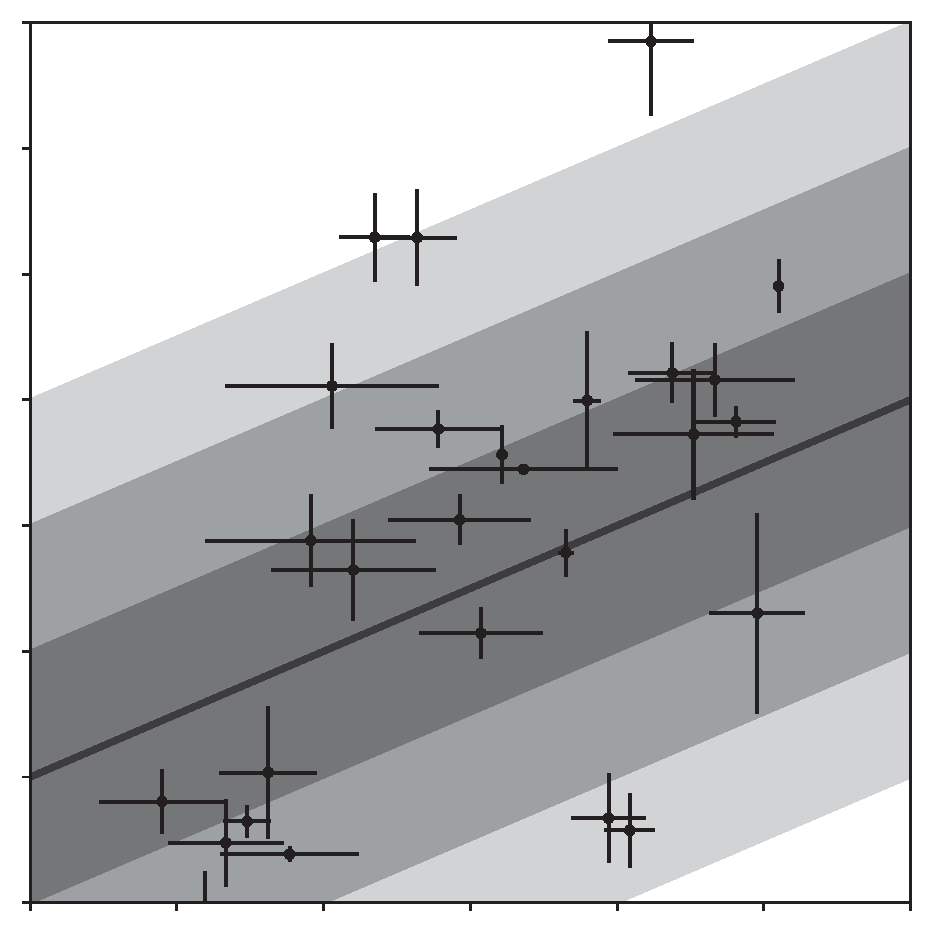
\includegraphics[width=0.8\linewidth]{figures/slopexample.eps}
    \caption{Example dataset and underlying model distribution where the scatter of the data cannot solely be accounted for by the error bars, which must be parameterized as extrinsic scatter, or \textit{slop}. Model distribution is shown with $1-$, $2-$ and $3\sigma$ confidence regions for the slop of the model, to properly account for the uncertainty in the dataset.}
    \label{fig:slopexample}
\end{figure}

In the following section, we will begin to explore how a likelihood function describing a model for this ``worst case'' type of dataset can be defined, by connecting the extrinsic and intrinsic probability distributions of the dataset with the model itself.

\subsection{The Likelihood Function}
The derivation below closely follows \textcite{trotter}, where the TRK statistic was initially formulated. In order to consider fitting a model to data, we must first determine how to quantify the goodness of fit for such a model, given some distribution of $N$ measurements described in the previous section. I define part of the model as some probability distribution $g(x,y)$ that is convolved along some model curve function $y_c(x;\vartheta_m)$, where $\vartheta_m$ is the set of parameters that define the functional form of the model. Then, in order to properly represent the scatter of the data, I define the full model distribution by convolving this with a 2D Gaussian distribution that characterizes the slop, with widths defined by the parameters $\sigma_x$ and $\sigma_y$. This representation of the model can be difficult to conceptualize, but it is necessary in order to work with the most general, Bayesian treatment of a two-dimensional uncertain dataset. A visualization of this is shown in Figures \ref{fig:model} and \ref{fig:model_zoomedin}.

\begin{figure}
    \centering
    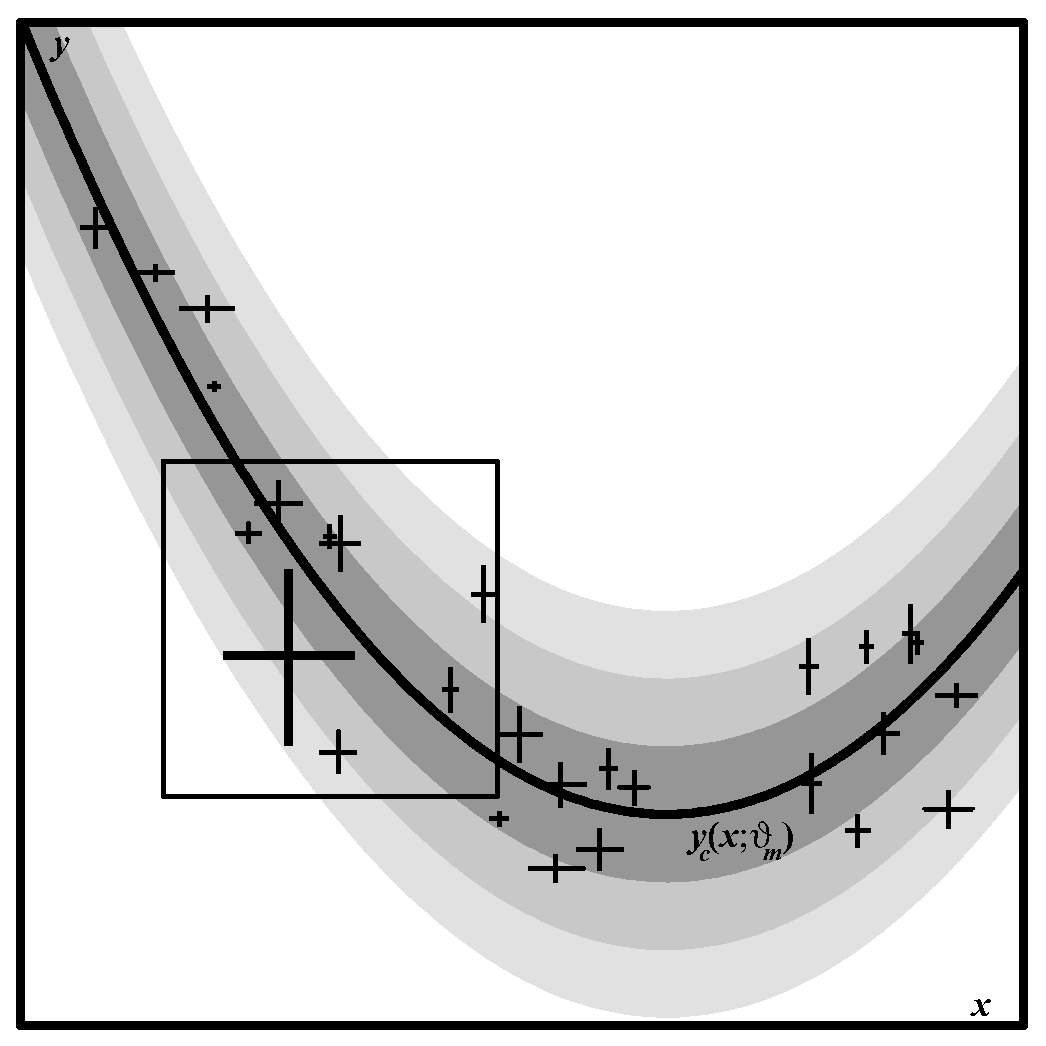
\includegraphics[width=0.8\linewidth]{figures/model.eps}
    \caption{Visualization of some two-dimensional dataset (from \textcite{trotter}) with both intrinsic and extrinsic scatter in two dimensions, and accompanying model distribution with $1-$, $2-$ and $3\sigma$ confidence regions for the extrinsic scatter/slop of the model represented by the shaded regions. Inset box is shown zoomed in Fig. \ref{fig:model_zoomedin}.}
    \label{fig:model}
\end{figure}

\begin{figure}
    \centering
    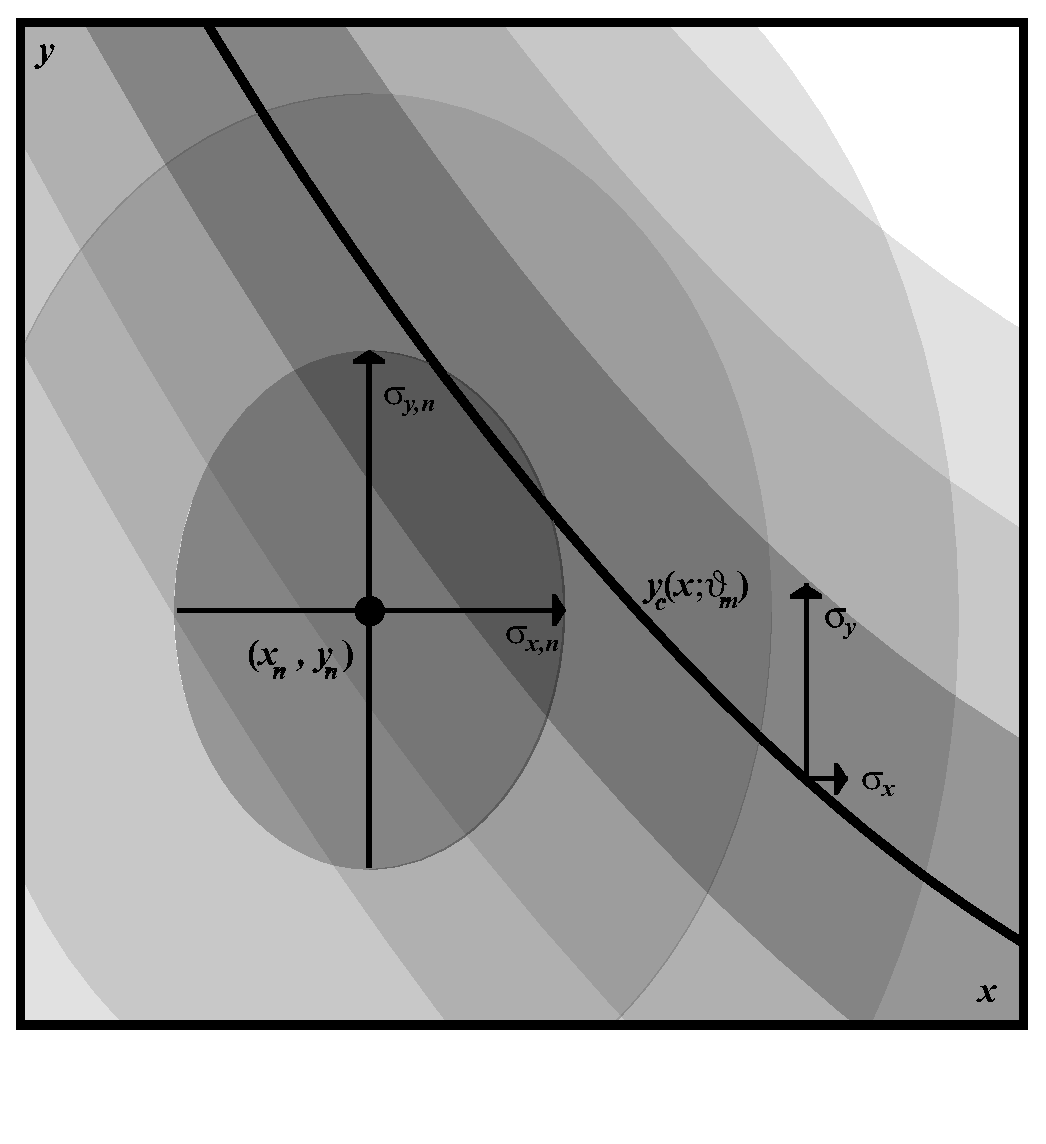
\includegraphics[width=0.8\linewidth]{figures/model_zoomedin.eps}
    \caption{Fig. \ref{fig:model}, zoomed in, from \textcite{trotter}. Centered is a single data-point $(x_n, y_n)$ with intrinsic probability distribution defined by its' error bars/intrinsic scatter $\sigma_{x,n}, \sigma_{y,n}$, alongside a model distribution with curve $y_c(x;\vartheta_m)$ and extrinsic scatter/slop parameters $(\sigma_x,\sigma_y)$. The shaded regions represent the $1-$, $2-$ and $3\sigma$ confidence regions of the datapoint's intrinsic probability distribution, and of the extrinsic scatter-convolved model distribution.}
    \label{fig:model_zoomedin}
\end{figure}

Another way to express the (effectively 1D) model curve $y_c(x;\vartheta_m)$ is do describe it as a one-dimensional delta function along some arbitrary chosen (orthogonal) coordinate system $(u_n, v_n)$. Indicated by the subscripts of $n$, such coordinates can, in the most general case, \textit{vary between datapoints}. As such, we can express the probability density along the model curve as $g(x,y)\delta(v_n, v_{c,n}(u_n;\vartheta_m))$, where $v_{c,n}(u_n;\vartheta_m)$ is $y_c(x;\vartheta_m)$ in the $(u_n, v_n)$ coordinate system, and $\delta$ denotes the one-dimensional Dirac delta function. Also note that given that the coordinates $(u_n, v_n)$ are assumed to be orthogonal, we can always express them as a rotation from $(x,y)$.

Now that we have an expression for the probability density along the model curve, we can convolve this with the extrinsic scatter/slop distribution (again, assumed to be 2D Gaussian) to obtain the \textit{model distribution function} for a single datapoint,
\begin{equation}\label{eq:pnmod}
    p_n^\text{mod}(x',y'|\vartheta_m,\sigma_x,\sigma_y)=\displaystyle\int_{u_n}\int_{v_n}g(x,y)\delta(v_n, v_{c,n}(u_n;\vartheta_m))\mathcal{N}(x'|x,\sigma_x)\mathcal{N}(y'|y,\sigma_y)\diff v_n\diff u_n,
\end{equation}
given the definition of the convolution of two bivariate functions, where the integrals are both over $(-\infty,\infty)$ and $\mathcal{N}$ denotes the Gaussian/normal distribution
\begin{equation}
\label{eq:symnorm}
    \mathcal{N}(x'|\mu,\sigma) = \frac{1}{\sqrt{2\pi\sigma^2}}\exp\left(-\frac{1}{2}{\frac{(x'-\mu)^2}{\sigma^2}}\right).
\end{equation}
with mean $\mu$ and standard deviation $\sigma$.

Next, we need to obtain an expression for the full \textit{joint} probability of a single datapoint with the model distribution function $p_n^\text{mod}$ for that datapoint. The \textit{intrinsic} probability for a single datapoint comes from the error bars for that datapoint, and is found with
\begin{equation}\label{eq:pnint}
    p_n^\text{int}(x',y'|x_n,y_n,\sigma_{x,n}, \sigma_{y,n}) = \mathcal{N}(x'|x_n,\sigma_{x,n})\mathcal{N}(y'|y_n,\sigma_{y,n}).
\end{equation}
again assuming Gaussian error bars. From here, we can find the joint probability of some $n^\text{th}$ datapoint with the model distribution by integrating the product of the two distributions $p_n^\text{mod}$ and $p_n^\text{int}$ over $x'$ and $y'$, as
\begin{align}\label{eq:pn}
p_n(\vartheta_m,\sigma_x,\sigma_y|x_n,y_n,\sigma_{x,n},\sigma_{y,n}) &= \nonumber
\int_{x^\prime}\int_{y^\prime}\int_{u_n}\int_{v_n}{g(x,y)\delta(v_n-v_{c,n}(u_n;\vartheta_m))} \times \nonumber \\
\mathcal{N}(x'|x,\sigma_x)\mathcal{N}(y'|y,\sigma_y)&\mathcal{N}(x'|x_n,\sigma_{x,n})\mathcal{N}(y'|y_n,\sigma_{y,n})\diff v_n \diff u_n \diff y^\prime \diff x^\prime \, .
\end{align}

Next, the likelihood function is defined to be the product of all $N$ of the joint probabilities of the datapoints, as
\begin{equation}\label{eq:likelibasic}
    \mathcal{L}=\prod\limits_{n=1}^Np_n(\vartheta_m,\sigma_x,\sigma_y|x_n,y_n,\sigma_{x,n},\sigma_{y,n}),
\end{equation}
so in theory, our work of finding an expression for the likelihood is done. However, given the four integrals in Equation \eqref{eq:pn}, this solution is quite computationally intractable. In order to obtain a practical likelihood, a few simplifying, but reasonable approximations need to be made, following \textcite{trotter}.

\subsection{An Analytical Approximation of the Likelihood}
\label{sec:tgtpts}
To begin, we can simplify the expression for the joint probability $p_n$ by noting that the $(x',y')$ integral in Equation \eqref{eq:pn} can be evaluated analytically, which gives
\begin{align}\label{eq:pnsimp}
& p_n(\vartheta_m,\sigma_x,\sigma_y|x_n,y_n,\sigma_{x,n},\sigma_{y,n}) = \nonumber\\
& \int_{u_n}\int_{v_n}{g(x,y)\delta(v_n-v_{c,n}(u_n;\vartheta_m))}\mathcal{N}(x|x_n,\Sigma_{x,n})\mathcal{N}(y|y_n,\Sigma_{y,n})\diff v_n \diff u_n \,,
\end{align}
where $(\Sigma_{x,n}, \Sigma_{y,n})$ are the quadrature sums of both the intrinsic and extrinsic scatters:
\begin{align}\label{eq:bigsigs}
\Sigma_{x,n} & \equiv \left( \sigma_{x,n}^2 + \sigma_x^2 \right)^{1/2} \nonumber\\
\Sigma_{y,n} & \equiv \left( \sigma_{y,n}^2 + \sigma_y^2 \right)^{1/2} \, . 
\end{align}
What is the significance of these terms? In the words of \textcite{trotter}, Equation \eqref{eq:pnsimp} indicates that the joint probability of some $n^\text{th}$ datapoint with the model distribution is proportional to the integral of the effectively one-dimensional probability density along the model curve through a two dimensional \textit{convolved} Gaussian, whose widths are the quadrature sums of the intrinsic and extrinsic uncertainties in each direction, $\Sigma_{x,n}$ and $\Sigma_{y,n}$. In other words, Fig. \ref{fig:model_zoomedin} is equivalent to \ref{fig:datapoint}.

\begin{figure}
    \centering
    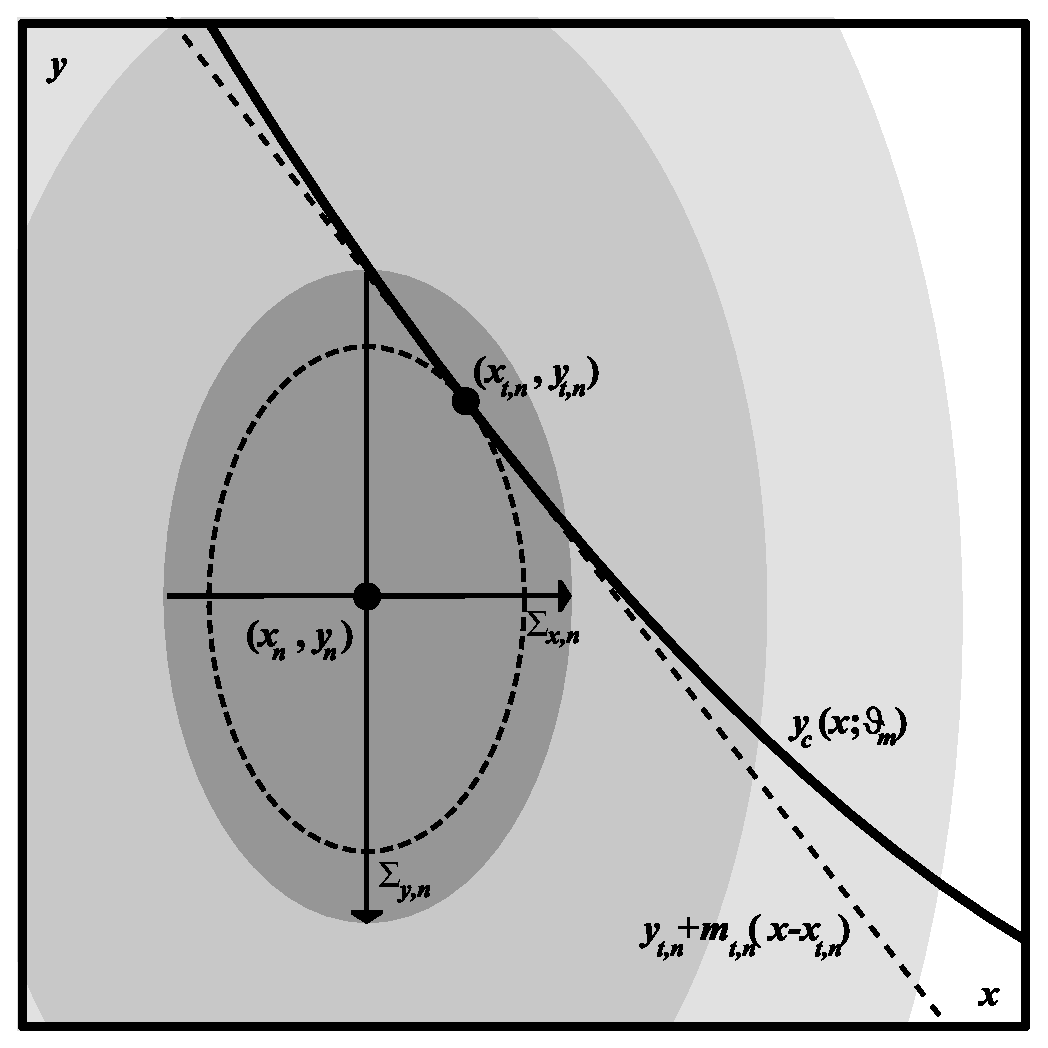
\includegraphics[width=0.8\linewidth]{figures/datapoint.eps}
    \caption{Visualization of some datapoint $(x_n,y_n)$ with convolved error ellipse defined by the extrinsic-intrinsic convolved error bars $(\Sigma_{x,n},\Sigma_{y,n})$, alongside some model curve $y_c(x)$. Also shown is the approximation of the non-linear model as a line tangent to the error ellipse at point $(x_{t,n},y_{t,n})$.}
    \label{fig:datapoint}
\end{figure}

To further simplify Equation \eqref{eq:pnsimp} (i.e., remove the integrals), I'll begin by making the first approximation: that the intrinsic probability density along the model curve $g(x,y)$ varies slowly with respect to the scale of the size of the convolved error ellipse described by $\Sigma_{x,n}$ and $\Sigma_{y,n}$. This will make $g(x,y)$ approximately constant, such that it can be pulled out of the integral in Equation \eqref{eq:pnsimp}. Next, I will assume that the model curve $y_c(x;\vartheta_m)$ is approximately linear over this same scale; specifically, I will approximate $y_c$ as a line $y_{t,n}(x)$ passing through the point $(x_{t,n},y_{t,n})$ where $y_c$ is tangent to the convolved error ellipse, with some slope $m_{t,n}$ (see Fig. \ref{fig:datapoint}), i.e.
\begin{equation}\label{eq:yclin}
    y_c(x)\approx y_{t,n} + m_{t,n}(x-x_{t,n}).
\end{equation}

If, at some position $x$, the model curve $y_c(x;\vartheta_m)$ is tangent to the error ellipse at some $(x_{t,n},y_{t,n})$, then we have the relation 
\begin{equation}\label{eq:tpoint1}
\frac{(y_c(x;\vartheta_m)-y_n)^2}{\Sigma_{y,n}^2}+\frac{(x-x_n)^2}{\Sigma_{x,n}^2} =  \frac{(y_{t,n}-y_n)^2}{\Sigma_{y,n}^2}+\frac{(x_{t,n}-x_n)^2}{\Sigma_{x,n}^2}\, ,
\end{equation}
which is the condition for $(x, y_c(x;\vartheta_m))$ to be a tangent point. Differentiating this equation with respect to $x$ gives
\begin{equation}\label{eq:tpoint2}
\dv{}{x}\left({\frac{(y_c(x;\vartheta_m)-y_n)^2}{\Sigma_{y,n}^2}+\frac{(x-x_n)^2}{\Sigma_{x,n}^2}}\right)=0 \, ,
\end{equation}
which implies that the tangent point is equivalent to the point on $y_c$ that \textit{minimizes the radial distance} to the centroid of the error ellipse. Evaluating the derivative gives us an equation that can be \textit{implicitly} solved for $x=x_{t,n}$,
\begin{equation}\label{eq:tpoint}
(y_c(x)-y_n)\dv{y_c(x;\vartheta_m)}{x}\Sigma_{x,n}^2+(x-x_n)\Sigma_{y,n}^2 = 0 \, ,
\end{equation}
given some model curve and datapoint.%\footnote{The actual method used to solve for these tangent points is covered in \S\ref{cha:code}.}.% For non-monotonic curves, there may be multiple such tangent points for a given datapoint; in this case, we take the tangent point that maximizes the joint probability.

Finally, given these two assumptions, the joint probability of the $n^\text{th}$ datapoint and the model distribution of Equation \eqref{eq:pnsimp} can be simplified by integrating over $v_n$, as
\begin{align}\label{eq:pnappint}
p_n(\vartheta_m,\sigma_x,\sigma_y|x_n,y_n,\sigma_{x,n},\sigma_{y,n}) \approx g(x_n,y_n)\int_{-\infty}^{\infty}{\mathcal{N}(x|x_n,\Sigma_{x,n})\mathcal{N}(y_c(x;\vartheta_m)|y_n,\Sigma_{y,n})\diff u_n}\, ,
\end{align}
given the ``selecting'' property of the delta function on the Gaussian along $y$. By using the chain rule substitution $\diff u_n = \dv{u_n}{x}\diff x$, $y_c(x;\vartheta_m)\approx y_{t,n}+m_{t,n}(x-x_{t,n})$ from Equation \eqref{eq:yclin}, and integrating over $x$, we have finally arrived at an analytic expression for $p_n$:\footnote{Here, we have also implicitly made an additional approximation: that the efficiency of which the measured data samples the \textit{true} model distribution is approximately constant along the scale(s) of $(\sigma_{x,n}, \sigma_{y,n})$ and $(\sigma_x,\sigma_y)$. This is unnecessary to delve into for the purposes of this work, but for an explicit inclusion of this, see \S2.2.1 of \textcite{trotter}.} 
\begin{align}\label{eq:pnanaly}
&p_n(\vartheta_m,\sigma_x,\sigma_y|x_n,y_n,\sigma_{x,n},\sigma_{y,n}) \\ &\approx g(x_n,y_n)\dv{u_n}{x}\mathcal{N}\left(y_n\left|\right.y_{t,n}+m_{t,n}(x_n-x_{t,n}),\sqrt{m_{t,n}^2\Sigma_{x,n}^2+\Sigma_{y,n}^2}\,\right) \nonumber \, .
\end{align}

The likelihood function is the joint probability of the model distribution with all of the datapoints, and the \textit{best fit} model parameters are defined as the parameters that, when plugged into the likelihood, maximize it. In other words, the likelihood is the product of all $N$ of the individual datapoints' joint probability distributions. In practice, rather than choosing to \textit{maximize} $\mathcal{L}$ to determine the best fit, it is much more common to \textit{minimize} $-2\ln\mathcal{L}$ (or some proportion thereof) in order to determine the best fit model parameters, for reasons of computational flexibility. In the simplifying ``traditional'' case of no error bars in $x$ and no slop whatsoever, $-2\ln\mathcal{L}$ is equivalent to the $\chi^2$ ``goodness-of-fit'' statistic, $\chi^2=\sum\limits_{n=1}^N\left[(y - y_c(x;\vartheta_m))/\sigma_{y,n}\right]^2$. As such, in our general case, $-2\ln\mathcal{L}$ is analogous to $\chi^2$, and has the form of
\begin{align}\label{eq:likegen}
-2\ln\mathcal{L} &= -2\sum_{n=1}^{N}{\ln p_n(\vartheta_m,\sigma_x,\sigma_y|x_n,y_n,\sigma_{x,n},\sigma_{y,n})} \nonumber \\
&=\sum_{n=1}^{N}\frac{\left[y_n-y_{t,n}-m_{t,n}(x_n-x_{t,n})\right]^2}{m_{t,n}^2\Sigma_{x,n}^2+\Sigma_{y,n}^2} -2\sum_{n=1}^{N}\ln\left(\dv{u_n}{x}\frac{1}{\sqrt{m_{t,n}^2\Sigma_{x,n}^2+\Sigma_{y,n}^2}}\right) + C \, ,
\end{align}
following Equations \eqref{eq:likelibasic} and \eqref{eq:pnanaly}, where $C$ is a constant\footnote{The explicit form of the constant $C$ is given in \textcite{trotter}, which isn't necessary for the purposes of this paper, as constant offsets are arbitrary for the process of likelihood maximization.}.

Recall that the rotated coordinate system $(u_n, v_n)$ in which the 1D model curve $\delta(v_n, v_{c,n}(u_n;\vartheta_m))$ is defined can be chosen at will, including the usage of different coordinates for different datapoints. As will be described in \S\ref{sec:compare}, different choices of these coordinates/of $\dv{u_n}{x}$ will give different statistics, with noticeably different properties. The following section will show how a certain choice of these coordinates will lead to the TRK statistic.

\subsection{The TRK Likelihood}
\label{sec:likelihood}
As shown in Equation \eqref{eq:likegen}, The arbitrary choice of the rotated coordinates $(u_n,v_n)$ and therefore the factor $\dv{u_n}{x}$ will be what defines a given statistic. While various choices for $\dv{u_n}{x}$ that lead to different statistics with different properties will be explored in \S\ref{sec:compare}, for now I will only examine the choice that leads to the TRK statistic, which is advantageous over other such statistics for reasons that will be addressed in \S\ref{sec:compare}.

The TRK statistic is defined such that for some $n^\text{th}$ datapoint, $u_n$ is chosen to be perpendicular to the line segment connecting the centroid of the datapoint $(x_n,y_n)$ with the tangent point $(x_{t,n},y_{t,n})$ discussed in the previous section. This choice results in a likelihood of the form
\begin{align}\label{eq:TRK}
\mathcal{L}^{\mathrm {TRK}} & \propto \prod_{n=1}^{N}{ \sqrt{\frac{m_{t,n}^2\Sigma_{x,n}^2+\Sigma_{y,n}^2}{m_{t,n}^2\Sigma_{x,n}^4+\Sigma_{y,n}^4}}\exp\left\{{-\frac{1}{2}\frac{\left[y_n-y_{t,n}-m_{t,n}(x_n-x_{t,n})\right]^2}{m_{t,n}^2\Sigma_{x,n}^2+\Sigma_{y,n}^2}}\right\}} \nonumber \\ -2\ln\mathcal{L}^{\mathrm{TRK}} &= \sum_{n=1}^{N}{\frac{\left[y_n-y_{t,n}-m_{t,n}(x_n-x_{t,n})\right]^2}{m_{t,n}^2\Sigma_{x,n}^2+\Sigma_{y,n}^2}} - \sum_{n=1}^{N}{\ln\left(\frac{m_{t,n}^2\Sigma_{x,n}^2+\Sigma_{y,n}^2}{m_{t,n}^2\Sigma_{x,n}^4+\Sigma_{y,n}^4}\right)} + C \, ,
\end{align}
which is the central equation of this work. One important property of the TRK statistic is that \textit{it is essentially a one-dimensional $\chi^2$-like statistic that is measured in the direction of the tangent point}\footnote{The derivation of this is beyond the scope of this work, but is found in \textcite{trotter}.}. For a visualization of the geometry of the TRK statistic, see Figure \ref{fig:datapointcolor}. Hereafter, I will sometimes use the shorthand  $\chi^2_\text{TRK}\equiv-2\ln\mathcal{L}^\text{TRK}$, especially in Chapter \ref{cha:code1} where it is frequently used.
% \begin{align}\label{eq:TRK}
% \mathcal{L}^{\mathrm {TRK}} & \propto \prod_{n=1}^{N}{ w_n\sqrt{\frac{m_{t,n}^2\Sigma_{x,n}^2+\Sigma_{y,n}^2}{m_{t,n}^2\Sigma_{x,n}^4+\Sigma_{y,n}^4}}\exp\left\{{-\frac{1}{2}w_n\frac{\left[y_n-y_{t,n}-m_{t,n}(x_n-x_{t,n})\right]^2}{m_{t,n}^2\Sigma_{x,n}^2+\Sigma_{y,n}^2}}\right\}}
% \end{align}

\begin{figure}
    \centering
    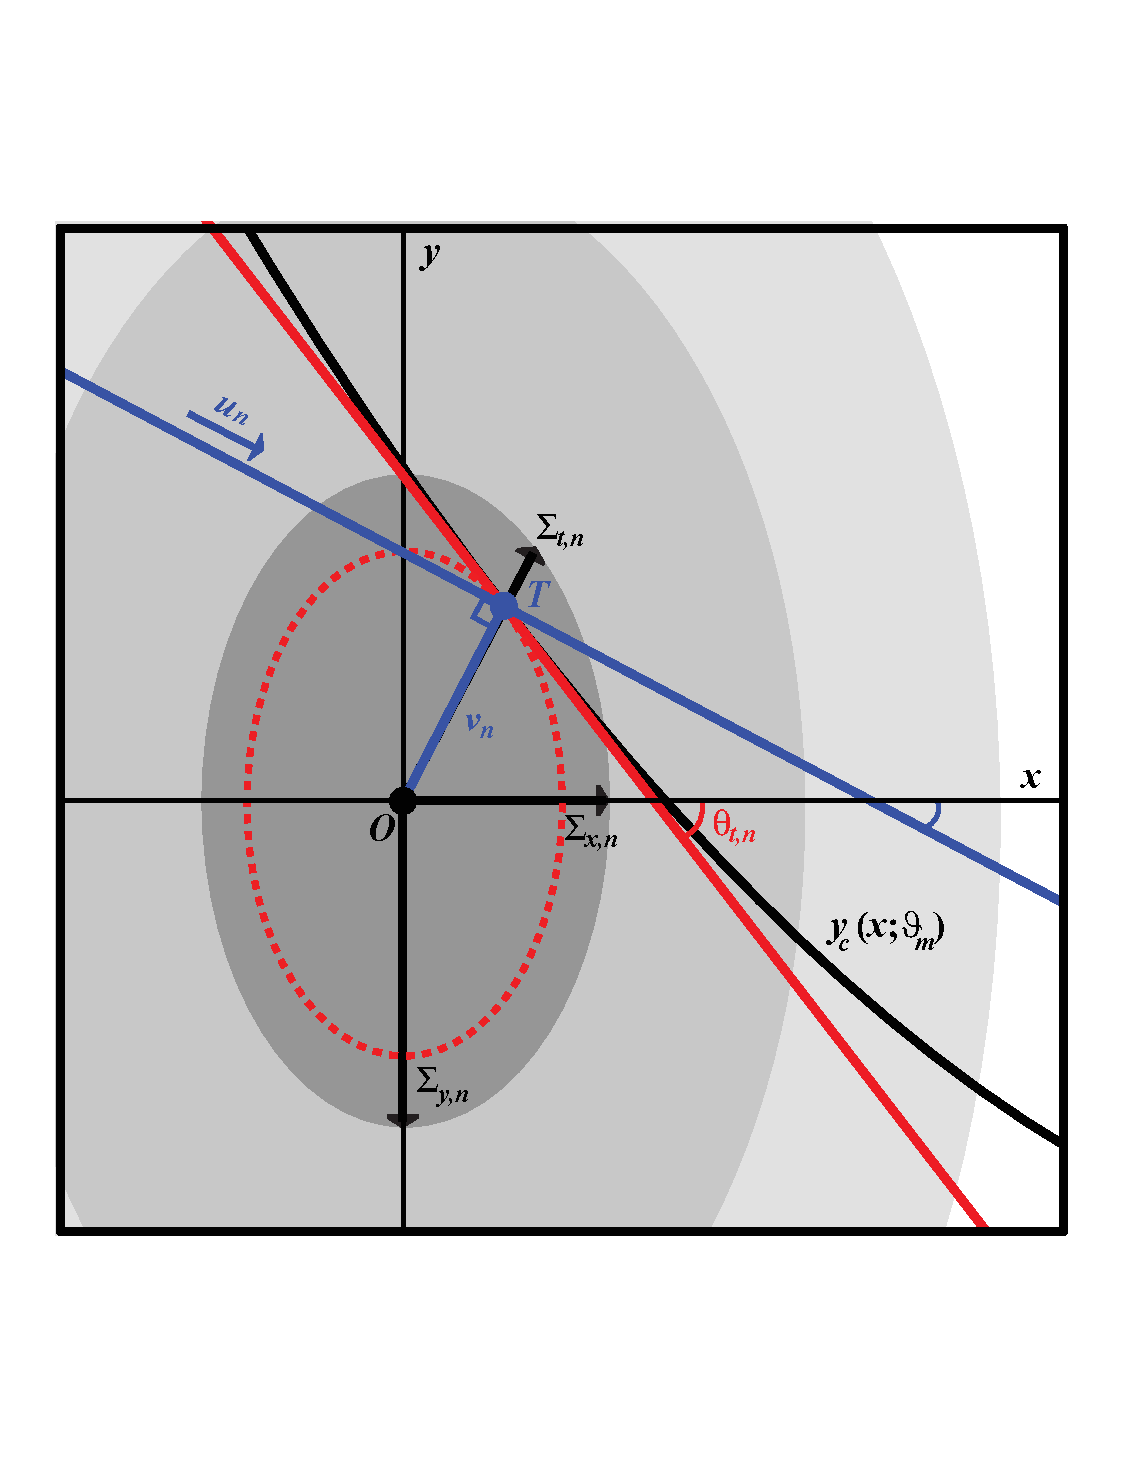
\includegraphics[width=0.8\linewidth]{figures/datapoint_med_simp.eps}
    \caption{Illustration of the geometry of the TRK statistic modified from \textcite{trotter}, given some datapoint and model. The datapoint is centered at $(x_n,y_n)$ (point $O$), with convolved error ellipse described by the widths $(\Sigma_{x,n},\Sigma_{y,n})$ (Equation \eqref{eq:bigsigs}). The model curve $y_c(x;\vartheta_m)$ is tangent to the convolved error ellipse at tangent point $(x_{t,n},y_{t,n})$ (point $T$), and the red line is the linear approximation of the model curve, with slope $m_{t,n}=\tan\theta_{t,n}$. The blue line indicates the rotated coordinate axis $u_n$ for the TRK statistic, perpendicular to the $v_n$ axis.}
    \label{fig:datapointcolor}
\end{figure}             %% this is a suggestion: you have to create this file on demand
\chapter{Properties of the TRK Statistic}
\label{cha:properties}

\subsection{Invertibility}
\label{sec:invertibility}
A useful property for any two-dimensional statistic is that it is \textit{invertible}, i.e. that if fitting a dataset's $y$ vs $x$ data gives some model curve $y_c(x)$, fitting $x$ vs. $y$ gives the inverse $x_c(y)=y_c(x)^{-1}$. In the Bayesian formalism, a statistic is invertible if running these two inverted fits yields the same likelihood function (\textcite{trotter}). While mainly known to be used as a measure of the linear correlation of a dataset, one metric of invertibility is actually the ubiquitously-used Pearson Correlation Coefficient, $R^2$, of \textcite{pearson1896vii}. To see this, consider some linear model with slope $m_{yx}$ that was obtained by fitting to some $y$ vs. $x$ data. Similarly, fitting $x$ vs. $y$ for the same dataset gives some model line with slope $m_{xy}$. As shown in \textcite{trotter}, the correlation coefficient can then be found as $R^2\equiv m_{xy}m_{yx}$; therefore, if the statistic used to fit is invertible, and therefore $m_{xy}=1/m_{yx}$, we have that $R^2=1$. Proved by \textcite{trotter}, \textcite{the TRK statistic is completely invertible}. Therefore, by definition $R^2=1$ always for the TRK statistic, meaning that fitting results can always be trusted under inversion.

\subsection{Scalability}
\label{sec:scalability}
Another important property of any statistic, although not immediately obvious, is its \textit{scalability}. Here, a statistic is defined to be \textit{scalable} if re-scaling the data along the $x-$ or $y-$ axis does not change the best fit arrived at from maximizing the likelihood. If a statistic is not scalable, then the best fit will \textit{depend} on the choice of units of measurement (or bases of the data axis if converted to some non-linear basis e.g. logarithmic), which can easily create unwanted behavior when fitting (see e.g. \textcite{trotter}), given that there is usually never any \textit{a priori} to choose some set of units over another.

To examine the scalability of the TRK statistic, we will begin by noting that the statistic is invariant if both $x-$ and $y-$ axes are rescaled by the same factor, shown in \textcite{trotter}. As such, any rescaling that potentially affects the TRK statistic can always be defined as rescaling only the $y-$axis by some numerical factor $s$\footnote{Equivalently we can define $s\equiv s_y/s_x$, where $s_y$ is the standalone rescaling of the $y-$axis, and $s_x$ is the same for the $x-$axis.}. In order to see the effect of data rescaling within the TRK statistic, I multiply all $y-$axis dependent terms by some $s$ within the TRK likelihood of Equation \eqref{eq:TRK}, which gives
\begin{align}\label{eq:TRK_scaled}
\mathcal{L}_s^{\mathrm {TRK}} & \propto \prod_{n=1}^N{ \sqrt{\frac{m_{t,n}^2\Sigma_{x,n}^2+\Sigma_{y,n}^2}{m_{t,n}^2\Sigma_{x,n}^4+s^2\Sigma_{y,n}^4}}\exp\left\{-\frac{1}{2}\frac{\left[y_n-y_{t,n}-m_{t,n}(x_n-x_{t,n})\right]^2}{m_{t,n}^2\Sigma_{x,n}^2+\Sigma_{y,n}^2}\right\}} \nonumber \\*
& \not\propto \mathcal{L}^{\mathrm {TRK}} \mbox{~~for a fixed $s$}\, .
\end{align}
As such, the standalone TRK statisic is \textit{not} scalable, so different choices of scale will result in different best fit model parameters, including slop/extrinsic scatter ($\sigma_x,\sigma_y$). Not only this, but it is impossible to determine anything about the relative fitness of best fits solely given numerical values of the likelihood function; what this means in practice is that the scaling factor $s$ can not be fit to as a model parameter (\textcite{trotter}). However, we will show in the following section that there \textit{is} a way to quantitatively compare TRK fits done at different scales, so that this hurdle can be negated.

\subsection{The TRK Correlation Coefficient}
\label{sec:TRKcorr}
To begin, consider two TRK best fits gained from maximizing the likelihood (Equation \eqref{eq:TRK_scaled}) at different scales (i.e. different values for $s$), given some model and dataset. Because the TRK statistic is completely invertible, the Pearson Correlation Coefficient $R^2$ is $1$ for both fits. As such, in order to compare the two fits,  a new correlation coefficient needs to be defined that can quantify the variance of the statistic's predictions between them. By convention, the new coefficient should follow similar properties to $R^2$, insofar that it is restricted to the range of $[0,1]$, and that it equals 1 if the two best fit lines begin compared have the same slope (plotted in the same scale space).

I will begin with the case of linear fits, and continue on to generalize to arbitrary non-linear models. \textcite{trotter} introduced a new correlation coefficient $R^2_\text{TRK}$ that is a function of the \textit{difference} of the slopes of the models, rather than the \textit{ratio}, as opposed to the Pearson $R^2$ (see \S\ref{sec:invertibility}). The \textit{scale-dependent} TRK correlation coefficient is defined as
\begin{equation}\label{eq:r2TRKab}
R_{\mathrm{TRK}}^{2}(a,b)\equiv \tan^2\left(\frac{\pi}{4}-\frac{\left|\theta_a-\theta_b\right|}{2}\right) \, .
\end{equation}
given a linear fit at $s=a$ with slope $m_a=\tan{\theta_a}$, and another at $s=b$ with slope $m_b=\tan{\theta_b}$\footnote{$R^2_\text{TRK}$ compares the \textit{angles} (off of the $x$-axis) $\left(\theta_a,\theta_b\right)$ of the lines rather than the \textit{slopes} $\left(m_a,m_b\right)$ for numerical efficacy, given that the former are restricted to the range of $\left(-\frac{\pi}{2},\frac{\pi}{2}\right)$, while the latter can be anywhere within $(-\infty,\infty)$.}. Clearly, if the two lines have the same slopes, $R^2_\text{TRK}=1$ as desired, and if the two lines differ in slope angle by $90^\circ$, i.e. they are orthogonal, $R^2_\text{TRK}=0$. Now that the difference between TRK fits at different scales can be compared, how do we determine the best scale at which to run a fit?

Consider how rescaling will affect the slop parameters $\sigma_x$ and $\sigma_y$, i.e. how the total slop is distributed between these two parameters. \textcite{trotter} showed that in the limit of slop-dominated data (i.e. arbitrarily small/zero error bars $\left\{\sigma_{x,n},\sigma_{y,n}\right\}$ as compared to the extrinsic scatter/slop), $s\rightarrow 0$, $\sigma_x\rightarrow 0$; similarly, as $s\rightarrow \infty$, $\sigma_y\rightarrow 0$. This behavior occurs because as the scale $s$ of the dataset is changed, the distribution of the total slop between $\sigma_x$ and $\sigma_y$ is correspondingly affected. This range of $s\in[0,\infty)$ is considered to be the \textit{physically meaningful} range of fits. In the case of a dataset with non-zero error bars, this physically meaningful range becomes some subset interval $[a,b]\subset[0,\infty)$, where the number $a$ is described as the \textit{minimum scale}, while $b$ is the \textit{maximum scale}, as $\lim\limits_{s\rightarrow a^+}\sigma_x = 0$ and $\lim\limits_{s\rightarrow b^-}\sigma_y = 0$ (from \cite{trotter})\footnote{Here, I've taken the signs of the limits to indicate the direction of one-sided approach.}. As any fits done outside of this interval are inherently unphysical, there must be some optimum $s_0\in[a,b]$ that is the best scale at which to run a fit\footnote{By ``unphysical'', I mean that such scales require imaginary best fit slops, i.e. $(\sigma_x^2,\sigma_y^2)<0$ (\cite{trotter}).}.

\label{par:scaleopscheme}In order to determine the optimum scale $s_0$, the following iterative approach defined within \textcite{trotter} is used. To begin, the first approximation of $s_0$, $s_0^{(1)}$, is found to be the scale at which
\begin{equation}\label{eq:r2TRK}
R^{2}_{\mathrm{TRK}}(a,s_0^{(1)}) = R^{2}_{\mathrm{TRK}}(s_0^{(1)},b) \equiv R^2_{\mathrm{TRK}} \, .
\end{equation}
From here, we shift from the $s=1$ space to this $s=s_0^{(1)}$ space, where the angles of the lines follow the transformation $\theta\rightarrow \arctan\left(s_0^{(1)}\tan\theta\right)$. The analysis of Equation \eqref{eq:r2TRK} is then repeated in this new space to determine the next approximation for the optimum scale, $s_0^{(2)}$, i.e. finding the $s_0^{(2)}$ such that,
e.g. in the case of a linear model,
\begin{align}\label{eq:r2TRKnewscalelin}
R^2_{\mathrm{TRK}} & \equiv \tan^2\left(\frac{\pi}{4}-\frac{\left|\arctan (s_0^{(1)}\tan\theta_a)-\arctan (s_0^{(1)}\tan\theta_{s_0^{(2)}})\right|}{2}\right) \nonumber \\
& =
\tan^2\left(\frac{\pi}{4}-\frac{\left|\arctan (s_0^{(1)}\tan\theta_{s_0^{(2)}})-\arctan (s_0^{(1)}\tan\theta_b)\right|}{2}\right) \, ,
\end{align}
where $\theta_{s_0^{(2)}}$ is the position angle of the best-fit line at scale $s_0^{(2)}$, as measured in $s=1$ space. From here, we set $s_0^{(2)}\rightarrow s_0^{(1)}$, and repeat until convergence to the final value of $s_0$. It is at this optimum scale that we actually run fits, compute model parameter uncertainties (see \S\ref{sec:MCMC}), etc. The details of how Equation \eqref{eq:r2TRK} is solved in practice to determine $s_0$ are given in \S\ref{sec:scaleop}.

The TRK correlation coefficient as given in Equation \eqref{eq:r2TRKab} can only be used for linear models. As such, \textcite{trotter} presented a logical generalization to nonlinear models, as the average of the differences of the slope angles at all $N$ tangent points at two scales $a$ and $b$:
\begin{equation}\label{eq:R2TRKgen}
R_{\mathrm{TRK}}^{2}(a,b)\equiv \frac{1}{N}\sum_{n=1}^{N}{\tan^2\left(\frac{\pi}{4}-\frac{\left|\theta_{t,n;a}-\theta_{t,n;b}\right|}{2}\right)} \, .
\end{equation}
Here, $\theta_{t,n;a}=\arctan m_{t,n;a}$ and $\theta_{t,n;b}=\arctan m_{t,n;b}$ are the position angles of the best-fit curves at the tangent point to the $n^\text{th}$ datapoint at scales $a$ and $b$, respectively. This expression for $R_{\mathrm{TRK}}^{2}$ can then be used to determine $s_0$ using the same method described by the previous section and Equation \eqref{eq:r2TRK}; in this case then, Equation \eqref{eq:r2TRKnewscalelin} becomes
\begin{align}\label{eq:r2TRKnewscalenonlin}
R^2_{\mathrm{TRK}} & \equiv \frac{1}{N}\sum_{n=1}^{N}\tan^2\left(\frac{\pi}{4}-\frac{\left|\arctan (s_0^{(1)}\tan\theta_{t,n;a})-\arctan (s_0^{(1)}\tan\theta_{s_0^{(2)}})\right|}{2}\right) \nonumber \\
& =
\frac{1}{N}\sum_{n=1}^{N}\tan^2\left(\frac{\pi}{4}-\frac{\left|\arctan (s_0^{(1)}\tan\theta_{s_0^{(2)}})-\arctan (s_0^{(1)}\tan\theta_{t,n;b})\right|}{2}\right) \, .
\end{align}

With this, we have covered all of the foundations and properties of the TRK statistic that are needed to describe how TRK fits are completed in practice. In the next chapter, I will delve into the suite of algorithms that I created to perform fitting, scale optimization, model parameter distribution generation, and other core fitting algorithms.
%In the procedure described above, we defined both R02
%TRF(a, b) (Equation 2.44), which
%is a measure of the difference between the TRF fits at the two physically meaning-
%ful extremes of scale, and R2T
%RF (Equation 2.45), which is a measure of the difference
%between the fit at the optimum scale s0 and the fit at either extreme.
%\addcontentsline{toc}{chapter}{The TRK Fitting Algorithm}
\chapter{The TRK Codebase: Core Algorithms}
\label{cha:code1}
% From Adam's thesis:
%For non-linear model curves, the tangent point must be found numerically. Depending on the functional form of yc(x; m), this point can be bracketed and found by any num-ber of numerical root-finding algorithms.4 We note that in the case of non-monotonic curves, there may be two or more such tangent points for each datapoint; in those cases, we choose the one that maximizes the joint probability.
% USE ALGORITHM ENVIRONMENTS
The previous chapter introduced all of the formalism needed to use the TRK statistic in principle, but how can TRK fits be done in practice? What are the implementational details? What options and configurations are available when using the TRK statistic? While the statistic itself was created by \textcite{trotter}, it was only implemented in the form of a genetic algorithm-based scientific codebase for testing. In order to have a production-quality codebase for the usage of TRK, I created a new suite of algorithms from scratch in C++, that completely overhauls how TRK fits are computed, including many additions and optimizations as compared to the previous codebase. With this new codebase, TRK can be used in a fully customizable, yet easy-to-use manner, with a host of options. The code and full documentation can be downloaded at \url{https://skynet.unc.edu/rcr/calculator/downloads}.

The first part of this chapter will discuss the implementation of the central part of the TRK statistic, the TRK likelihood function $\mathcal{L}^\text{TRK}$ of Equation \eqref{eq:TRK}, that is maximized to obtain best fits. Here, I will explore my the algorithms that I use to determine the tangent points described by Equation \eqref{eq:tpoint}, and maximize $\mathcal{L}^\text{TRK}$ with respect to all model parameters---including slop---to obtain best fits. Following this, I will delve into the routine that is used to determine the optimum fitting scale $s_0$, using the formalism described in \S\ref{sec:TRKcorr}. From there, I will explore the Monte Carlo methods used to generate the full probability distributions and uncertainties of model parameters.

\section{Tangent Point Finding}
\label{sec:tgtfinder}
As shown in \S\ref{sec:tgtpts} and \S\ref{sec:likelihood}, for a given model curve $y_c(x;\vartheta_m)$ and datapoint $(x_n,y_n)$, the point where the convolved error ellipse of the datapoint described by the convolved error parameters $(\Sigma_{x,n}, \Sigma_{y,n})$ of Equation \eqref{eq:bigsigs} is tangent to the model curve, $(x_{t,n},y_{t,n})$, is a central part of the TRK likelihood $\mathcal{L}^\text{TRK}$ (Equation \eqref{eq:TRK}). Any time that the likelihood must be computed for a new set of model and slop parameters, all $N$ of these tangent points must be re-computed, and efficiently.

Recall that in order to determine such a tangent point $x_{t,n}$ (and therefore $y_{t,n}=y_c(x_{t,n};\vartheta_m)$), Equation \eqref{eq:tpoint} must be solved implicitly for $x_{t,n}$ in the general case of some nonlinear model. In more practical terms, this means that the root(s) along the $x-$axis of the left hand side of Equation \eqref{eq:tpoint} are such tangent point(s). To determine these tangent points, I use (a slightly modified version of) the Two-Point Newton-Raphson algorithm created by \textcite{tiruneh2013two} to find the roots of Equation \eqref{eq:tpoint}. This algorithm has a number of benefits over other root-finding methods such as bisection and the traditional Newton-Raphson method, especially when dealing with complicated nonlinear functions that otherwise give convergence and speed issues. My pseudocode implementation of it is shown in Algorithm \ref{algo:tpNR}, and my primary modification to the method of Tiruneh et. al is that during the course of the algorithm, if it's possible to use the bisection root-finding algorithm, it will switch to that.
\begin{algorithm}
\label{algo:tpNR}
\caption{Modified Two-Point Newton-Raphson algorithm for finding a single tangent point.}
\DontPrintSemicolon
    \SetKwInOut{Input}{Input}
    \SetKwInOut{Output}{Output}
    \SetKwProg{Fn}{Function}{}{}
    \Fn{TwoPointNR}{
    \Input{Model parameters $\vartheta_m$, datapoint $(x_n,y_n)$, its convolved errors $(\Sigma_{x,n}, \Sigma_{y,n})$, and initial tangent point guess of $x_{\text{guess}}$.}
    \Output{$x_{t,n}$}
    \Begin{
    Initialize guess of $x_{k-1}=x_{\text{guess}}$ and $x_k=x_{\text{guess}} + \Sigma_{x,n}/\sqrt{10})$\;
        \While{not converged}{
            \textit{Main Two-Pt NR loop:}\;
            $\displaystyle y_{k-1} = [y_c(x_{k-1};\vartheta_m) - y_n]\dv{y_c(x_{k-1};\vartheta_m)}{x}\Sigma_{x,n}^2 + (x_{k-1}-x_n)\Sigma_{y,n}^2$\;
            \vspace{0.3cm}$\displaystyle y_{k} = [y_c(x_{k};\vartheta_m) - y_n]\dv{y_c(x_{k};\vartheta_m)}{x}\Sigma_{x,n}^2 + (x_{k}-x_n)\Sigma_{y,n}^2$\;
            \vspace{0.3cm}$\displaystyle\dv{y_k}{x}=\left(\dv{y_c(x_{k};\vartheta_m)}{x}\right)^2 + [y_c(x_{k};\vartheta_m) - y_n]\dv[2]{y_c(x_{k};\vartheta_m)}{x}\Sigma_{x,n}^2+\Sigma_{y,n}^2$\;
            \vspace{0.3cm}$\displaystyle r=1 - \frac{y_k}{y_{k-1}}\left(\frac{y_k-y_{k-1}}{x_k-x_{k-1}}\bigg/\dv{y_k}{x}\right)$\;
            \vspace{0.3cm}$\displaystyle x_{k+1}=\left(1-\frac{1}{r}\right)x_{k-1}+\frac{x_k}{r}$\;
            \textit{Stops Two-Pt NR and performs bisection root finding routine if possible:}\;
            \If{$y_ky_{k-1}<0$}{
                $X = \{x_k,x_{k-1}\}$\;
                \Return{\textit{Bisection}(\textit{left bound}$=\min X$, \textit{right bound}$=\max X$)}\;
            }
            $x_{k-1}=x_k,\, x_k=x_{k+1}$\;
        }
        \Return{$x_{t,n}=x_k$}
    }
    }
\end{algorithm}

It is essential to note that for certain non-monotonic, nonlinear models, there can easily be multiple tangent points for a given datapoint; see Figure \ref{fig:multtgt} as an example. In this case, I take the tangent point that maximizes the joint posterior probability\footnote{I.e. for some $n^\text{th}$ datapoint, the joint posterior probability is the $n^\text{th}$ term in the product of Equation \eqref{eq:TRK}.} as the tangent point to be used when evaluating the likelihood. However, only using the rootfinder of Algorithm \ref{algo:tpNR} once per datapoint is insufficient, as some initial guess for the algorithm will always only return the same, single tangent point. In order to reliably determine \textit{all} possible tangent points for a given datapoint, to properly maximize the likelihood, I use a logical routine described in Algorithm \ref{algo:tpFinder}. The essence of this algorithm is that various initial guesses are supplied for the root-finder, using approximations for Equation \eqref{eq:tpoint} about known tangent points and other logic, until all possible tangent point-finding options have been exhausted. In general, I've found that non-periodic functions generally have no more than three tangent points for a given datapoint. Finally, I note that in the current C++ implementation of the TRK suite, the option to parallelize the determination of all $N$ tangent points for a given evaluation of $\mathcal{L}^\text{TRK}$ is provided\footnote{Parallelizing the tangent-point finder isn't always advisable for simple, linear models, as the two-point Newton-Raphson routine runs so fast with these models that the computational overhead for starting and stopping each tangent point's computational thread is greater than the power needed to actually find the tangent point itself. As such, this feature is most useful for nonlinear models.}.
\begin{figure}
    \centering
    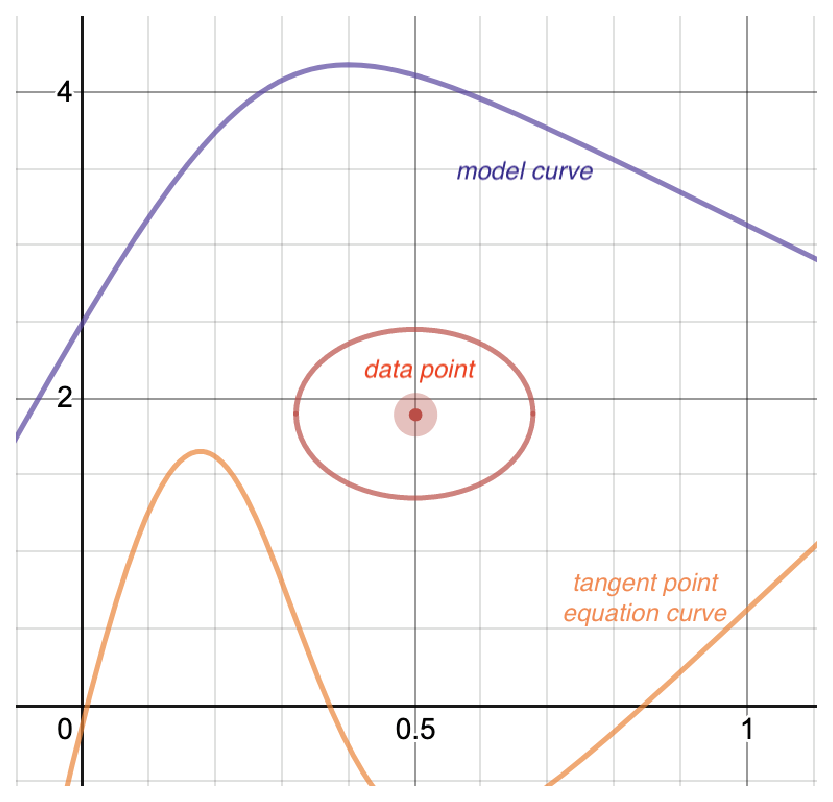
\includegraphics[width=0.6\linewidth]{figures/multtgtexample.eps}
    \caption{Example of a model curve $y_c(x;\vartheta_m)$ (purple, top) and datapoint $(x_n,y_n)$ with convolved error ellipse (red, middle) described by $(\Sigma_{x,n}, \Sigma_{y,n})$ where there are multiple points where $y_c$ is tangent to the ellipse. This translates to there being multiple solutions/roots to/of Equation \eqref{eq:tpoint}, which is plotted in orange at the bottom.}
    \label{fig:multtgt}
\end{figure}
\begin{algorithm}
\label{algo:tpFinder}
\caption{Find all possible tangent points for a given model and datapoint.}
\DontPrintSemicolon
    \SetKwInOut{Input}{Input}
    \SetKwInOut{Output}{Output}
    \SetKwProg{Fn}{Function}{}{}
    \Fn{FindAllTangentPoints}{
    \Input{Model parameters $\vartheta_m$, datapoint $(x_n,y_n)$, and its convolved errors $(\Sigma_{x,n}, \Sigma_{y,n})$.}
    \Output{Array of all tangent points $\{x_{t,n}^{i}\}$.}
    \Begin{
    Initialize empty $\{x_{t,n}^{i}\}$, and initialize $x_{\text{guess},0} = x_n$.\;
        \While{not all tangent points $x_{t,n}^{i}$ found}{
            \textit{First tangent point is the one that Two-Point Newton Raphson finds:}\;
            Append $x_{t,n}^\text{new} = $\textit{TwoPointNR}$(x_{\text{guess}} = x_{\text{guess},0})$ to $\{x_{t,n}^{i}\}$\;
            \If{New root found is same as one from previous iteration}{
                \textbf{break}\;
            }
            \If{TwoPointNR oscillating between two tangent points $x_1,x_2\in\{x_{t,n}^{i}\}$)}{
                $x_\text{mid} = $\textit{TwoPointNR}$[x_{\text{guess}} = $\textit{Midpoint}$(x_1,x_2)]$ to $\{x_{t,n}^{i}\}$\;
                {$\{x_{t,n}^{i}\} = \{x_1,x_2,x_\text{mid}\}$}\;
                \textbf{break}\;
            }
            
            \textit{Use quadratic approximation through $x_{t,n}^\text{new}$ to approximate two more tangent points if possible (see Algorithm \ref{algo:quadapprox}):}\;
            $\{x_{t,n}^\text{approx}\} = $\textit{QuadraticApprox}$(x_{t,n}^\text{new})$\;
            \If{$\{x_{t,n}^\text{approx}\}$ has 2 additional, approximate tangent points $x_\text{guess,1}, x_\text{guess,2}$}{
                Let $(x_\text{guess,1}, x_\text{guess,2}) = $these two new approximate tangent points\;
                \If{$x_{t,n}^\text{new}\in \{x_\text{guess,1}, x_\text{guess,2}\}$}{
                    $x_1 = $\textit{TwoPointNR}$(x_{\text{guess}} = x_\text{guess,1})$\;
                    $x_2 = $\textit{TwoPointNR}$(x_{\text{guess}} = x_\text{guess,2})$\;
                    {$\{x_{t,n}^{i}\} = \{x_1,x_2,x_{t,n}^\text{new}\}$}\;
                    \textbf{break}\;
                }
                \Else{
                    $x_{\text{guess},0} = $\textit{Median}$(x_{t,n}^\text{new},x_\text{guess,1}, x_\text{guess,2})$\;
                }
            }
            \If{$\{x_{t,n}^\text{approx}\}$ contains no new tangent points}{
                $x_\text{min} = \min\{x_n\}$, $x_\text{max} = \max\{x_n\}$
                $x_\text{left}= $\textit{TwoPointNR}$(x_{\text{guess}} = x_\text{min})$\;
                $x_\text{right}= $\textit{TwoPointNR}$(x_{\text{guess}} = x_\text{max})$\;
                Append $x_\text{left}, x_\text{right}$ to $\{x_{t,n}^{i}\}$\;
                \textbf{break}\;
            }
            \ElseIf{Two tangent points $x_1,x_2$ found in total, but $\{x_{t,n}^\text{approx}\}$ contains no new points}{
                {$\{x_{t,n}^{i}\} = \{x_1,x_2\}$}\;
                \textbf{break}\;
            }
        }
       % Remove duplicates within $\{x_{t,n}^{i}\}$\;
        \Return{$\{x_{t,n}^{i}\}$}\;
    }
    }
\end{algorithm}
\begin{algorithm}
\label{algo:quadapprox}
\caption{Use a quadratic approximation about a found tangent point to determine guesses for any additional unknown tangent points.}
\DontPrintSemicolon
    \SetKwInOut{Input}{Input}
    \SetKwInOut{Output}{Output}
    \SetKwProg{Fn}{Function}{}{}
    \Fn{QuadraticApprox}{
    \Input{Model parameters $\vartheta_m$, datapoint $(x_n,y_n)$, its convolved errors $(\Sigma_{x,n}, \Sigma_{y,n})$, and tangent point $x_{t,n}$ determined by Two-Point Newton Raphson root-finder.}
    \Output{Approximations of additional unknown tangent points $\{x_{t,n}^\text{approx}\}$, if any remain.}
    \Begin{
    Initialize empty array of possible approximate tangent points $\{x_{t,n}^\text{approx}\}$\;
    Approximate $\displaystyle y_c(x)\approx y_c(x_{t,n}) + \dv{y_c(x_{t,n})}{x} \left(x-x_{t,n}\right) +\frac{1}{2}\dv[2]{y_c(x_{t,n})}{x}\left(x-x_{t,n}\right)^2$\;
    Use this approximation for $y_c$ with Equation \eqref{eq:tpoint} to get a cubic equation for $\{x_{t,n}^\text{approx}\}$.\;
    \If {The discriminant of this cubic equation $ > 0$}{
        \textit{There exists two real and distinct additional approximate tangent points:}\;
        Use a cubic equation solver to analytically determine the two additional approximate tangent points, and append them to $\{x_{t,n}^\text{approx}\}$.\;
    }
    \Else {
    \textit{There exists no additional real approximate tangent points; the initial point $x_{t,n}$ found is the only one.}\;
    }
    \Return{$\{x_{t,n}^\text{approx}\}$}
    }
    }
\end{algorithm}

\section{Likelihood Maximization}
\label{sec:simplex}

The best fit at some scale $s$ is defined to be the model parameters $\vartheta_m$ and slop parameters $(\sigma_x,\sigma_y)$ that maximize the TRK likelihood $\mathcal{L}^\text{TRK}$ of Equation \eqref{eq:TRK}\footnote{The method used to determine the optimum fitting scale $s_0$ will be covered in \S\ref{sec:scaleop}.}; however, as described in \S\ref{sec:tgtpts}, in practice the TRK suite \textit{minimizes} $\chi^2_\text{TRK}\equiv-2\ln \mathcal{L}^\text{TRK}$ to determine best fits. For less general statistics where slop is not included in the likelihood, $-2\ln\mathcal{L}$ is often minimized using methods such as the Gauss-Newton algorithm, e.g. \textcite{maples2018robust}. The Gauss-Newton algorithm is usually quick to converge because it uses the partial derivatives of the model function with respect to the model parameters. However, because an explicit expression is required for each derivative, this method does \textit{not} translate over to the TRK statistic, as the dependence of the model curve $y_c$ on the slop parameters $(\sigma_x, \sigma_y)$ cannot be explicitly written down. Because $\chi^2_\text{TRK}$ must be minimized not only with respect to the model parameters, but also the slop parameters, Gauss-Newton, or any other method that requires explicit parameter derivatives, is not an option. 

Instead, the TRK suite instead uses a modified version of the Downhill Simplex algorithm of \textcite{NelderMead65} to minimize $\chi^2_\text{TRK}$, with explicit implementation given in Algorithm \ref{algo:simplex}. The basic mechanism of this algorithm is that given $\mathcal{M}$ model and slop parameters, a \textit{simplex}\footnote{A simplex is essentially a higher-dimensional generalization of a triangle.} with $\mathcal{M}+1$ vertices is initialized and evolves within parameter space along the surface of $\chi^2_\text{TRK}$, with its evolution depending on the values of $\chi^2_\text{TRK}$ at its various vertices, in order to find the minimum of $\chi^2_\text{TRK}$. This method is advantageous due to it's general reliability, and the fact that no matter the number of parameters in the model, the only function that the user need supply to the algorithm is the model curve\footnote{However, the user still needs to supply the first two $x-$derivatives of $y_c$, for the tangent point-finding routine of \S\ref{sec:tgtfinder}.}, as opposed to an $\mathcal{M}$-parameter model requiring the user to supply $\mathcal{M}$ partial derivatives of the model, as in the Gauss-Newton algorithm\footnote{We note that for complicated nonlinear and/or high dimensional models, the simplex method can be fairly dependent on the user-supplied initial guess for the model and slop parameters, given that such models are often fraught with local minima.}. 
\begin{algorithm}
\label{algo:simplex}
\caption{Modified Nelder-Mead Downhill Simplex algorithm for determining best fits according to $\chi^2_\text{TRK}\equiv\mathcal{L}^\text{TRK}$. Note that if a simplex vertex $v$ enters a region of parameter space forbidden by any provided bounded parameter priors, $\chi^2_\text{TRK}(v)\sim+\infty$.}
\DontPrintSemicolon
    \SetKwInOut{Input}{Input}
    \SetKwInOut{Output}{Output}
    \SetKwProg{Fn}{Function}{}{}
    \Fn{DownhillSimplex}{
        \Input{Model $y_c$, initial guess for model and slop parameters $\{\vartheta_m,(\sigma_x,\sigma_y)\}^\text{guess}$ of dimension $\mathcal{M}$, dataset $\{x_n,y_n\}$ with error bars $\{\sigma_{x,n}, \sigma_{y,n}\}$, given some fit scale $s$}
        \Output{Best fit parameters $\{\vartheta_m,(\sigma_x,\sigma_y)\}$}
        \Begin{
            Initialize simplex $\Delta$ with $\mathcal{M}+1$ vertices $v_i, i\in\{0,\cdots,\mathcal{M}\}$ about $v_0=\{\vartheta_m,(\sigma_x,\sigma_y)\}^\text{guess}$, with values of $\ctrkk(v_i)\equiv\chi^2_i$ at each $v_i$\;
            \While{\textit{StDev}$\{\chi^2_i\} > $ tolerance}{
                \textit{Each iteration of this is one simplex step.}\;
                Reorder the the vertices $v_i$ of $\Delta$ with respect to ascending ordering of $\ctrkk(v_i)\equiv\chi^2_i$.\;
                Compute centroid excluding ``worst'' vertex $v_\mathcal{M}$, $\displaystyle c \equiv\frac{1}{\mathcal{M}}\sum\limits_{i=0}^{\mathcal{M}-1}v_i$.\;
                \textit{Reflect}: Compute reflection point of $v_\mathcal{M}$, $v_r\equiv c + \alpha(c-v_\mathcal{M})$\;
                    \If{$\chi^2_0 \leq \chi^2_r < \chi^2_{\mathcal{M}-1}$}{
                        $v_\mathcal{M}\rightarrow v_r$\;
                        \textbf{continue}\;
                }
                \If{$\chi^2_r < \chi^2_0$}{
                    \textit{Expand}$(\Delta)$ (see Algorithm \ref{algo:simplexsteps} in \S\ref{app:algos})\;
                    \textbf{continue}\;
                }
                \If{$\chi^2_r \geq \chi^2_{\mathcal{M}-1}$}{
                    \textit{Contract}$(\Delta)$ (see Algorithm \ref{algo:simplexsteps} in \S\ref{app:algos})\;
                    \textbf{continue}\;
                }
                \textit{Shrink}$(\Delta)$ (see Algorithm \ref{algo:simplexsteps} in \S\ref{app:algos})\;
            }
            \textit{pegSlopToZero}$(\Delta)$\;
            \textit{makeSlopPositive}$(\Delta)$  \textit{(see bullet point \ref{enum:newsimplex2} on pg. \pageref{enum:newsimplex1})}\;
            \Return{Best fit $\{\vartheta_m,(\sigma_x,\sigma_y)\}\equiv v_\mathcal{M}$}\;
        }
    }
\end{algorithm}
For my implementation of the Nelder-Mead algorithm, I also made the following modifications:
\begin{enumerate}
    \item \label{enum:newsimplex1}Any user-supplied prior probability distributions that place hard upper and/or lower bounds on model parameters will act as ``walls'' for the evolution of the simplex, i.e. if the simplex enters a region of a forbidden value of a model parameter, $\chi^2_\text{TRK}$ will evaluate as a numerical infinity.
    \item \label{enum:newsimplex2}Once the best fit model and slop parameters have been determined by the minimization of $\chi^2_\text{TRK}$, small values of slop are ``pegged'' to zero if they are within a given tolerance, for the usage of the scale optimization algorithm described in \S\ref{sec:scaleop}. Additionally, any negative best fit slop values $(\sigma_x,\sigma_y)$ are made positive for the final best fit, because although the simplex explores parameter space with respect to $(\sigma_x,\sigma_y)$, these terms are always squared when they appear in the likelihood (Equation \eqref{eq:TRK}), so a fitted negative value is equivalent to a positive.
\end{enumerate}

\section{Scale Optimization}
\label{sec:scaleop}

As described in \S\ref{sec:scalability}, the TRK statistic/likelihood is \textit{not} scalable by default, i.e. multiplying a dataset along the $y$-axis by some numerical factor $s$ will result in different best fits for various values of $s$. As such, we are presented with the problem of determining the \textit{global} optimum scale $s=s_0$ to perform fits for a given dataset and model. Such a method was explored schematically in \S\ref{sec:TRKcorr} on pg. \pageref{par:scaleopscheme} as presented by \textcite{trotter}, and in the following section I will present the explicit implementational details of the \textit{scale optimization algorithm}. 

Given some dataset and model, from Equation \eqref{eq:r2TRK}, we must begin by determining the \textit{minimum} and \textit{maximum} fitting scales $a$ and $b$ as described in \S\ref{sec:TRKcorr}. Recall from this section that $a$ is the scale where as $s\rightarrow a^+$, the slop in the $x$-direction, $\sigma_x\rightarrow 0$. Similarly, $b$ is the scale where as $s\rightarrow b^-$ the $y-$slop $\sigma_y\rightarrow 0$. An example of this behavior is presented in Figure \ref{fig:slopvscale}, where I plot best fit slop values $\sigma_x$, $\sigma_y$ for various values of $s$, given a linear model\footnote{Specifically, for the $c_1$ vs. $c_2$ spectral dust extinction model and dataset described in \S\ref{sec:extincfits}.}.
\begin{figure}
    \centering
    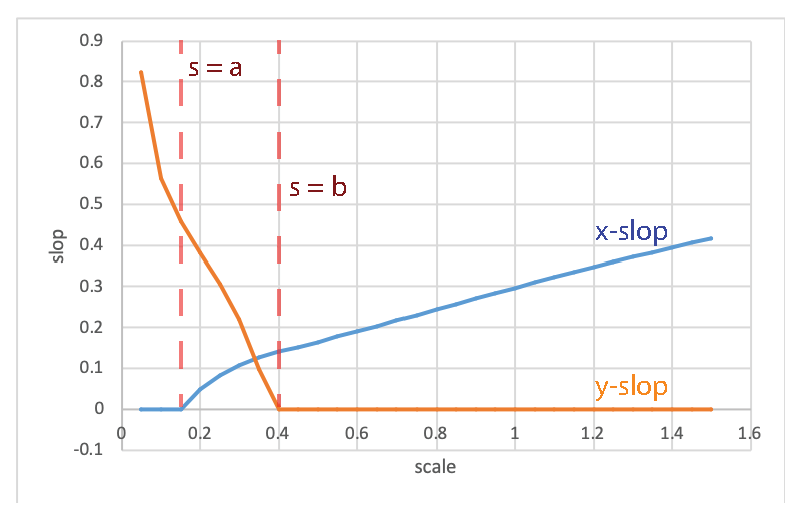
\includegraphics[width=0.8\linewidth]{figures/slopvscale.eps}
    \caption{Example of slop/extrinsic scatter $(\sigma_x,\sigma_y)$ dependence on fitting scale $s$ (for some linear model). Note that as is predicted in \S\ref{sec:TRKcorr}, there exist minimum and maximum scales $s=a$ and $s=b$ (respectively) such that $\lim\limits_{s\rightarrow a^+}\sigma_x = 0$ and $\lim\limits_{s\rightarrow b^-}\sigma_y = 0$.}
    \label{fig:slopvscale}
\end{figure}

In order to determine the scale extrema $a$ and $b$ for a given model and dataset, I implemented a type of bracketing/bisection method that, by running fits at various scales (using the Downhill Simplex routine of Algorithm \ref{algo:simplex}) and observing best fit slop values, finds the exact scales where the two slops go to zero. This method determines $a$ first, and then $b$; we present the method for determing $a$ as Algorithm \ref{algo:minscale}, and the similar method for determining $b$ is given as Algorithm \ref{algo:maxscale} in \S\ref{app:algos}. Note that I also make several modifications for improved efficiency, such as using best fit values for $\sigma_y$ obtained from determining $a$ to start the routine for determining $b$ at a better initial guess. I also provide the option to find the two scale extrema at the same time using parallel computing (in the current, C++ implementation of the TRK suite).
\begin{algorithm}
\label{algo:minscale}
\caption{Bracketing/Bisection-type method for determining minimum fitting scale $a$ for some model and dataset.}
\DontPrintSemicolon
    \SetKwInOut{Input}{Input}
    \SetKwInOut{Output}{Output}
    \SetKwProg{Fn}{Function}{}{}
    \Fn{FindMinimumScale}{
        \Input{Model $y_c$ and dataset $\{x_n,y_n\}$ with error bars $\{\sigma_{x,n}, \sigma_{y,n}\}$.}
        \Output{Minimum fitting scale $a$.}
        \Begin{
            \textit{Determine brackets $(l,r)$ for min scale $a$:}\;
            Initialize bisection brackets $l = s = 0, r = s = 1$ and $s_\text{trial} = s = 1$.\;
            $\sigma_x(s_\text{trial}) \leftarrow $\textit{ DownhillSimplex}($s=s_\text{trial}$)\;
            Initialize step modifier $\alpha = 0.5\times s_\text{trial}$.\;
            \If{$\sigma_x(s_\text{trial}) > 0$}{
                $r = s_\text{trial}$\;
                $l_\text{trial}=s_\text{trial}$\;
                $\sigma_x(l_\text{trial})=$\textit{DownhillSimplex}($s=l_\text{trial}$)\;
                \While{$\sigma_x(l_\text{trial}) > 0$}{
                    $l_\text{trial} = l_\text{trial}-\alpha$\;
                    $\sigma_x(l_\text{trial})=$\textit{DownhillSimplex}($s=l_\text{trial}$)\;
                    $\alpha = 0.5\times\alpha$\;
                    $r=l_\text{trial}$\;
                }
                $l=l_\text{trial}$\;
            }
            \ElseIf{$\sigma_x(s_\text{trial}) = 0$}{
                $l = s_\text{trial}$\;
                $r_\text{trial}=s_\text{trial}$\;
                $\sigma_x(l_\text{trial})=$\textit{DownhillSimplex}($s=l_\text{trial}$)\;
                \While{$\sigma_x(r_\text{trial}) = 0$}{
                    $r_\text{trial} = r_\text{trial}+\alpha$\;
                    $\sigma_x(r_\text{trial})=$\textit{DownhillSimplex}($s=r_\text{trial}$)\;
                    $l=r_\text{trial}$\;
                }
                $r=r_\text{trial}$\;
            }
            \textit{Use bisection to determine $a$ now that we have brackets $(l,r)$:}\;
            $a_\text{trial} = (l+r)/2$\;
            $\sigma_x(a_\text{trial})=$\textit{DownhillSimplex}($s=a_\text{trial}$)\;
            \While{$\abs{l-r}\geq$ tolerance1 AND $\sigma_x(a_\text{trial})\geq$ tolerance2}{
                $a_\text{trial} = (l+r)/2$\;
                $\sigma_x(a_\text{trial})=$\textit{DownhillSimplex}($s=a_\text{trial}$)\;
                \If{$\sigma_x(a_\text{trial})>0$}{
                    $r = a_\text{trial}$\;
                }
                \ElseIf{$\sigma_x(a_\text{trial})=0$}{
                    $l = a_\text{trial}$\;
                }
            }
            \Return{$a=a_\text{trial}$}
        }
    }
\end{algorithm}

Now that the method for determining the scale extrema $a$ and $b$ for a certain model and dataset has been presented, the optimum scale $s_0$ needs to be determined. From \S\ref{sec:TRKcorr}, in order to determine successive approximations for $s_0$ until convergence, Equation \eqref{eq:r2TRKnewscalenonlin} must be repeatedly solved for $s_0^{(2)}$ given the previous iteration's solution $s_0^{(1)}$. I begin this process with $s_0^{(1)}=(a+b)/2$, and then successively solve Equation \eqref{eq:r2TRKnewscalenonlin} numerically while setting $s_0^{(1)} = s_0^{(2)}$ after each iteration.

In practice, Equation \eqref{eq:r2TRKnewscalenonlin} is solved by rewriting it as
\begin{align}\label{eq:r2TRKnewscalenum}
\tilde{R}^2_{\mathrm{TRK}}(s_0^{(2)};s_0^{(1)}, a, b) & \equiv \frac{1}{N}\sum_{n=1}^{N}\tan^2\left(\frac{\pi}{4}-\frac{\left|\arctan  (s_0^{(1)}\tan\theta_{t,n;a})-\arctan  (s_0^{(1)}\tan\theta_{s_0^{(2)}})\right|}{2}\right) \nonumber \\
& -
\frac{1}{N}\sum_{n=1}^{N}\tan^2\left(\frac{\pi}{4}-\frac{\left|\arctan  (s_0^{(1)}\tan\theta_{s_0^{(2)}})-\arctan  (s_0^{(1)}\tan\theta_{t,n;b})\right|}{2}\right)\nonumber\\
& =0 \, ,
\end{align}
and numerically solving the equation for $s_0^{(2)}$ given the previous $s_0^{(1)} = s_0^{(2)}$ using a bisection root-finding routine, repeating as necessary until convergence\footnote{Here I use bisection instead of other root-finding algorithms (e.g. Newton-Raphson) because most of these other algorithms require derivatives of the function with respect to the independent variable. As the derivative of Equation \eqref{eq:r2TRKnewscalenum} with respect to $s_0^{(2)}$, for example, is ill-defined, the usage of bisection is a necessity. Furthermore, because this dependence of slop on scale has shown to be monatonic in all models that I have explored, bisection is perfectly suited for the task.}. We then set the final optimum scale $s_0$ to be the last iteration of $s_0^{(2)}$. This algorithm is presented in it's entirety as Algorithm \ref{algo:opscaler2} in \S\ref{app:algos}, on pg. \pageref{algo:opscaler2}.

\section{Model Parameter Distribution and Uncertainty Computation}
\subsection{Using Adaptive MCMC to Sample Parameter Distributions}
\label{sec:MCMC}
As a review, so far I have covered everything that is needed to determine best fit model and slop parameters for any given nonlinear model and dataset with intrinsic and extrinsic two-dimensional uncertainties. In practice, I run the scale optimization routine (Algorithms \ref{algo:minscale}, \ref{algo:maxscale}, and \ref{algo:opscaler2} sequentially) to determine the optimum fitting scale $s_0$, and then find the best fit model and slop parameters $\{\vartheta_m,(\sigma_x,\sigma_y)\}$ using the Nelder-Mead downhill simplex to maximize the TRK likelihood function $\mathcal{L}^\text{TRK}$ (Algorithm \ref{algo:simplex}). In reality, the \textit{uncertainties} of the best fit model parameters (and possibly the slop parameters) are also often desired as a result of a fit, if not their complete \textit{posterior} probability distributions \footnote{The latter often when the distribution(s) of the parameter are not simply Gaussian.}. Furthermore, if any prior information is known about the model parameters in the form of \textit{prior} probability distribution(s), it can be essential to introduce them to calculation of the posteriors, following Bayes' Theorem (Equation \eqref{eq:bayes}).

There are a number of methods that can be used to sample a parameter's (posterior probability) distribution, but the types of methods that offer some of the most flexibility, speed, and support for priors are  Markov Chain Monte Carlo, or \textit{MCMC} methods. MCMC methods are a class of algorithms used to sample probability distributions, and they fall under the broad umbrella of \textit{Monte Carlo Methods} which are, broadly speaking, the usage of the ability of computers to rapidly generate random numbers to simulate useful numerical results, that are often otherwise computationally intractable with more straight-forward methods. A simple example of a Monte Carlo method is the continuous sampling of a \textit{proposal} Gaussian distribution; as the number of samples becomes larger, the \textit{generated distribution} will converge to the proposal distribution. A \textit{Markov Chain} can generally be described as a process that continually changes from state to state following certain transition probability rules that are dependent on the previous state. Together, the moniker \textit{Markov Chain Monte Carlo} describes how a Markovian random walk is taken through parameter space to sample and generate the distribution of the parameters over time, according to chosen rules for the evolution and sampling. In turn, this sampling of the distribution can be used to estimate uncertainty, central tendency (e.g. mean, mode etc.), and other useful quantities. For the TRK algorithm suite, the specific MCMC method that we use is the classic Metropolis-Hastings sampling algorithm of \textcite{hastings1970monte}, which will be described as follows\footnote{I chose Metropolis-Hastings sampling over other methods, e.g. Hamiltonian Monte Carlo, due to it's speed, and because I have most model parameter distributions to well behaved enough for Metropolis-Hastings to be sufficient.}.

To begin, recall from \S\ref{sec:bayes} that the \textit{posterior probability distribution} of a model is the probability distribution of obtaining some values $\Theta\equiv\{\vartheta_m,(\sigma_x,\sigma_y)\}$ for the model (and slop) parameters given a dataset $D\equiv\{x_n,y_n,\sigma_{x,n},\sigma_{y,n}\}$. As such, in order to quantify any uncertainty of the predictions laid out by the best fit model parameters, the posteriors need to be examined. From Bayes' Theorem (Equation \eqref{eq:bayes}), then, sampling the posterior is \textit{equivalent} to (besides a factor of proportionality\footnote{Again, this constant factor is of no consequence because in most cases, we often don't care about the absolute probability of a some range of values for parameters, but rather the relative probability as compared to another range of possible values. Even if we did, we could integrate over the posterior to compute the constant of proportionality, as it is just a normalization constant found by the condition that $\int p(\Theta|D)\diff \Theta=1$.}) sampling the likelihood function multiplied by any priors\footnote{Note that if no priors are given for some or all of the parameters, the prior distribution(s) are \textit{uninformative}, or flat, i.e. $p(\Theta)=1$, such that the posterior is then directly proportional to the likelihood.}, i.e.
\begin{equation}
     P(\Theta|D)\propto\mathcal{L}^\text{TRK}(D|\Theta)p(\Theta)\,.
\end{equation}
Generally, the Metropolis-Hastings method works by iteratively generating a sequence of samples of parameters, that as the number of samples $R\rightarrow+\infty$, converges to the true probability distribution of the parameters. Given some sample $\Theta_i$, the possible distribution of the next potential sample $\Theta_t$, or the \textit{proposal distribution} $Q(\Theta_t|\Theta_i)$, is dependent on the value of $\Theta_i$ (which is why the sequence of samples is a Markov Chain). I note that by default, $Q$ is implemented as a Gaussian distribution, which could easily be changed if needed. The acceptance of this next potential sample is dependent on the proposal distribution: if it is accepted, it becomes the next step in the Markov Chain; if not, the sample is discarded and another potential sample is generated. The probability of acceptance for a potential parameter sample $\Theta_t$ is based off of the ratio between the posterior evaluated at the potential sample, and that at the previous sample $\Theta_i$; specifically, $\Theta_t$ is accepted if $\alpha \geq u$, where $\displaystyle\alpha\equiv \frac{\mathcal{L}^\text{TRK}(\Theta_t)p(\Theta_t)}{\mathcal{L}^\text{TRK}(\Theta_i)p(\Theta_i)}$ and $u\sim\mathcal{U}(0,1)$ ($\mathcal{U}$ indicates the uniform distribution)\footnote{\label{footnote:logpost}I note that in regions of parameter space that evaluate to extremely high likelihood, this ratio of posteriors $\displaystyle\frac{P(\Theta_t)}{P(\Theta_i)} = \frac{\mathcal{L}^\text{TRK}(\Theta_t)p(\Theta_t)}{\mathcal{L}^\text{TRK}(\Theta_i)p(\Theta_i)}$ can evaluate with underflow or overflow errors in practice. As such, in practice the TRK suite samples in log space, i.e. some trial $\Theta_t$ is accepted given a previous $\Theta_i$ if $\ln\alpha=\ln\mathcal{L}^\text{TRK}(\Theta_t) - \ln\mathcal{L}^\text{TRK}(\Theta_i) + \ln p(\Theta_t) - \ln p(\Theta_i)\geq \ln u$, where again $u\sim\mathcal{U}(0,1)$; this helps combat such numerical errors \textcite{stackoverflowlogpostsoln}. (Observing Equation \eqref{eq:TRK}, these errors can occur due to having large a dataset, small errorbars and/or slop, high or low datapoint weights---see footnote \ref{footnote:weighting} on page \pageref{footnote:weighting}---and/or other reasons.}.

The proposal distribution $Q(\Theta_t|\Theta_i)$ is proportional to the target \textit{true} posterior distribution $P(\Theta)$ (in our case we assume a Gaussian distribution for this, which can easily be changed), while the \textit{location} (i.e. mean) of $Q(\Theta_t|\Theta_i)$ is what changes from sample to sample (specifically, $Q(\Theta_t|\Theta_i)$ is centered on the most recent sample on the chain $\Theta_i$). The \textit{size}, or in other words the \textit{covariance matrix} $\Sigma$ and therefore standard deviations of $Q(\Theta_t|\Theta_i)$---the latter of which can be considered to be analogous to the step size(s) of the Markov Chain for each parameter, as will be shown shortly---on the other hand must be chosen prior to sampling, and will very much affect the quality and efficiency of the overall sampling. 

To see this behavior, consider some parameter $m$ that is Gaussian-distributed, that we wish to sample with the Metropolis-Hasting method. We need to choose the standard deviation/width $\sigma_m$ of the MCMC proposal distribution $Q(m)$ for the sampler, which we will refer to as the ``step size'' of the Markov Chain. We will use a fairly large sample count of $R=100,000$\footnote{Minus the ``burn-in'' of $10,000$ initial samples that are discarded, to allow for the Markov Chain to enter the majority of the distribution and not over-sample the outside.}, and run the sampler given three noticeably different values of $\sigma_m$. The results of these three separate samplings are shown in Figure \ref{fig:mcmcstepsize}; clearly, choosing the right values for the step sizes/proposal covariance matrix of an MCMC sampler is essential; step values that are too large or too small can lead to terrible samplings\footnote{The technical reasons for the erroneous nature of such samplings are beyond the scope of this work, but it is related to the  ratio of the number of potential samples accepted by the Metropolis-Hastings criterion to the number of total samples attempted. Too high a step size leads to too many samples being accepted, while too low a step size leads to too few. Initially, I attempted to optimize the $M+2$ step sizes of the model and slop parameters with respect to this acceptance ratio, but this proved faulty for a number of reasons.}.
\begin{figure}
    \centering
    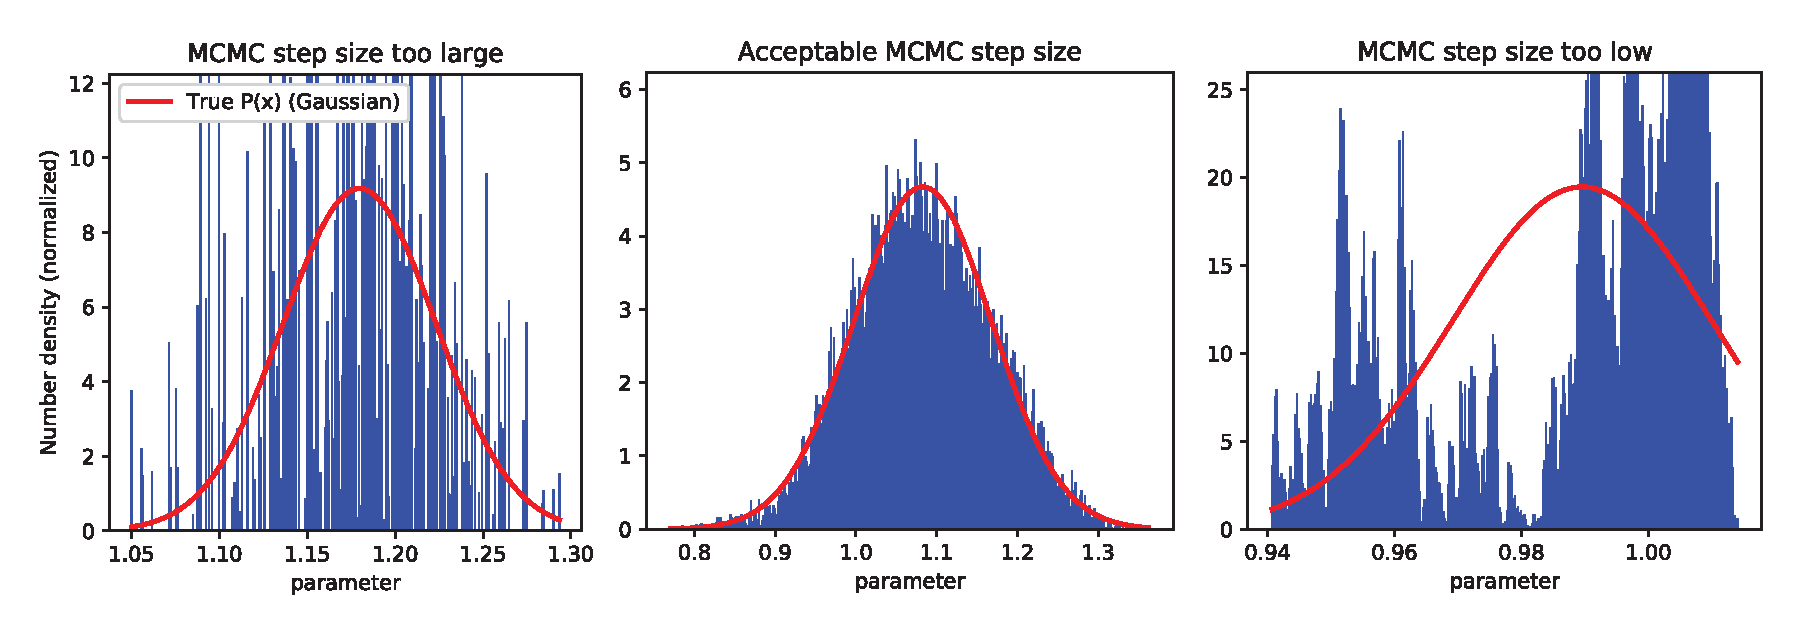
\includegraphics[width=1.0\linewidth]{figures/mcmcstepsizeall.eps}
    \caption{Histograms of MCMC Metropolis-Hastings samplings for a normal-distributed parameter $m$, with true Gaussian posterior plotted in red, given (Gaussian) proposal distribution widths/``step sizes'' of $\sigma_m=10$, $\sigma_m=0.1$, and $\sigma_m=0.0001$, from left to right, given a sample size of $R=100,000$. Note that even with such a high sample size, the choice of the step size for the model parameter's Markov Chain will \textit{drastically} change the quality of the sampling.}
    \label{fig:mcmcstepsize}
\end{figure}
However, it is very difficult to judge the quality of a choice of proposal distribution step sizes without running the full sampling itself. Because the TRK likelihood $\mathcal{L}^\text{TRK}$ requires running the tangent point-finding logic for all $N$ data-points at every evaluation of $\mathcal{L}^\text{TRK}$, and I have found that it usually takes $R\sim 100,000$ to get a decent sampling of the posterior, it requires $N\times 100,000$ calls to the tangent-point finding routine to sample the posterior distribution of the model and slop parameters of a given model and dataset. Even with parallelization and other optimizations, this requires a fair amount of computational work, especially if there are many datapoints and/or a complicated multi-dimensional model. As such, simply using trial-and-error to determine the best proposal distribution covariance matrix by iteratively running full samplings is computationally impractical, \textit{especially} if there are many model parameters, and therefore many step sizes that need tuning.

Because of this problem, I wished to efficiently automate the choosing of the proposal distribution covariance matrix, both to need as little user intervention and to require the lowest overall computation time as possible. To do so, I used the Adaptive MCMC algorithm of \textcite{haario2001adaptive}, which updates the (mean and covariance matrix of the) proposal distribution $Q$ while the sampling process is underway, according to the quality of the accumulating total sample. My implementation of the complete Adaptive MCMC sampler is shown as Algorithm \ref{algo:mcmc}.
\begin{algorithm}
\label{algo:mcmc}
\caption{Adaptive Metropolis-Hasting MCMC algorithm for sampling the posterior distribution of model and slop parameters.}
\DontPrintSemicolon
    \SetKwInOut{Input}{Input}
    \SetKwInOut{Output}{Output}
    \SetKwProg{Fn}{Function}{}{}
    \Fn{OptimizeMCMCProposalDist}{
        \Input{Optimum fitting scale $s=s_0$ (or any scale of choice), sample size $R$ ($100,000$ by default), ``burn-in'' count $B$ ($10,000$ by default), initial guess for $\mathcal{M}$ model and slop parameters/starting point for Markov chain $\Theta_g\equiv\{\vartheta_m,(\sigma_x,\sigma_y)\}_\text{guess}$, dataset $D\equiv\{x_n,y_n,\sigma_{x,n},\sigma_{y,n}\}$, and any parameter priors $p(\Theta)$.}
        \Output{$\{R$ samples of $\Theta$ from posterior, i.e. $\Theta\sim P(\Theta|D)\}$}
        \Begin{
        \textit{Notation: $\Sigma$, $\mu$ are the covariance matrix and mean vector of the proposal distribution $Q$, respectively, which is Gaussian by default.}\;
        Initialize guess $\Sigma_i$ for $\Sigma$ and $\mu_i=\Theta_g$ for $\mu$.\;
        \textit{Note: we use an automate the guessing of $\Sigma$, that can be fairly imprecise; however, this algorithm is very guess-independent, and we have never had issues with non-rapid convergence.}\;
        Initialize vector of all accepted samples as $S = \{\Theta_g\}$\;
        Initialize Markov Chain sampler starting point $\Theta_i=\Theta_g$ and define $\lambda=2.38^2/\mathcal{M}$\;
        \While{Sample count $\leq R + B$}{
            At iteration $i+1$:
            \textit{Sample trial $\Theta_t$ from posterior $P(\Theta)=\mathcal{L}^\text{TRK}(\Theta)p(\Theta)$ given current proposal $Q$ with Metropolis-Hastings acceptance criterion:}\;
            \While{$\Theta_t$ not accepted}{
                $\Theta_t \sim Q(\mu_i, \lambda\Sigma_i)$ \textit{(Gaussian by default)}\;
                $\displaystyle\alpha = \frac{P(\Theta_t)}{P(\Theta_i)} = \frac{\mathcal{L}^\text{TRK}(\Theta_t)p(\Theta_t)}{\mathcal{L}^\text{TRK}(\Theta_i)p(\Theta_i)}\quad$\textit{(See footnote \ref{footnote:logpost}.)}\;
                Accept $\Theta_t$ with probability $\min(1,\alpha)$
            }
            $\Theta_{i+1}=\Theta_t$\;
            Append $\Theta_{i+1}$ to $S$\;
            \textit{Update proposal $Q$:}\;
            $\gamma_{i+1}=1/(i+1)$\;
            $\mu_{i+1}=\mu_i+\gamma_{i+1}(\Theta_{i+1}-\mu_i)$\;
            $\Sigma_{i+1}=\Sigma_i+\gamma_{i+1}\left[(\Theta_{i+1}-\mu_i)(\Theta_{i+1}-\mu_i)^T-\Sigma_i\right]$
        }
        Remove first $B$ samples from $S$ (\textit{to account for burn-in})\;
        \Return{$S$}\;
        }
    }
\end{algorithm}

With the Metropolis Hastings and Adaptive MCMC methods, the posterior probability distribution(s) for the model and slop parameters of a model function can be generated, given some dataset and fitting scale. Given these distributions, we can now estimate the (Gaussian) uncertainties/standard deviations of the model parameters, using the following method.

\subsection{Computing Uncertainties from Parameter Distributions}
\label{sec:barlowering}
In order to estimate model parameter uncertainties/error bars given MCMC-sampled posterior distributions, the TRK suite uses what I refer to as the ``Bar-Lowering`` method from \textcite{trotter}. For some parameter, a $1-$, $2-$ or $3\sigma$ confidence interval corresponds to the range of possible parameter values that make up $68.27\%, 95.45\%$ and $99.73\%$ of the total integrated probability distribution, respectively. Given a model parameter sample distribution, this method works by first binning the samples into a histogram, and then iteratively finding exactly where $1\sigma, 2\sigma$ and $3\sigma$, i.e. $68.27\%, 95.45\%$ and $99.73\%$ of the data lies. This algorithm is explicitly given as Algorithm \ref{algo:barlower}.

\begin{algorithm}
\label{algo:barlower}
\caption{}
\DontPrintSemicolon
    \SetKwInOut{Input}{Input}
    \SetKwInOut{Output}{Output}
    \SetKwProg{Fn}{Function}{}{}
    \Fn{GetUncertainties}{
        \Input{MCMC-sampled model parameter distribution $S\equiv\{\{\vartheta_m\}\}$ and best fit parameters $\{\vartheta_m,(\sigma_x,\sigma_y)\}$.}
        \Output{$\pm1-$, $\pm2-$ and $\pm3\sigma$ confidence intervals/uncertainties of model parameters $\{\vartheta_m\}$.}
        \Begin{
            \For{each model parameter $\vartheta$}{
                    Make histogram of $\vartheta$ data from $S$, with $k$ bins total\;
                \For{all $n\sigma$ of $\pm1-$, $\pm2-$ and $\pm3\sigma$}{
                    Initialize brackets $h=\max$(bins in histogram), $l=0$\;
                    Initialize bar $b=h/2$\;
                    Let $r = $ (amount of histogram bins $\geq b$)/$k$\;
                    \While{$\abs{r-n\sigma}\geq$ tolerance}{
                        Update $r$\;
                        \If{$r < n\sigma$}{
                            $h = b$\;
                        }
                        \ElseIf{$r \geq n\sigma$}{
                            $l = b$\;
                        }
                        $b = (l + h) / 2$\;
                    }
                    
                    Let $-n\sigma = $ midpoint parameter value of leftmost bin above bar\;
                    Let $+n\sigma = $ midpoint parameter value of rightmost bin above bar\;
                }
            }
            \Return{$\{\pm1\sigma, \pm2\sigma, \pm3\sigma\text{ error bars } \forall \text{ model parameters }\{\vartheta_m\}\}$}
        }
    }
\end{algorithm}

Due to the binning nature of this algorithm, it also automatically computes the \textit{asymmetric} confidence intervals/standard deviations of parameters, i.e. $\pm1\sigma$, $\pm2\sigma$ and $\pm3\sigma$ intervals. For example, if the distribution of a parameter is a perfectly symmetric Gaussian, then the $-1\sigma$ width is equivalent to the $+1\sigma$ width, the $-2\sigma$ width is equivalent to the $+2\sigma$ width, etc. However, if the distribution is an \textit{asymmetric} Gaussian, e.g. Equation \eqref{eq:asymnorm} (see \S\ref{sec:asymm} for an in-depth discussion of such asymmetric distributions), all six different widths will be computed.

\subsection{Reality Check: A Linear TRK Example Fit}
\label{sec:linfitex}

At this point I have discussed all of the mechanisms for the basic functionality of the TRK algorithm suite. Before I delve into the advanced/additional topics of the following chapter, I will present a ``reality check'' of the TRK suite in the form of a basic linear fit. Consider the dataset shown in red in the top left of Figure \ref{fig:linfit}\footnote{The error bars are possibly too small to see; I choose these error bars to illustrate the fitting behavior for a slop-dominated dataset.}, and model of the functional form $y=mx+b$, i.e. model parameters of $b$ and $m$. Running a full TRK fit (i.e. scale optimization, likelihood maximization and then MCMC-generated uncertainty computation) resulted in the model distribution shown in the top left of Figure \ref{fig:linfit}. As expected, this slop-dominated dataset (i.e. the small error bars are not enough to account for the scatter of the data) resulted in a linear fit with high slop parameters $(\sigma_x, \sigma_y)$, as evidenced by the fairly large $1-$, $2-$ and $3\sigma$ confidence intervals of the model distribution shown\footnote{\label{footnote:modelcurvebands}These intervals are computed with the slop values and the model parameters, given some model. Specifically, the $n\sigma$ vertical offset of the interval boundaries are given by $\pm n\sqrt{\sigma_y^2 + \left(\dv{y_c(x)}{x}\sigma_x\right)^2}$, from \textcite{trotter}.}. After running this fit, I also show the results of the MCMC-generated model parameter distributions (the bottom of Figure \ref{fig:linfit}), including a confidence ellipse in parameter space with $1-$, $2-$ and $3\sigma$ regions shaded (top right of Figure \ref{fig:linfit}), generated via kernel density estimation.

% \begin{table}[h]
% \label{tbl:linfitdata}
% \centering
% \begin{tabular}{@{}lllll@{}}
% \toprule
% $x_n$ & $\sigma_{x,n}$ & $y_n$ & $\sigma_{y,n}$ & $w_n$ \\ \midrule
% 1.7   & 0.2            & 2.64  & 0.4            & 1     \\
% 2.1   & 0.2            & 3.59  & 0.4            & 1     \\
% 2.56  & 0.2            & 4.58  & 0.4            & 1     \\
% 5.65  & 0.2            & 4.53  & 0.4            & 1     \\
% 4.83  & 0.2            & 4.47  & 0.4            & 1     \\
% 6.56  & 0.2            & 7.28  & 0.4            & 1     \\
% 7.72  & 0.2            & 8.57  & 0.4            & 1     \\
% 8.28  & 0.2            & 8.74  & 0.4            & 1     \\
% 7.74  & 0.2            & 9.57  & 0.4            & 1     \\ \bottomrule
% \end{tabular}
% \caption{Data used for example linear fit shown in Fig. \ref{fig:linfit}}
% \end{table}

\begin{figure}
    \centering
    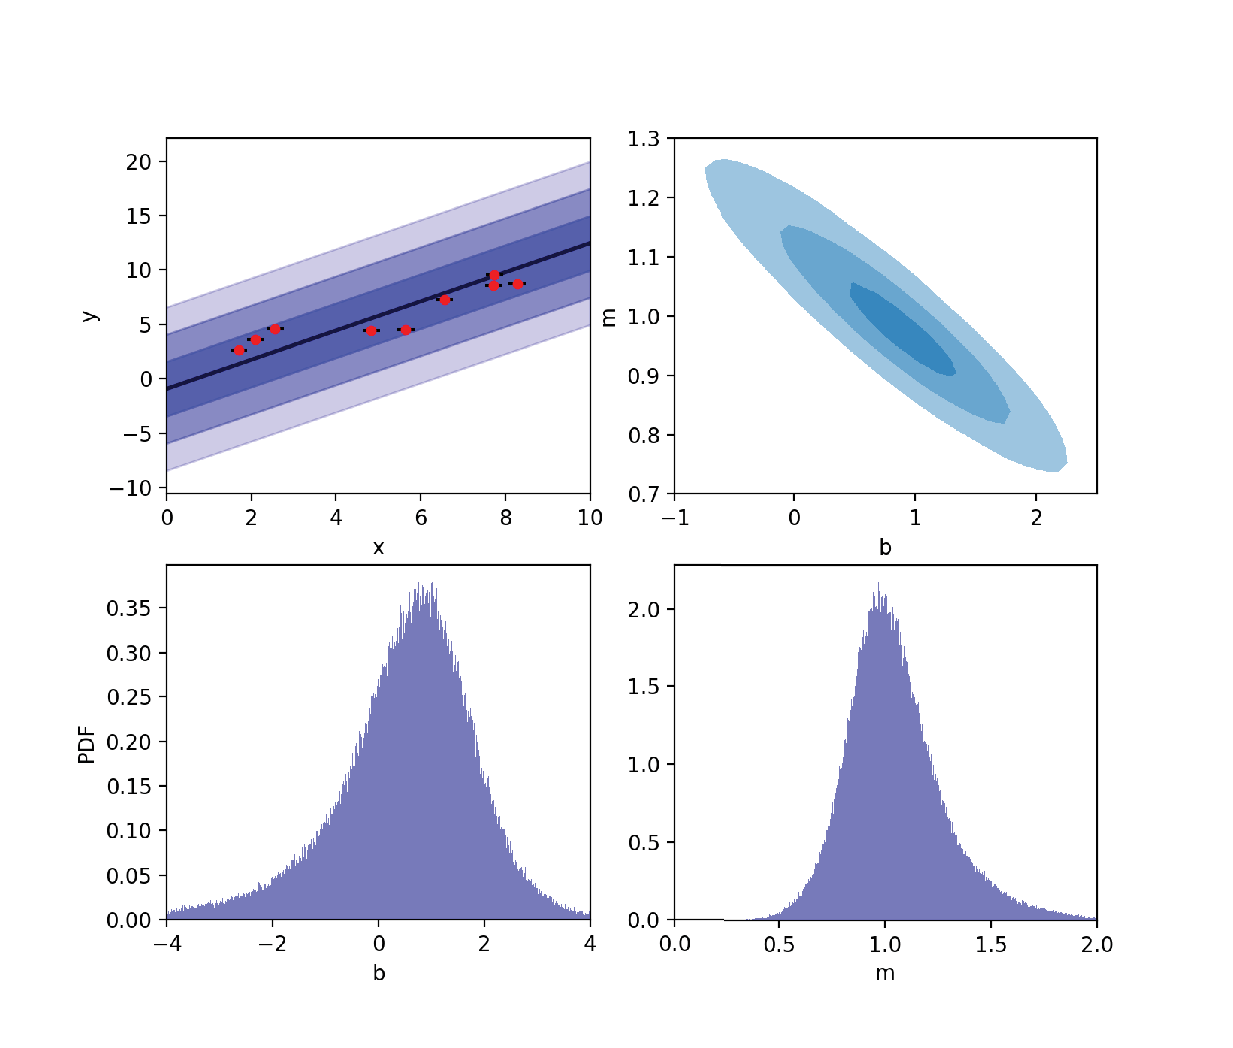
\includegraphics[width=1.0\linewidth]{figures/linfit_sloppy_3shadenoback.eps}
    \caption{Top left: Example extrinsic scatter-dominated dataset (red) with small $x-$ and $y-$ error bars (barely visible), alongside linear fit model distribution $y=mx+b$ with $1-$, $2-$ and $3\sigma$ slop confidence regions visible in blue. Top right: model parameter confidence ellipse with $1-$, $2-$ and $3\sigma$ regions shaded, generated from the posterior probability distributions for $b$ and $m$ found via MCMC, bottom.}
    \label{fig:linfit}
\end{figure}

I have now covered all of the essential parts of the TRK fitting suite, and provided an example of its usage. Before I  discuss the applications and more complicated examples of TRK fitting, and compare the algorithm to similar algorithms, I will first examine further algorithms and options of the TRK suite, including an automated algorithm for the minimization of model parameter correlation for certain models, and allowing for asymmetric error bars and/or slop parameters.            %% this is a suggestion: you have to create this file on demand
\chapter{The TRK Codebase: Additional Algorithms}
\label{cha:code2}
In the previous chapter I examined the basic usage of the TRK statistic to fit models to data, including fitting scale optimization, likelihood maximization, and model parameter probability distribution generation. These features are satisfactory for many fitting tasks, but more complicated situation may arise that require special, generalized treatment. In this chapter, I will first introduce an algorithm developed to remove correlation between model parameters. From here, I will then examine the more complicated, but general case of having asymmetric uncertainties, intrinsic and/or extrinsic, in a dataset, and how this can be fitted to as part of the TRK suite.

\section{Automatic Model Parameter Correlation Removal and Pivot Points}
\label{sec:pivot}
To begin, consider some linear model of the form $y=mx+b$; typically, the best-fit slop $m$ will be correlated with the best-fit intercept $b$, i.e. the confidence ellipse between the two parameters in parameter space will be tilted somewhat. This arises from the implicit choice of setting the intercept of the line at $x=0$; such a choice can create an effect where $m$ depends on the choice of $b$. Described as a ``lever-arm'' effect in \textcite{trotter}, this $x-$intercept choice mathematically corresponds to choosing some \textit{pivot point} $x_p$ for a model defined as $y=m(x-x_p)+b$. Choosing some $x_p$ will affect the best-fit $b$, which can in turn affect the best-fit $m$ to some degree. As shown in \textcite{trotter}, an optimal choice for $x_p$ exists such that the correlation of $b$ and $m$ is minimized (for some dataset).

\begin{figure}
    \centering
    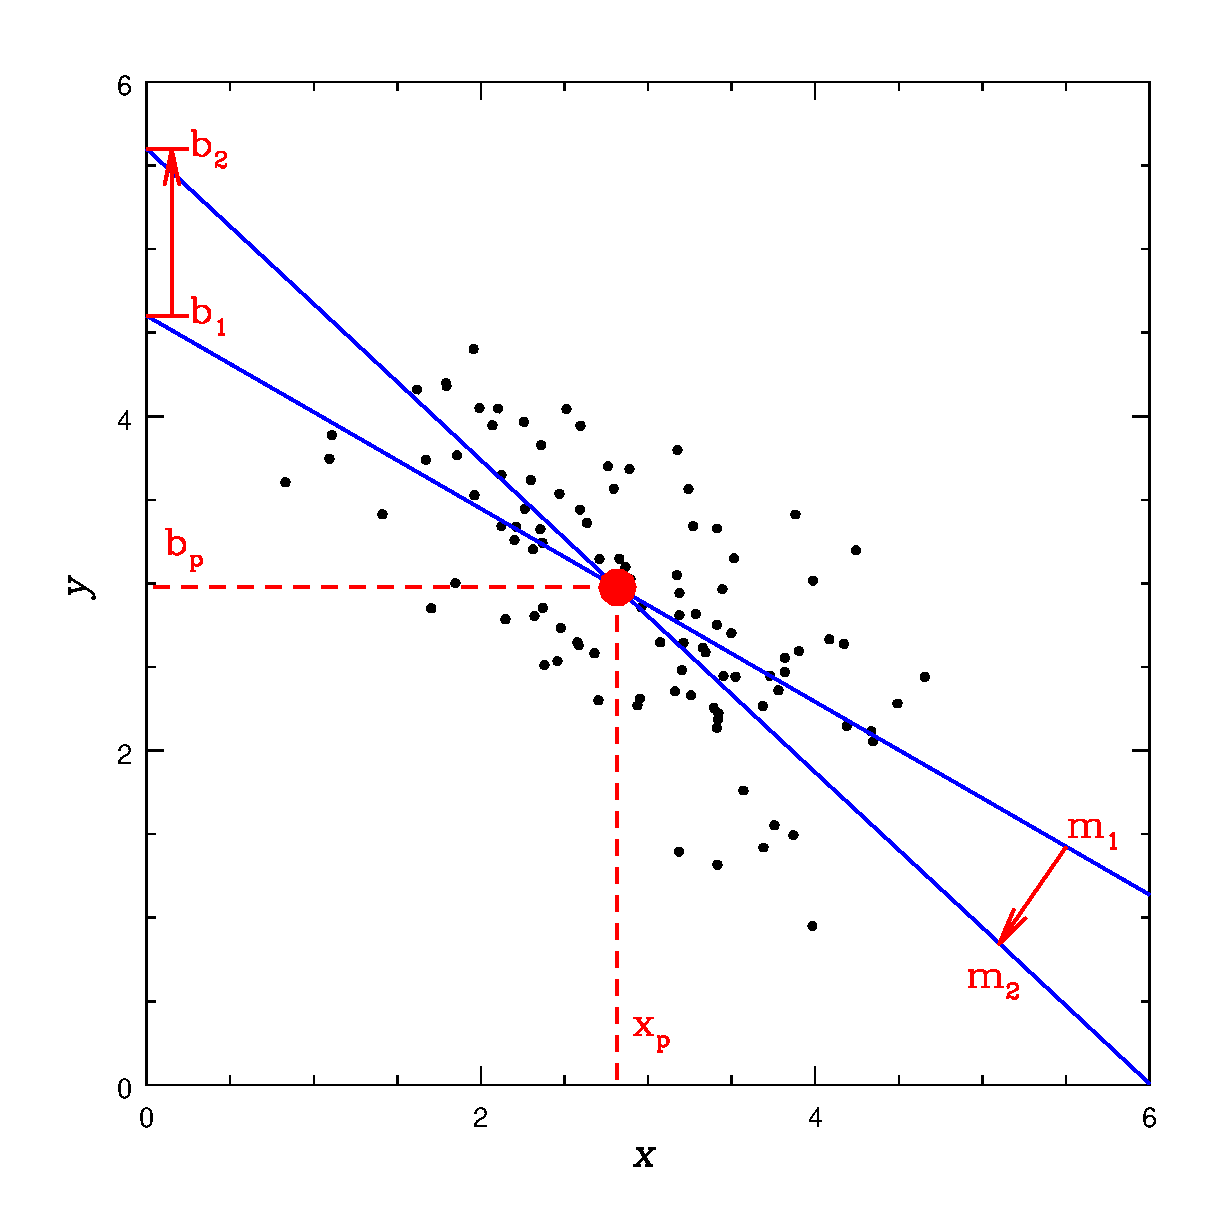
\includegraphics[width=0.8\linewidth]{figures/fig_pivot.eps}
    \caption{From \textcite{trotter}, this figure illustrates how two different choices of pivot point $x_p$ for the linear model $y=m(x-x_p)+b$ results in two different best-fit values for $b$, which in turn correlate to two different best-fit values for $m$. As shown, both of these lines intersect at some optimum pivot point $x_p$, plotted in red; if this optimal $x_p$ is chosen when fitting the model, the correlation between $b$ and $m$ will be minimized.}
    \label{fig:pivotpoint}
\end{figure}

We have devised an algorithm for automatically determining the pivot point for some model; I note that it can be used not just on linear models, but also any linearizable model, as long as the model can be (re-)written in the form of $y=m(x-x_p)+b$. As an example, consider the power-law model $\displaystyle y(x)=a_0\left(\frac{x}{10^{x_p}}\right)^{a_1}$. To linearize this, begin by taking the log of both sides as
\begin{equation}
\begin{split}
    \log_{10}y(x)&=\log_{10}\left[a_0\left(\frac{x}{10^{x_p}}\right)^{a_1}\right]=\log_{10}a_0 + \log_{10}\left(\frac{x}{10^{x_p}}\right)^{a_1}=\log_{10}a_0 + a_1\log_{10}\left(\frac{x}{10^{x_p}}\right)\\&= \log_{10}a_0 + a_1\left[\log_{10}x - \log_{10}10^{x_p}\right] = \log_{10}a_0 + a_1\left(\log_{10}x - x_p\right).
\end{split}
\end{equation}
As such, the linearized version of the power law has intercept $\log_{10}a_0\rightarrow b$, slope $a_1\rightarrow m$, and the data transforms as $\log_{10}y\rightarrow y$ and $\log_{10}x\rightarrow x$.

To introduce our correlation removal/pivot point-finding algorithm, begin by considering two linear (or linearized) fits 
\begin{equation}
\label{eq:2lines}
    y=m_1(x-x_p)+b_1 \qquad\text{and}\qquad y=m_2(x-x_p)+b_2
\end{equation}
with some shared pivot point $x_p$ (see Figure \ref{fig:pivotpoint}). To determine the \textit{optimum} pivot point, I take an iterative approach. As shown in Figure \ref{fig:pivotpoint}, the optimum pivot point should be the $x-$value where the two lines intersect; as such, we set Equations \eqref{eq:2lines} equal to each other and solve to obtain
\begin{equation}
    \label{eq:ppointeqn}
    x=x_p+ \frac{b_1-b_2}{m_2-m_1}.
\end{equation}

In order to use Equation \eqref{eq:ppointeqn} to solve for the optimum pivot point, we need two sets of slop and intercept parameters. However, what parameters should be used? Because no choice is known \textit{a priori},Ie take a Monte Carlo-based approach by using the Metropolis Hastings algorithm (Algorithm \ref{algo:mcmc}) to generate a large sampling (e.g. $R\sim 10,000$) of intercept and slope parameters $(b,m)$, given some previous iteration (or guess, if on the first iteration) of the pivot point $x_p=x_p^\text{old}$. I then generate $K\sim 100,000$ randomly-drawn 2-combinations of pairs of $(b,m)$ from this sample (i.e. various $\{(b_1,m_1),(b_2,m_2)\}$ of Equation \eqref{eq:ppointeqn})\footnote{I note that although I don't use explicit mechanisms to avoid duplicate 2-combinations, there are $\binom{10,000}{2} \simeq 5\times 10^7$ possible randomly-chosen 2-combinations from the set of $10,000$ samples, so if $100,000$ are combinations drawn, there is only a $\simeq 0.2\%$ chance of having a single duplicate.}. From this, I compute $100,000$ possible new pivot points $x_p^\text{new}$ using Equation \eqref{eq:ppointeqn}. From here, how can we use this \textit{distribution} of $x_p^\text{new}$ to determine the optimal $x_p^\text{new}$, i.e. the next iteration of the true optimal pivot point that will minimize correlation?

To start, I desired to choose a weight $w_{x_p^\text{new}}$ for each value of $x_p^\text{new}$ according to the uncertainty $\sigma_{x_p^\text{new}}$ of it's computation, i.e. $w_{x_p^\text{new}}=1/\sigma_{x_p^\text{new}}^2$, given the $\{(b_1,m_1),(b_2,m_2)\}$ that were used to compute it\footnote{This relationship between weight and uncertainty assumes (approximately) Gaussian error.}. To do so, I used standard propagation of uncertainty to first linear order with Equation \eqref{eq:ppointeqn} to obtain
\begin{equation}
\label{eq:ppointweight1}
\sigma_{x_p^\text{new}} \simeq \sqrt{2\left(\frac{\sigma_b}{m_2-m_1}\right)^2 + 2\left[\frac{b_1-b_2}{(m_2-m_1)^2}\right]^2\sigma_m^2}\,,
\end{equation}
where I've assume that the uncertainties $\sigma_{b_1}=\sigma_{b_2}\equiv\sigma_b$ and $\sigma_{m_1}=\sigma_{m_2}\equiv\sigma_m$. Next, note that for a linear model $y=m(x-x_p)+b\equiv mx^\prime+b$, we have that $\sigma_b^2=\sigma_m^2\overline{(x^\prime)^2}=\sigma_m^2\overline{(x-x_p)^2}$, where the overline indicates an average over all $N$ datapoints (\textcite{morrison2014obtaining}). Combining this with Equation \eqref{eq:ppointweight1}, we now have that 
\begin{equation}
\label{eq:ppointweight2}
\sigma_{x_p^\text{new}} \simeq \sqrt{2\frac{\sigma_m^2\overline{(x-x_p)^2}}{(m_2-m_1)^2} + 2\frac{(b_1-b_2)^2}{(m_2-m_1)^4}\sigma_m^2}=\sqrt{2}\sigma_m\sqrt{\frac{\overline{(x-x_p)^2}}{(m_2-m_1)^2} + \frac{(b_1-b_2)^2}{(m_2-m_1)^4}}\,.
\end{equation}

Given that each $x_p^\text{new}$ can be weighted according to $w_{x_p^\text{new}}=1/\sigma_{x_p^\text{new}}^2$, we can factor out constants of proportionality in Equation \eqref{eq:ppointweight2} to obtain
\begin{equation}
w_{x_p^\text{new}} \propto \left[\frac{\overline{(x-x_p)^2}}{(m_2-m_1)^2} + \frac{(b_1-b_2)^2}{(m_2-m_1)^4}\right]^{-1}\,.
\end{equation}
Finally, note that for our iterative approach, $x$ ranges over the sample of the $K=100,000$ new pivot points $x_p^\text{new}$ computed from Equation \eqref{eq:ppointeqn}, and $x_p$ is the previous iteration's optimal single pivot point $x_p^\text{old}$. As such, a single $i^\text{th}$ new pivot point $x_{p,i}^\text{new}$ computed using some $\{(b_1,m_1),(b_2,m_2)\}$ with Equation \eqref{eq:ppointeqn} is weighted according to 
\begin{align}
\label{eq:ppointweight}
w_{x_{p,i}^\text{new}} &\propto\displaystyle \left[\frac{\sum_{j=1}^{K}\left[\left(x_p^\text{old}+ \frac{b_{1,j}-b_{2,j}}{m_{2,j}-m_{1,j}}\right)-x_p^\text{old}\right]^2}{K(m_2-m_1)^2} + \frac{(b_1-b_2)^2}{(m_2-m_1)^4}\right]^{-1} \nonumber \\
&=\displaystyle\left[\frac{\sum_{j=1}^{K}\left(\frac{b_{1,j}-b_{2,j}}{m_{2,j}-m_{1,j}}\right)^2}{K(m_2-m_1)^2} + \frac{(b_1-b_2)^2}{(m_2-m_1)^4}\right]^{-1}\,,
\end{align}
which is the final expression that is used. Finally, I take the weighted half-sample mode (i.e. \textcite{bickel2005fast}) of the $K=100,000$ values for $x_p^\text{new}$ weighted according to Equation \eqref{eq:ppointweight}, and use that as the next iteration for the optimum $x_p$. From here, I iterate until convergence.

\begin{figure}
    \centering
    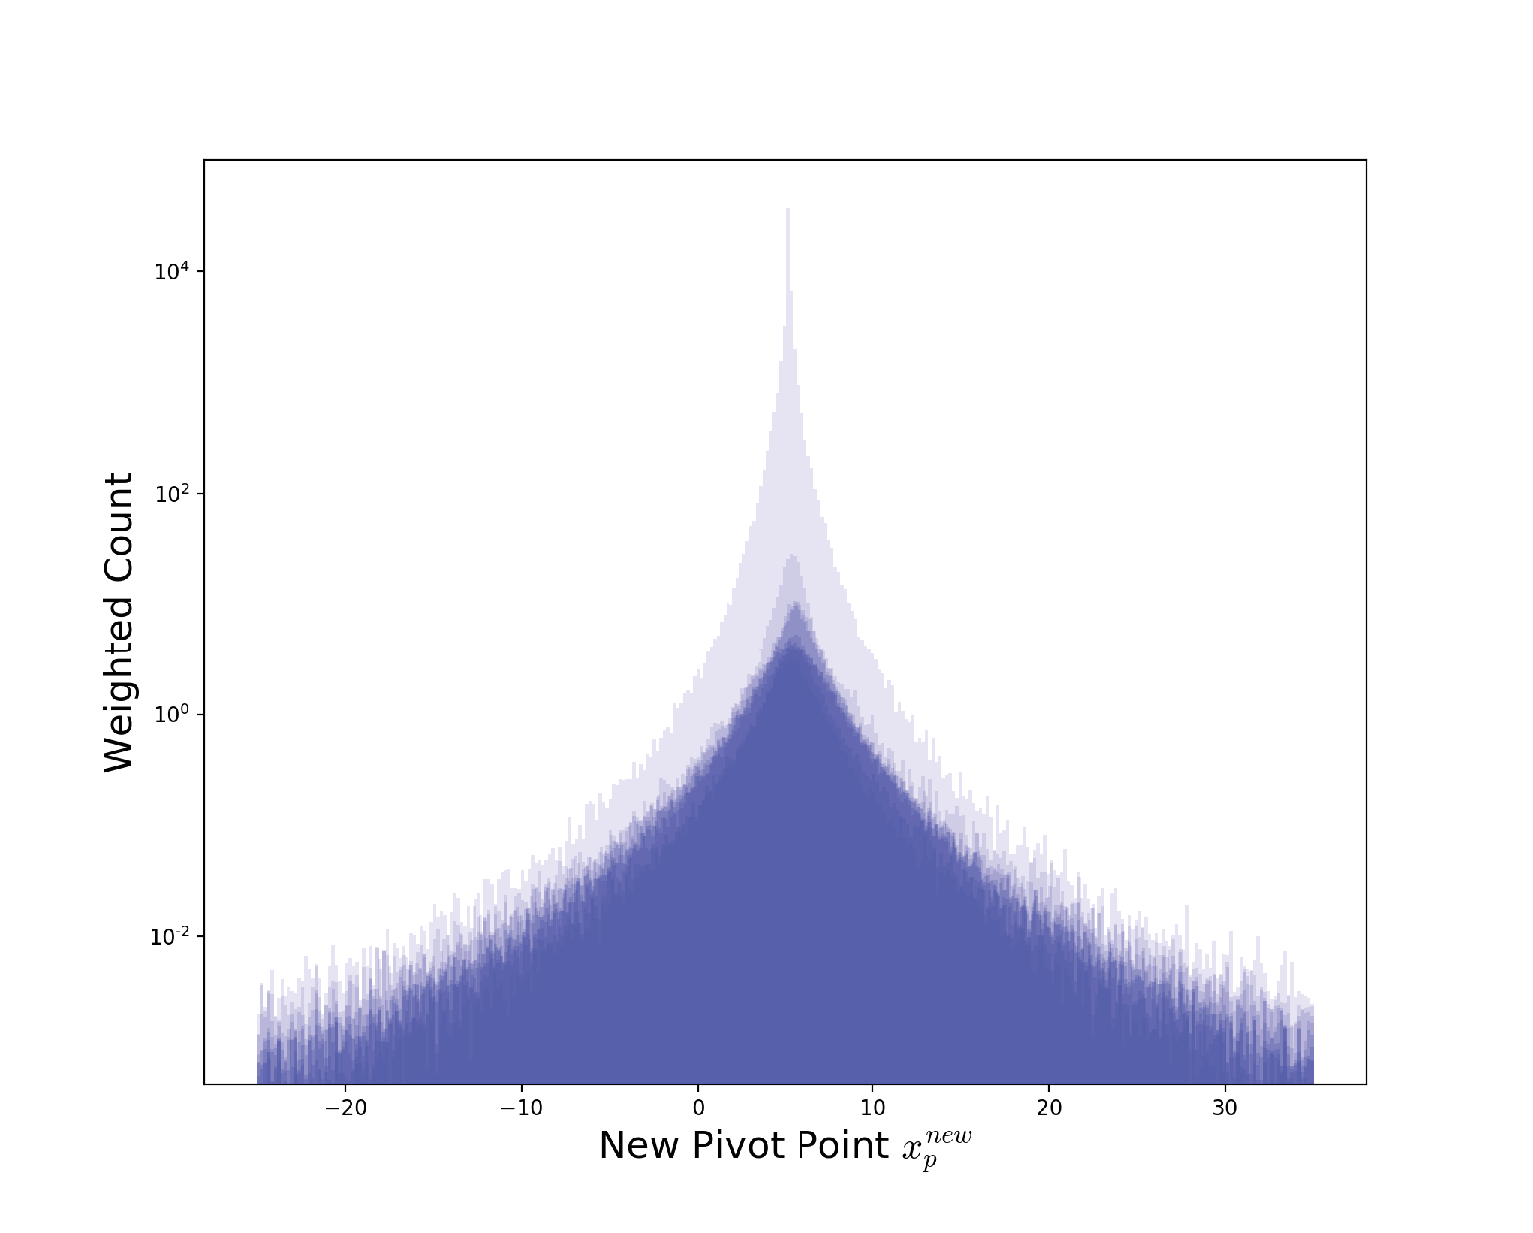
\includegraphics[width=0.8\linewidth]{figures/pivotpointdist.eps}
    \caption{Ten different iterations for the MCMC-generated distributions of new pivot points $x_p^\text{new}$ computed with Equation \eqref{eq:ppointeqn} and weighted according to Equation \eqref{eq:ppointweight}, overlapped. For each iteration we take the optimal value of the new pivot point to be the weighted half-sample mode (see \textcite{bickel2005fast}) of that iteration's distribution, and use this optimal value as $x_p^\text{old}$ for the next iteration in order to compute the next distribution of $x_p^\text{new}$.}
    \label{fig:ppointiters}
\end{figure}

I summarize the pivot point-finding/correlation removal method in Algorithm \ref{algo:pivotpoint}. Once the final pivot point has been found, it is stored as part of the model, and the rest of the TRK algorithm can be used as normal. As an example of this method, in Fig. \ref{fig:linfitnocorr} I show the results of running the pivot point optimization algorithm on the same linear fit dataset as in Figure \ref{fig:linfit} of \S\ref{sec:linfitex}, then running the regular TRK scale optimization, fit and MCMC uncertainty computation as usual. Observe in this figure how the best-fit slope $m$ is mostly unchanged from Figure \ref{fig:linfit}, but the intercept $b$ is noticeably different. Most notably, the parameter space confidence ellipse of $b$ and $m$ is no longer tilted, indicating a loss of correlation between the two parameters. Quantifiably, note that for the fit in Figure \ref{fig:linfit} where the pivot point was not optimized beforehand, the sampled $(b,m)$ has a Pearson correlation coefficient of $R^2 = -0.502$, indicating (negative) correlation as expected. On the other hand, when the pivot point \textit{is} optimized before running this fit, shown in Fig. \ref{fig:linfitnocorr}, the same correlation coefficient is only $R^2=0.056\simeq 0$, indicating almost no correlation, as expected.

\begin{algorithm}
\label{algo:pivotpoint}
\caption{Method to remove model parameter correlation/determine pivot point for linearized models}
\DontPrintSemicolon
    \SetKwInOut{Input}{Input}
    \SetKwInOut{Output}{Output}
    \SetKwProg{Fn}{Function}{}{}
    \Fn{FindPivotPoint}{
        \Input{Linearized model of the form $y_c(x)=m(x-x_p)+b$, dataset $D\equiv\{x_n,y_n,\sigma_{x,n},\sigma_{y,n}\}$, and initial guess for optimum pivot point $x_p^\text{old}$.}
        \Output{Optimum pivot point $x_p$ that minimizes correlation between model parameters $b$ and $m$.}
        \Begin{
        Initialize $R=10,000, K=100,000$ (by default)\;
        \While{$x_p^\text{new}$ not converged}{
            Initialize empty arrays $\mathcal{X}$, $\mathcal{W}$ for new pivot points and their weights, respectively\;
            Generate $R$ samples of $(b,m)\sim MetHastSampler()$(see Algorithm \ref{algo:mcmc})\;
            Store these samples as the set $\mathcal{P}$\;
            \textit{Compute $K$ new pivot points:}\;
            \For{$i=1,2,\cdots,K$}{
                Randomly draw pair $\{(b_1,m_1),(b_2,m_2)\}$. from $\mathcal{P}$\;
                Let $x_{p,i}^\text{new}=x_p^{old} + \frac{b_1-b_2}{m_2-m_1}$\;
                Store $x_{p,i}^\text{new}$ in $\mathcal{X}$\;
            }
            \textit{Weight these $K$ new pivot points:}\;
            \For{$i=1,2,\cdots,K$}{
                Let weight $w_{x_{p,i}^\text{new}} =\displaystyle\left[\frac{\sum_{j=1}^{K}\left(\frac{b_{1,j}-b_{2,j}}{m_{2,j}-m_{1,j}}\right)^2}{K(m_2-m_1)^2} + \frac{(b_1-b_2)^2}{(m_2-m_1)^4}\right]^{-1}$\;
                Store $w_{x_{p,i}^\text{new}}$ in $\mathcal{W}$\;
            }
            Compute optimum $x_p^\text{new}=WeightedHalfSampleMode(\mathcal{X},\mathcal{W})$\;
            $x_p^\text{new}\rightarrow x_p^\text{old}$\;
        }
        }
        \Return{$x_p = x_p^\text{new}$}
    }
\end{algorithm}


\begin{figure}
    \centering
    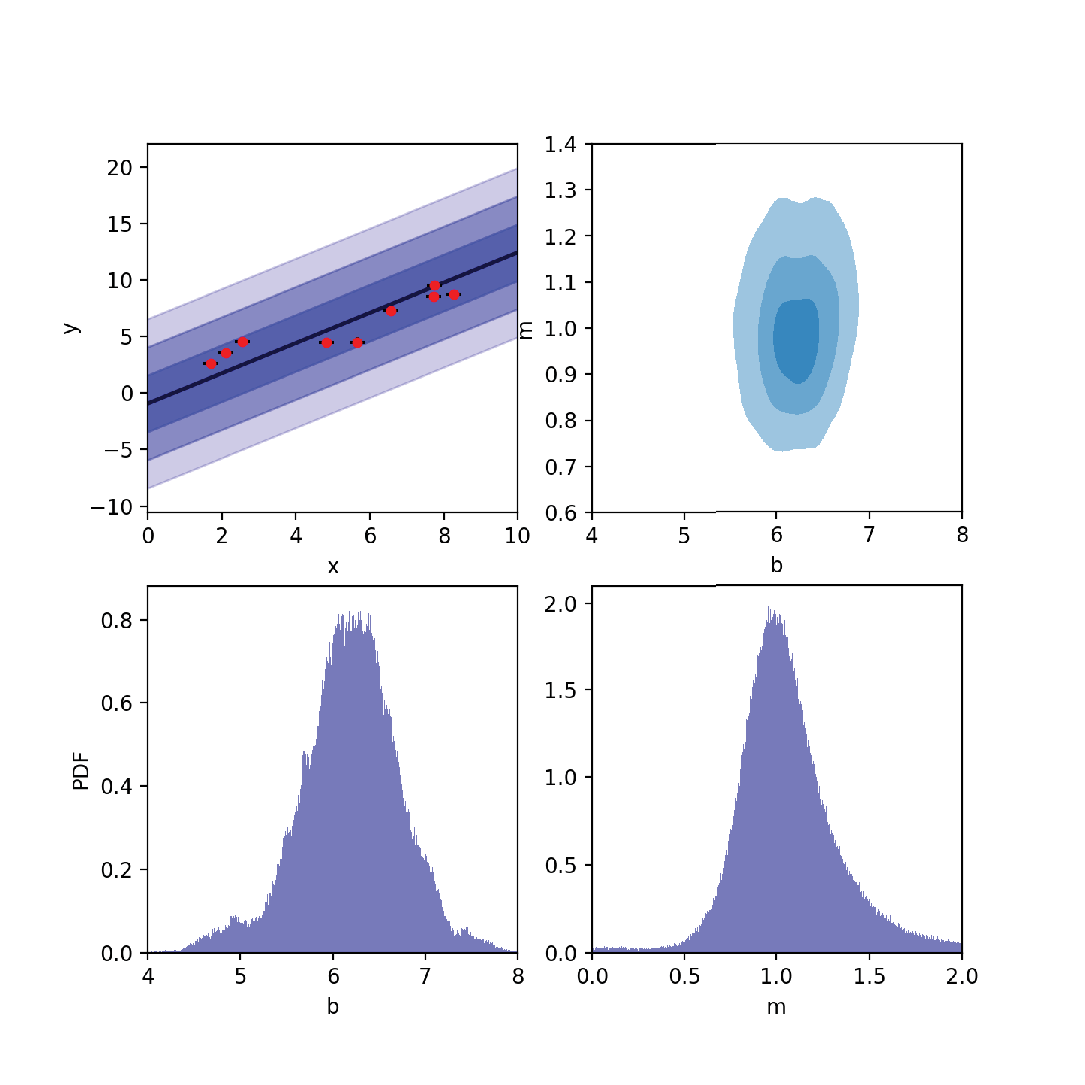
\includegraphics[width=1.0\linewidth]{figures/linfit_sloppy_3shadenoback_pivot.eps}
    \caption{Top left: The same extrinsic scatter-dominated dataset as in Figure \ref{fig:linfit} but now with pivot point $x_p$ in model $y=m(x-x_p)+b$ optimized to minimize correlation between $b$ and $m$, using Algorithm \ref{algo:pivotpoint}. Model is shown with $1-$, $2-$ and $3\sigma$ slop confidence regions visible in blue. Top right: model parameter confidence ellipse with $1-$, $2-$ and $3\sigma$ regions shaded, generated from the posterior probability distributions for $b$ and $m$ found via MCMC, bottom. Note that with pivot point optimized, the confidence ellipse is now no longer tilted as in Fig. \ref{fig:linfit}, indicating the removal of correlation, also evidenced by a Pearson correlation coefficient of $R^2=0.056\simeq 0$.}
    \label{fig:linfitnocorr}
\end{figure}

The ability to minimize parameter correlation for linearized models is a useful and widely applicable addition to the TRK suite. Next, in order to further generalize the TRK statistic, I will explore the possibility of introducing asymmetric error bars and/or slop parameters.

\section{Asymmetric Intrinsic and/or Extrinsic Uncertainty}
\label{sec:asymm}
Throughout this thesis I have only considered models that have intrinsic and extrinsic scatter (i.e. error bars and slop, respectively) that follow \textit{symmetric} Gaussian distributions, i.e. Equation \eqref{eq:symnorm}. However, there remains the distinct possibility for either or both the error bars and the slop/extrinsic scatter to follow \textit{asymmetric} distributions, such as the skew-normal distribution. A number of examples of asymmetric error bars within datasets and/or asymmetric slop within models are given in \textcite{trotter}, and as shown in that work, an excellent approximation of such distributions is defined as the (normalized) \textit{asymmetric} Gaussian distribution,
\begin{equation}
\label{eq:asymnorm}
\mathcal{N}_A(x^\prime;\mu,\sigma_{+},\sigma_-) \equiv \frac{2}{\sqrt{2\pi}(\sigma_{+} +\sigma_{-})} \left\{ \begin{array} {lr}
\exp{\left[-\frac{1}{2}\left(\frac{x^\prime-\mu}{\sigma_{+}}\right)^2\right]}\,\, \mbox{if $x^\prime\geq \mu$} \\
\exp{\left[-\frac{1}{2}\left(\frac{x^\prime-\mu}{\sigma_{-}}\right)^2\right]}\,\, \mbox{if $x^\prime < \mu$} \end{array} \right. \, .
\end{equation}
From here, a 2D asymmetric Gaussian is simply the product of two of these 1D asymmetric Gaussians. Note that this is just a general case of the typical symmetric Gaussian, as this expression simplifies to Equation \eqref{eq:symnorm} when $\sigma_-=\sigma_+\equiv\sigma$.
In the next section, following the work of \textcite{trotter}, I will show how this distribution can be introduced to the TRK statistic in the form of both asymmetric error bars and/or slop.

\subsection{Theory}
I will first introduce some notation. Following \textcite{trotter}, I parameterize the asymmetric $x$ and $y$ error bars of some $n^\text{th}$ datapoint with some parameters $\{\sigma_{x,n+},\sigma_{x,n-}\}$ and $\{\sigma_{y,n+},\sigma_{y,n-}\}$, respectively, following Equation \eqref{eq:asymnorm}. If asymmetric slop/extrinsic scatter along $x$ and/or $y$ is also modeled, such asymmetry is characterize with parameters $\{\sigma_{x+},\sigma_{x-}\}$ and $\{\sigma_{y+},\sigma_{y-}\}$, respectively. Now, in order to perform TRK fits on asymmetric data and/or models, because I have fundamentally generalized the concept of intrinsic and extrinsic scatter, the TRK statistic must be re-developed following the analysis of \S\ref{cha:TRK} with this new asymmetric formalism. To begin, consider a model distribution about the model curve $y_c(x;\vartheta_m)$ that has asymmetric Gaussian slops $(\sigma_{x\pm},\sigma_{y\pm})$, alongside a single $n^\text{th}$ datapoint with asymmetric Gaussian error bars $(\sigma_{x,n\pm},\sigma_{y,n\pm})$, illustrated in Figure \ref{fig:asymm}. Delving into this section, observe that the joint probability of this data-point $p_n$ requires evaluating the convolution of the two asymmetric Gaussians defined by $(\sigma_{x\pm},\sigma_{y\pm})$ and $(\sigma_{x,n\pm},\sigma_{y,n\pm})$, according to Equation \ref{eq:pn}. 

\begin{figure}
    \centering
    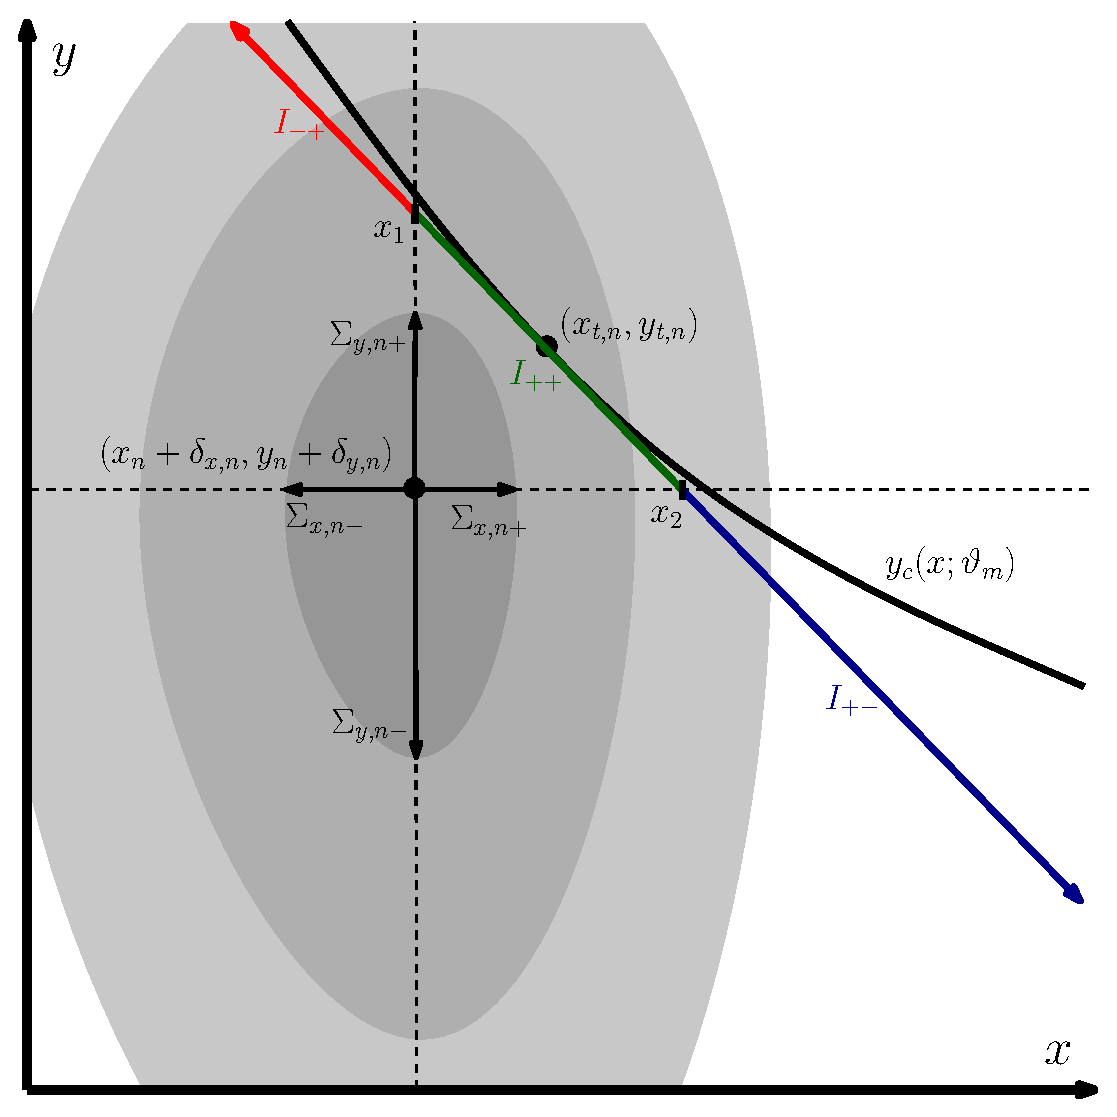
\includegraphics[width=0.8\linewidth]{figures/dia_asymint.eps}
    \caption{From \textcite{trotter}, a visualization of the 2D joint probability for an asymmetric model curve $y_c$ and data-point $(x_n,y_n)$ with asymmetric error bars. This joint probability is an integral that can be approximated by a 2D asymmetric Gaussian with widths $(\Sigma_{x,n\pm}, \Sigma_{y,n\pm})$ centered at some $(x_n+\delta_{x,n}, y_n+\delta_{y,n})$. The integral is broken into three segments according to the quadrants about the convolved centroid $(x_n+\delta_{x,n}, y_n+\delta_{y,n})$, in this case $I_{-+}$, $I_{++}$ and $I_{+-}$, respectively, with subscripts denoting which quadrant the integral/linear approximation of the model curve is located in. For this example, $I_{-+}$ (red) through quadrant 2 has limits $(-\infty,x_1]$, $I_{++}$ (green) through quadrant 1 has limits $[x_1,x_2]$, and $I_{+-}$ (blue) through quadrant 4 has limits $[x_2,\infty)$.}
    \label{fig:asymm}
\end{figure}

As shown in \textcite{trotter}, the convolution of two asymmetric Gaussian distributions does not itself exactly result in an asymmetric Gaussian. However, Trotter showed that an excellent approximation of such a convolution is a 2D asymmetric Gaussian with widths defined by $(\Sigma_{x,n\pm}, \Sigma_{y,n\pm})$ and centroid defined by $(x_n+\delta_{x,n}, y_n+\delta_{y,n})$, where
\begin{align}\label{eq:bigsigsasym}
\Sigma_{x,n\pm} & \equiv \left(\sigma_{x\mp}^2 + \sigma_{x,n\pm}^2\right)^{1/2} \nonumber\\
\Sigma_{y,n\pm} & \equiv \left(\sigma_{y\mp}^2 + \sigma_{x,n\pm}^2\right)^{1/2} \,
\end{align}
and $(\delta_{x,n},\delta_{y,n})$ describes an offset from the data-point which can be found using an empirical method developed by Trotter, given in Algorithm \ref{algo:asymmshifts}, of which the derivation of is beyond the scope of this work. Given that the likelihood is the product of all $N$ of the joint probabilities of the datapoints, using this 2D asymmetric Gaussian approximation for the integral in Equation \eqref{eq:pn} used to compute $p_n$ gives rise to an interesting observation. From \textcite{trotter}, in this asymmetric case the likelihood will have the form of a $\chi^2$-like statistic, but with the datapoint shifted from $(x_n,y_n)$ by $(\delta_{x,n},\delta_{y,n})$, with $\pm1\sigma$ error bars expanded in quadrature by the $\pm$-components of the model slop.

\begin{algorithm}
\label{algo:asymmshifts}
\caption{Method from \textcite{trotter} used to determine offsets $(\delta_{x,n},\delta_{y,n})$ from data-point $(x_n,y_n)$ that are used to compute the 2D asymmetric Gaussian joint probability distribution for some $n^\text{th}$ data-point.}
\DontPrintSemicolon
    \SetKwInOut{Input}{Input}
    \SetKwInOut{Output}{Output}
    \SetKwProg{Fn}{Function}{}{}
    \Fn{GetAsymmShifts}{
        \Input{Asymmetric slop parameters $(\sigma_{x\pm},\sigma_{y\pm})$ and asymmetric error bars $(\sigma_{x,n\pm},\sigma_{y,n\pm})$}
        \Output{Offset $(\delta_{x,n},\delta_{y,n})$}
        \Begin{
        Initialize $\sigma_{L}\equiv\mathrm{max}\left\{\sigma_{y+},\sigma_{y-}\right\}$, $\sigma_{S}\equiv\mathrm{min}\left\{\sigma_{y+},\sigma_{y-}\right\}$,\; $\sigma_{n,L}\equiv\mathrm{max}\left\{\sigma_{y,n+},\sigma_{y,n-}\right\}$,
        $\sigma_{n,S}\equiv\mathrm{min}\left\{\sigma_{y,n+},\sigma_{y,n-}\right\}$, and\; $\sigma_{\mathrm{max}}\equiv\mathrm{max}\left\{\sigma_{L},\sigma_{n,L}\right\}$.\;
        Let $\xi\equiv\frac{\sigma_S}{\sigma_L}+\frac{\sigma_{n,S}}{\sigma_{n,L}}$ and $\eta\equiv \left\{ 
        \begin{array} {lr}
        \frac{\sigma_{n,S}}{\sigma_{n,L}}-\frac{\sigma_{S}}{\sigma_{L}} & \,\,\mbox{if $\sigma_{n,L} < \sigma_{L}$} \, \\
        \frac{\sigma_{S}}{\sigma_{L}}-\frac{\sigma_{n,S}}{\sigma_{n,L}} & \,\,\mbox{if $\sigma_{n,L} \geq \sigma_{L}$} \, .
        \end{array} \right.$\;
        Define $r \equiv \frac{\mathrm{min}\left\{\sigma_{L},\sigma_{n,L}\right\}}{\mathrm{max}\left\{\sigma_{L},\sigma_{n,L}\right\}}$, $\xi^{\prime} = \left\{ \begin{array} {lr}
        \xi & \,\,\mbox{if $\xi\leq 1$}\, \\
        2-\xi & \,\,\mbox{if $\xi > 1$}\, \\
        \end{array} \right.$ and\;
        \vspace{0.3cm}$\eta^{\prime} = \left\{ \begin{array} {lr}
        0 & \,\,\mbox{if $\xi^{\prime} = 0$}\, \\
        2\xi^{\prime}\left[\frac{1}{2}\frac{\eta}{\xi^{\prime}}+1\right]^{n(r)}-\xi^{\prime} & \mbox{otherwise} \,
        \end{array} \right.$, where $n(r) \equiv r^{-0.4087}$.\;
        Compute $\delta_{\ast} = \sigma_{\mathrm{max}}N(r)\left[f(\xi)g(\eta^{\prime})+h(\xi)\right]$, given $N, f, g$ and $h$:\;
        \begin{eqnarray}
        N(r) & = & -0.5326r^2+1.5307r + 0.0019 \\
        f(\xi) & = & \left\{ \begin{array} {lr}
        0 & \,\,\mbox{if $\xi = 0$}\, ,\\
        0.2454\xi^{-1.1452} & \,\,\mbox{if $\xi\leq 1$}\, ,\\
        0.2454\xi^{-0.5203} & \,\,\mbox{if $\xi > 1$} \, ,
        \end{array} \right. \\
        g(\eta^{\prime}) & = & \eta^{\prime 2} \, \\
        h(\xi) & = & -0.042\xi^2-0.1602\xi + 0.4884 \, .
        \end{eqnarray}
        \If{One of the distributions is symmetric}{
            Let $i = \left\{ \begin{array} {lr}
            +1 & \,\,\mbox{if $\sigma_{n,L}=\sigma_{y,n+}$ or $\sigma_L=\sigma_{y-}$} \, \\
            -1 & \,\,\mbox{if $\sigma_{\mathrm{max}}=\sigma_{y,n-}$ or $\sigma_{\mathrm{max}}=\sigma_{y+}$} \,
            \end{array} \right.$\;
            $\delta_{y,n}=i\times\delta_\ast$\;
        }
        \If{Both distributions are asymmetric}{
            Let $i= \left\{ \begin{array} {lr}
            +1 & \,\,\mbox{if $\sigma_{\mathrm{max}}=\sigma_{y,n+}$ or $\sigma_{\mathrm{max}}=\sigma_{y-}$} \, \\
            -1 & \,\,\mbox{if $\sigma_{\mathrm{max}}=\sigma_{y,n-}$ or $\sigma_{\mathrm{max}}=\sigma_{y+}$} \,
            \end{array} \right.$\;
            \If{$\sigma_{L} = \sigma_{y-}$ and $\sigma_{n,L}=\sigma_{y,n+}$, or $\sigma_{L} = \sigma_{y+}$ and $\sigma_{n,L} = \sigma_{y,n-}$}{
                $\delta_{y,n}=i\times\delta_\ast$\;
            }
            \Else{
                $\delta_{y,n} = i\times\delta_{\ast}\times\sin\left(\frac{\pi}{2}\frac{\eta^{\prime}}{\xi^{\prime}}\right)\times\left\{ \begin{array} {lr}
                \xi^{0.7413} & \,\,\mbox{if $\xi \leq 1$} \, \\
                \xi^{-0.1268} & \,\,\mbox{if $\xi > 1$} \,
                \end{array} \right. $\;
            }
        }
        Repeat the above but with $y\rightarrow x$ to compute $\delta_{x,n}$.\;
        \Return{$(\delta_{x,n},\delta_{y,n})$}\;
        }
    }
\end{algorithm}

In order to compute the joint probability $p_n$ for a single datapoint in this asymmetric case, I will first refer back to the example given in Figure \ref{fig:asymm} and follow \S B of \textcite{trotter}. As mentioned, we can approximate the convolution of the two 2D asymmetric Gaussians from Equation \eqref{eq:pn} as a single, shifted 2D asymmetric Gaussian with widths $(\Sigma_{x,n\pm}, \Sigma_{y,n\pm})$ and centroid $(x_n+\delta_{x,n}, y_n+\delta_{y,n})$. Then, following the analysis of \S\ref{sec:2dmodelfitting}, I approximate the model curve $y_c(x;\vartheta_m)$ as a line tangent to the \textit{asymmetric} convolved (and shifted) error ``ellipse'' of the datapoint, such that solving Equation \eqref{eq:tpoint} for the tangent point $x_{t,n}$ requires changing $(\Sigma_{x,n}, \Sigma_{y,n})$ according to which quadrant about the ellipse that the tangent point lies in. For example, if the tangent point is in Quadrant I as in Fig. \ref{fig:asymm}, Equation \eqref{eq:tpoint} transforms with $(\Sigma_{x,n}, \Sigma_{y,n})\rightarrow(\Sigma_{x,n+}, \Sigma_{y,n+})$.\label{pg:tpointasymm}

Observe Equation \eqref{eq:pnanaly}, the symmetric version of the approximate analytic expression for $p_n$, and note the factor $\dv{u_n}{x}$. This factor is dependent on the choice of rotated coordinate system $(u_n,v_n)$, following \S\ref{sec:likelihood}. Combining the choice of $(u_n,v_n)$ that creates the TRK statistic and this asymmetric case, I then find that $\dv{u_n}{x}$ becomes
\begin{equation}\label{eq:dudxasymm}
\dv{u_n}{x}\equiv\left(\dv{u_n}{x}\right)_{\pm\mp} = \frac{m_{t,n}^2\Sigma_{x,n\pm}^2+\Sigma_{y,n\mp}^2}{\sqrt{m_{t,n}^2\Sigma_{x,n\pm}^4+\Sigma_{y,n\mp}^4}} \, ,
\end{equation}
where the subscripts $(\pm\mp)$ are determined by which quadrant the tangent point lines in, i.e $\left(\dv{u_n}{x}\right)_{++}$ corresponds to quadrant I, $\left(\dv{u_n}{x}\right)_{-+}$ to quadrant II, $\left(\dv{u_n}{x}\right)_{--}$ to quadrant III, and $\left(\dv{u_n}{x}\right)_{+-}$ to quadrant IV. In other words, the first subscript indicates the choice of $\Sigma_{x,n\pm}$ and the second indicates the choice of $\Sigma_{y,n\mp}$ in Equation \eqref{eq:dudxasymm}.

Proceeding on, I note that in order to obtain an analytic expression for an asymmetric $p_n$ analogous to Equation \eqref{eq:pnanaly}, we must evaluate the $(-\infty,\infty)$ integral of Equation \eqref{eq:pnappint}. In general, this joint probability integral must now be broken up into three separate integrals $(I_1,I_2,I_3)$, as the tangent line can cross through up to three quadrants of the ellipse, such that $p_n=I_1+I_2+I_3$. Following Figure \ref{fig:asymm}, these three integrals will have limits of $(-\infty, x_1]$, $[x_1,x_2]$ and $[x_2,\infty)$, where $x_1=x_n+\delta_{x,n}$ and $x_2$ is the point where the tangent line intersects with the shifted datapoint centroid, i.e. $y_{t,n}+m_{t,n}(x-x_{t,n})=y_n+\delta_{y,n}$. Note that for all three integrals, the factor $\left(\dv{u_n}{x}\right)_{\pm\mp}$ is the same, given that it only depends on which quadrant the tangent point lies in. Notating the Gaussian cumulative distribution function as
\begin{equation}
\Phi(z)\equiv\int_{-\infty}^z{e^{-\frac{1}{2}x^2}\diff x} \, ,
\end{equation}
evaluating these three integrals with the asymmetric distributions results in the first integral being
\begin{eqnarray}\label{eq:asymmint1}
I_1& = & \left(\dv{u_n}{x}\right)\frac{\kappa\Sigma_{x,n\pm}\Sigma_{y,n\mp}\Phi(z_{-+}(x_1))}{\sqrt{m_{t,n}^2\Sigma_{x,n\pm}^2+\Sigma_{y,n\mp}^2}} \nonumber \\
& &\times \exp\left\{-\frac{1}{2}\left[\frac{y_{t,n}-y_n-\delta_{y,n}-m_{t,n}(x_{t,n}-x_n-\delta_{x,n})}{\sqrt{m_{t,n}^2\Sigma_{x,n\pm}^2+\Sigma_{y,n\mp}^2}}\right]^2\right\} \, 
\end{eqnarray}
with normalization factor\footnote{Note that this normalization factor is the same for all three integrals within any of the four quadrants of the ellipse.} $\kappa\equiv 2/[\pi(\Sigma_{x,n+}+\Sigma_{x,n-})(\Sigma_{y,n+}+\Sigma_{y,n-})]$, where the two sign subscripts of $(\Sigma_{x,n\pm}, \Sigma_{y,n\mp})$, and of the transformed limit of integration
\begin{equation}\label{eq:asymmzlim}
z_{\pm\mp}(x) = \frac{\Sigma_{y,n\mp}^2(x-x_n-\delta_{x,n})+m_{t,n}^2\Sigma_{x,n\pm}^2\left[x-x_{t,n}-(y_n+\delta_{y,n}-y_{t,n})/m_{t,n}\right]}{\Sigma_{x,n\pm}\Sigma_{y,n\mp}\sqrt{m_{t,n}^2\Sigma_{x,n\pm}^2+\Sigma_{y,n\mp}^2}} \,
\end{equation}
are dependent on which two $\Sigma_{x,n\pm}, \Sigma_{y,n\mp}$ widths of the ellipse bound the quadrant that this first integral goes through. For example, in the case of Figure \ref{fig:asymm}, the tangent point is in quadrant I, so this first integral is in quadrant II, which is bounded by $\Sigma_{x,n-}$ and $\Sigma_{y,n+}$, so in this case Equation \eqref{eq:asymmint1} simplifies to
\begin{eqnarray}
I_1& = & \left(\dv{u_n}{x}\right)\frac{\kappa\Sigma_{x,n-}\Sigma_{y,n+}\Phi(z_{-+}(x_1))}{\sqrt{m_{t,n}^2\Sigma_{x,n-}^2+\Sigma_{y,n+}^2}} \nonumber \\
& &\times \exp\left\{-\frac{1}{2}\left[\frac{y_{t,n}-y_n-\delta_{y,n}-m_{t,n}(x_{t,n}-x_n-\delta_{x,n})}{\sqrt{m_{t,n}^2\Sigma_{x,n-}^2+\Sigma_{y,n+}^2}}\right]^2\right\} \, .
\end{eqnarray}
The second integral is similarly found to be
\begin{eqnarray}\label{eq:asymmint2}
I_{2} & = & \left(\dv{u_n}{x}\right)\frac{\kappa\Sigma_{x,n\pm}\Sigma_{y,n\mp}\left[\Phi(z_{\pm\mp}(x_2))-\Phi(z_{\pm\mp}(x_1))\right]}{\sqrt{m_{t,n}^2\Sigma_{x,n\pm}^2+\Sigma_{y,n\mp}^2}} \nonumber \\
& &\times \exp\left\{-\frac{1}{2}\left[\frac{y_{t,n}-y_n-\delta_{y,n}-m_{t,n}(x_{t,n}-x_n-\delta_{x,n})}{\sqrt{m_{t,n}^2\Sigma_{x,n\pm}^2+\Sigma_{y,n\mp}^2}}\right]^2\right\}\,, \nonumber \\
& &  \,
\end{eqnarray}
and the third is found to be
\begin{eqnarray}\label{eq:asymmint3}
I_{3} & = &  \left(\dv{u_n}{x}\right)\frac{\Sigma_{x,n\pm}\Sigma_{y,n\mp}\left[1-\Phi(z_{\pm\mp}(x_2))\right]}{\sqrt{m_{t,n}^2\Sigma_{x,n\pm}^2+\Sigma_{y,n\mp}^2}} \nonumber \\
& &\times \exp\left\{-\frac{1}{2}\left[\frac{y_{t,n}-y_n-\delta_{y,n}-m_{t,n}(x_{t,n}-x_n-\delta_{x,n})}{\sqrt{m_{t,n}^2\Sigma_{x,n\pm}^2+\Sigma_{y,n\mp}^2}}\right]^2\right\} \,,
\end{eqnarray}
where again, the sign subscripts of $(\Sigma_{x,n\pm}, \Sigma_{y,n\mp})$ and $z_{\pm\mp}(x)$ are dependent on which two $\Sigma_{x,n\pm}, \Sigma_{y,n\mp}$ widths of the ellipse bound the quadrant that the respective integral goes through. Then, continuing with the example in Figure \ref{fig:asymm}, the second integral is in Quadrant I while the third is in Quadrant IV, so we have that
\begin{eqnarray}
I_{2} & = & \left(\dv{u_n}{x}\right)\frac{\kappa\Sigma_{x,n+}\Sigma_{y,n+}\left[\Phi(z_{++}(x_2))-\Phi(z_{++}(x_1))\right]}{\sqrt{m_{t,n}^2\Sigma_{x,n+}^2+\Sigma_{y,n+}^2}} \nonumber \\
& &\times \exp\left\{-\frac{1}{2}\left[\frac{y_{t,n}-y_n-\delta_{y,n}-m_{t,n}(x_{t,n}-x_n-\delta_{x,n})}{\sqrt{m_{t,n}^2\Sigma_{x,n+}^2+\Sigma_{y,n+}^2}}\right]^2\right\}\,, \nonumber \\
& &  \,
\end{eqnarray}
and
\begin{eqnarray}
I_{3} & = &  \left(\dv{u_n}{x}\right)\frac{\Sigma_{x,n+}\Sigma_{y,n-}\left[1-\Phi(z_{+-}(x_2))\right]}{\sqrt{m_{t,n}^2\Sigma_{x,n+}^2+\Sigma_{y,n-}^2}} \nonumber \\
& &\times \exp\left\{-\frac{1}{2}\left[\frac{y_{t,n}-y_n-\delta_{y,n}-m_{t,n}(x_{t,n}-x_n-\delta_{x,n})}{\sqrt{m_{t,n}^2\Sigma_{x,n+}^2+\Sigma_{y,n-}^2}}\right]^2\right\} \,.
\end{eqnarray}
From here, the joint probability of the datapoint is found with $p_n=I_1+I_2+I_3$, which is used to define the TRK statistic (i.e. the likelihood) in the same way as the symmetric case.

\subsection{Implementation}
The introduction of asymmetric error bars and/or slop to the TRK suite manifests in a number of ways, the first being the change in the TRK likelihood function $\mathcal{L}^\text{TRK}$.
I have shown how to compute the joint probability $p_n$ for a single $n^\text{th}$ data-point with asymmetric error bars and/or slop, by adding up the three integrals $I_1$, $I_2$ and $I_3$ of Equations \eqref{eq:asymmint1}, \eqref{eq:asymmint2} and \eqref{eq:asymmint3}, respectively. From here, $\mathcal{L}^\text{TRK}$ is simply the product of all $N$ of the $p_n$ of the datapoints, following Equation \eqref{eq:likelibasic}. An essential, but not necessarily obvious thing to point out is that now, there are (up to) \textit{four} slop parameters in total, $(\sigma_{x+}, \sigma_{x-}, \sigma_{y+}, \sigma_{y-})\equiv(\sigma_{x\pm}, \sigma_{y\pm})$. As such, maximizing $\mathcal{L}^\text{TRK}$/ minimizing $-2\ln\mathcal{L}^\text{TRK}$ to find a best fit with the Nelder-Mead method as described in \S\ref{sec:simplex} will now require performing the optimization with respect to all $M+4$ parameters, given $M$ non-slop model parameters. Furthermore, as discussed on page \pageref{pg:tpointasymm}, the driving equation of the tangent point-finding routine, Equation \eqref{eq:tpoint}, must be evaluted with the correct two $(\Sigma_{x,n\pm},\Sigma_{y,n\pm})$, according to which quadrant of the datapoint ellipse the tangent point is located in. I also note that the \textit{shifted} data-point centroid $(x_n+\delta_{x,n}, y_n+\delta_{y,n})$, found with Algorithm \ref{algo:asymmshifts}, must be used in place of the unshifted $(x_n,y_n)$ of the symmetric case at all steps of running a TRK fit. Finally, I note that the scale optimization procedure of \S\ref{sec:scaleop} does not obviously generalize for the asymmetric case; this issue will be tackled in the future, as discussed in \S\ref{cha:future}.  
% include the
%\include{section_website}          %% this is a suggestion: you have to create this file on demand
%\addcontentsline{toc}{chapter}{Applications and Examples}
\chapter{Applications and Examples}
\label{cha:applic}
The final major chapter of this work will first compare the TRK statistic/suite to similar methods in \S\ref{sec:compare}, and schematically demonstrate the improvements over thereof of TRK. From here, I will demonstrate the TRK fitting algorithms in practice within \S\ref{sec:extincfits}, by performing TRK fits with models that involve parameters related to the dust-extinction of interstellar light.
\section{Comparison to Similar Algorithms}
\label{sec:compare}
Surprisingly, there are not very many algorithms that can be used to fit models to data that has uncertainty in two dimensions (even fewer that can account for both intrinsic and extrinsic uncertainties). To further examine the usefulness of the TRK suite, I will begin by comparing it to various similar algorithms, and showing how, overall, it is usually the most robust and general choice. First, I will discuss a non-Bayesian least-squares algorithm, then we will explore two Bayesian algorithms that are similar, but inferior to TRK.

Perhaps the most well known/most-used 2D-uncertainty fitting method is Orthogonal Distance Regression/ODR, also known as Total Least Squares\footnote{For example, one of the most commonly used implementations of ODR is the \texttt{scipy.odr} Python module (see \url{https://docs.scipy.org/doc/scipy/reference/odr.html}.)}. ODR is a nonlinear least-squares regression method that minimizes the distances between the datapoints and the fitted curve along some direction(s) determined by the error bars of the data, e.g. \textcite{brown1990odr}. Despite being heavily used, there are a number of downsides to this method as compared to the TRK statistic, for example:
\begin{enumerate}
    \item There is no obvious method to include/parameterize extrinsic scatter/slop in the dataset with ODR.
    \item There is no general method to incorporate ODR into a Bayesian formalism, e.g. including priors, using MCMC methods, etc., that we have found.
    \item As shown by \textcite{odrscale}, ODR is \textit{not} scalable/scale invariant, i.e. changing the units of the axis/axes will result in different, unequivalent fits.
\end{enumerate}
As such, when a rigorous, flexible and generalizable fitting algorithm is desired over pure computational speed, TRK will be a better choice over ODR.

% ODR is actually invertible, I checked

As described in \S\ref{sec:likelihood}, the choice of the arbitrary rotated coordinates $(u_n,v_n)$ and therefore the factor $\dv{u_n}{x}$ in Equation \eqref{eq:likegen}---the likelihood function in our general case---will be what defines a given statistic's criteria for a best fit. \textcite{trotter} showed that various choices of $\dv{u_n}{x}$ will lead to different statistics with varying properties. There exist two other 2D-uncertainty Bayesian model-fitting statistics in the literature, both of which are thoroughly explored and compared to the TRK statistic in Trotter's work: that of \textcite{d05fits}, or D05, and that of \textcite{r01}, or R01. In the following, we will summarize Trotter's work of showing how both of these statistics are derived from certain choices of $\dv{u_n}{x}$, and comparing them to the TRK statistic.

The D05 statistic of \textcite{d05fits} is defined by setting $\diff u_n = \diff x$, i.e. $\dv{u_n}{x}=1$ in Equation \eqref{eq:likegen}, giving a likelihood function of
\begin{align}\label{eq:D05}
\mathcal{L}^\mathrm{D05} & \propto \prod_{n=1}^{N}{ \frac{1}{\sqrt{m_{t,n}^2\Sigma_{x,n}^2+\Sigma_{y,n}^2}}\exp\left\{-\frac{1}{2}\frac{\left[y_n-y_{t,n}-m_{t,n}(x_n-x_{t,n})\right]^2}{m_{t,n}^2\Sigma_{x,n}^2+\Sigma_{y,n}^2}\right\}} \nonumber \\
-2\ln\mathcal{L}^\mathrm{D05} & =  \sum_{n=1}^{N}{\frac{\left[y_n-y_{t,n}-m_{t,n}(x_n-x_{t,n})\right]^2}{m_{t,n}^2\Sigma_{x,n}^2+\Sigma_{y,n}^2}} + \sum_{n=1}^{N}\ln(m_{t,n}^2\Sigma_{x,n}^2+\Sigma_{y,n}^2) + C \, .
\end{align}
From \textcite{trotter}, ``The D05 statistic can be seen to be analogous to a one-dimensional $\chi^2$ statistic in $y$, where the difference between the model and the datapoint is the difference between the tangent line at $x=x_n$ and $y_n$, and where the $1\sigma$ uncertainty in the convolved datapoint is replaced by the quadrature sum of $\Sigma_{y,n}$ and $\Sigma_{x,n}$ projected into the $y$-direction using the slope $m_{t,n}$. D05 differs from a traditional $\chi^2$ statistic in that the denominator of the argument of the exponential, and the prefactor of the exponential are themselves functions of the slops $(\sigma_x,\sigma_y)$, which are treated as free model parameters.'' However, as shown by Trotter, while D05 is scalable and reduces to a 1D $\chi^2$-like statistic in the limit of $\Sigma_{x,n}\rightarrow 0$, it is \textit{not} invertible, unlike the TRK statistic.

The R01 statistic of \textcite{r01} is defined using $\diff u_n = \diff s_n$, where $\diff s_n\equiv\sqrt{\diff x^2+\diff y^2}$ is parallel to the tangent line with slope $m_{t,n}$, giving $\dv{u_n}{x}=\sqrt{1+m_{t,n}^2}$. Using Equation \eqref{eq:likegen}, this results in a likelihood of
\begin{eqnarray}\label{eq:R01}
\mathcal{L}^{\mathrm {R01}} & \propto & \prod_{n=1}^{N}{\sqrt{\frac{1+m_{t,n}^2}{m_{t,n}^2\Sigma_{x,n}^2+\Sigma_{y,n}^2}}\exp{\left\{-\frac{1}{2}\frac{\left[y_n-y_{t,n}-m_{t,n}(x_n-x_{t,n})\right]^2}{m_{t,n}^2\Sigma_{x,n}^2+\Sigma_{y,n}^2}\right\}}} \nonumber \\
-2\ln\mathcal{L}^{\mathrm{R01}} & = & \sum_{n=1}^{N}{\frac{\left[y_n-y_{t,n}-m_{t,n}(x_n-x_{t,n})\right]^2}{m_{t,n}^2\Sigma_{x,n}^2+\Sigma_{y,n}^2}} \nonumber \\
& & - \sum_{n=1}^{N}{\ln\left(\frac{1+m_{t,n}^2}{m_{t,n}^2\Sigma_{x,n}^2+\Sigma_{y,n}^2}\right)} + C \, .
\end{eqnarray}
The R01 statistic was designed to be invertible (\textcite{r01}); however, as shown in \textcite{trotter}, although it \textit{is} invertible, the statistic is neither scalable, nor reduces to a 1D $\chi^2$-like statistic in the limit of $\Sigma_{x,n}\rightarrow 0$.


While D01 is scalable and reduces to a 1D $\chi^2$-like statistic in the limit of $\Sigma_{x,n}\rightarrow 0$, it is not invertible. Similarly, while R01 is invertible, it is not scalable and it does not reduce to a 1D $\chi^2$-like statistic in the aforementioned limit. The TRK statistic, however, manages to be the best of both worlds, as it is invertible (see \S\ref{sec:invertibility}), reduces to a 1D $\chi^2$-like statistic (see \S\ref{sec:tgtpts} and \textcite{trotter}), and by using the scale optimization algorithm of \S\ref{sec:scaleop}, can be made to be scale invariant.

\section{Interstellar Extinction Model Parameter Fits}
\label{sec:extincfits}
In \textcite{trotter}, various TRK fits were made to model correlations between parameters that describe empirical fits to the observed spectral extinction by dust of light originating from stars in the Milky Way and Magellanic Clouds. These fits served to be a ``proof of concept'' of Trotter's ``science code'' implementation of the TRK statistic. Now that I have developed the TRK statistic in the form of a much more automated, generalizable and computationally efficient implementation, I will redo these fits, with updated datasets, as follows.

The aforementioned dust extinction models were first formalized in \textcite{cardelli1989relationship} (CCM) and \textcite{fitzpatrick1988analysis} (FM). While the descriptions and physical explanation of these models are unnecessary to delve into for the purposes of this work, suffice to say that I will be examining the relationships between empirical parameters known as $c_1$, $c_2$, $c_3$, and $\gamma$ of the CCM/FM models. As described in \textcite{trotter}, there are known correlations between $c_1$ and $c_2$, and between the so-called ``bump height'' parameter $\text{BH}\equiv c_3/\gamma^2$ and $c_2$. The dataset that was fit to in \textcite{trotter} is comprised of extinction parameter measurements from 417 stars in the Milky Way, from \textcite{valencic04}, and 23 stars from the Large and Small Magellanic Clouds, from \textcite{gordon03}. This dataset contains values and symmetric error bars for $c_1, c_2, c_3$ and $\gamma$ (as well as other CCM/FM parameters that don't concern our fits), through which Trotter derived values and error bars for $\text{BH}$ through standard propagation of uncertainty\footnote{The parameters from \textcite{valencic04} were calculated from a normalization given the parameter $R_V$ by \textcite{trotter} and their error bars were assigned through standard propagation of uncertainty.}. 

For this thesis, following a thorough search through the literature, I updated the full dataset with data from 328 stars in the Milky Way from \textcite{newdatafitzpatrick2007analysis}, and one star in M31 from \textcite{m31dataclayton2015new}\footnote{Note that a few of these datapoints have no errorbars supplied in one or more directions; in this case, I exclude such datapoints from fitting, as if slop parameters are zero or close to zero, the prefactor of the TRK likelihood (Equation \eqref{eq:TRK}) can ``blow-up'', leading to a numerically infinite likelihood.}. From here, I redid the three fits of the models describing $c_1$ vs. $c_2$ and $\text{BH}$ vs. $c_2$ that were formulated and presented in \textcite{trotter}, with the updated dataset of $N=729$ values of $\{c_1, c_2, \text{BH}\}$ with symmetric error bars (again computing error bars for $\text{BH}\equiv c_3/\gamma^2$ with standard propagation of uncertainty). Following \textcite{trotter}, I assigned some weight $w_n$ to each $n^\text{th}$ datapoint that is inversely proportional to the integral of the sum of all $N$ of the intrinsic Gaussian $c_2$ distributions of the datapoints, weighted by the Gaussian of the corresponding $c_{2,n}$, i.e.
\begin{equation}\label{eq:c2weight}
w_n\propto\left[\int_{-\infty}^\infty\left(\mathcal{N}(c_2|c_{2,n},\sigma_{c_2,n})\sum\limits_{i=1}^N\mathcal{N}(c_2|c_{2,i},\sigma_{c_2,i})\right)\diff c_2\right]^{-1},
\end{equation}
and then normalizing the weights such that the minimum weight is unity\footnote{\label{footnote:weighting}Datapoint weights $\{w_n\}$ are implemented into the TRK likelihood by multiplying the terms within the summations of the lower line of Equation \eqref{eq:TRK} by $w_n$, which translates to a \textit{weighted} likelihood of 
$\displaystyle\mathcal{L}^{\mathrm {TRK}} \propto \prod_{n=1}^{N}{ \left(\frac{m_{t,n}^2\Sigma_{x,n}^2+\Sigma_{y,n}^2}{m_{t,n}^2\Sigma_{x,n}^4+\Sigma_{y,n}^4}\right)^{\displaystyle w_n/2}\times\exp\left\{{-\frac{1}{2}w_n\frac{\left[y_n-y_{t,n}-m_{t,n}(x_n-x_{t,n})\right]^2}{m_{t,n}^2\Sigma_{x,n}^2+\Sigma_{y,n}^2}}\right\}}$.}. From here, the ran TRK fits for $c_1$ vs. $c_2$ and $\text{BH}$ vs. $c_2$, that will be described and presented in the following subsections.

\subsection{Fitting $c_1$ vs. $c_2$}
From \textcite{trotter}, the parameters $c_1$ and $c_2$ are strongly linearly correlated, as the two describe the intercept and slope of a linear component of the FM extinction model. The model distribution that I will use to parameterize this correlation, defined by Trotter, has a model curve $y_c(x;\vartheta_m)$ of the form
\begin{equation}\label{eq:c1c2model}
    c_{1,c}(c_2;\vartheta_m)=b^{c_1}+m^{c_1}\left(c_2 - c_2^{p_{c_1}}\right),
\end{equation}
where $\vartheta_m=\{b^{c_1}, m^{c_1}\}$ are the model parameters and $c_2^{p_{c_1}}$ is the pivot point of the model, of which the choice of affects the amount of correlation between $b^{c_1}$ and $m^{c_1}$ (see \S\ref{sec:pivot}).

To fit this model to the dataset, I first ran the scale optimization algorithm of \S\ref{sec:scaleop} to determine the optimum fitting scale $s_0$. Next, I ran the parameter correlation removal/pivot point-finding algorithm of \S\ref{sec:pivot} to determine the pivot point $c_2^{p_{c_1}}$ that minimizes the correlation between $b^{c_1}$ and $m^{c_1}$. From here, I determined the best fit model and $(x-,y-)$slop parameters $\vartheta_m=\{b^{c_1}, m^{c_1}\}$ and $\{\sigma_{c_2}^{c_1}, \sigma_{c_1}\}$, respectively using the Downhill Simplex method of \S\ref{sec:simplex} at $s_0$\footnote{Note that I was able to run the scale optimization before finding the pivot point because fitting scales are invariant of choice of pivot point, as they don't affect the extreme scale limiting behavior of slops, e.g. \textcite{trotter}.}. Finally, I used the Adaptive MCMC and Bar-Lowering methods of \S\ref{sec:MCMC} to sample the distribution of the model and slop parameters, and compute their uncertainties, respectively. 

The numerical results of this fit are given in Table \ref{table:c1c2}, while the fit is plotted in Figure \ref{fig:c1c2_data} with generated model and slop parameter distributions shown in Figure \ref{fig:c1c2_params}. In Figure \ref{fig:c1c2_data}, note the small slop confidence regions of the model distribution about the model line, indicating a strong correlation between $c_1$ and $c_2$, as expected. Also, note that because the pivot point-finding routine was used to minimize the correlation between $b^{c_1}$ and $m^{c_1}$, the confidence ellipse for these two parameters (top, center of Figure \ref{fig:c1c2_params}) is not tilted, indicating the removal of correlation between them. Finally, also note in this figure that the two slop parameters $(\sigma_{c_2}^{c_1}$ and $\sigma_{c_1})$ are also uncorrelated, again evidenced by a non-tilted confidence ellipse (bottom, center).

\begin{figure}
    \centering
    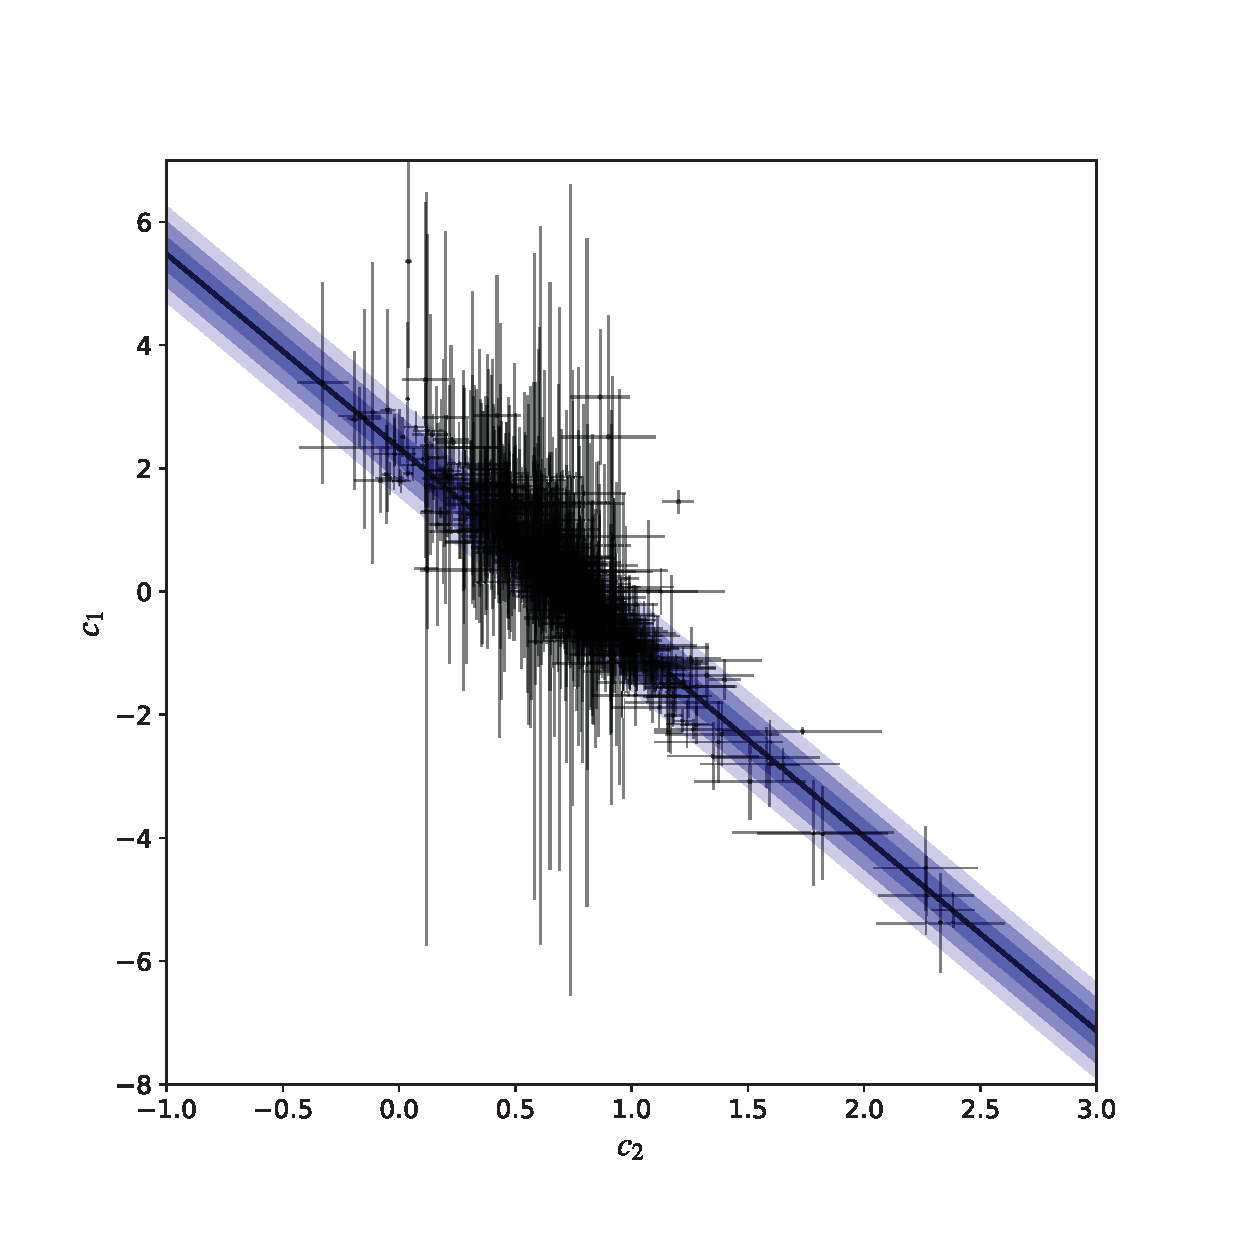
\includegraphics[width=1.0\linewidth]{figures/c1c2_data.eps}
    \caption{Observed $c_1$ vs $c_2$ data from \textcite{valencic04}, \textcite{gordon03}, \textcite{newdatafitzpatrick2007analysis}, and \textcite{m31dataclayton2015new}, plotted with linear TRK fit modeled by Equation \eqref{eq:c1c2model}. Shaded regions indicate the $1-$, $2-$ and $3\sigma$ slop confidence regions of the model distribution, given best fit slop values of Table \ref{table:c1c2} and plotted according to footnote \ref{footnote:modelcurvebands} on page \pageref{footnote:modelcurvebands}.}
    \label{fig:c1c2_data}
\end{figure}

\begin{figure}
    \centering
    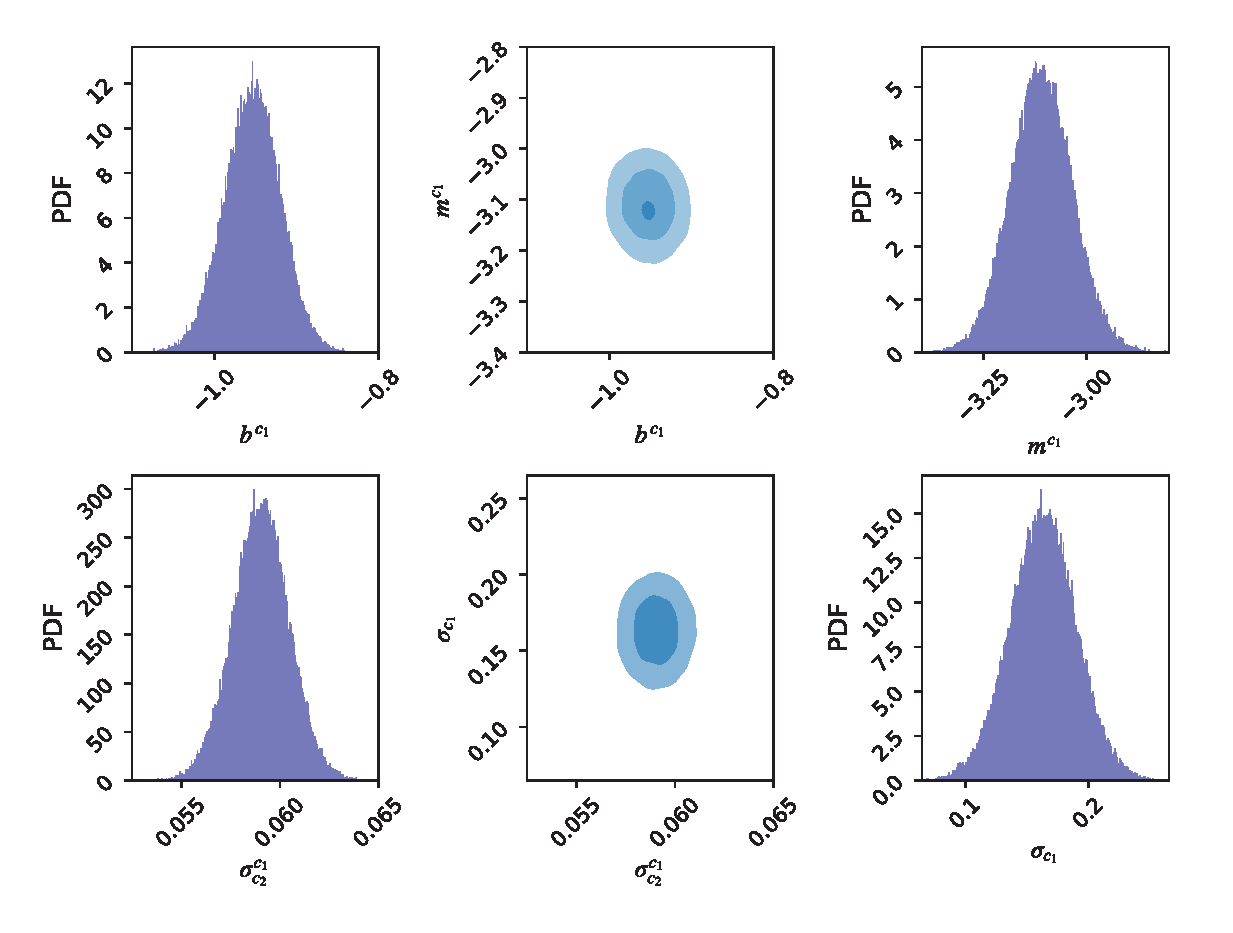
\includegraphics[width=1.0\linewidth]{figures/c1c2_params.eps}
    \caption{MCMC-generated (\S\ref{sec:MCMC}) probability distributions for $c_1$ vs. $c_2$ (Equation \eqref{eq:c1c2model}) model (top) and slop/extrinsic scatter (bottom) parameters. Parameter confidence ellipses (center) with $1-$, $2-$ and $3\sigma$ regions show joint posterior probabilities with respect to the parameters plotted on either side. The pivot-point finding algorithm of  \S\ref{sec:pivot} was used to remove correlation between model parameters.}
    \label{fig:c1c2_params}
\end{figure}

\begin{table}
\label{table:c1c2}
\caption{Best-Fit Asymmetric Gaussian Parameter Values For $c_1$ vs. $c_2$ Model (Equation \eqref{eq:c1c2model})}
\centering
\vspace{0.3cm}
\begin{tabular}{@{}lcccc@{}}
\toprule
Parameter Type   & Parameter            & Value    & \begin{tabular}[c]{@{}c@{}}$+1\sigma$\\ Width\end{tabular} & \begin{tabular}[c]{@{}c@{}}$-1\sigma$\\ Width\end{tabular} \\ \midrule
Model Parameters & $b^{c_1}$            & $-0.9052$  & 0.0350                                                     & $-0.0376$                                                    \\
                 & $m^{c_1}$            & $-3.1519$  & 0.0778                                                     & $-0.0762$                                                    \\
Pivot Point      & $c_2^{p_{c_2}}$      & 1.0247 & $\ldots$                                                   & $\ldots$                                                   \\
Slop Parameters  & $\sigma_{c_2}^{c_1}$ & 0.05948  & 0.00135                                                    & $-0.00148$                                                   \\
                 & $\sigma_{c_1}$       & 0.1711   & 0.0270                                                     & $-0.0263$                                                    \\
Optimum Scale    & $s_0$                & 0.28230  & $\ldots$                                                   & $\ldots$                                                   \\
Minimum Scale    & $a$                  & 0.15332  & $\ldots$                                                   & $\ldots$                                                   \\
Maximum Scale    & $b$                  & 0.44043  & $\ldots$                                                   & $\ldots$                                                   \\ \bottomrule
\end{tabular}
\end{table}

\subsection{Fitting $\text{BH}$ vs. $c_2$}

\textcite{trotter} also reported that the bump height parameter $\text{BH}\equiv c_3/\gamma^2$ is loosely correlated with $c_2$, as moderate values of $c_2$ tend to have higher values of $\text{BH}$ while low or high values of $c_2$ tend to have low $\text{BH}$, along Milky Way lines-of-sight. Trotter parameterized this relationship with a ``smoothly-broken linear'' model of the form
\begin{equation}\label{eq:bhc2model}
    \text{BH}_{c}(c_2;\vartheta_m)=-\ln\left[\exp{{-b_1^{\text{BH}}-\tan\theta_1^{\text{BH}}\left(c_2-c_2^{p_1,\text{BH}}\right)}}+\exp{{-b_2^{\text{BH}}-\tan\theta_2^{\text{BH}}\left(c_2-c_2^{p_2,\text{BH}}\right)}}\right],
\end{equation}
where $\vartheta_m=\{b_1^{\text{BH}}, \theta_1^{\text{BH}}, b_2^{\text{BH}}, \theta_2^{\text{BH}}\}$ are the model parameters and $\{c_2^{p_1,\text{BH}}, c_2^{p_2,\text{BH}}\}$ are the pivot points of the model that determine the amount of correlation between $b_1^{\text{BH}}$ and $\theta_1^{\text{BH}}$, and $b_2^{\text{BH}}$ and $\theta_2^{\text{BH}}$, respectively\footnote{To see the intuition behind this broken-linear parameterization, observe how for low $c_2$, the model approximately becomes linear, i.e. $\text{BH}_{c}(c_2;\vartheta_m)\simeq b_1^{\text{BH}}+\tan\theta_1^{\text{BH}}\left(c_2-c_2^{p_1,\text{BH}}\right)$. Similarly, for high $c_2$, $\text{BH}_{c}(c_2;\vartheta_m)\simeq b_2^{\text{BH}}+\tan\theta_2^{\text{BH}}\left(c_2-c_2^{p_2,\text{BH}}\right)$. As such, $b_1^{\text{BH}}$ and $b_2^{\text{BH}}$ are analogous to the intercept parameters for two lines, while $\theta_1^{\text{BH}}$ and $\theta_2^{\text{BH}}$ are analogous to (the angles off of the $c_2-$axis of) the slope parameters.}. 

To fit this model to the dataset, I first ran the scale optimization algorithm of \S\ref{sec:scaleop} to determine the optimum fitting scale $s_0$. Next, I ran the parameter correlation removal/pivot point-finding algorithm of \S\ref{sec:pivot} to determine the pivot points $c_2^{p_1,\text{BH}}$ and $c_2^{p_2,\text{BH}}$ that minimize the correlations between $b_1^{\text{BH}}$ and $\theta_1^{\text{BH}}$, and $b_2^{\text{BH}}$ and $\theta_2^{\text{BH}}$, respectively\footnote{Note that the pivot point-finding algorithm of \S\ref{sec:pivot} and Algorithm \ref{algo:pivotpoint} was only explicitly defined for models with a single pivot point. As such, I modified the code to allow for models that have multiple pivot points using a fairly straightforward generalization of Algorithm \ref{algo:pivotpoint}. Specifically, I used the MCMC-sampled pairs of slope and intercept parameters (line 6 of Algorithm \ref{algo:pivotpoint}) to compute and weight samples from successive distributions of possible pivot points (lines 8 through 17), in order to iteratively determine optimal values for the two pivot points (lines 19 and 20).}. From here, I determined the best fit model and $(x-,y-)$slop parameters $\vartheta_m=\{b_1^{\text{BH}}, \theta_1^{\text{BH}}, b_2^{\text{BH}}, \theta_2^{\text{BH}}\}$ and $(\sigma_{c_2}^{\text{BH}}, \sigma_{\text{BH}})$, respectively using the Downhill Simplex method of \S\ref{sec:simplex} at $s_0$. Finally, I used the Adaptive MCMC and Bar-Lowering methods of \S\ref{sec:MCMC} to sample the distribution of the model and slop parameters, and compute their uncertainties, respectively. Furthermore, for this fit I used priors on the slope angle parameters $\theta_1^{\text{BH}}$ and $\theta_2^{\text{BH}}$ to constrain the angles of the line to specific quadrants (also in order to demonstrate the usage of priors with the TRK suite) in the form of
\begin{equation}\label{eq:bhc2priors}
p(\theta_1^{\text{BH}}) =  \left\{ \begin{array} {lr}
        \mathcal{U}(\pi, \frac{3\pi}{2}) & \,\,\mbox{if $\theta_1^{\text{BH}} \in [\pi, \frac{3\pi}{2}]$}\, ,\\
        0 & \,\,\mbox{otherwise} \,
        \end{array}\right.
        \qquad
p(\theta_2^{\text{BH}}) =  \left\{ \begin{array} {lr}
        \mathcal{U}(-\frac{\pi}{2}, 0) & \,\,\mbox{if $\theta_2^{\text{BH}} \in [-\frac{\pi}{2}, 0]$}\, ,\\
        0 & \,\,\mbox{otherwise} \,,
        \end{array}\right.
\end{equation}
% {-0.5*PI, 0} };
where $\mathcal{U}(a,b)$ indicates a uniform distribution with bounds $a$ and $b$.

The numerical results of this fit are given in Table \ref{table:bhc2}, while the fit is plotted in Figure \ref{fig:bhc2_data} with generated model and slop parameter distributions shown in Figure \ref{fig:bhc2_params}. Note that because the pivot point-finding routine was used to minimize the correlation between $b_1^{\text{BH}}$ and $\theta_1^{\text{BH}}$, and $b_2^{\text{BH}}$ and $\theta_2^{\text{BH}}$, the confidence ellipses for these two pairs of parameters (top, center, and middle, center of Figure \ref{fig:bhc2_params}) are not tilted, indicating the removal of correlation between these sets of parameters. Finally, also note in this figure that the two slop parameters $(\sigma_{c_2}^{\text{BH}}$ and $\sigma_{\text{BH}})$ are also uncorrelated, again evidenced by a non-tilted confidence ellipse (bottom, center).

\begin{figure}
    \centering
    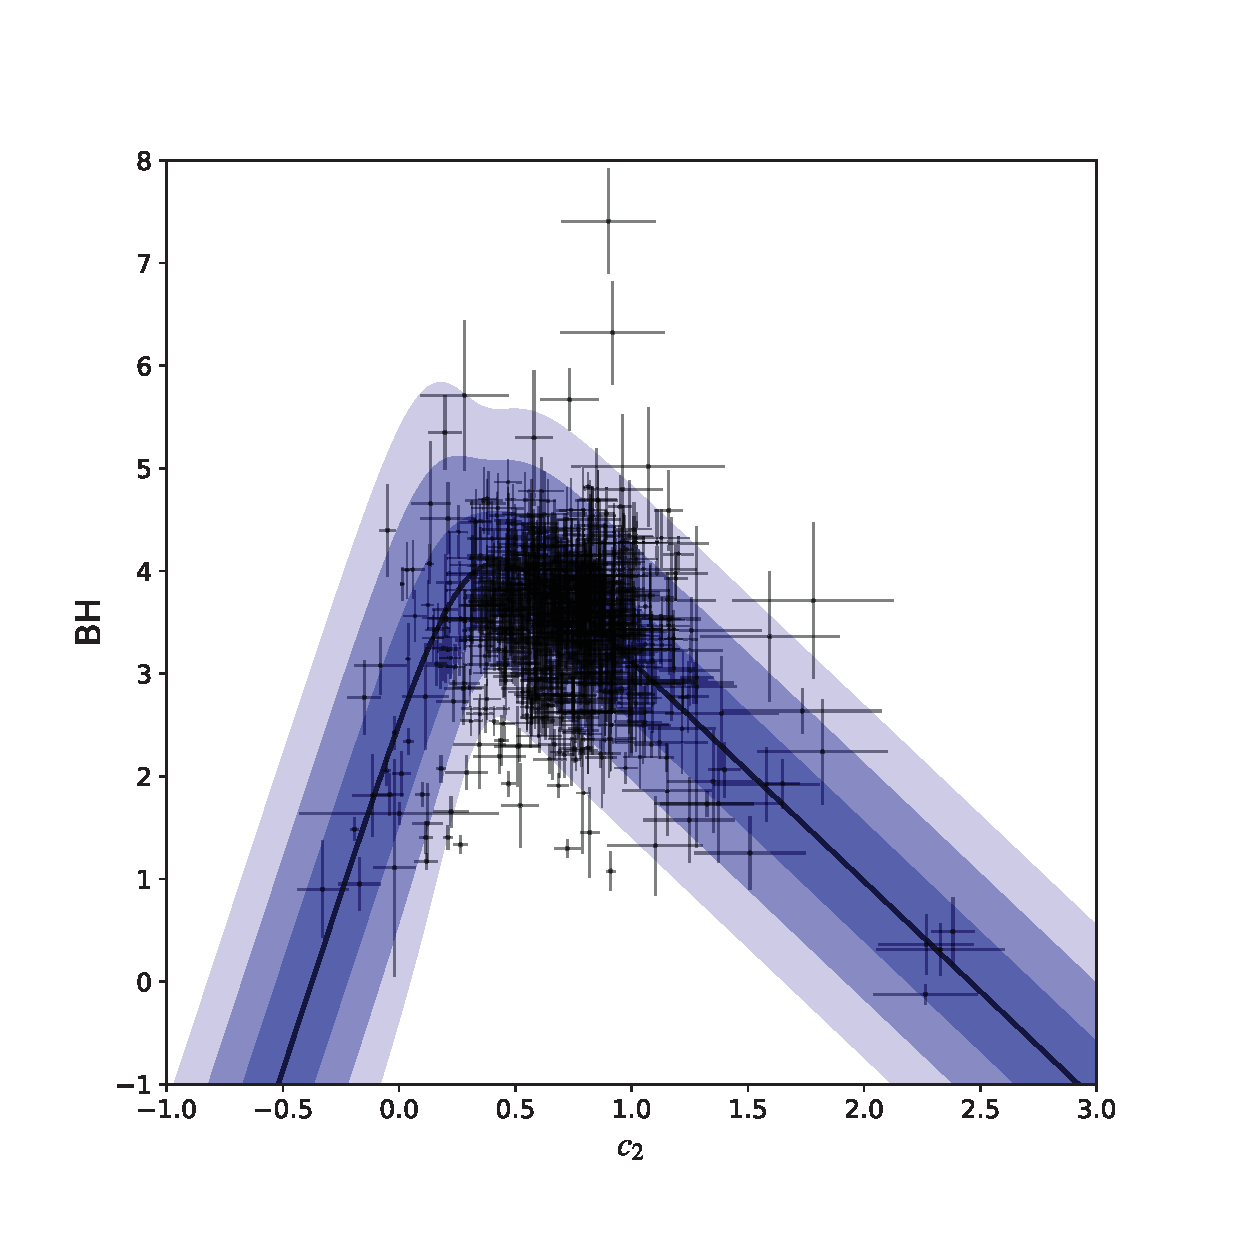
\includegraphics[width=1.0\linewidth]{figures/bhc2_data.eps}
    \caption{Observed $\text{BH}$ vs $c_2$ data from \textcite{valencic04}, \textcite{gordon03}, \textcite{newdatafitzpatrick2007analysis}, and \textcite{m31dataclayton2015new}, plotted with broken-linear TRK fit modeled by Equation \eqref{eq:bhc2model}. Shaded regions indicate the $1-$, $2-$ and $3\sigma$ slop confidence regions of the model distribution, given best fit slop values of Table \ref{table:bhc2} and plotted according to footnote \ref{footnote:modelcurvebands} on page \pageref{footnote:modelcurvebands}.}
    \label{fig:bhc2_data}
\end{figure}

\begin{figure}
    \centering
    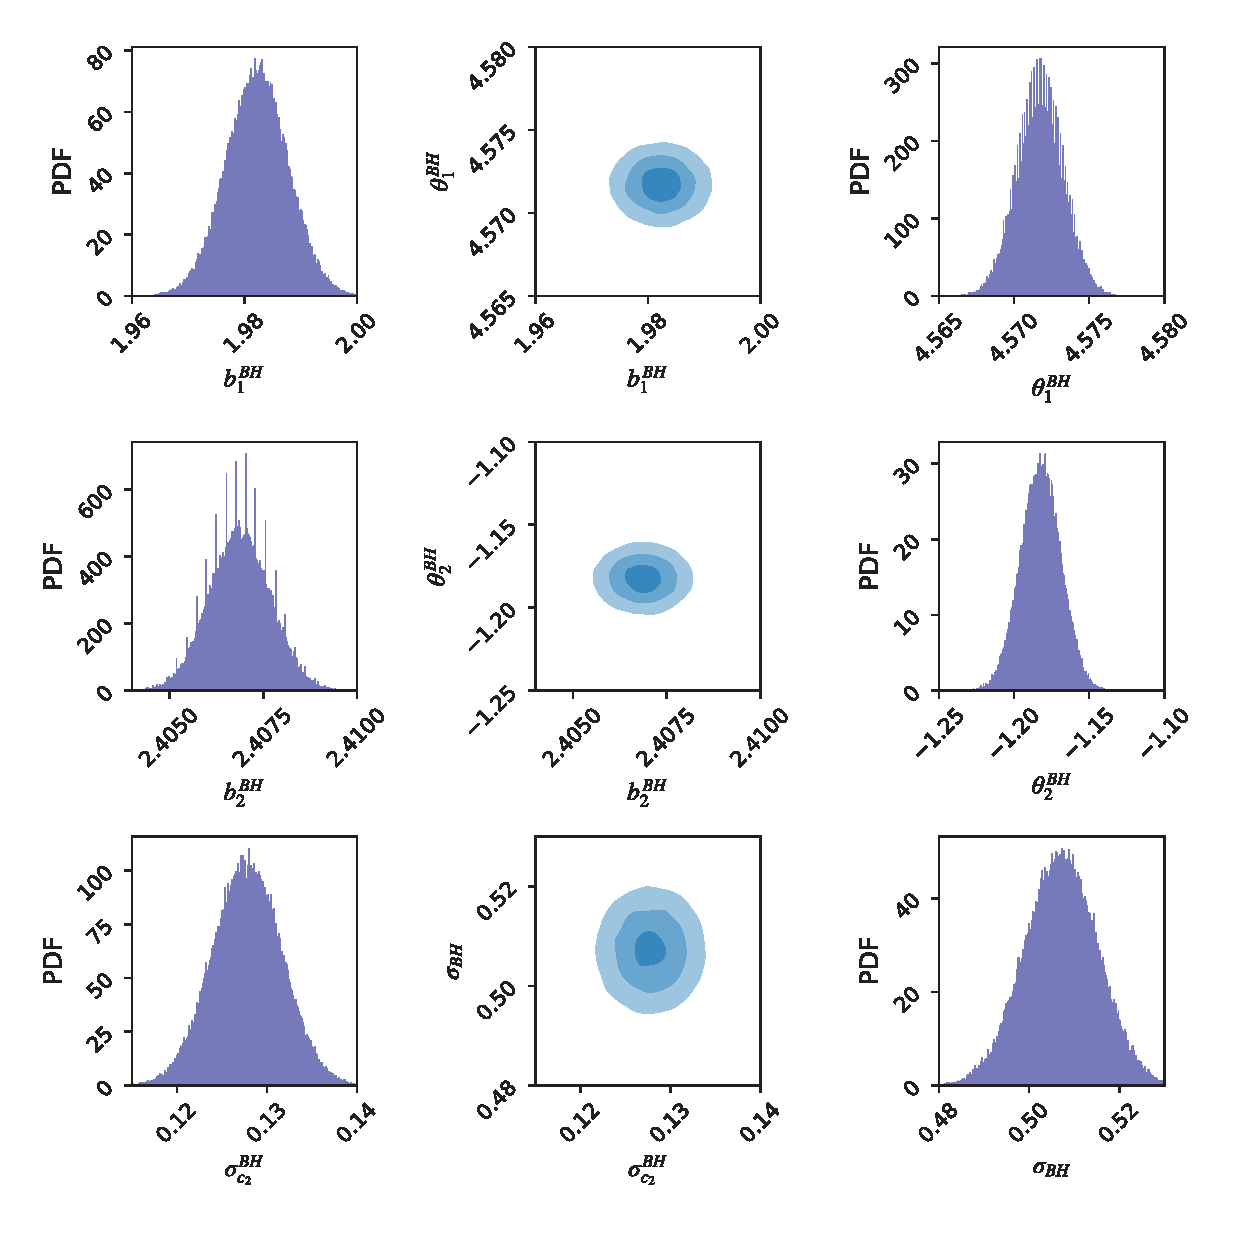
\includegraphics[width=1.0\linewidth]{figures/bhc2_params.eps}
    \caption{MCMC-generated (\S\ref{sec:MCMC}) probability distributions for $\text{BH}$ vs. $c_2$ (Equation \eqref{eq:bhc2model}) model (top and middle rows) and slop/extrinsic scatter (bottom row) parameters. Parameter confidence ellipses (center) with $1-$, $2-$ and $3\sigma$ regions show joint posterior probabilities with respect to the parameters plotted on either side. The pivot-point finding algorithm of \S\ref{sec:pivot} was used to remove respective correlations between model parameters of each linear "leg" of the model curve.}
    \label{fig:bhc2_params}
\end{figure}

\begin{table}
\label{table:bhc2}
\caption{Best-Fit Asymmetric Gaussian Parameter Values For $\text{BH}$ vs. $c_2$ Model (Equation \eqref{eq:bhc2model})}
\centering
\vspace{0.3cm}
\begin{tabular}{@{}lcccc@{}}
\toprule
Parameter Type   & Parameter            & Value    & \begin{tabular}[c]{@{}c@{}}$+1\sigma$\\ Width\end{tabular} & \begin{tabular}[c]{@{}c@{}}$-1\sigma$\\ Width\end{tabular} \\ \midrule
Model Parameters & $b_1^{\text{BH}}$            & 1.9837  &  0.0054                                                   &       $-0.0057$                      \\
                 & $\theta_1^{\text{BH}}$            & 4.5679  &  0.0016                                                    &    $-0.0015$                           \\
                 & $b_2^{\text{BH}}$            & 2.4040  &     0.0008                                                 &    $-0.0008$                                \\
                 & $\theta_2^{\text{BH}}$            & $-1.1344$  &  0.0130                                                    &   $-0.0138$                              \\
Pivot Points     & $c_2^{p_1,\text{BH}}$      & $-0.0867$ & $\ldots$                                                   & $\ldots$                                                   \\
                 & $c_2^{p_2,\text{BH}}$      & 1.3343 & $\ldots$                                                   & $\ldots$                                                   \\
Slop Parameters  & $\sigma_{c_2}^{\text{BH}}$ & 0.1290  &  0.0037                                                   &  $-0.0039$                                                  \\
                 & $\sigma_{\text{BH}}$       & 0.4954  &  0.0077                                                   & $-0.0081$                                                    \\
Optimum Scale    & $s_0$                & 0.28117  & $\ldots$                                                   & $\ldots$                                                   \\
Minimum Scale    & $a$                  & 0.11816  & $\ldots$                                                   & $\ldots$                                                   \\
Maximum Scale    & $b$                  & 0.94043  & $\ldots$                                                   & $\ldots$                                                   \\ \bottomrule
\end{tabular}
\end{table}

% \subsection{Fitting $R_V$ vs. $c_2$}
% \textcite{trotter} reported that the parameters $R_V$ and $c_2$ are loosely correlated, with low values of $c_2$ corresponding to very high values of $R_V$, and moderate or higher values of $c_2$ corresponding to the well known, approximately fixed value of $R_V\sim 3.1$. Trotter parameterized this relationship with a ``smoothly-broken linear'' model curve of the form 
% \begin{equation}\label{eq:rvc2model}
%     R_{V,c}(c_2;\vartheta_m)=\ln\left[\exp{{b_1^{R_V}+\tan\theta_1^{R_V}\left(c_2-c_2^{p_1,R_V}\right)}}+\exp{{b_2^{R_V}+\tan\theta_2^{R_V}\left(c_2-c_2^{p_2,R_V}\right)}}\right],
% \end{equation}
% where $\vartheta_m=\{b_1^{R_V}, \theta_1^{R_V}, b_2^{R_V}, \theta_2^{R_V}\}$ are the model parameters and $\{c_2^{p_1,R_V}, c_2^{p_2,R_V}\}$ are the pivot points of the model that determine the amount of correlation between $b_1^{R_V}$ and $\theta_1^{R_V}$, and $b_2^{R_V}$ and $\theta_2^{R_V}$, respectively.

% To fit this model to the dataset, I first ran the scale optimization algorithm of \S\ref{sec:scaleop} to determine the optimum fitting scale $s_0$. Next, I ran the parameter correlation removal/pivot point-finding algorithm of \S\ref{sec:pivot} to determine the pivot points $c_2^{p_1,R_V}$ and $c_2^{p_2,R_V}$ that minimizes the correlation between $b_1^{R_V}$ and $\theta_1^{R_V}$, and $b_2^{R_V}$ and $\theta_2^{R_V}$, respectively\footnote{Note that the pivot point-finding algorithm of \S\ref{sec:pivot} and Algorithm \ref{algo:pivotpoint} was only explicitly defined for models with a single pivot point. As such, I modified the code to allow for models that have multiple pivot points using a fairly straightforward generalization of Algorithm \ref{algo:pivotpoint}. Specifically, I used the MCMC-sampled pairs of slope and intercept parameters (line 6 of Algorithm \ref{algo:pivotpoint}) to compute and weight samples from successive distributions of possible pivot points (lines 8 through 17), in order to iteratively determine optimal values for the two pivot points (lines 19 and 20).}. From here, I determined the best fit model and $(x-,y-)$slop parameters $\vartheta_m=\{b^{c_1}, m^{c_1}\}$ and $(\sigma_{c_2}^{c_1}, \sigma_{c_1})$, respectively using the Downhill Simplex method of \S\ref{sec:simplex} at $s_0$\footnote{Note that I was able to run the scale optimization before finding the pivot point because fitting scales are invariant of choice of pivot point, as they don't affect the extreme scale limiting behavior of slops, e.g. \textcite{trotter}.}. Finally, I used the Adaptive MCMC and Bar-Lowering methods of \S\ref{sec:MCMC} to sample the distribution of the model and slop parameters, and compute their uncertainties, respectively. 

% The numerical results of this fit are given in Table \ref{table:c1c2}, while the fit is plotted in Figure \ref{fig:c1c2_data} with generated model and slop parameter distributions shown in Figure \ref{fig:c1c2_params}. In Figure \ref{fig:c1c2_data}, note the small slop confidence regions of the model distributiona about the model line, indicated a strong correlation between $c_1$ and $c_2$, as expected. Also, note that because the pivot point-finding routine was used to minimize the correlation between $b^{c_1}$ and $m^{c_1}$, the confidence ellipse for these two parameters (top, center of Figure \ref{fig:c1c2_params}) is not tilted, indicating the removal of correlation between them. Finally, also note in this figure that the two slop parameters $(\sigma_{c_2}^{c_1}$ and $\sigma_{c_1})$ are also uncorrelated, again evidenced by a non-tilted confidence ellipse (bottom, center).

% \begin{figure}
%     \centering
%     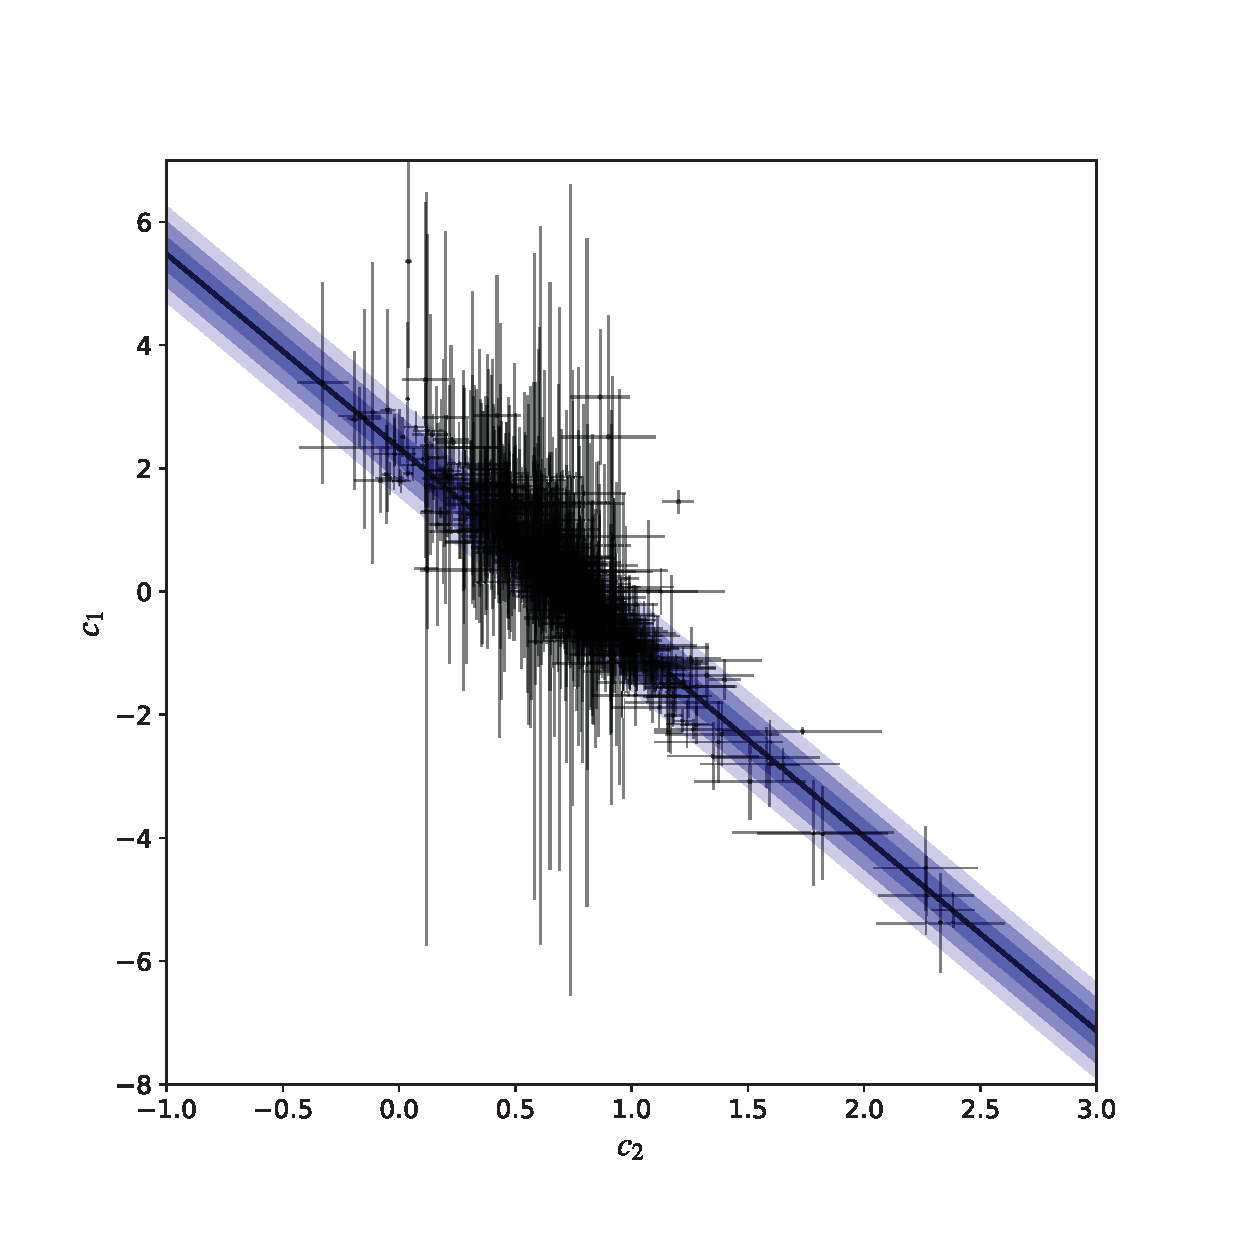
\includegraphics[width=1.0\linewidth]{figures/c1c2_data.eps}
%     \caption{Observed $R_V$ vs $c_2$ data from \textcite{valencic04}, \textcite{gordon03}, \textcite{newdatafitzpatrick2007analysis}, and \textcite{m31dataclayton2015new}, plotted with broken-linear TRK fit modeled by Equation \eqref{eq:rvc2model}. Shaded regions indicate the $1-$, $2-$ and $3\sigma$ slop confidence regions of the model distribution, given best fit slop values of Table \ref{table:rvc2} and plotted according to \ref{footnote:modelcurvebands} on page \pageref{footnote:modelcurvebands}.}
%     \label{fig:rvc2_data}
% \end{figure}

% \begin{figure}
%     \centering
%     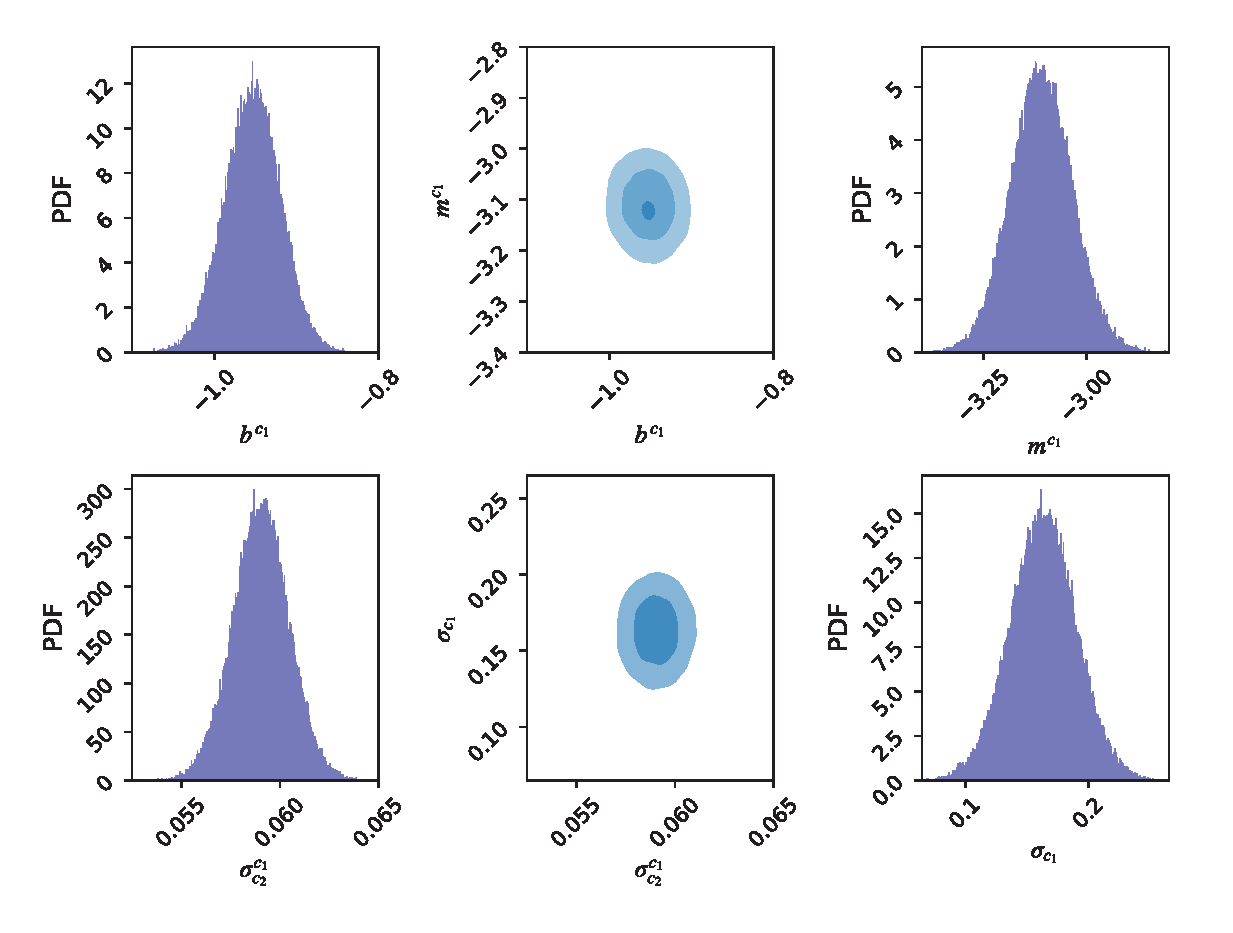
\includegraphics[width=1.0\linewidth]{figures/c1c2_params.eps}
%     \caption{MCMC-generated (\S\ref{sec:MCMC}) probability distributions for $R_V$ vs. $c_2$ (Equation \eqref{eq:rvc2model}) model (top and middle rows) and slop/extrinsic scatter (bottom row) parameters. Parameter confidence ellipses (center) with $1-$, $2-$ and $3\sigma$ regions show joint posterior probabilities with respect to the parameters plotted on either side. The pivot-point finding algorithm of \S\ref{sec:pivot} was used to remove respective correlations between model parameters of each linear "leg" of the model curve.}
%     \label{fig:rvc2_params}
% \end{figure}

% \begin{table}
% \label{table:c1c2}
% \caption{Best-Fit Asymmetric Gaussian Parameter Values For $R_V$ vs. $c_2$ Model (Equation \eqref{eq:rvc2model})}
% \centering
% \vspace{0.3cm}
% \begin{tabular}{@{}lcccc@{}}
% \toprule
% Parameter Type   & Parameter            & Value    & \begin{tabular}[c]{@{}c@{}}$+1\sigma$\\ Width\end{tabular} & \begin{tabular}[c]{@{}c@{}}$-1\sigma$\\ Width\end{tabular} \\ \midrule
% Model Parameters & $b_1^{R_V}$            &   &                                                     &                             \\
%                  & $\theta_1^{R_V}$            &   &                                                      &                               \\
%                  & $b_2^{R_V}$            &   &                                                      &                                    \\
%                  & $\theta_2^{R_V}$            &   &                                                      &                                 \\
% Pivot Points     & $c_2^{p_1,R_V}$      &  & $\ldots$                                                   & $\ldots$                                                   \\
%                  & $c_2^{p_2,R_V}$      &  & $\ldots$                                                   & $\ldots$                                                   \\
% Slop Parameters  & $\sigma_{c_2}^{R_V}$ &   &                                                     &                                                    \\
%                  & $\sigma_{R_V}$       &    &                                                      &                                                     \\
% Optimum Scale    & $s_0$                &   & $\ldots$                                                   & $\ldots$                                                   \\
% Minimum Scale    & $a$                  &   & $\ldots$                                                   & $\ldots$                                                   \\
% Maximum Scale    & $b$                  &   & $\ldots$                                                   & $\ldots$                                                   \\ \bottomrule
% \end{tabular}
% \end{table}

\section{A Web-Based TRK Fit Calculator}
\label{sec:website}
Alongside with the development of the TRK suite source code, the other main project that I undertook is the end-to-end development of a web-based calculator for running TRK fits, currently located at \url{https://skynet.unc.edu/rcr/calculator/trk}\footnote{Note that this is part of the website that also includes the two Robust Chauvenet Outlier Rejection (RCR) calculators (see \textcite{maples2018robust}), that I am also the developer of (both the RCR source code and webpages). Long term, I plan to develop a single standalone statistical suite, available in multiple languages, that will bring together RCR, TRK, and other future statistical tools that I've developed, of which this website will be part of the ecosystem of.}. Easy to use, but full of customization options, the goal of this website was to create a simple, user-friendly introduction to the TRK statistic, including educational interactive visualization tools.

The first step of the web-based TRK calculator is to input the raw data, shown in Figure \ref{fig:websiteinput}, where the user can give values for $\{x_n,\sigma_{x,n},y_n,\sigma_{y,n}\}$ with optional weights $\{w_n\}$.
\begin{figure}
    \centering
    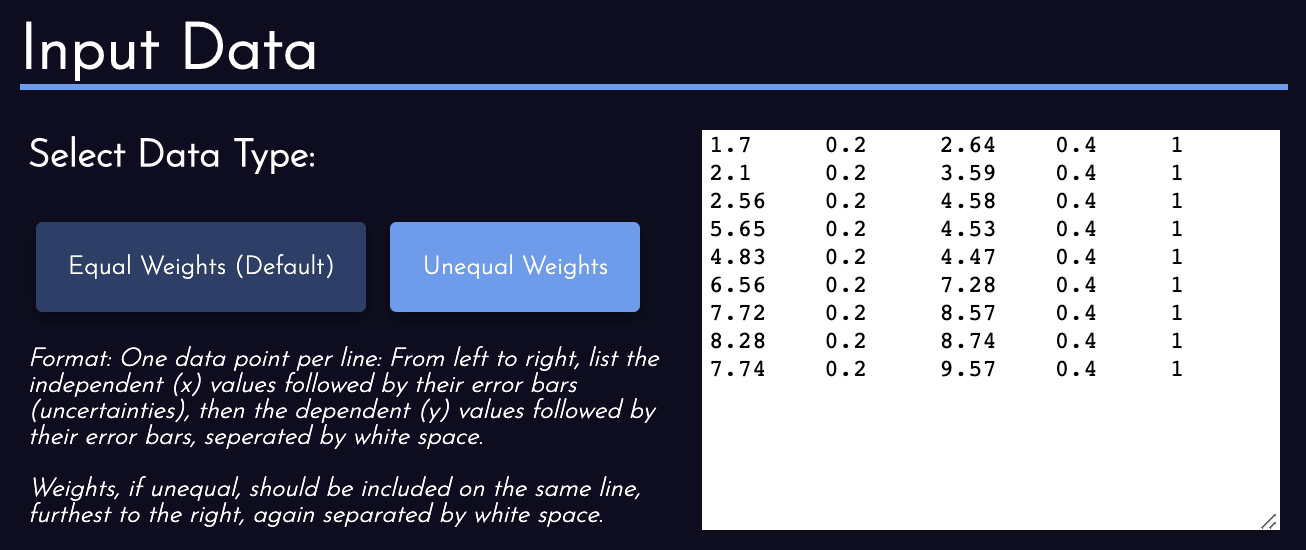
\includegraphics[width=1.0\linewidth]{figures/websiteinput.png}
    \caption{The data input step of the web-based TRK calculator with example data.}
    \label{fig:websiteinput}
\end{figure}
Next, shown in Figure \ref{fig:websiteinputplot}, the user can plot the data with error bars in order to estimate which model to fit to the data. The plot also offers various interactive tools, including the ability to pan and zoom\footnote{This plot, as well as all other plots on the TRK and RCR webpages, were made with Python's Bokeh library, from the \textcite{bokeh}.}.
\begin{figure}
    \centering
    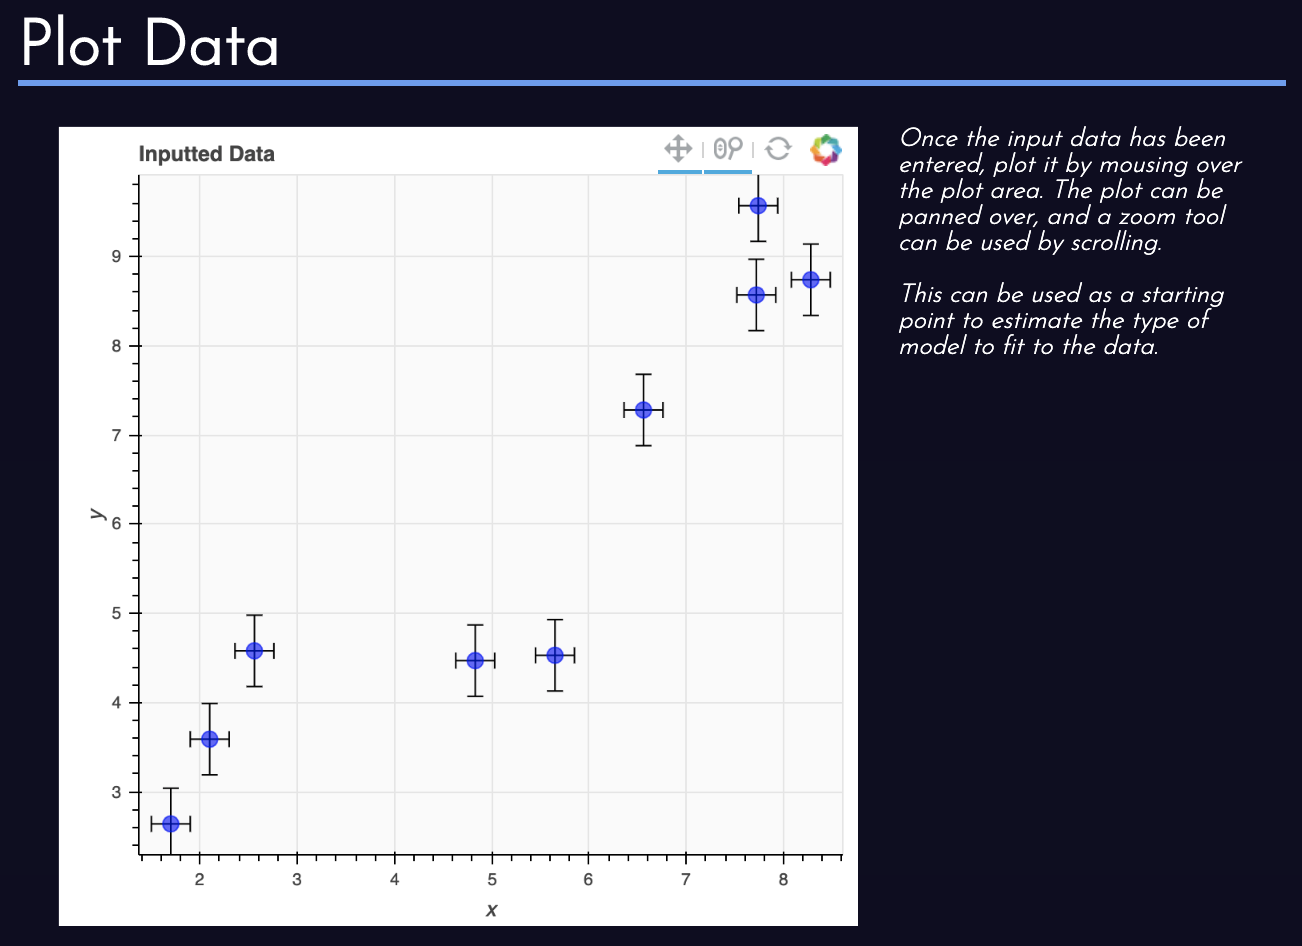
\includegraphics[width=1.0\linewidth]{figures/websiteinputplot.png}
    \caption{Example of plotting input data on the TRK calculator webpage.}
    \label{fig:websiteinputplot}
\end{figure}

The following step is then for the user to choose the model to fit the data to, shown in Figure \ref{fig:websitechoosemodel}, and to provide an initial guess for the model and slop parameters for the fitting algorithm. The website comes with six built-in models: linear, quadratic, cubic, exponential, power law and logarithmic; the user also has the option to run the pivot-point finding/de-correlation algorithm of \S\ref{sec:pivot} on applicable models.
\begin{figure}
    \centering
    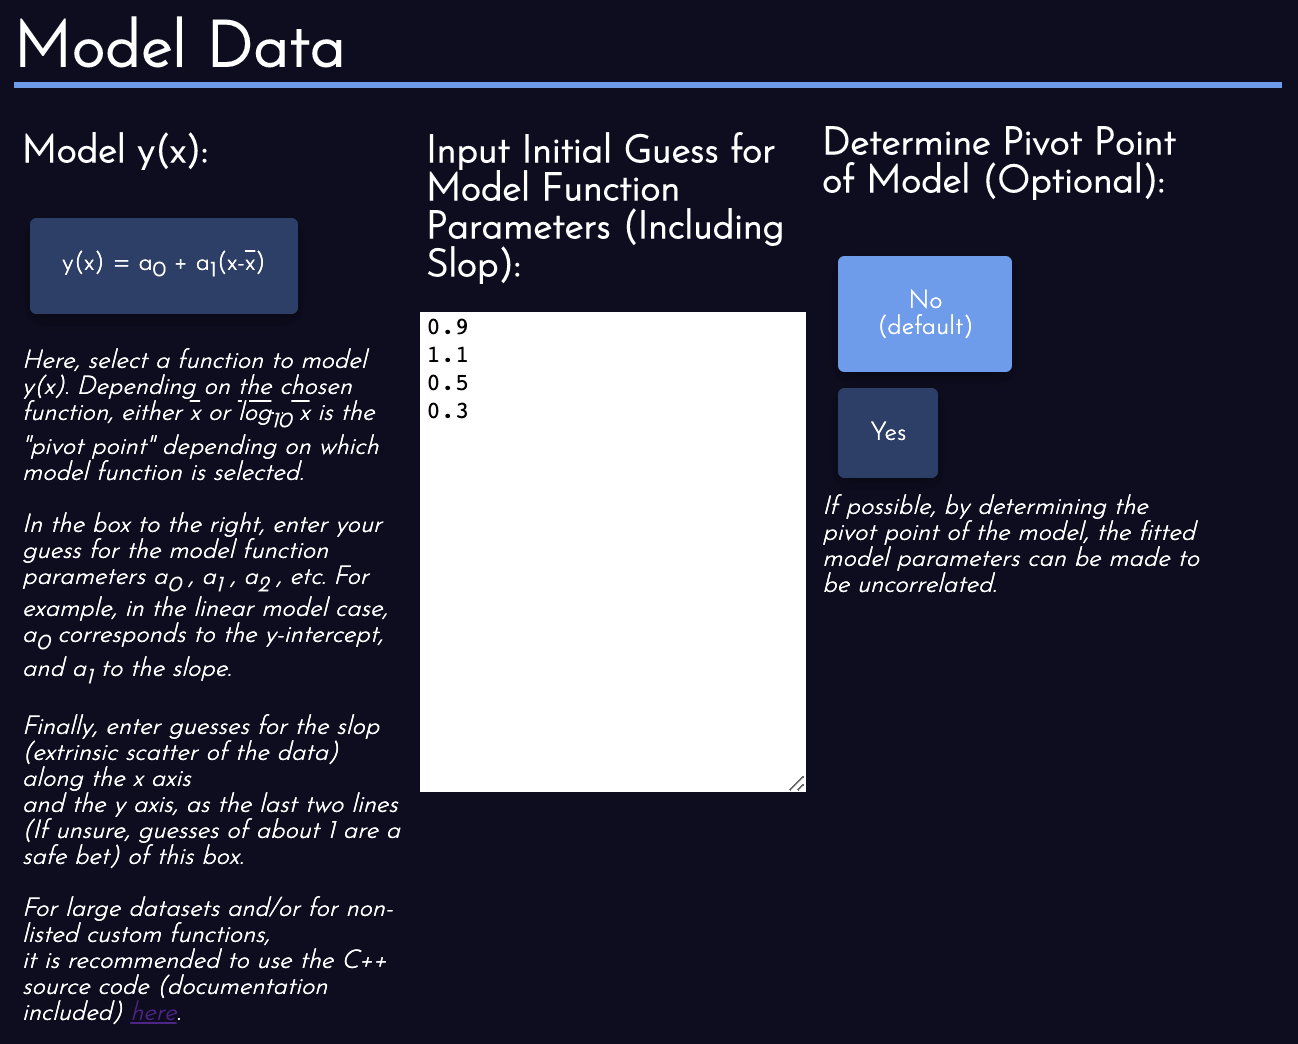
\includegraphics[width=1.0\linewidth]{figures/websitechoosemodel.png}
    \caption{Section of the TRK webpage where the user can choose which model to fit to their data.}
    \label{fig:websitechoosemodel}
\end{figure}

The last step of the calculator is for the user to choose which algorithms, if any, to run in addition to the regular likelihood-maximization downhill-simplex fitting of \S\ref{sec:simplex}, shown in Fig. \ref{fig:websitechoosealgo}. The user can choose to either provide a fitting scale $s$ (with a default of $s=1.0$), or run the scale optimization algorithm. The user also has the option to use the MCMC algorithm of \S\ref{sec:MCMC} to determine model parameter uncertainties; however, this is a timely process, so I am still experimenting with the possibility of expediting it. As shown, the total selected algorithm is displayed as a flow chart, with bullet-points below explaining the various steps\footnote{As shown, these bullet points also show section numbers; these correspond to the relavent sections of our upcoming paper, \textcite{TRKIapjs}, that will introduce the TRK statistic and some of its astrophysical applications in a peer-reviewed, journalistic context. The paper, currently in preparation, will be submitted to the Astrophysical Journal, Supplement Series.}.
\begin{figure}
    \centering
    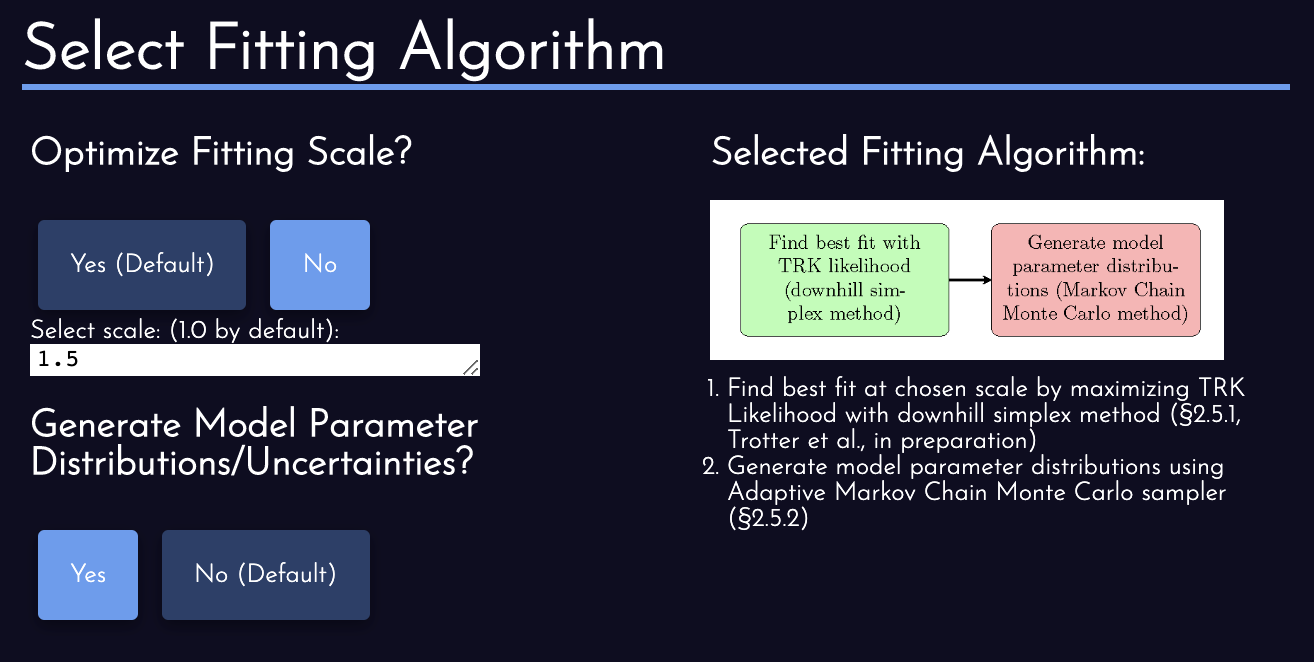
\includegraphics[width=1.0\linewidth]{figures/websitechoosealgo.png}
    \caption{Section of the TRK webpage where the user can determine which additional TRK algorithms to run alongside basic fit.}
    \label{fig:websitechoosealgo}
\end{figure}

With these steps completed, the user can now perform a TRK Fit, in the section shown in Figure \ref{fig:websiteoutput}. After pressing the ``Perform Fit'' button and waiting for the algorithm to run, the final model and slop parameters will be displayed on the left, as shown (with the model parameter ordered according to the functional form of the chosen model). If the scale optimization algorithm was run, the optimum and extreme scales, $(s_0,a,b)$, respectively, will also be displayed. The resulting fitted model curve will then be plotted alongside the data, including 1-, 2- and $3\sigma$ confidence regions described by the fitted slop parameters (see Footnote \ref{footnote:modelcurvebands} on page \pageref{footnote:modelcurvebands} to see how these regions are explicitly calculated).
\begin{figure}
    \centering
    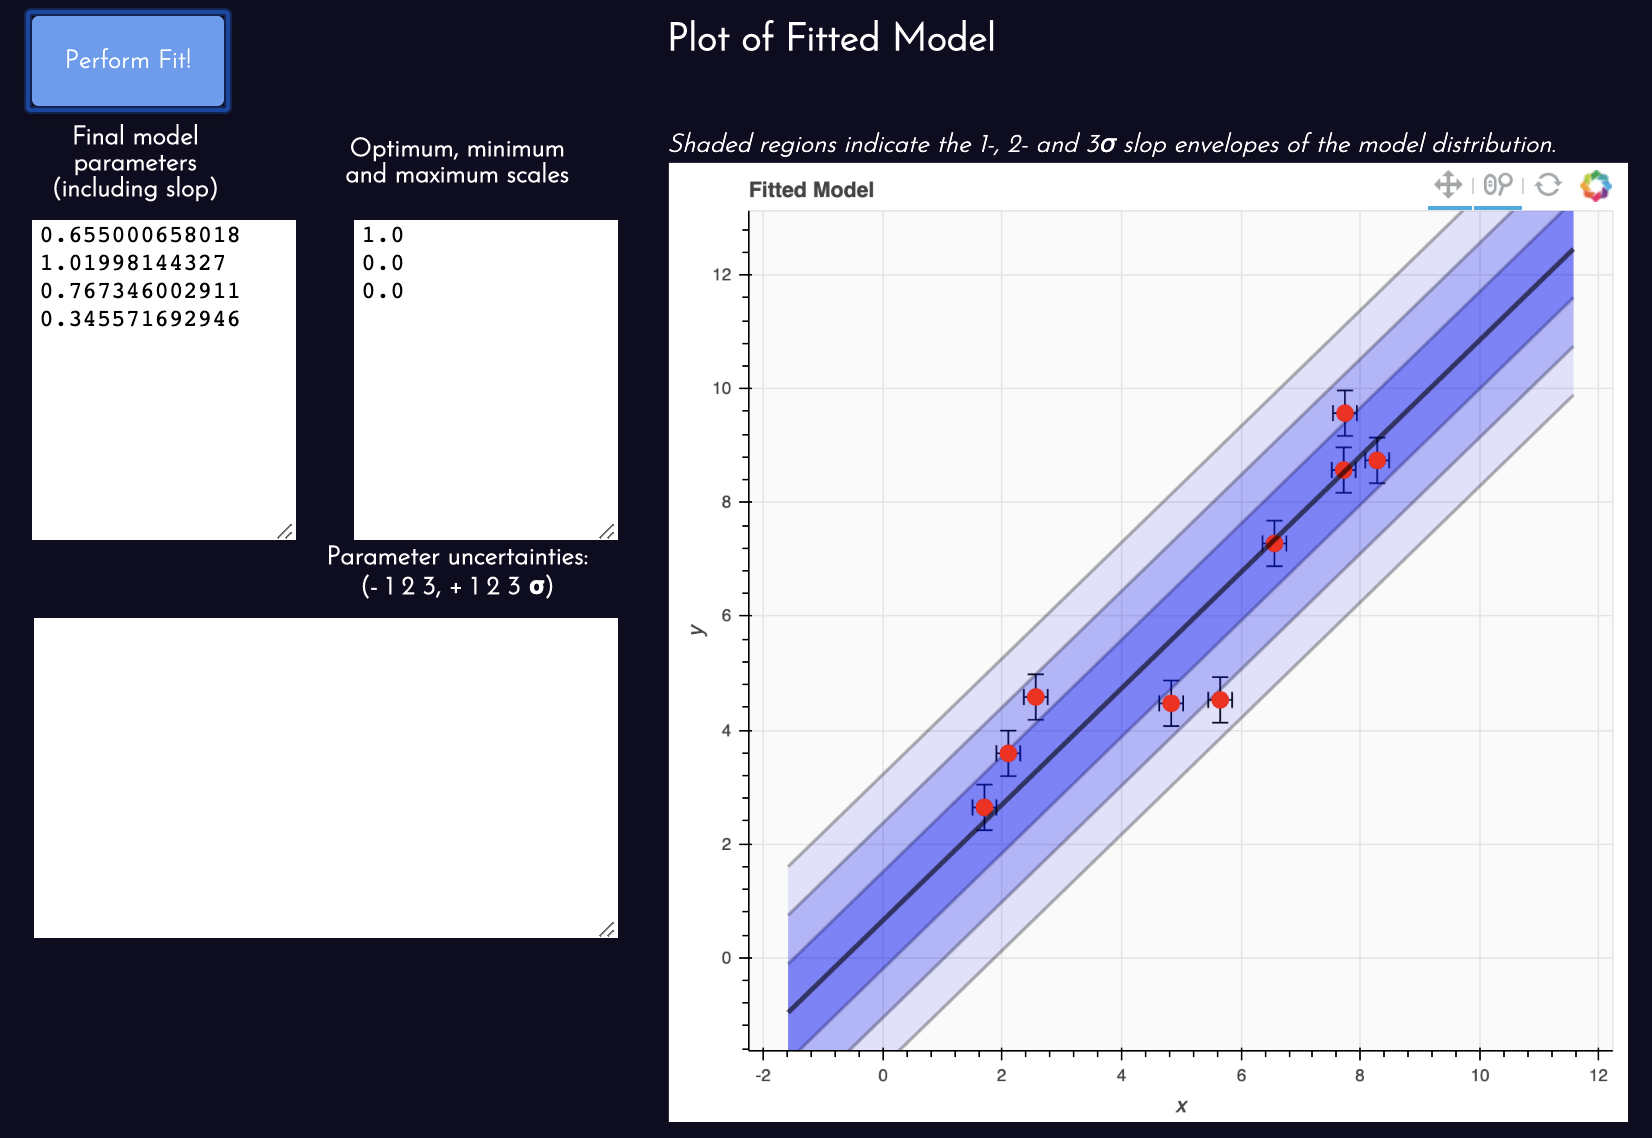
\includegraphics[width=1.0\linewidth]{figures/websiteoutput.png}
    \caption{Output section of the TRK calculator webpage, showing the results of an example linear fit (without model parameter uncertainty computation).}
    \label{fig:websiteoutput}
\end{figure}             %% this is a suggestion: you have to create this file on demand

\chapter{Future Endeavors}
\label{cha:future}

\section{A Scale Optimization Algorithm for Asymmetric Uncertainties}
Continuing from \S\ref{sec:asymm}, the final consideration to be made involving the introduction of asymmetric error bars and/or slop is the \textit{fit scale optimization} algorithm described in \S\ref{sec:scaleop}. Recall that in the symmetric case, this involves
\begin{enumerate}
    \item determining the minimum scale $s=a$ where $\sigma_x\rightarrow 0$, and the maximum scale $s=b$ where $\sigma_y\rightarrow 0$, and
    \item determining the optimum fitting scale $s_0\in [a,b]$ by iteratively solving Equation \eqref{eq:r2TRK}.
\end{enumerate}
However, in the asymmetric case there are \textit{two} slop parameters along each dimension, so determining, or even qualifying, the minimum, maximum and optimum scales is nontrivial. I have attempted and/or posited a few potential methods of asymmetric scale optimization, and tested the scale-dependent best fit behavior of asymmetric fits, but the results have been inconclusive as of late. As such, this issue remains as a future endeavor that will be explored in a later work.

\section{Support for $N$-dimensional Models}
For any statistic, it is desirable to be able to fit models to data with \textit{multiple} independent (``$x$'') variables. I have considered the possibility of generalizing the TRK statistic to $N-1$ independent variables (so $N$ dimensions total) such that each datapoint could have $N$ symmetric error bars, or up to $2N$ asymmetric error bars, and the model would have $N$ parameters describing slop/extrinsic scatter. However, there are a number of practical issues that could make this leap of faith difficult, or potentially intractable. First, the tangent-point finding algorithm of \S\ref{sec:tgtpts} and \S\ref{sec:tgtfinder}, that is required to simply evaluate the TRK likelihood of Equation \eqref{eq:TRK}, would require determining where some $N-$dimensional model curve is tangent to an $N-$dimensional error hyperellipsoid, which would not only conceivably greatly increase the computational power and possible issues with the method, but would require a totally new algorithm to account for the arbitrary number of dimensions. Even more fundamentally, the scale optimization routine of \S\ref{sec:scaleop} would also have to be completely revamped, as not only is it entirely based off of 2-dimensional principles and algorithms, but the definition itself of fitting scale would have to change with addition of more dimensions, as adding $N$ dimensions means there are now $N$ possible ways to scale the dataset, described by $N$ additional scale parameters. Overall, while an $N-$dimensional TRK statistic and algorithm would be extremely useful, and practically the ultimate general ``worst-case'' dataset model-fitting tool, developing it would likely prove to be very challenging, if even possible.

\section{Python Implementation}
I developed the TRK suite in C++ due to the language's portability, low-level nature, and access to parallelization, to name a few reasons. However, Python is one of the most popular and widespread languages used within data science, the natural sciences, and other related statistically-based fields. Some of the most used model fitting algorithms are found within the many scientific Python libraries, such as SciPy (e.g. \textcite{2020SciPy-NMeth}), and introducing the TRK suite to Python could make it accessible and useful to many more people, and make it possible to integrate and use the TRK statistic with many other Python codebases. As such, another long-term goal of this project is to develop/port the TRK suite into a standalone Python library. This could be done in many ways, but the main option I am currently considering is using SWIG (Simple Wrapper Interface Generator of \textcite{beazley1996swig}) to wrap the C++ TRK code into Python, which I did at a basic level when developing the TRK calculator, as the website runs on a Python-based framework.
  

\appendix                       %% closes main document, appendix follows until end; only available in book-classes
%\addpart*{Appendix}             %% adding Appendix to tableofcontents
\chapter{Additional Algorithm Listings}
\label{app:algos}
%\section{From \S\ref{sec:tgtfinder}}
%\section{From \S\ref{sec:simplex}}
Listed below are various algorithms that did not need to be given explicitly in the main text, but can be referenced here as needed.
\begin{algorithm}
\label{algo:simplexsteps}
\caption{Downhill simplex evolution functions used in Algorithm \ref{algo:simplex} to minimize $-2\ln\mathcal{L}^\text{TRK}$.}
\DontPrintSemicolon
    \SetKwInOut{Input}{Input}
    \SetKwInOut{Output}{Output}
    \SetKwProg{Fn}{Function}{}{}
    Initialize simplex evolution parameters $(\alpha,\beta,\gamma,\delta)=(1,2,0.5,0.5)$\;
    \Fn{Expand}{
        \Input{Simplex $\Delta$ with $\mathcal{M}+1$ vertices $v_i$}
        \Output{Expanded $\Delta$}
        Compute expansion point of $v_r$, $v_e\equiv c + \gamma(v_r-c)$.\;
        \If{$\chi^2_e < \chi^2_r$}{
            $v_\mathcal{M}\rightarrow v_e$\;
        }
        \Else{
            $v_\mathcal{M}\rightarrow v_r$\;
        }
        \Return{$\Delta$}
    }
    \Fn{Contract}{
        \Input{Simplex $\Delta$ with $\mathcal{M}+1$ vertices $v_i$}
        \Output{Contracted $\Delta$}
        Compute contraction point $v_c$, by using better of $v_\mathcal{M}$, $v_r$.\;
        \If{$\chi^2_{\mathcal{M}-1} \leq \chi^2_r < \chi^2_{\mathcal{M}}$}{
            \textit{Contract Outside:}\;
            $v_c = c+\beta(v_r-c)$\;
            \If{$\chi^2_c\leq\chi^2_r$}{
                $v_\mathcal{M}\rightarrow v_c$
            }
            \Else{
                \textit{Shrink}$(\Delta)$ (\textit{See function below})\;
            }
        }
        \ElseIf{$\chi^2_r\geq chi^2_\mathcal{M}$}{
            \textit{Contract Inside:}\;
            $v_c = c+\beta(v_\mathcal{M}-c)$\;
            \If{$\chi^2_c<\chi^2_\mathcal{M}$}{
                $v_\mathcal{M}\rightarrow v_c$
            }
            \Else{
                \textit{Shrink}$(\Delta)$\;
            }
        }
        \Return{$\Delta$}
    }
    \Fn{Shrink}{
        \Input{Simplex $\Delta$ with $\mathcal{M}+1$ vertices $v_i$}
        \Output{Shrunken $\Delta$}
        \For{$i=0,\cdots,\mathcal{M}$}{
            $v_i \rightarrow v_0 + \delta(v_i-v_0)$\;
        }
        \Return{$\Delta$}
    }
\end{algorithm}

\begin{algorithm}
\label{algo:maxscale}
\caption{Bracketing/Bisection-type method for determining maximum fitting scale $b$ for some model and dataset.}
\DontPrintSemicolon
    \SetKwInOut{Input}{Input}
    \SetKwInOut{Output}{Output}
    \SetKwProg{Fn}{Function}{}{}
    \Fn{FindMinimumScale}{
        \Input{Model $y_c$ and dataset $\{x_n,y_n\}$ with error bars $\{\sigma_{x,n}, \sigma_{y,n}\}$}
        \Output{Maximum fitting scale $b$.}
        \Begin{
            \textit{Determine brackets $(l,r)$ for max scale $b$:}\;
            Initialize bisection brackets $l = s = 0, r = s = 1$ and $s_\text{trial} = s = 1$\;
            \textit{Note that in the actual code, a better $s_\text{trial}$ is found from the algorithm for finding $a$.}
            $\sigma_y(s_\text{trial}) \leftarrow $\textit{ DownhillSimplex}($s=s_\text{trial}$)\;
            Initialize step modifier $\alpha = 0.5\times s_\text{trial}$\;
            \If{$\sigma_y(s_\text{trial}) > 0$}{
                $l = s_\text{trial}$\;
                $r_\text{trial}=s_\text{trial}$\;
                $\sigma_y(r_\text{trial})=$\textit{DownhillSimplex}($s=r_\text{trial}$)\;
                \While{$\sigma_y(r_\text{trial}) > 0$}{
                    $r_\text{trial} = r_\text{trial}+\alpha$\;
                    $\sigma_y(r_\text{trial})=$\textit{DownhillSimplex}($s=r_\text{trial}$)\;
                    $l=r_\text{trial}$\;
                }
                $r=r_\text{trial}$\;
            }
            \ElseIf{$\sigma_y(s_\text{trial}) = 0$}{
                $r = s_\text{trial}$\;
                $l_\text{trial}=s_\text{trial}$\;
                $\sigma_y(l_\text{trial})=$\textit{DownhillSimplex}($s=l_\text{trial}$)\;
                \While{$\sigma_x(l_\text{trial}) = 0$}{
                    $l_\text{trial} = l_\text{trial}-\alpha$\;
                    $\sigma_y(l_\text{trial})=$\textit{DownhillSimplex}($s=l_\text{trial}$)\;
                    $\alpha = 0.5\times\alpha$\;
                    $r=l_\text{trial}$\;
                }
                $l=l_\text{trial}$\;
            }
            \textit{Use bisection to determine $b$ now that we have brackets $(l,r)$:}\;
            $b_\text{trial} = (l+r)/2$\;
            $\sigma_y(b_\text{trial})=$\textit{DownhillSimplex}($s=b_\text{trial}$)\;
            \While{$\abs{l-r}\geq$ tolerance1 AND $\sigma_y(a_\text{trial})\geq$ tolerance2}{
                $b_\text{trial} = (l+r)/2$\;
                $\sigma_y(b_\text{trial})=$\textit{DownhillSimplex}($s=b_\text{trial}$)\;
                \If{$\sigma_y(b_\text{trial})>0$}{
                    $l = b_\text{trial}$\;
                }
                \ElseIf{$\sigma_y(b_\text{trial})=0$}{
                    $r = b_\text{trial}$\;
                }
            }
            \Return{$b=b_\text{trial}$}
        }
    }
\end{algorithm}

\begin{algorithm}
\label{algo:opscaler2}
\caption{Bisection-type method for determining optimum fitting scale $s_0$ for some model and dataset with minimum and maximum fitting scales $a$ and $b$.}
\DontPrintSemicolon
    \SetKwInOut{Input}{Input}
    \SetKwInOut{Output}{Output}
    \SetKwProg{Fn}{Function}{}{}
    \Fn{FindOptimumScale}{
        \Input{Model $y_c$ and dataset $\{x_n,y_n\}$ with error bars $\{\sigma_{x,n}, \sigma_{y,n}\}$, with minimum and maximum fitting scale $a$ and $b$.}
        \Output{Optimum fitting scale $s_0$.}
        \Begin{
            Initialize $s_0^{(1)}=(a+b)/2$\;
            \While{$\abs{s_0^{(2)} - s_0^{(1)}} \geq$ tolerance1}{
                $s_0^{(1)} = s_0^{(2)}$\;
                \textit{Use bisection to determine $s_0^{(2)}$ given $s_0^{(1)}$:}\;
                Initialize brackets $l=a$, $r=b$\;
                $s_{0,\text{trial}}^{(2)} = (l+r)/2$\;
                $R_\text{trial}=$ Equation \eqref{eq:r2TRKnewscalenum} $\leftarrow$\textit{DownhillSimplex}($s=s_{0,\text{trial}}^{(2)}$)\;
                \While{$\abs{l-r}\geq$ tolerance2 AND $\abs{R} \geq 0$}{
                    $s_{0,\text{trial}}^{(2)} = (l+r)/2$\;
                    $R_\text{trial}=$ Equation \eqref{eq:r2TRKnewscalenum} $\leftarrow$\textit{DownhillSimplex}($s=s_{0,\text{trial}}^{(2)}$)\;
                    $R_l=$ Equation \eqref{eq:r2TRKnewscalenum} $\leftarrow$\textit{DownhillSimplex}($s=l$)\;
                    \If{$R_\text{trial}\times R_l>0$}{
                        $l = s_{0,\text{trial}}^{(2)}$\;
                    }
                    \ElseIf{$R_\text{trial}\times R_l<0$}{
                        $r = s_{0,\text{trial}}^{(2)}$\;
                    }
                }
                $s_0^{(2)} = s_{0,\text{trial}}^{(2)}$\;
            }
            \Return{Optimum scale $s_0=s_0^{(2)}$}\;
        }
    }
\end{algorithm}

\printbibliography              %% remove, if using BibTeX instead of biblatex
% \include{further_ressources}  %% this is a suggestion: you have to create this file on demand





%%%% end{document}
\end{document}
%% vim:foldmethod=expr
%% vim:fde=getline(v\:lnum)=~'^%%%%\ .\\+'?'>1'\:'='
%%% Local Variables:
%%% mode: latex
%%% mode: auto-fill
%%% mode: flyspell
%%% eval: (ispell-change-dictionary "en_US")
%%% TeX-master: "main"
%%% End:
